\documentclass[a4paper,11pt,english]{report}

%%%% pour compiler avec variables d'environnement et retirer les problemes d'_:
%% pdflatex -interaction=nonstopmode -jobname=Generic_Guide '\begingroup\lccode`~=`_ \lowercase{\endgroup\let~}_ \catcode`_=12\def \TRUSTROOTLATEX {$(TRUST_ROOT)} \def \TRUSTV {$(TRUST_VERSION)} \def \BALTROOT {$(project_directory)} \documentclass[a4paper,11pt,english]{report}

%%%% pour compiler avec variables d'environnement et retirer les problemes d'_:
%% pdflatex -interaction=nonstopmode -jobname=Generic_Guide '\begingroup\lccode`~=`_ \lowercase{\endgroup\let~}_ \catcode`_=12\def \TRUSTROOTLATEX {$(TRUST_ROOT)} \def \TRUSTV {$(TRUST_VERSION)} \def \BALTROOT {$(project_directory)} \documentclass[a4paper,11pt,english]{report}

%%%% pour compiler avec variables d'environnement et retirer les problemes d'_:
%% pdflatex -interaction=nonstopmode -jobname=Generic_Guide '\begingroup\lccode`~=`_ \lowercase{\endgroup\let~}_ \catcode`_=12\def \TRUSTROOTLATEX {$(TRUST_ROOT)} \def \TRUSTV {$(TRUST_VERSION)} \def \BALTROOT {$(project_directory)} \documentclass[a4paper,11pt,english]{report}

%%%% pour compiler avec variables d'environnement et retirer les problemes d'_:
%% pdflatex -interaction=nonstopmode -jobname=Generic_Guide '\begingroup\lccode`~=`_ \lowercase{\endgroup\let~}_ \catcode`_=12\def \TRUSTROOTLATEX {$(TRUST_ROOT)} \def \TRUSTV {$(TRUST_VERSION)} \def \BALTROOT {$(project_directory)} \input{Generic_Guide}'

\usepackage[unicode=true,pdfusetitle, bookmarks=true,bookmarksnumbered=false,bookmarksopen=false,
 breaklinks=false,pdfborder={0 0 1},backref=false,colorlinks=true,linkcolor=blue,pageanchor, urlcolor=darkblue]
 {hyperref}[2010/09/11]

\ifx \TRUSTV \undefined
\def\TRUSTVERSION{}
\else
\def\TRUSTVERSION{V\TRUSTV}
\fi
%\def \REFERENCEMANUAL {../../Outils/TRIOXDATA/XTriou/doc.pdf}
\def \REFERENCEMANUAL {TRUST_Reference_Manual.pdf}

\hypersetup{pdftitle={TRUST Generic Guide \TRUSTVERSION}, pdfauthor={Team TRUST} }

\usepackage[utf8]{inputenc}
\usepackage[T1]{fontenc}
\usepackage[top=2cm, bottom=2cm, left=2cm, right=2cm]{geometry}
\usepackage{babel}
\usepackage{alltt}
\usepackage{color}
\usepackage{longtable}
\usepackage{tikz}
\usepackage{xspace}
\usepackage{graphicx}
%\usepackage{times}

\setlength{\parindent}{0pt} % pas d'indentation

\definecolor{darkblue}{HTML}{3535B4}
\definecolor{LightSkyBlue}{HTML}{87CFFA}
\definecolor{DeepSkyBlue}{HTML}{00BFFF}
\definecolor{Greeen}{HTML}{439236}
\definecolor{mauve}{HTML}{874ad3}
\definecolor{vert}{HTML}{0ab351}
\definecolor{darkred}{HTML}{a31623}

\newenvironment{remark}{\textit{\underline{Remark:}}}{}
\newcommand{\trust}{\textbf{TRUST}\xspace}
\newcommand{\trustref}{Project\xspace}
\newcommand{\Note}{\textbf{\textcolor{darkred}{Note}}\xspace}


\begin{document}

\title{\vspace{2cm}\Huge \bfseries{TRUST Generic Guide \TRUSTVERSION}}
\author{
\vspace{2cm} % espace entre support team et ref manual
\LARGE \textbf{Support team: \href{mailto:triou@cea.fr}{triou@cea.fr}} \\
\vspace{1cm} % espace entre ref manual et la date
Link to: \LARGE \textbf{\href{run:\REFERENCEMANUAL}{\trustref Reference Manual}}\\
%%%%%%% Pour recuperer l'adresse d'un pdf par les variables d'environnement et makefile
%%%%%\ifx \BALTROOT \empty
%%%%%Link to: \LARGE \textbf{\href{run:\TRUSTROOTLATEX/Outils/TRIOXDATA/XTriou/doc.pdf}{\trustref Reference Manual}}\\
%%%%%\else
%%%%%Link to: \LARGE \textbf{\href{run:\BALTROOT/build/xdata/XTriou/doc.pdf}{\trustref Reference Manual}}\\
%%%%%\fi
}
%\date{} % si on ne veut pas la date

\maketitle
\tableofcontents{}
\newpage


%%%%%%%%%%%%%%%%%%%%%%%%%%%%%%%%%%%%%%%%%%%%%%%%%%%%%%%%%%%%%%%%%%%%%%%%
%
\chapter{Introduction}
%
%%%%%%%%%%%%%%%%%%%%%%%%%%%%%%%%%%%%%%%%%%%%%%%%%%%%%%%%%%%%%%%%%%%%%%%%
\input{chap1_intro.tex}
%%%%%%%%%%%%%%%%%%%%%%%%%%%%%%%%%%%%%%%%%%%%%%%%%%%%%%%%%%%%%%%%%%%%%%%%



%%%%%%%%%%%%%%%%%%%%%%%%%%%%%%%%%%%%%%%%%%%%%%%%%%%%%%%%%%%%%%%%%%%%%%%%
%
\chapter{Important references}
%
%%%%%%%%%%%%%%%%%%%%%%%%%%%%%%%%%%%%%%%%%%%%%%%%%%%%%%%%%%%%%%%%%%%%%%%%
\input{chap2_refs.tex}
%%%%%%%%%%%%%%%%%%%%%%%%%%%%%%%%%%%%%%%%%%%%%%%%%%%%%%%%%%%%%%%%%%%%%%%%



%%%%%%%%%%%%%%%%%%%%%%%%%%%%%%%%%%%%%%%%%%%%%%%%%%%%%%%%%%%%%%%%%%%%%%%%
%
\chapter{Data setting}
%
%%%%%%%%%%%%%%%%%%%%%%%%%%%%%%%%%%%%%%%%%%%%%%%%%%%%%%%%%%%%%%%%%%%%%%%%
\input{chap3_data_setting.tex}
%%%%%%%%%%%%%%%%%%%%%%%%%%%%%%%%%%%%%%%%%%%%%%%%%%%%%%%%%%%%%%%%%%%%%%%%



%%%%%%%%%%%%%%%%%%%%%%%%%%%%%%%%%%%%%%%%%%%%%%%%%%%%%%%%%%%%%%%%%%%%%%%%
%
\chapter{Problem definition}
%
%%%%%%%%%%%%%%%%%%%%%%%%%%%%%%%%%%%%%%%%%%%%%%%%%%%%%%%%%%%%%%%%%%%%%%%%
\input{chap4_problem_definition.tex}
%%%%%%%%%%%%%%%%%%%%%%%%%%%%%%%%%%%%%%%%%%%%%%%%%%%%%%%%%%%%%%%%%%%%%%%%



%%%%%%%%%%%%%%%%%%%%%%%%%%%%%%%%%%%%%%%%%%%%%%%%%%%%%%%%%%%%%%%%%%%%%%%%
%
\chapter{End of the data file}
%
%%%%%%%%%%%%%%%%%%%%%%%%%%%%%%%%%%%%%%%%%%%%%%%%%%%%%%%%%%%%%%%%%%%%%%%%
\input{chap5_ending.tex}
%%%%%%%%%%%%%%%%%%%%%%%%%%%%%%%%%%%%%%%%%%%%%%%%%%%%%%%%%%%%%%%%%%%%%%%%



%%%%%%%%%%%%%%%%%%%%%%%%%%%%%%%%%%%%%%%%%%%%%%%%%%%%%%%%%%%%%%%%%%%%%%%%
%
\chapter{Post-processing}
%
%%%%%%%%%%%%%%%%%%%%%%%%%%%%%%%%%%%%%%%%%%%%%%%%%%%%%%%%%%%%%%%%%%%%%%%%
\input{chap6_post_processing.tex}
%%%%%%%%%%%%%%%%%%%%%%%%%%%%%%%%%%%%%%%%%%%%%%%%%%%%%%%%%%%%%%%%%%%%%%%%



%%%%%%%%%%%%%%%%%%%%%%%%%%%%%%%%%%%%%%%%%%%%%%%%%%%%%%%%%%%%%%%%%%%%%%%%
%
\chapter{Parallel calculation} \label{parallel}
%
%%%%%%%%%%%%%%%%%%%%%%%%%%%%%%%%%%%%%%%%%%%%%%%%%%%%%%%%%%%%%%%%%%%%%%%%
\input{chap7_parallel.tex}
%%%%%%%%%%%%%%%%%%%%%%%%%%%%%%%%%%%%%%%%%%%%%%%%%%%%%%%%%%%%%%%%%%%%%%%%



%%%%%%%%%%%%%%%%%%%%%%%%%%%%%%%%%%%%%%%%%%%%%%%%%%%%%%%%%%%%%%%%%%%%%%%%%%
%%%
%%\chapter{Automatic validation form}
%%%
%%%%%%%%%%%%%%%%%%%%%%%%%%%%%%%%%%%%%%%%%%%%%%%%%%%%%%%%%%%%%%%%%%%%%%%%%%
%%%\input{chap8_prm.tex}
%%%%%%%%%%%%%%%%%%%%%%%%%%%%%%%%%%%%%%%%%%%%%%%%%%%%%%%%%%%%%%%%%%%%%%%%%%



\end{document}

'

\usepackage[unicode=true,pdfusetitle, bookmarks=true,bookmarksnumbered=false,bookmarksopen=false,
 breaklinks=false,pdfborder={0 0 1},backref=false,colorlinks=true,linkcolor=blue,pageanchor, urlcolor=darkblue]
 {hyperref}[2010/09/11]

\ifx \TRUSTV \undefined
\def\TRUSTVERSION{}
\else
\def\TRUSTVERSION{V\TRUSTV}
\fi
%\def \REFERENCEMANUAL {../../Outils/TRIOXDATA/XTriou/doc.pdf}
\def \REFERENCEMANUAL {TRUST_Reference_Manual.pdf}

\hypersetup{pdftitle={TRUST Generic Guide \TRUSTVERSION}, pdfauthor={Team TRUST} }

\usepackage[utf8]{inputenc}
\usepackage[T1]{fontenc}
\usepackage[top=2cm, bottom=2cm, left=2cm, right=2cm]{geometry}
\usepackage{babel}
\usepackage{alltt}
\usepackage{color}
\usepackage{longtable}
\usepackage{tikz}
\usepackage{xspace}
\usepackage{graphicx}
%\usepackage{times}

\setlength{\parindent}{0pt} % pas d'indentation

\definecolor{darkblue}{HTML}{3535B4}
\definecolor{LightSkyBlue}{HTML}{87CFFA}
\definecolor{DeepSkyBlue}{HTML}{00BFFF}
\definecolor{Greeen}{HTML}{439236}
\definecolor{mauve}{HTML}{874ad3}
\definecolor{vert}{HTML}{0ab351}
\definecolor{darkred}{HTML}{a31623}

\newenvironment{remark}{\textit{\underline{Remark:}}}{}
\newcommand{\trust}{\textbf{TRUST}\xspace}
\newcommand{\trustref}{Project\xspace}
\newcommand{\Note}{\textbf{\textcolor{darkred}{Note}}\xspace}


\begin{document}

\title{\vspace{2cm}\Huge \bfseries{TRUST Generic Guide \TRUSTVERSION}}
\author{
\vspace{2cm} % espace entre support team et ref manual
\LARGE \textbf{Support team: \href{mailto:triou@cea.fr}{triou@cea.fr}} \\
\vspace{1cm} % espace entre ref manual et la date
Link to: \LARGE \textbf{\href{run:\REFERENCEMANUAL}{\trustref Reference Manual}}\\
%%%%%%% Pour recuperer l'adresse d'un pdf par les variables d'environnement et makefile
%%%%%\ifx \BALTROOT \empty
%%%%%Link to: \LARGE \textbf{\href{run:\TRUSTROOTLATEX/Outils/TRIOXDATA/XTriou/doc.pdf}{\trustref Reference Manual}}\\
%%%%%\else
%%%%%Link to: \LARGE \textbf{\href{run:\BALTROOT/build/xdata/XTriou/doc.pdf}{\trustref Reference Manual}}\\
%%%%%\fi
}
%\date{} % si on ne veut pas la date

\maketitle
\tableofcontents{}
\newpage


%%%%%%%%%%%%%%%%%%%%%%%%%%%%%%%%%%%%%%%%%%%%%%%%%%%%%%%%%%%%%%%%%%%%%%%%
%
\chapter{Introduction}
%
%%%%%%%%%%%%%%%%%%%%%%%%%%%%%%%%%%%%%%%%%%%%%%%%%%%%%%%%%%%%%%%%%%%%%%%%
This document constitutes the generic guide for \textbf{TRUST software} and its \textbf{Baltik projects}.\\

\trust is a thermohydraulic software package for CFD simulations for incompressible monophasic flow.\\

You can create new project based on \trust plateform. Theses projects are named \textbf{"BALTIK"} projects.\\

The currently available modules include a VDF calculation module "Finite Difference Volume", a VEF calculation module "Finite Element Volume" and a PolyMAC module "series of Marker-and-Cell (MAC) schemes that can handle any type of mesh (non-conform, non-orthogonal, poly-hedral types, ...)". For further details, you can see https://cea-trust-platform.github.io/classes/discretizations/ \\

The VDF and VEF validated modules are designed to process the 2D or 3D flow of Newtonian, incompressible, weakly expandable fluids the density of which is a function of a local temperature and concentration values (Boussinesq approximation).



%%%%%%%%%%%%%%%%%%%%%%%%%%%%%%%%%%%%%%%%%%%%%%%%%%%%%%%%%%%%%%%
\section{Before TRUST: a modular software named Trio\_U}
%%%%%%%%%%%%%%%%%%%%%%%%%%%%%%%%%%%%%%%%%%%%%%%%%%%%%%%%%%%%%%%

\trust was born from the cutting in two pieces of \textbf{Trio\_U} software.
\textbf{Trio\_U} was a software brick based on the \textbf{Kernel} brick (which contains the equations, space discretizations, numerical schemes, parallelism...) and used by other CEA applications (cf Figure \ref{TrioU}).

\begin{figure}[h!]
\begin{center}
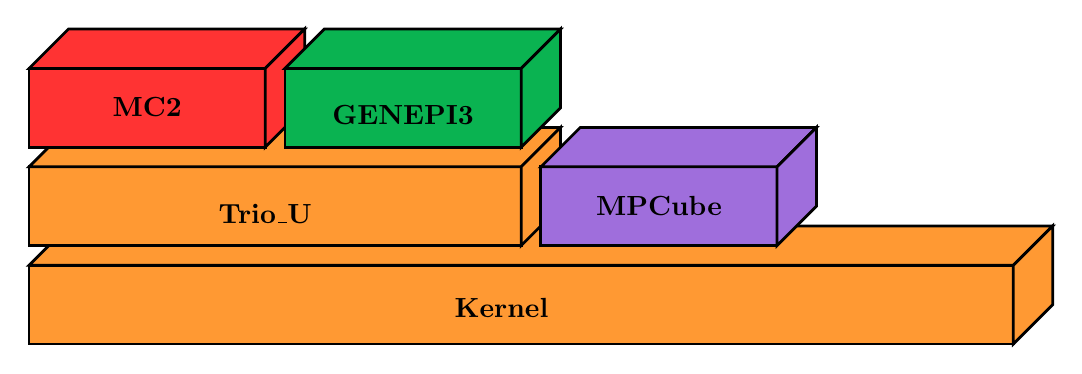
\begin{tikzpicture}[scale=2, line width=1pt]
% box Kernel
\coordinate (A) at (0,0) ;
\coordinate (B) at (6.25,0) ;
\coordinate (C) at (6.25,0.5) ;
\coordinate (D) at (0,0.5) ;
\coordinate (E) at (0.25,0.75) ;
\coordinate (F) at (6.5,0.75) ;
\coordinate (G) at (6.5,0.25) ;
\draw[black,fill=orange!80] (A) -- (B) -- (C) -- (D) -- cycle ;
\draw[black,fill=orange!80] (D) -- (C) -- (F) -- (E) -- cycle ;
\draw[black,fill=orange!80] (B) -- (C) -- (F) -- (G) -- cycle ;
\draw (3,0.1) node[above]{\textbf{Kernel}} ;
%% box Trio_U
\begin{scope}
\coordinate (A1) at (0,0.625) ;
\coordinate (B1) at (3.125,0.625) ;
\coordinate (C1) at (3.125,1.125) ;
\coordinate (D1) at (0,1.125) ;
\coordinate (E1) at (0.25,1.375) ;
\coordinate (F1) at (3.375,1.375) ;
\coordinate (G1) at (3.375,0.875) ;
\draw[black,fill=orange!80] (A1) -- (B1) -- (C1) -- (D1) -- cycle ;
\draw[black,fill=orange!80] (D1) -- (C1) -- (F1) -- (E1) -- cycle ;
\draw[black,fill=orange!80] (B1) -- (C1) -- (F1) -- (G1) -- cycle ;
\draw (1.5,0.7) node[above]{\textbf{Trio\_U}} ;
\end{scope}
% box MPCube
\begin{scope}[xshift=3.25 cm]
\coordinate (A1) at (0,0.625) ;
\coordinate (B1) at (1.5,0.625) ;
\coordinate (C1) at (1.5,1.125) ;
\coordinate (D1) at (0,1.125) ;
\coordinate (E1) at (0.25,1.375) ;
\coordinate (F1) at (1.75,1.375) ;
\coordinate (G1) at (1.75,0.875) ;
\draw[black,fill=mauve!80] (A1) -- (B1) -- (C1) -- (D1) -- cycle ;
\draw[black,fill=mauve!80] (D1) -- (C1) -- (F1) -- (E1) -- cycle ;
\draw[black,fill=mauve!80] (B1) -- (C1) -- (F1) -- (G1) -- cycle ;
\draw (0.75,0.75) node[above]{\textbf{MPCube}} ;
\end{scope}
%% box MC2
\begin{scope}[xshift=0 cm, yshift=0.625 cm]
\coordinate (A1) at (0,0.625) ;
\coordinate (B1) at (1.5,0.625) ;
\coordinate (C1) at (1.5,1.125) ;
\coordinate (D1) at (0,1.125) ;
\coordinate (E1) at (0.25,1.375) ;
\coordinate (F1) at (1.75,1.375) ;
\coordinate (G1) at (1.75,0.875) ;
\draw[black,fill=red!80] (A1) -- (B1) -- (C1) -- (D1) -- cycle ;
\draw[black,fill=red!80] (D1) -- (C1) -- (F1) -- (E1) -- cycle ;
\draw[black,fill=red!80] (B1) -- (C1) -- (F1) -- (G1) -- cycle ;
\draw (0.75,0.75) node[above]{\textbf{MC2}} ;
\end{scope}
% box GENEPI3
\begin{scope}[xshift=1.625 cm, yshift=0.625 cm]
\coordinate (A1) at (0,0.625) ;
\coordinate (B1) at (1.5,0.625) ;
\coordinate (C1) at (1.5,1.125) ;
\coordinate (D1) at (0,1.125) ;
\coordinate (E1) at (0.25,1.375) ;
\coordinate (F1) at (1.75,1.375) ;
\coordinate (G1) at (1.75,0.875) ;
\draw[black,fill=vert] (A1) -- (B1) -- (C1) -- (D1) -- cycle ;
\draw[black,fill=vert] (D1) -- (C1) -- (F1) -- (E1) -- cycle ;
\draw[black,fill=vert] (B1) -- (C1) -- (F1) -- (G1) -- cycle ;
\draw (0.75,0.7) node[above]{\textbf{GENEPI3}} ;
\end{scope}
\end{tikzpicture}
\caption{Trio\_U: brick software}
\label{TrioU}
\end{center}
\end{figure}

We could create new projects based on Kernel brick or \textbf{Trio\_U} brick. 
Theses projects were named \textbf{"BALTIK"} projects: "\textbf{B}uild an \textbf{A}pplication \textbf{L}inked to \textbf{T}r\textbf{I}o\_U \textbf{K}ernel".\\

In 2015, \textbf{Trio\_U} was divided in two parts: \trust and \textbf{TrioCFD}.
\begin{itemize}
\item \trust is a new platform, its name means: "\textbf{TR}io\_\textbf{U} \textbf{S}oftware for \textbf{T}hermohydraulics",
\item \textbf{TrioCFD} is a BALTIK project based on \trust, which contains the following models: FT, Radiation, LES, zoom...
\end{itemize}

Here is the structure of \trust platform (cf Figure \ref{TRUST}):

\begin{figure}[h!]
\begin{center}
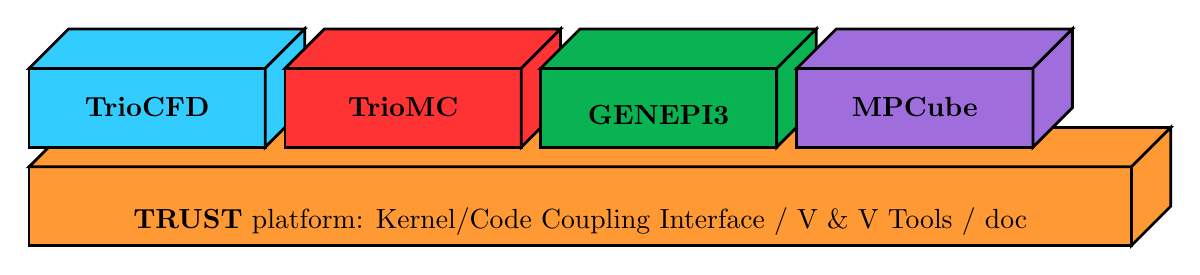
\begin{tikzpicture}[scale=2, line width=1pt]
% box TRUST
\coordinate (A) at (0,0) ;
\coordinate (B) at (7,0) ;
\coordinate (C) at (7,0.5) ;
\coordinate (D) at (0,0.5) ;
\coordinate (E) at (0.25,0.75) ;
\coordinate (F) at (7.25,0.75) ;
\coordinate (G) at (7.25,0.25) ;
\draw[black,fill=orange!80] (A) -- (B) -- (C) -- (D) -- cycle ;
\draw[black,fill=orange!80] (D) -- (C) -- (F) -- (E) -- cycle ;
\draw[black,fill=orange!80] (B) -- (C) -- (F) -- (G) -- cycle ;
\draw (3.5,0) node[above]{\trust platform: Kernel/Code Coupling Interface / V \& V Tools / doc} ;
%% box TrioCFD
\begin{scope}
\coordinate (A1) at (0,0.625) ;
\coordinate (B1) at (1.5,0.625) ;
\coordinate (C1) at (1.5,1.125) ;
\coordinate (D1) at (0,1.125) ;
\coordinate (E1) at (0.25,1.375) ;
\coordinate (F1) at (1.75,1.375) ;
\coordinate (G1) at (1.75,0.875) ;
\draw[black,fill=DeepSkyBlue!80] (A1) -- (B1) -- (C1) -- (D1) -- cycle ;
\draw[black,fill=DeepSkyBlue!80] (D1) -- (C1) -- (F1) -- (E1) -- cycle ;
\draw[black,fill=DeepSkyBlue!80] (B1) -- (C1) -- (F1) -- (G1) -- cycle ;
\draw (0.75,0.75) node[above]{\textbf{TrioCFD}} ;
\end{scope}
% box TrioMC
\begin{scope}[xshift=1.625 cm]
\coordinate (A1) at (0,0.625) ;
\coordinate (B1) at (1.5,0.625) ;
\coordinate (C1) at (1.5,1.125) ;
\coordinate (D1) at (0,1.125) ;
\coordinate (E1) at (0.25,1.375) ;
\coordinate (F1) at (1.75,1.375) ;
\coordinate (G1) at (1.75,0.875) ;
\draw[black,fill=red!80] (A1) -- (B1) -- (C1) -- (D1) -- cycle ;
\draw[black,fill=red!80] (D1) -- (C1) -- (F1) -- (E1) -- cycle ;
\draw[black,fill=red!80] (B1) -- (C1) -- (F1) -- (G1) -- cycle ;
\draw (0.75,0.75) node[above]{\textbf{TrioMC}} ;
\end{scope}
% box GENEPI3
\begin{scope}[xshift=3.248 cm]
\coordinate (A1) at (0,0.625) ;
\coordinate (B1) at (1.5,0.625) ;
\coordinate (C1) at (1.5,1.125) ;
\coordinate (D1) at (0,1.125) ;
\coordinate (E1) at (0.25,1.375) ;
\coordinate (F1) at (1.75,1.375) ;
\coordinate (G1) at (1.75,0.875) ;
\draw[black,fill=vert] (A1) -- (B1) -- (C1) -- (D1) -- cycle ;
\draw[black,fill=vert] (D1) -- (C1) -- (F1) -- (E1) -- cycle ;
\draw[black,fill=vert] (B1) -- (C1) -- (F1) -- (G1) -- cycle ;
\draw (0.75,0.7) node[above]{\textbf{GENEPI3}} ;
\end{scope}
%% box MPCube
\begin{scope}[xshift=4.875 cm]
\coordinate (A1) at (0,0.625) ;
\coordinate (B1) at (1.5,0.625) ;
\coordinate (C1) at (1.5,1.125) ;
\coordinate (D1) at (0,1.125) ;
\coordinate (E1) at (0.25,1.375) ;
\coordinate (F1) at (1.75,1.375) ;
\coordinate (G1) at (1.75,0.875) ;
\draw[black,fill=mauve!80] (A1) -- (B1) -- (C1) -- (D1) -- cycle ;
\draw[black,fill=mauve!80] (D1) -- (C1) -- (F1) -- (E1) -- cycle ;
\draw[black,fill=mauve!80] (B1) -- (C1) -- (F1) -- (G1) -- cycle ;
\draw (0.75,0.75) node[above]{\textbf{MPCube}} ;
\end{scope}
\end{tikzpicture}
\caption{TRUST platform \& its BALTIKs}
\label{TRUST}
\end{center}
\end{figure}

\Note that: \textbf{Trio\_U = TRUST + TrioCFD}.
%%%%%%%%%%%%%%%%%%%%%%%%%%%%%%%%%%%%%%%%%%%%%%%%%%%%%%%%%%%%%%%



%%%%%%%%%%%%%%%%%%%%%%%%%%%%%%%%%%%%%%%%%%%%%%%%%%%%%%%%%%%%%%%
\section{Short history}
%%%%%%%%%%%%%%%%%%%%%%%%%%%%%%%%%%%%%%%%%%%%%%%%%%%%%%%%%%%%%%%

\trust is now developed at the CEA/DES/ISAS/DM2S/SGLS service.
The project starts in 1994 and improved versions were built ever since:
\begin{itemize}
\item 1994: start of the project Trio\_U
\item 01/1997: v1.0 - VDF only
\item 06/1998: v1.1 - VEF version
\item 04/2000: v1.2 - parallel version
\item 07/2001: v1.3 - radiation model, in TrioCFD since v1.7
\item 11/2002: v1.4 - new LES turbulence models, in TrioCFD since v1.8
\item 02/2006: v1.5 - VDF/VEF Front Tracking, in TrioCFD since v1.7
\item 10/2009: v1.6 - data structure revamped
\item 06/2015: v1.7 - cut into \trust and \textbf{TrioCFD} + switch to open source
\item 11/2019: v1.8 - Turbulence features are moved from \trust to \textbf{TrioCFD} + PolyMAC discretization
\item 06/2022: v1.9 - Pb\_Multiphase in \trust + PolyMAC V2 discretization + Pb\_HEM in \textbf{TrioCFD}
\end{itemize}
%%%%%%%%%%%%%%%%%%%%%%%%%%%%%%%%%%%%%%%%%%%%%%%%%%%%%%%%%%%%%%%




%%%%%%%%%%%%%%%%%%%%%%%%%%%%%%%%%%%%%%%%%%%%%%%%%%%%%%%%%%%%%%%
\section{Data file}
%%%%%%%%%%%%%%%%%%%%%%%%%%%%%%%%%%%%%%%%%%%%%%%%%%%%%%%%%%%%%%%

To launch a calculation with \trust, you need to write a "data file" which is an input file for \trust and will contain all the information about your simulation.
Data files are written following some rules as shown below. But their language is not a programming language, users can't make loops or switch...\\

\Note that:
\begin{itemize}
\item lines between \textcolor{blue}{\# ... \#} and \textcolor{blue}{/* ... */} are comments,
\item in that document, words in \textbf{bold} are \trust keywords, you can highlight them in your file editor with the command line (details in section \ref{Run}):\\
\texttt{> trust -config gedit|vim|emacs}
\item braces "\{ \}" are elements that \trust reads and interprets, so don't forget them and \underline{put space} \underline{before and after them},
\item elements between bracket "[ ]" are optional.
\end{itemize}

%%%%%%%%%%%%%%%%%%%%%%%%%%%%%%%%%%%%%%%%%%%%%%%%%%%%
\subsection{Data file example: base blocks} \label{data}
%%%%%%%%%%%%%%%%%%%%%%%%%%%%%%%%%%%%%%%%%%%%%%%%%%%%
Here is the template of a basic sequential data file:\\

\input{mini.tex}

%%%%%%%%%%%%%%%%%%%%%%%%%%%%%%%%%%%%%%%%%%%%%%%%%%%%



%%%%%%%%%%%%%%%%%%%%%%%%%%%%%%%%%%%%%%%%%%%%%%%%%%%%
\subsection{Basic rules}
%%%%%%%%%%%%%%%%%%%%%%%%%%%%%%%%%%%%%%%%%%%%%%%%%%%%
There is no line concept in \trust.\\

Data files uses \underline{blocks}. They may be defined using the braces:\\
    \begin{center}
    \fbox{ \begin{minipage}[c]{0.5\textwidth}
    \begin{alltt}
    \{

    \hspace{1cm}    a block

    \}
    \end{alltt}
    \end{minipage}}
    \end{center}
\bigskip{}


%%%%%%%%%%%%%%%%%%%%%%%%%%%%%%%%%%%%%%%%%%%%%%%%%%%%



%%%%%%%%%%%%%%%%%%%%%%%%%%%%%%%%%%%%%%%%%%%%%%%%%%%%
\subsection{Objects notion}
%%%%%%%%%%%%%%%%%%%%%%%%%%%%%%%%%%%%%%%%%%%%%%%%%%%%
\textbf{Objects} are created in the data set as follows:
    \begin{center}
    \fbox{ \begin{minipage}[c]{0.5\textwidth}
    \begin{alltt}
        {\textit{ Type identificateur}}
    \end{alltt}
    \end{minipage}}
    \end{center}

\begin{itemize}
\item \textit{Type}: must be a type of object recognised by \trust, correspond to the C++ classes. The list of recognised types is given in the file hierarchie.dump.
\item \textit{identificateur}: the identifier of the object type \textit{Type} created, correspond to an instancy of the C++ class \textit{Type}. \trust exits in error if the identifier has already been used.
\end{itemize}

There are several object types. Physical objects, for example:

\begin{itemize}
%\item A block object (keyword \textbf{Pave}) is defined by its origin and dimensions (keyword \textbf{origine (origin)} and \textbf{longueurs (length)}). Discretization is given by the \textbf{nombre\_de\_noeuds (node number)} in each direction.
\item A \textbf{Fluide\_incompressible} (incompressible\_Fluid) object. This type of object is defined by its physical characteristics (its dynamic viscosity $\mu$ (keyword \textbf{mu}), its density $\rho$ (keyword \textbf{rho}), etc...),
\item A \textbf{Domaine}.
\end{itemize}

More abstract object types also exist:

\begin{itemize}
\item A \textbf{VDF}, \textbf{VEF} or \textbf{PolyMAC} according to the discretization type,
\item A \textbf{Scheme\_euler\_explicit} to indicate the time scheme type, here it's a first-order explicit Euler scheme,
\item A \textbf{Solveur\_pression} to denote the pressure system solver type,
\item A \textbf{Uniform\_field} to define, for example, the gravity field.
\end{itemize}
%%%%%%%%%%%%%%%%%%%%%%%%%%%%%%%%%%%%%%%%%%%%%%%%%%%%



%%%%%%%%%%%%%%%%%%%%%%%%%%%%%%%%%%%%%%%%%%%%%%%%%%%%
\subsection{Interpretor notion}
%%%%%%%%%%%%%%%%%%%%%%%%%%%%%%%%%%%%%%%%%%%%%%%%%%%%
\textbf{Interprete } (interpretor) type objects are then used to handle the created objects with the following syntax:
    \begin{center}
    \fbox{ \begin{minipage}[c]{0.5\textwidth}
    \begin{alltt}
        {\bf{\textit{Type\_interprete}}} \textit{argument}
    \end{alltt}
    \end{minipage}}
    \end{center}

\begin{itemize}
\item \textit{Type\_interprete}: any type derived from the \textbf{Interprete} (Interpretor) type recognised by \trust. In this manual, they are written in \textbf{bold}. You can highlight them in your file editor with the command (details in section \ref{Run}):\\
\texttt{> trust -config nedit|vim|emacs}
\item \textit{argument}: an argument may comprise one or several object identifiers and/or one or several data blocks.
\end{itemize}

Interpretors allow some operations to be carried out on objects.\\

Currently available general interpretors include \textbf{Read}, \textbf{Read\_file}, \textbf{Ecrire} (Write), \textbf{Ecrire\_fichier} (Write\_file), \textbf{Associate}.
%%%%%%%%%%%%%%%%%%%%%%%%%%%%%%%%%%%%%%%%%%%%%%%%%%%%



%%%%%%%%%%%%%%%%%%%%%%%%%%%%%%%%%%%%%%%%%%%%%%%%%%%%
\subsection{Example}
%%%%%%%%%%%%%%%%%%%%%%%%%%%%%%%%%%%%%%%%%%%%%%%%%%%%
%\begin{itemize}
%\item A data set to write Ok on screen:
A data set to write Ok on screen:
    \begin{center}
    \fbox{ \begin{minipage}[c]{0.9\textwidth}
    \begin{alltt}
    {\bf{Nom}} a\_name    \hspace{0.5cm}       \textcolor{blue}{\# Creation of an object type. Name identifier a\_name \#}

    {\bf{Read}} a\_name Ok        \textcolor{blue}{\# Allocates the string "Ok" to a\_name \#}

    {\bf{Ecrire}} a\_name     \hspace{0.2cm}     \textcolor{blue}{\# Write a\_name on screen \#}
    \end{alltt}
    \end{minipage}}
    \end{center}

%%%\item An incorrect data set:
%%%    \begin{center}
%%%    \fbox{ \begin{minipage}[c]{0.5\textwidth}
%%%    \begin{alltt}
%%%    {\bf{Domaine}} truc

%%%    ...

%%%    {\bf{Probleme}} truc   \textcolor{blue}{\# TRUST exits in error \#}
%%%    \end{alltt}
%%%    \end{minipage}}
%%%    \end{center}

%%%A possible correction:
%%%    \begin{center}
%%%    \fbox{ \begin{minipage}[c]{0.9\textwidth}
%%%    \begin{alltt}
%%%    \{

%%%    {\bf{Domaine}} truc

%%%    \}   \hspace{2.6cm}   \textcolor{blue}{\# The domain truc is destroyed \#}

%%%    {\bf{Probleme}} truc  \textcolor{blue}{\# this is correct because truc is not used any more \#}
%%%    \end{alltt}
%%%    \end{minipage}}
%%%    \end{center}


%\item One data set nesting another:
%    \begin{center}
%    \fbox{ \begin{minipage}[c]{0.9\textwidth}
%    \begin{alltt}
%    {\bf{Read\_file}} fichier\_inclus ; 

%    \textcolor{blue}{\# you should use {\bf{export}} in the fichier\_inclus to export identifiers \#}
%    \end{alltt}
%    \end{minipage}}
%    \end{center}

%example of the fichier\_inclus file: 
%    \begin{center}
%    \fbox{ \begin{minipage}[c]{0.9\textwidth}
%    \begin{alltt}
%    {\bf{Dimension}} 2

%    {\bf{export Domaine}} dom

%    {\bf{export Probleme\_hydraulique}} pb
%    \end{alltt}
%    \end{minipage}}
%    \end{center}
%\end{itemize}
%%%%%%%%%%%%%%%%%%%%%%%%%%%%%%%%%%%%%%%%%%%%%%%%%%%%



%%%%%%%%%%%%%%%%%%%%%%%%%%%%%%%%%%%%%%%%%%%%%%%%%%%%
\subsection{Important remarks}
%%%%%%%%%%%%%%%%%%%%%%%%%%%%%%%%%%%%%%%%%%%%%%%%%%%%
\begin{enumerate}
\item To insert \underline{comments} in the data set, use \textcolor{blue}{\# .. \#} (or \textcolor{blue}{/* ... */}), the character \textcolor{blue}{\#} must always be enclosed by blanks.
\item The comma separates items in a list (a comma must be enclosed with spaces or a new line).
\item Interpretor keywords are recognised indiscriminately whether they are written in lower and/or upper case.
\item \textbf{On the contrary, object names (identifiers) are recognised differently if they are written in upper or lower case.}
\item In the following description, items (keywords or values) enclosed by [ and ] are \underline{optional}.
\end{enumerate}
%%%%%%%%%%%%%%%%%%%%%%%%%%%%%%%%%%%%%%%%%%%%%%%%%%%%



%%%%%%%%%%%%%%%%%%%%%%%%%%%%%%%%%%%%%%%%%%%%%%%%%%%%%%%%%%%%%%%
\section{Running a data file}\label{Run}
%%%%%%%%%%%%%%%%%%%%%%%%%%%%%%%%%%%%%%%%%%%%%%%%%%%%%%%%%%%%%%%

To use \trust, your shell must be "bash". So ensure you are in the right shell:
\begin{verbatim}
> echo $0
/bin/bash
\end{verbatim}

To run your data file, you must initialize the TRUST environment using the following command:
\begin{verbatim}
> source $my_path_to_TRUST_installation/env_TRUST.sh
TRUST vX.Y.Z support : trust@cea.fr
Loading personal configuration /$path_to_my_home_directory/.perso_TRUST.env
\end{verbatim}


%%%%%%%%%%%%%%%%%%%%%%%%%%%%%%%%%%%%%%%%%%%%%%%%%%%%%%%%%%%%%%%
\subsection{Sequential calculation}
%%%%%%%%%%%%%%%%%%%%%%%%%%%%%%%%%%%%%%%%%%%%%%%%%%%%%%%%%%%%%%%
You can run your sequential calculation:
\begin{verbatim}
> cd $my_test_directory
> trust [-evol] my_data_file
\end{verbatim}

where "trust" command call the "trust" script.
You can have the list of its options with:
\begin{verbatim}
> trust -help
\end{verbatim}
or
\begin{verbatim}
> trust -h
\end{verbatim}

Here is a panel of available options:
\begin{verbatim}
Usage: trust [option] datafile [nb_cpus] [1>file.out] [2>file.err]
Where option may be:
-help|-h                      : List options.
-baltik [baltik_name]         : Instanciate an empty Baltik project.
-index                        : Access to the TRUST ressource index.
-doc                          : Access to the TRUST manual (Generic Guide).
-html                         : Access to the doxygen documentation.
-config nedit|vim|emacs|gedit : Configure nedit or vim or emacs or gedit with TRUST keywords.
-edit                         : Edit datafile.
-xcheck                       : Check the datafile's keywords with xdata.
-xdata                        : Check and run the datafile's keywords with xdata.
-partition                    : Partition the mesh to prepare a parallel calculation (Creation of the .Zones files).
-mesh                         : Visualize the mesh(es) contained in the data file.
-eclipse-trust                : Generate Eclipse configuration files to import TRUST sources.
-eclipse-baltik               : Generate Eclipse configuration files to import BALTIK sources (TRUST project should have been configured under Eclipse).
-probes                       : Monitor the TRUST calculation only.
-evol                         : Monitor the TRUST calculation (GUI).
-prm                          : Write a prm file (deprecated).
-jupyter                      : Create basic jupyter notebook file.
-clean                        : Clean the current directory from all the generated files by TRUST.
-search keywords              : Know the list of test cases from the data bases which contain keywords.
-copy                         : Copy the test case datafile from the TRUST database under the present directory.
-check|-ctest all|testcase|list            : Check|ctest the non regression of all the test cases or a single test case or a list of tests cases specified in a file.
-check|-ctest function|class|class::method : Check|ctest the non regression of a list of tests cases covering a function, a class or a class method.
-gdb                          : Run under gdb debugger.
-valgrind                     : Run under valgrind.
-valgrind_strict              : Run under valgrind with no suppressions.
-callgrind                    : Run callgrind tool (profiling) from valgrind.
-massif                       : Run massif tool (heap profile) from valgrind.
-heaptrack                    : Run heaptrack (heap profile). Better than massif.
-advisor                      : Run advisor tool (vectorization).
-vtune                        : Run vtune tool (profiling).
-perf                         : Run perf tool (profiling).
-trace                        : Run traceanalyzer tool (MPI profiling).
-create_sub_file              : Create a submission file only.
-prod                         : Create a submission file and submit the job on the main production class with exclusive resource.
-bigmem                       : Create a submission file and submit the job on the big memory production class.
-queue queue                  : Create a submission file with the specified queue and submit the job.
-c ncpus                      : Use ncpus CPUs allocated per task for a parallel calculation.
datafile -help_trust          : Print options of TRUST_EXECUTABLE [CASE[.data]] [options].
-convert_data datafile        : Convert a data file to the new 1.9.1 syntax (milieu, interfaces, read_med and champ_fonc_med).

\end{verbatim}

%-monitor                : Run and monitor the progress of the TRUST calculation.
%-probes                 : Monitor the TRUST calculation only.
%-bigmem                 : Create a submission file and submit the job on the big 
%                          memory production class. 
%-queue queue            : Create a submission file with the specified queue and 
%                          submit the job. 
%-c ncpus                : Use ncpus CPUs allocated per task for a parallel 
%                          calculation. 


\newpage
%%%%%%%%%%%%%%%%%%%%%%%%%%%%%%%%%%%%%%%%%%%%%%%%%%%%%%%%%%%%%%%
\subsection{Parallel calculation}
%%%%%%%%%%%%%%%%%%%%%%%%%%%%%%%%%%%%%%%%%%%%%%%%%%%%%%%%%%%%%%%
To run a parallel calculation, you must do two runs:
\begin{itemize}
\item the first one, to partition and create your 'n' sub-domains (two methods: "By hand" method below and "Assisted" method cf parts \ref{decjdd} \& \ref{makePARdata}),
\item the second one, to read your 'n' sub-domains and run the calculation on 'n' processors.
\end{itemize}
\vspace{0.5cm}

We will explain here how to do such work:
\begin{itemize}
\item \textbf{\textcolor{darkblue}{Partitioning: "By hand" method}}\\
You have to make two data files:
\begin{itemize}
\item \textit{BuildMeshes.data} and 
\item \textit{Calculation.data}.
\end{itemize}

The \textit{BuildMeshes.data} file only contains the same information as the 
begining of the sequential data file and partitioning information.
This file will create the sub-domains (cf .Zones files).


\begin{center}
\fbox{ \begin{minipage}[c]{0.8\textwidth}
\begin{center}
\textit{BuildMeshes.data}
\end{center}
\end{minipage}}
\fbox{ \begin{minipage}[c]{0.8\textwidth}
\begin{alltt} 
{\bf{Dimension}} 2

{\bf{Domaine}} \textit{my\_domain}


\textcolor{blue}{\# BEGIN MESH \#}

{\bf{Read\_file}} \textit{my\_mesh.geo} ;

\textcolor{blue}{\# END MESH \#}


\textcolor{blue}{\# BEGIN PARTITION \#}

{\bf{Partition}} \textit{my\_domain}

\{

\hspace{1cm}    {\bf{Partition\_tool}} \textit{partitioner\_name} \{ \textit{option1 option2 ...} \}

\hspace{1cm}    {\bf{Larg\_joint}} \textit{2}

\hspace{1cm}    {\bf{zones\_name}} \textit{DOM}

\hspace{1cm}    ...

\}

{\bf{End}}

\textcolor{blue}{\# END PARTITION \#}
\end{alltt}
\end{minipage}}
\end{center}

Run the \textit{BuildMeshes.data} with \trust:
\begin{verbatim}
> trust BuildMeshes
\end{verbatim}

You may have obtained files named \textit{DOM\_000n}\textbf{.Zones} which contains the 'n' sub-domains.\\



\item \textbf{\textcolor{darkblue}{Read the sub-domains}}\\
%To see your sub-domains, you can run:
%\begin{alltt} 
%> trust -mesh Calculation
%\end{alltt}

The \textit{Calculation.data} file contains the domain definition, the block which will read the sub-domains and the problem definition (as in sequential calculation).
\begin{center}
\fbox{ \begin{minipage}[c]{0.8\textwidth}
\begin{center}
\textit{Calculation.data}
\end{center}
\end{minipage}}
\fbox{ \begin{minipage}[c]{0.8\textwidth}
\begin{alltt} 
{\bf{Dimension}} 2


{\bf{Domaine}} \textit{my\_domain}

{\bf{Pb\_Hydraulique}} \textit{my\_problem}

\textcolor{blue}{\# BEGIN SCATTER \#}

{\bf{Scatter}} \textit{DOM}{\bf{.Zones}} \textit{my\_domain}

\textcolor{blue}{\# END SCATTER \#}


{\bf{VDF}} \textit{my\_discretization}


{\bf{Scheme\_euler\_explicit}} \textit{my\_scheme}

{\bf{Read}} \textit{my\_scheme} \{ ... \}


{\bf{Associate}} \textit{my\_problem my\_domain}

{\bf{Associate}} \textit{my\_problem my\_scheme}


{\bf{Discretize}} \textit{my\_problem my\_discretization}


{\bf{Read}} \textit{my\_problem} \{ 

\hspace{1cm} {\bf{Fluide\_Incompressible}} \{ ... \}

\hspace{1cm} ... 

\}


{\bf{Solve}} \textit{my\_problem}


{\bf{End}}
\end{alltt}
\end{minipage}}
\end{center}

Run the \textit{Calculation.data} file with \trust:
\begin{verbatim}
> trust Calculation procs_number
\end{verbatim}


This will read your \textit{DOM\_000n}\textbf{.Zones} files. You can see the documentation of the \textbf{"scatter"} keyword in \href{\REFERENCEMANUAL\#scatter}{this part of the \trustref Reference Manual}.\\
\end{itemize}


For more information, you can see this \href{TRUST_tutorial.pdf\#exo_para_1}{exercise in the \trust tutorial}.




%%%%%%%%%%%%%%%%%%%%%%%%%%%%%%%%%%%%%%%%%%%%%%%%%%%%%%%%%%%%%%%
\section{Visualization}
%%%%%%%%%%%%%%%%%%%%%%%%%%%%%%%%%%%%%%%%%%%%%%%%%%%%%%%%%%%%%%%
To learn how to use the "\textbf{-evol}" option, you can see the first exercise of the \trust tutorial: \href{TRUST_tutorial.pdf\#exo1}{Flow around an obstacle}.



%%%%%%%%%%%%%%%%%%%%%%%%%%%%%%%%%%%%%%%%%%%%%%%%%%%%%%%%%%%%%%%%%%%%%%%%



%%%%%%%%%%%%%%%%%%%%%%%%%%%%%%%%%%%%%%%%%%%%%%%%%%%%%%%%%%%%%%%%%%%%%%%%
%
\chapter{Important references}
%
%%%%%%%%%%%%%%%%%%%%%%%%%%%%%%%%%%%%%%%%%%%%%%%%%%%%%%%%%%%%%%%%%%%%%%%%
For details and practices, see:
\begin{itemize}
\item \href{TRUST_tutorial.pdf}{the \trust tutorial},
\item \href{TRUST_and_TrioCFD_presentation.pdf}{the \trust \& \textbf{TrioCFD} presentation}: presentation slides of \trust and \textbf{TrioCFD},
\item \href{User_Manual_TRUST.pdf}{the \trust user manual}: full documentation of \trust,
\end{itemize}

Other references:
\begin{itemize}
\item Methodology for incompressible single phase flow (Models\_Equations\_TRUST.pdf),
\item Trio\_U code validation data base \& best practice guidelines (Best\_Practice\_TRUST.pdf),
\item Organisation of TrioCFD validation data base (HowTo\_Validation.pdf),
\item \trust development presentation (Developer\_TRUST\_presentation.pdf).
\end{itemize}

%%%%%%%%%%%%%%%%%%%%%%%%%%%%%%%%%%%%%%%%%%%%%%%%%%%%%%%%%%%%%%%%%%%%%%%%



%%%%%%%%%%%%%%%%%%%%%%%%%%%%%%%%%%%%%%%%%%%%%%%%%%%%%%%%%%%%%%%%%%%%%%%%
%
\chapter{Data setting}
%
%%%%%%%%%%%%%%%%%%%%%%%%%%%%%%%%%%%%%%%%%%%%%%%%%%%%%%%%%%%%%%%%%%%%%%%%
We will now explain how to fill a data file.
First you must specify some basic informations like the dimension of your domain, his name, the problem type...
To define the problem dimension, we use the following keyword:

    \begin{center}
    \fbox{ \begin{minipage}[c]{0.5\textwidth}
    \begin{alltt}
    {\bf{Dimension}}  \textit{2}  or {\bf{Dimension}}  \textit{3}
    \end{alltt}
    \end{minipage}}
    \end{center}


%%%%%%%%%%%%%%%%%%%%%%%%%%%%%%%%%%%%%%%%%%%%%%%%%%%%%%%%%%%%%%%
\section{Problems} \label{pbs}
%%%%%%%%%%%%%%%%%%%%%%%%%%%%%%%%%%%%%%%%%%%%%%%%%%%%%%%%%%%%%%%
You have to define the problem type that you wishes to solve.

    \begin{center}
    \fbox{ \begin{minipage}[c]{0.5\textwidth}
    \begin{alltt}
    {\bf{Pb\textit{\_type}}} \textit{my\_problem}
    \end{alltt}
    \end{minipage}}
    \end{center}

Here are some of the available problems types:
\begin{itemize}
%\item \textbf{Pb\_Hydraulique$\left[\mbox{\_Turbulent}\right]$}
%\item \textbf{Pb\_Thermohydraulique$\left[\mbox{\_Turbulent}\right]$}
%\item \textbf{Pb\_Hydraulique\_Concentration$\left[\mbox{\_Turbulent}\right]$}
\item for incompressible flow: \textbf{Pb\_$\left[\mbox{\textcolor{magenta}{Thermo}}\right]$hydraulique$\left[\mbox{\textcolor{darkblue}{\_Concentration}}\right]\hspace{-0.15cm}\left[\mbox{\textcolor{Greeen}{\_Turbulent}}\right]$},
\item for quasi-compressible flow: \textbf{Pb\_Thermohydraulique$\left[\mbox{\textcolor{Greeen}{\_Turbulent}}\right]$\_QC}, 
%\item for quasi-compressible flow:\\
%    \textbf{Pb\_Thermohydraulique$\left[\mbox{\textcolor{Greeen}{\_Turbulent}}\right]$\_QC$\left[\mbox{\textcolor{mauve}{\_fraction\_massique}}\right]$}, 
\item for solid: \textbf{Pb\_Conduction},
\item you can find all \href{\REFERENCEMANUAL\#Pbbase}{problem types} in the Reference Manual.
\end{itemize}


where:
\begin{itemize}
\item \textbf{hydraulique}: means that we will solve Navier Stokes equations without energy equation,
\item \textbf{\textcolor{magenta}{Thermo}}: means that we will solve Navier Stokes equations with energy equation,
\item \textbf{\textcolor{darkblue}{Concentration}}: that we will solve multiple constituent transportation equations,
\item \textbf{\textcolor{Greeen}{Turbulent}}: that we will simulate a turbulent flow and specify a turbulent model (RANS or LES),
\item \textbf{Conduction}: resolution of the heat equation,
\item \textbf{QC}: Navier Stokes equations with energy equation for quasi-compressible fluid under low Mach numbers,
%\item \textbf{\textcolor{mauve}{fraction\_massique}}: hydraulic and energy equations are solved and a list of passive scalar equations may be added.
\end{itemize}





%%%%%%%%%%%%%%%%%%%%%%%%%%%%%%%%%%%%%%%%%%%%%%%%%%%%%%%%%%%%%%%
\section{Domain definition}
%%%%%%%%%%%%%%%%%%%%%%%%%%%%%%%%%%%%%%%%%%%%%%%%%%%%%%%%%%%%%%%
To define the domain, you must name. This is done thanks to the following block:

    \begin{center}
    \fbox{ \begin{minipage}[c]{0.5\textwidth}
    \begin{alltt}
    {\bf{Domaine}}  \textit{my\_domain}
    \end{alltt}
    \end{minipage}}
    \end{center}

Then you must add your mesh to your simulation.




%%%%%%%%%%%%%%%%%%%%%%%%%%%%%%%%%%%%%%%%%%%%%%%%%%%%%%%%%%%%%%%
\section{Mesh} \label{Mesh}
%%%%%%%%%%%%%%%%%%%%%%%%%%%%%%%%%%%%%%%%%%%%%%%%%%%%%%%%%%%%%%%

Notice the presence of the tags:
\begin{alltt} 
\textcolor{blue}{\# BEGIN MESH \#}
...
\textcolor{blue}{\# END MESH \#}
\end{alltt}
in the data file of section \ref{data}.
This is necessary for parallel calculation (see section \ref{parallel}).

%%%%%%%%%%%%%%%%%%%%%%%%%%%%%%%%%%%%%%
\subsection{Allowed meshes}
%%%%%%%%%%%%%%%%%%%%%%%%%%%%%%%%%%%%%%
\trust allows:
\begin{itemize}
\item quadrangular or triangular undeformed meshing for 2D cases (Figure \ref{2D_mesh}),
\begin{figure}[h!]
\begin{center}

\begin{tikzpicture}[scale=2, line width=1pt]
\coordinate (A) at (0,0) ;
\coordinate (B) at (1.5,0) ;
\coordinate (C) at (1.5,1) ;
\coordinate (D) at (0,1) ;
\draw[black] (A) -- (B) -- (C) -- (D) -- cycle ;
\coordinate (E) at (3,0) ;
\coordinate (F) at (4.5,0) ;
\coordinate (G) at (3.75,1) ;
\draw[black] (E) -- (F) -- (G) -- cycle ;
\end{tikzpicture}
\caption{2D allowed elements}
\label{2D_mesh}
\end{center}
\end{figure}

\item hexahedral or tetrahedral undeformed meshing for 3D cases (Figure \ref{3D_mesh}).
\begin{figure}[h!]
\begin{center}
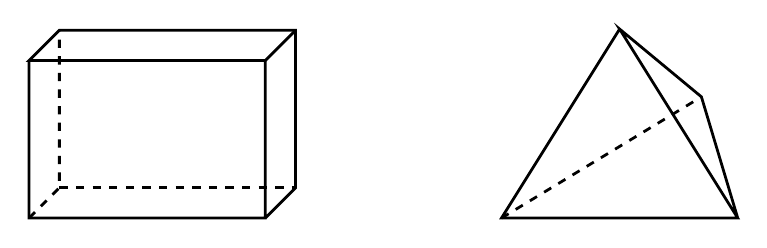
\begin{tikzpicture}[scale=2, line width=1pt]
\coordinate (A) at (0  ,0  ,0) ;
\coordinate (B) at (1.5,0  ,0) ;
\coordinate (C) at (1.5,1  ,0) ;
\coordinate (D) at (0  ,1  ,0) ;
\coordinate (E) at (0  ,0  ,-0.5) ;
\coordinate (F) at (1.5,0  ,-0.5) ;
\coordinate (G) at (1.5,1  ,-0.5) ;
\coordinate (H) at (0  ,1  ,-0.5) ;
\draw (D) -- (A) -- (B) -- (C) -- (D) -- (H) -- (G) -- (F) -- (B);
\draw (C) -- (G);
\draw [dashed] (A) -- (E) -- (H);
\draw [dashed] (E) -- (F);
\coordinate (I) at (3   ,0  ,0) ;
\coordinate (J) at (4.5 ,0  ,0) ;
\coordinate (K) at (3.75,1.2,0) ;
\coordinate (L) at (4   ,0.5,-0.7) ;
\draw[black] (K) -- (I) -- (J) -- (K) -- (L) -- (J) ;
\draw [dashed] (I) -- (L);
\end{tikzpicture}
\caption{3D allowed elements}
\label{3D_mesh}
\end{center}
\end{figure}
\end{itemize}

\textbf{Be carefull} non standard and hybrih meshing are not supported! (cf Figure \ref{hybr})

\begin{figure}[h!]
\begin{center}
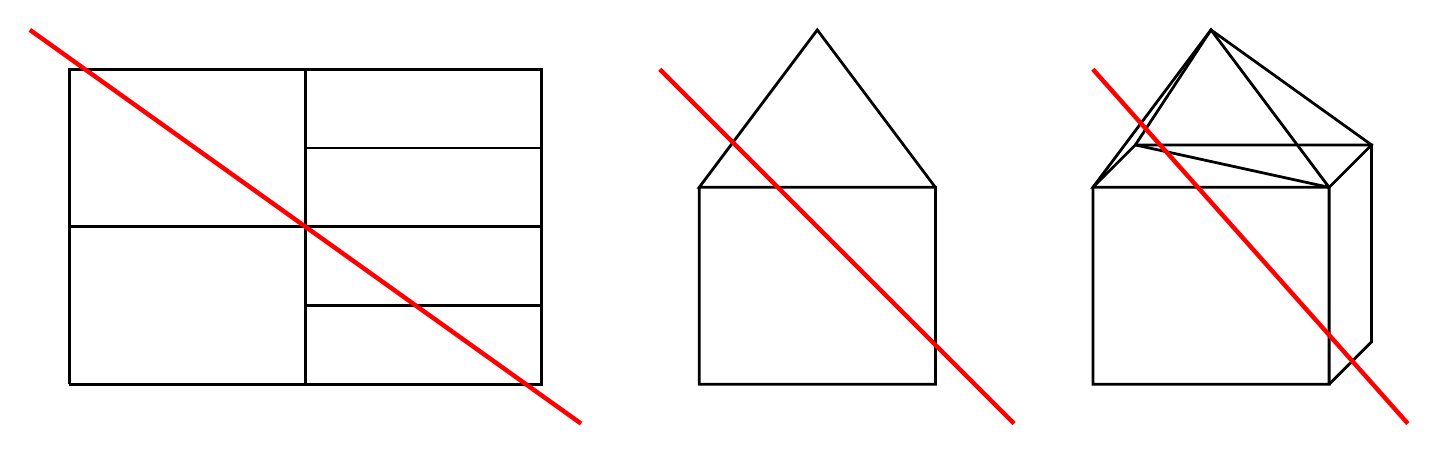
\begin{tikzpicture}[scale=2, line width=1pt]
\coordinate (A1) at (0,0) ;
\coordinate (A2) at (0,1) ;
\coordinate (A3) at (0,2) ;
\coordinate (B1) at (1.5,0  ) ;
\coordinate (B2) at (1.5,0.5) ;
\coordinate (B3) at (1.5,1  ) ;
\coordinate (B4) at (1.5,1.5) ;
\coordinate (B5) at (1.5,2  ) ;
\coordinate (C1) at (3,0  ) ;
\coordinate (C2) at (3,0.5) ;
\coordinate (C3) at (3,1  ) ;
\coordinate (C4) at (3,1.5) ;
\coordinate (C5) at (3,2  ) ;
\draw (A1) -- (C1) -- (C5) -- (A3) -- (A1);
\draw (A2) -- (C3);
\draw (B1) -- (B5);
\draw (B4) -- (C4);
\draw (B2) -- (C2);
\draw [ultra thick,red] (-0.25,2.25) -- (3.25,-0.25) ;

\coordinate (D1) at (4   ,0) ;
\coordinate (D2) at (5.5 ,0) ;
\coordinate (D3) at (5.5 ,1.25) ;
\coordinate (D4) at (4   ,1.25) ;
\coordinate (D5) at (4.75,2.25) ;
\draw (D4) -- (D1) -- (D2) -- (D3) -- (D4) -- (D5) -- (D3);
\draw [ultra thick,red] (3.75,2) -- (6,-0.25) ;

\coordinate (E1) at (6.5 ,0   ,0) ;
\coordinate (E2) at (8   ,0   ,0) ;
\coordinate (E3) at (8   ,1.25,0) ;
\coordinate (E4) at (6.5 ,1.25,0) ;
\coordinate (E5) at (7.25,2.25,0) ;
\coordinate (E6) at (8   ,0   ,-0.7) ;
\coordinate (E7) at (8   ,1.25,-0.7) ;
\coordinate (E8) at (6.5 ,1.25,-0.7) ;
\draw (E4) -- (E1) -- (E2) -- (E3) -- (E4) -- (E5) -- (E3);
\draw (E2) -- (E6) -- (E7) -- (E8) -- (E4);
\draw (E8) -- (E5) -- (E7) -- (E3) -- (E8);
\draw [ultra thick,red] (6.5,2) -- (8.5,-0.25) ;

\end{tikzpicture}
\caption{Prohibited meshes}
\label{hybr}
\end{center}
\end{figure}









%%%%%%%%%%%%%%%%%%%%%%%%%%%%%%%%%%%%%%
\subsection{Import mesh file}
%%%%%%%%%%%%%%%%%%%%%%%%%%%%%%%%%%%%%%
If your mesh was generated with an external tool like \href{http://www.salome-platform.org}{Salom\'e} (open source software), \href{http://resource.ansys.com/Products/Other+Products/ANSYS+ICEM+CFD}{ICEM} (commercial software), \href{http://gmsh.info/}{Gmsh} (open source software, included in \trust package) or \href{http://www-cast3m.cea.fr/}{Cast3M} (CEA software), then you must use one of the following keyword into your data file:

\begin{itemize}
\item \href{\REFERENCEMANUAL\#readmed}{\textbf{Read\_MED}} for a MED file from \href{http://www.salome-platform.org}{Salom\'e}, \href{http://gmsh.info/}{Gmsh},... ,
\item \href{\REFERENCEMANUAL\#readfile}{\textbf{Read\_File}} for a binary mesh file from \href{http://resource.ansys.com/Products/Other+Products/ANSYS+ICEM+CFD}{ICEM},
\item for another format, see the \href{\REFERENCEMANUAL\#read}{\trust Reference Manual}.
\end{itemize}

If you want to learn how to make a mesh with Salom\'e or Gmsh and read it with \trust, you can go to see the exercises of the \trust tutorial: \href{TRUST_tutorial.pdf\#salome}{here} for Salom\'e and \href{TRUST_tutorial.pdf\#gmsh}{here} for Gmsh.




%%%%%%%%%%%%%%%%%%%%%%%%%%%%%%%%%%%%%%
\subsection{Create quickly a mesh}
%%%%%%%%%%%%%%%%%%%%%%%%%%%%%%%%%%%%%%
Here is an example of a simple geometry (of non complex channel type) using the internal tool of \trust:
\begin{center}
\fbox{ \begin{minipage}[c]{0.9\textwidth}
\begin{alltt}
{\bf{Mailler}} \textit{my\_domain}

\{

\hspace{1cm}        \textcolor{blue}{/* Define the domain with one cavity */}

\hspace{1cm}        \textcolor{blue}{/* cavity 1m*2m with 5*22 cells */}

\hspace{1cm}        {\bf{Pave}} \textit{box}

\hspace{1cm}        \{

\hspace{2cm}            {\bf{Origine}} 0. 0.

\hspace{2cm}            {\bf{Longueurs}} 1 2

\hspace{2cm}            \textcolor{blue}{/* Cartesian grid */}

\hspace{2cm}            {\bf{Nombre\_de\_Noeuds}} 6 23

\hspace{2cm}            \textcolor{blue}{/* Uniform mesh */}

\hspace{2cm}            {\bf{Facteurs}} 1. 1.

\hspace{1cm}        \}

\hspace{1cm}        \{

\hspace{2cm}            \textcolor{blue}{/* Definition and names of boundary conditions */}

\hspace{2cm}            {\bf{bord}} \textit{Inlet}   \hspace{0.25cm} X = 0.  0. <= Y <= 2.

\hspace{2cm}            {\bf{bord}} \textit{Outlet}  \hspace{0.05cm} X = 1.  0. <= Y <= 2.

\hspace{2cm}            {\bf{bord}} \textit{Upper}   \hspace{0.25cm} Y = 2.  0. <= X <= 1.

\hspace{2cm}            {\bf{bord}} \textit{Lower}   \hspace{0.25cm} Y = 0.  0. <= X <= 1.

\hspace{1cm}        \}

\}
\end{alltt}
\end{minipage}}
\end{center}

To use this mesh in your data file, you just have to add the previous block in your data file or save it in a file named for example "\textit{my\_mesh.geo}" and add the line:\\
\begin{center}
\fbox{ \begin{minipage}[c]{0.5\textwidth}
\begin{alltt}
{\bf{Read\_file}} \textit{my\_mesh.geo} \textcolor{red}{{\bf{;}}}
\end{alltt}
\end{minipage}}
\end{center}

\underline{Do not forget the semi-colonn at the end of the line!}\\




%%%%%%%%%%%%%%%%%%%%%%%%%%%%%%%%%%%%%%
\subsection{Transform mesh within data file}
%%%%%%%%%%%%%%%%%%%%%%%%%%%%%%%%%%%%%%
You can also made transformations on your mesh after the \textbf{"Mailler"} or \textbf{"Read\_*"} command, using the following keywords:
\begin{itemize}
\item \href{\REFERENCEMANUAL\#triangulate}{\textbf{Trianguler}} to triangulate your 2D cells and create an unstructured mesh.
\item \href{\REFERENCEMANUAL\#tetraedriser}{\textbf{Tetraedriser}} to tetrahedralise 3D cells and create an unstructured mesh.
\item \href{\REFERENCEMANUAL\#raffineranisotrope}{\textbf{Raffiner\_anisotrope}}/\href{\REFERENCEMANUAL\#raffinerisotrope}{\textbf{Raffiner\_isotrope}} to triangulate/tetrahedralise elements of an untructured mesh.
\item \href{\REFERENCEMANUAL\#extrudebord}{\textbf{ExtrudeBord}} to generate an extruded mesh from a boundary of a tetrahedral or an hexahedral mesh. 
\Note that ExtrudeBord in VEF generates 3 or 14 tetrahedra from extruded prisms.
\item \href{\REFERENCEMANUAL\#regroupebord}{\textbf{RegroupeBord}} to build a new boundary with several boundaries of the domain.
\item \href{\REFERENCEMANUAL\#transformer}{\textbf{Transformer}} to transform the coordinates of the geometry.
\item for other commands, see the section \href{\REFERENCEMANUAL\#interprete}{interprete} of the \trust Reference Manual.
\end{itemize}

\Note that theses mesh modifications work on all mesh type (i.e. also for \textbf{*.geo} or \textbf{*.bin} or \textbf{*.med} files).



%%%%%%%%%%%%%%%%%%%%%%%%%%%%%%%%%%%%%%
\subsection{Test your mesh}
%%%%%%%%%%%%%%%%%%%%%%%%%%%%%%%%%%%%%%
The keyword \href{\REFERENCEMANUAL\#discretiserdomaine}{\textbf{Discretiser\_domaine}} is useful to discretize the domain (faces will be created) without defining a problem.
Indeed, you can create a minimal data file, post-process your mesh in lata format (for example) and visualize it with VisIt. \\

\Note that you must name all the boundaries!\\

Here is an example of this kind of data file:

\begin{center}
\fbox{ \begin{minipage}[c]{0.8\textwidth}
\begin{center}
\textbf{my\_data\_file.data}
\end{center}
\end{minipage}}
\fbox{ \begin{minipage}[c]{0.8\textwidth}
\begin{alltt}
{\bf{dimension 3}}

{\bf{Domaine}} \textit{my\_domain}

{\bf{Mailler}} \textit{my\_domain}

\{

\hspace{1cm}    {\bf{Pave}} \textit{box}

\hspace{1cm}    \{

\hspace{2cm}        {\bf{Origine}} 0. 0. 0.

\hspace{2cm}        {\bf{Longueurs}} 1 2 1

\hspace{2cm}        {\bf{Nombre\_de\_Noeuds}} 6 23 6

\hspace{2cm}        {\bf{Facteurs}} 1. 1. 1.

\hspace{1cm}    \}

\hspace{1cm}    \{

\hspace{2cm}        {\bf{bord}} \textit{Inlet}  \hspace{0.25cm} X = 0. 0. <= Y <= 2.  0. <= Z <= 1.

\hspace{2cm}        {\bf{bord}} \textit{Outlet} \hspace{0.05cm} X = 1.  0. <= Y <= 2.  0. <= Z <= 1.

\hspace{2cm}        {\bf{bord}} \textit{Upper}  \hspace{0.25cm} Y = 2.  0. <= X <= 1.  0. <= Z <= 1.

\hspace{2cm}        {\bf{bord}} \textit{Lower}  \hspace{0.25cm} Y = 0. 0. <= X <= 1.  0. <= Z <= 1.

\hspace{2cm}        {\bf{bord}} \textit{Front}  \hspace{0.25cm} Z = 0. 0. <= X <= 1.  0. <= Y <= 2.

\hspace{2cm}        {\bf{bord}} \textit{Back}   \hspace{0.45cm} Z = 1. 0. <= X <= 1.  0. <= Y <= 2.

\hspace{1cm}    \}

\}

{\bf{discretiser\_domaine}} \textit{my\_domain}

{\bf{postraiter\_domaine}} \{ {\bf{domaine}} \textit{my\_domain} {\bf{format lata}} \}

{\bf{End}}
    \end{alltt}
\end{minipage}}
\end{center}

To use it, launch in a bash terminal:
\begin{verbatim}
# if not already done
> source $my_path_to_TRUST_installation/env_TRUST.sh
# then
> trust my_data_file
> visit -o my_data_file.lata &
\end{verbatim}

To see how to use VisIt, go to see the first \trust tutorial exercise: \href{TRUST_tutorial.pdf\#exo1}{Obstacle}.\\

If you want to learn how to make a mesh with Salom\'e or Gmsh and read it with \trust, you can go to see the exercises of the \trust tutorial: \href{TRUST_tutorial.pdf\#salome}{here} for Salom\'e and \href{TRUST_tutorial.pdf\#gmsh}{here} for Gmsh.







%%%%%%%%%%%%%%%%%%%%%%%%%%%%%%%%%%%%%%%%%%%%%%%%%%%%%%%%%%%%%%%
\section{Discretization}
%%%%%%%%%%%%%%%%%%%%%%%%%%%%%%%%%%%%%%%%%%%%%%%%%%%%%%%%%%%%%%%
You have to specify the discretization type which can be \href{\REFERENCEMANUAL\#vdf}{\textbf{VDF}}, \href{\REFERENCEMANUAL\#ef}{\textbf{EF}} or \href{\REFERENCEMANUAL\#vefprep1b}{\textbf{VEFPreP1B}}.\\

In \textbf{VDF} discretization, the locations of the unknown are drawn in the Figure \ref{fig_VDF}.\\

\begin{figure}[h!]
\begin{center}
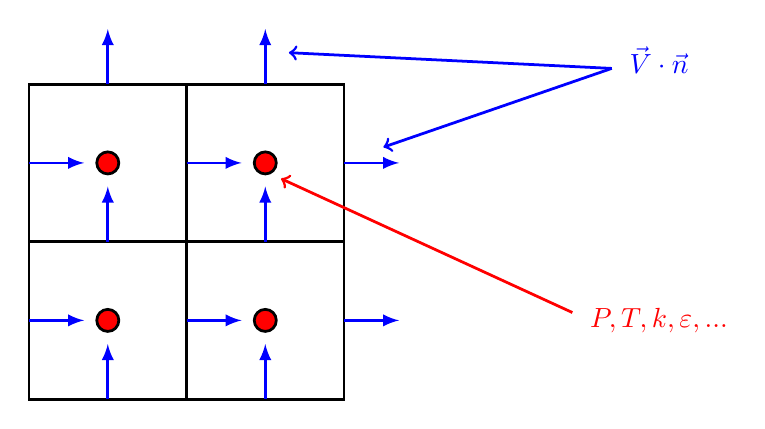
\begin{tikzpicture}[scale=2, line width=1pt]
\coordinate (A) at (0,0) ;
\coordinate (B) at (1,0) ;
\coordinate (C) at (2,0) ;
\coordinate (D) at (2,1) ;
\coordinate (E) at (2,2) ;
\coordinate (F) at (1,2) ;
\coordinate (G) at (0,2) ;
\coordinate (H) at (0,1) ;
\draw[black] (A) -- (C) -- (E) -- (G) -- cycle ;
\draw[black] (H) -- (D) ;
\draw[black] (F) -- (B) ;
\draw[black,fill=red] (0.5,0.5) circle (0.07);
\draw[black,fill=red] (1.5,0.5) circle (0.07);
\draw[black,fill=red] (0.5,1.5) circle (0.07);
\draw[black,fill=red] (1.5,1.5) circle (0.07);
\draw[blue] [->] [>=latex] (0.5,0) -- (0.5,0.35);
\draw[blue] [->] [>=latex] (0.5,1) -- (0.5,1.35);
\draw[blue] [->] [>=latex] (0.5,2) -- (0.5,2.35);
\draw[blue] [->] [>=latex] (1.5,0) -- (1.5,0.35);
\draw[blue] [->] [>=latex] (1.5,1) -- (1.5,1.35);
\draw[blue] [->] [>=latex] (1.5,2) -- (1.5,2.35);
\draw[blue] [->] [>=latex] (0,0.5) -- (0.35,0.5);
\draw[blue] [->] [>=latex] (1,0.5) -- (1.35,0.5);
\draw[blue] [->] [>=latex] (2,0.5) -- (2.35,0.5);
\draw[blue] [->] [>=latex] (0,1.5) -- (0.35,1.5);
\draw[blue] [->] [>=latex] (1,1.5) -- (1.35,1.5);
\draw[blue] [->] [>=latex] (2,1.5) -- (2.35,1.5);
\draw[blue] (4,2) node[above]{$\vec{V} \cdot \vec{n}$} ;
\draw[blue] [<-] (1.65,2.2) -- (3.7,2.1);
\draw[blue] [<-] (2.25,1.6) -- (3.7,2.1);
\draw[red] (4,0.5) node {$P, T, k, \varepsilon, ...$} ;
\draw[red] [<-] (1.6,1.4) -- (3.45,0.55);
\end{tikzpicture}
\caption{VDF unknown localisations}
\label{fig_VDF}
\end{center}
\end{figure}

For \textbf{VEFPreP1B}, the locations of the unknown are drawn in the Figure \ref{fig_VEF}.\\

\begin{figure}[h!]
\begin{center}
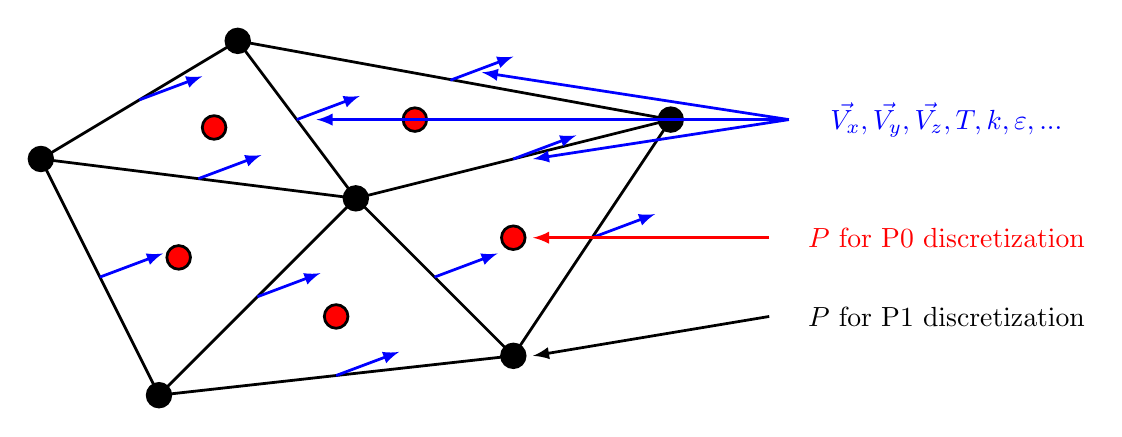
\begin{tikzpicture}[scale=1, line width=1pt]
\coordinate (A) at (1.5,0) ;
\coordinate (B) at (6,0.5) ;
\coordinate (C) at (8,3.5) ;
\coordinate (D) at (2.5,4.5) ;
\coordinate (E) at (0,3) ;
\coordinate (F) at (4,2.5) ;
\draw[black] (A) -- (B) -- (C) -- (D) -- (E) -- (A) -- (F) -- (B);
\draw[black] (C) -- (F) -- (D);
\draw[black] (E) -- (F);
\draw[black,fill=black] (A) circle (0.15);
\draw[black,fill=black] (B) circle (0.15);
\draw[black,fill=black] (C) circle (0.15);
\draw[black,fill=black] (D) circle (0.15);
\draw[black,fill=black] (E) circle (0.15);
\draw[black,fill=black] (F) circle (0.15);
\draw[black,fill=red] (3.75,1) circle (0.15);
\draw[black,fill=red] (6,2) circle (0.15);
\draw[black,fill=red] (4.75,3.5) circle (0.15);
\draw[black,fill=red] (2.2,3.4) circle (0.15);
\draw[black,fill=red] (1.75,1.75) circle (0.15);
\begin{scope}[xshift=5cm, yshift=1.5cm]
\draw[blue] [->] [>=latex] (0,0) -- (0.8,0.3);
\end{scope}
\begin{scope}[xshift=7cm, yshift=2cm]
\draw[blue] [->] [>=latex] (0,0) -- (0.8,0.3);
\end{scope}
\begin{scope}[xshift=5.2cm, yshift=4cm]
\draw[blue] [->] [>=latex] (0,0) -- (0.8,0.3);
\end{scope}
\begin{scope}[xshift=1.25cm, yshift=3.75cm]
\draw[blue] [->] [>=latex] (0,0) -- (0.8,0.3);
\end{scope}
\begin{scope}[xshift=0.75cm, yshift=1.5cm]
\draw[blue] [->] [>=latex] (0,0) -- (0.8,0.3);
\end{scope}
\begin{scope}[xshift=2.75cm, yshift=1.25cm]
\draw[blue] [->] [>=latex] (0,0) -- (0.8,0.3);
\end{scope}
\begin{scope}[xshift=3.75cm, yshift=0.25cm]
\draw[blue] [->] [>=latex] (0,0) -- (0.8,0.3);
\end{scope}
\begin{scope}[xshift=6cm, yshift=3cm]
\draw[blue] [->] [>=latex] (0,0) -- (0.8,0.3);
\end{scope}
\begin{scope}[xshift=3.25cm, yshift=3.5cm]
\draw[blue] [->] [>=latex] (0,0) -- (0.8,0.3);
\end{scope}
\begin{scope}[xshift=2cm, yshift=2.75cm]
\draw[blue] [->] [>=latex] (0,0) -- (0.8,0.3);
\end{scope}
\draw[blue] (11.5,3.5) node {$\vec{V_x}, \vec{V_y}, \vec{V_z}, T, k, \varepsilon, ...$} ;
\draw[blue] [->] [>=latex] (9.5,3.5) -- (5.6,4.1);
\draw[blue] [->] [>=latex] (9.5,3.5) -- (3.5,3.5);
\draw[blue] [->] [>=latex] (9.5,3.5) -- (6.25,3);
\draw[red] (11.5,2) node {$P$ for P0 discretization} ;
\draw[red] [->] [>=latex] (9.25,2) -- (6.25,2);
\draw[black] (11.5,1) node {$P$ for P1 discretization} ;
\draw[black] [->] [>=latex] (9.25,1) -- (6.25,0.5);
\end{tikzpicture}
\caption{VEF unknown localisations in 2D}
\label{fig_VEF}
\end{center}
\end{figure}

In 3D for the pressure, we can also use the P0+P1+Pa discretization for flow with a strong source term and a low velocity field.
In this case P0+P1 pressure gradient has trouble to match the source term so we use P0+P1+Pa discretization (cf Figure \ref{fig_VEF_pressure_loc}).

\begin{figure}[h!]
\begin{center}
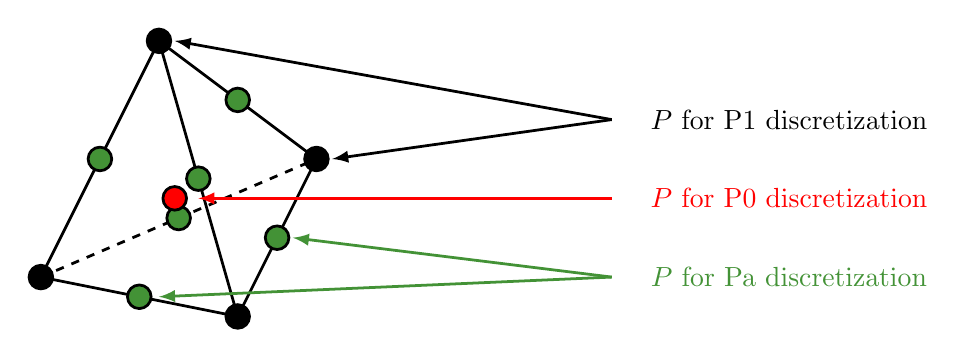
\begin{tikzpicture}[scale=1, line width=1pt]
\coordinate (A) at (0.5,1) ;
\coordinate (B) at (3,0.5) ;
\coordinate (C) at (4,2.5) ;
\coordinate (D) at (2,4) ;
\draw[black] (B) -- (C) -- (D) -- (A) -- (B) -- (D);
\draw[black,dashed] (A) -- (C);
\draw[black,fill=black] (A) circle (0.15);
\draw[black,fill=black] (B) circle (0.15);
\draw[black,fill=black] (C) circle (0.15);
\draw[black,fill=black] (D) circle (0.15);
\draw[black,fill=Greeen] (1.75,0.75) circle (0.15);
\draw[black,fill=Greeen] (3.5,1.5) circle (0.15);
\draw[black,fill=Greeen] (3,3.25) circle (0.15);
\draw[black,fill=Greeen] (1.25,2.5) circle (0.15);
\draw[black,fill=Greeen] (2.25,1.75) circle (0.15);
\draw[black,fill=Greeen] (2.5,2.25) circle (0.15);
\draw[black,fill=red] (2.2,2) circle (0.15);
\draw[black] (10,3) node {$P$ for P1 discretization} ;
\draw[black] [->] [>=latex] (7.75,3) -- (2.2,4);
\draw[black] [->] [>=latex] (7.75,3) -- (4.2,2.5);
\draw[red] (10,2) node {$P$ for P0 discretization} ;
\draw[red] [->] [>=latex] (7.75,2) -- (2.5,2);
\draw[Greeen] (10,1) node {$P$ for Pa discretization} ;
\draw[Greeen] [->] [>=latex] (7.75,1) -- (3.7,1.5);
\draw[Greeen] [->] [>=latex] (7.75,1) -- (2,0.75);
\end{tikzpicture}
\caption{VEF pressure localisation in 3D}
\label{fig_VEF_pressure_loc}
\end{center}
\end{figure}

To specify the wanted discretization, you have to add the following block to your data file:

    \begin{center}
    \fbox{ \begin{minipage}[c]{0.5\textwidth}
    \begin{alltt}
    \textit{{\bf{Discretization\_type}} my\_discretization}

    [{\bf{Read }} \textit{my\_discretization \{ ... \}}]
    \end{alltt}
    \end{minipage}}
    \end{center}

You can add parameters to your discretization with the optional keyword \href{\REFERENCEMANUAL\#read}{\textbf{Read}} (see \href{\REFERENCEMANUAL\#vefprep1b}{\textbf{VEFPreP1B discretization}}).

On the \href{http://www-trio-u.cea.fr/scripts/home/publigen/content/templates/show.asp?L=EN&P=55&vTicker=alleza&ITEMID=3}{TRUST website}, you can find information about:
\begin{itemize}
\item \textbf{VDF} discretization in the \href{http://www-trio-u.cea.fr/home/liblocal/docs/Theses/these_chatelain_2004.pdf}{PhD thesis of A. Chatelain},
\item \textbf{VEFPreP1B} discretization (Crouzet-Raviart elements) in the \href{http://www-trio-u.cea.fr/home/liblocal/docs/Theses/these_fortin_2006.pdf}{PhD thesis of T. Fortin} and \href{http://www-trio-u.cea.fr/home/liblocal/docs/Theses/These_Heib_2003.pdf}{PhD thesis of S. Heib}.
\end{itemize}


%%%%%%%%%%%%%%%%%%%%%%%%%%%%%%%%%%%%%%%%%%%%%%%%%%%%%%%%%%%%%%%
\section{Time schemes}
%%%%%%%%%%%%%%%%%%%%%%%%%%%%%%%%%%%%%%%%%%%%%%%%%%%%%%%%%%%%%%%
Now you can choose your time scheme to solve your problem. For this you must
specify the time scheme type wanted and give it a name. 
then you have to specify its parameters by filling the associated \textbf{"Read"} block.

    \begin{center}
    \fbox{ \begin{minipage}[c]{0.5\textwidth}
    \begin{alltt}
    {\bf{\textit{Scheme\_type}}} \textit{my\_time\_scheme}

    {\bf{Read}} \textit{my\_time\_scheme} \{ ... \}
    \end{alltt}
    \end{minipage}}
    \end{center}

%%%%%%%%%%%%%%%%%%%%%%%%%%%%%%%%%%%%%%
\subsection{Some available time schemes}
%%%%%%%%%%%%%%%%%%%%%%%%%%%%%%%%%%%%%%
%Here are some \href[page=DOCLINK_TIME SCHEMES]{\REFERENCEMANUAL}{available types of explicit schemes}:
Here are some available types of explicit schemes:
\begin{itemize}
\item \href{\REFERENCEMANUAL\#eulerscheme}{\textbf{Scheme\_Euler\_explicit}},
\item \href{\REFERENCEMANUAL\#schemaadamsbashforthorder2}{\textbf{Schema\_Adams\_Bashforth\_order\_2}},
%\item \textbf{Schema\_Adams\_Bashforth\_order\_3}
%\item \textbf{Runge\_Kutta\_Rationnel\_ordre\_2}
\item \href{\REFERENCEMANUAL\#rungekuttaordre3}{\textbf{Runge\_Kutta\_ordre\_3}},
%\item \textbf{Runge\_Kutta\_ordre\_4\_D3P}
%\item \textbf{Schema\_Predictor\_Corrector}
%\item \textbf{Sch\_CN\_iteratif}
%\item \textbf{Sch\_CN\_EX\_iteratif}
%\item \textbf{Schema\_Phase\_Field}
%\item \textbf{RK3\_FT}
\end{itemize}

%And also some \href[page=DOCLINK_TIME SCHEMES]{\REFERENCEMANUAL}{available types of implicit schemes}:
And also some available types of implicit schemes:
\begin{itemize}
\item \href{\REFERENCEMANUAL\#schemaeulerimplicite}{\textbf{Scheme\_Euler\_implicit}},
%\item \textbf{Schema\_Adams\_Moulton\_order\_2}
\item \href{\REFERENCEMANUAL\#schemaadamsmoultonorder3}{\textbf{Schema\_Adams\_Moulton\_order\_3}}.
%\item \textbf{Schema\_Backward\_Differentiation\_order\_2}
%\item \textbf{Schema\_Backward\_Differentiation\_order\_3}
\end{itemize}

For other scheme, see \href{\REFERENCEMANUAL\#schematempsbase}{this section} of the Reference Manual.\\

\Note that you can use semi-implicit schemes activating the \textbf{diffusion\_implicite} keyword in your explicit time scheme.



%%%%%%%%%%%%%%%%%%%%%%%%%%%%%%%%%%%%%%
\subsection{Calculation stopping condition}
%%%%%%%%%%%%%%%%%%%%%%%%%%%%%%%%%%%%%%
You must specify at least one stopping condition for you simulation.
It can be:
\begin{itemize}
\item the final time: \textbf{tmax}
\item the maximal allowed cpu time: \textbf{tcpumax}
\item the number of time step: \textbf{nb\_pas\_dt\_max}
\item the convergency treshold: \textbf{seuil\_statio}
\end{itemize}

\Note that if the time step wants to go under the minimal time step \textbf{dt\_min}, \trust will stop the calculation.\\

If you want to stop properly your running calculation (i.e. with all saves), you may use the \textit{my\_data\_file}.stop file (cf section \ref{stopfile}).
When the simulation is running, you can see the "\textbf{0}" value in that file.\\

To stop it, put a "\textbf{1}" instead of the "\textbf{0}" and at the next iteration the calculation will stop properly.\\

When you don't change any thing to that file, at the end of the calculation, you can see that it is writen "\textbf{Finished correctly}".


%%%%%%%%%%%%%%%%%%%%%%%%%%%%%%%%%%%%%%%%%%%%%%%%%%%%%%%%%%%%%%%
\section{Medium/Type of fluide}
%%%%%%%%%%%%%%%%%%%%%%%%%%%%%%%%%%%%%%%%%%%%%%%%%%%%%%%%%%%%%%%
To specify the medium or fluid, you may add the following block.

    \begin{center}
    \fbox{ \begin{minipage}[c]{0.5\textwidth}
    \begin{alltt}
    {\bf{\textit{Fluid\_type}}} \textit{my\_medium}

    {\bf{Read}} \textit{my\_medium} \{ ... \}
    \end{alltt}
    \end{minipage}}
    \end{center}

{\bf{\textit{Fluid\_type}}} can be one of the following:
\begin{itemize}
\item \href{\REFERENCEMANUAL\#fluideincompressible}{\textbf{Fluide\_incompressible}}
\item \href{\REFERENCEMANUAL\#fluidequasicompressible}{\textbf{Fluide\_quasi\_compressible}}
%\item \textbf{Fluide\_Ostwald}
%\item \textbf{Constituant}
\item \href{\REFERENCEMANUAL\#solide}{\textbf{Solide}}
\item for other types and more information see \href{\REFERENCEMANUAL\#milieubase}{\trust Reference Manual}.
\end{itemize}

If you want to use more than one medium, you can add an other block for each medium or fluid.\\





%%%%%%%%%%%%%%%%%%%%%%%%%%%%%%%%%%%%%%%%%%%%%%%%%%%%%%%%%%%%%%%
\section{Add gravity}
%%%%%%%%%%%%%%%%%%%%%%%%%%%%%%%%%%%%%%%%%%%%%%%%%%%%%%%%%%%%%%%
If needed, you can add gravity term to your simulation. This is done by adding
a uniform field, no matter his name. For example in 2D:

    \begin{center}
    \fbox{ \begin{minipage}[c]{0.5\textwidth}
    \begin{alltt}
    \textcolor{blue}{\# Gavity vector definition \#}

    {\bf{Uniform\_field}} \textit{my\_gravity}

    {\bf{Read}} \textit{my\_gravity 2 0 -9.81}

    \end{alltt}
    \end{minipage}}
    \end{center}




%%%%%%%%%%%%%%%%%%%%%%%%%%%%%%%%%%%%%%%%%%%%%%%%%%%%%%%%%%%%%%%
\section{Objects association and discretization}
%%%%%%%%%%%%%%%%%%%%%%%%%%%%%%%%%%%%%%%%%%%%%%%%%%%%%%%%%%%%%%%
%%%%%%%%%%%%%%%%%%%%%%%%%%%%%%%%%%%%%%
\subsection{Association}
%%%%%%%%%%%%%%%%%%%%%%%%%%%%%%%%%%%%%%
Until now, we have created some objects, now we must associate them together.
For this, we must use the \href{\REFERENCEMANUAL\#associate}{\textbf{Associate}} interpretor:
    \begin{center}
    \fbox{ \begin{minipage}[c]{0.7\textwidth}
    \begin{alltt}
    \textcolor{blue}{\# Association between the different objects \#}

    {\bf{Associate}} \textit{my\_problem my\_domain}

    {\bf{Associate}} \textit{my\_problem my\_time\_scheme}

    {\bf{Associate}} \textit{my\_problem my\_medium}

    [{\bf{Associate}} \textit{my\_medium my\_gravity}]
    \end{alltt}
    \end{minipage}}
    \end{center}




%%%%%%%%%%%%%%%%%%%%%%%%%%%%%%%%%%%%%%
\subsection{Discretization}
%%%%%%%%%%%%%%%%%%%%%%%%%%%%%%%%%%%%%%
Then you must discretize your domain using the \href{\REFERENCEMANUAL\#discretize}{\textbf{Discretize}} interpretor:
    \begin{center}
    \fbox{ \begin{minipage}[c]{0.7\textwidth}
    \begin{alltt}
    {\bf{Discretize}}  \textit{my\_problem  my\_discretization}
    \end{alltt}
    \end{minipage}}
    \end{center}

The problem \textit{my\_problem} is discretized according to the \textit{my\_discretization} discretization.\\

IMPORTANT: A number of objects must be already associated (a domain, time scheme, central object) prior to invoking the \textbf{Discretize} keyword. The physical properties of this central object must also have been read.\\

\Note that when \trust succed the discretization step, the mesh is then validated by the code.\\

At this level of your data file, you can visualize your mesh with the "\textbf{-mesh}" option of the trust script, it will directly open your mesh with VisIt.
\begin{verbatim}
# if not already done
> source $my_path_to_TRUST_installation/env_TRUST.sh
# then
> trust -mesh my_data_file
\end{verbatim}
It will only run the mesh and stop, the problem will not be solved.




%%%%%%%%%%%%%%%%%%%%%%%%%%%%%%%%%%%%%%%%%%%%%%%%%%%%%%%%%%%%%%%%%%%%%%%%



%%%%%%%%%%%%%%%%%%%%%%%%%%%%%%%%%%%%%%%%%%%%%%%%%%%%%%%%%%%%%%%%%%%%%%%%
%
\chapter{Problem definition}
%
%%%%%%%%%%%%%%%%%%%%%%%%%%%%%%%%%%%%%%%%%%%%%%%%%%%%%%%%%%%%%%%%%%%%%%%%
%%%%%%%%%%%%%%%%%%%%%%%%%%%%%%%%%%%%%%%%%
\section{Set of equations}
%%%%%%%%%%%%%%%%%%%%%%%%%%%%%%%%%%%%%%%%%
In function of your choice of problem type, you will have a different set of equations.

%%%%%%%%%%%%%%%%%%%%%%%%%%%%%%%%%%%%%%
\subsection{Incompressible problems}
%%%%%%%%%%%%%%%%%%%%%%%%%%%%%%%%%%%%%%
\trust solves Navier-Stokes equations with/without heat equation for incompressible fluid:

$$
\left\{
\begin{array}{c}
\nabla \cdot \vec u =0 \\
\displaystyle{\frac{\partial \vec u }{\partial t} + \textcolor{red}{\nabla \cdot (\vec u \otimes \vec u)} = \textcolor{blue}{\nabla \cdot (\nu \nabla \vec u)} - \nabla P^* } \\
\displaystyle{\frac{\partial T}{\partial t} + \textcolor{red}{\vec u \nabla T} = \textcolor{blue}{\nabla \cdot (\alpha \nabla T)} + \frac{Q}{\rho C_p}}
\end{array}
\right.
$$

where: $\displaystyle{P^*=\frac{P}{\rho} + g z}$, $Q$ is a heat source term, and:

\begin{itemize}
\item $\rho$: density,
\item $\mu$: dynamic viscosity,
\item $\displaystyle{\nu=\frac{\mu}{\rho}}$: cinematic viscosity,
\item $\vec g=g z$: gravity vector in cartesian coordinates,
\item $\displaystyle{\alpha=\frac{\lambda}{\rho C_p}}$: thermal diffusivity.
\item $C_p$: specific heat capacity at constant pressure,
\item $\lambda$: thermal conductivity,
\end{itemize}

\Note that \textcolor{red}{red} terms are convective terms and \textcolor{blue}{blue} terms are diffusive terms.\\

\begin{center}
\fbox{ \begin{minipage}[c]{0.98\textwidth}
\begin{alltt}
{\bf{Pb\_\textcolor{magenta}{Thermo}hydraulique\textcolor{darkblue}{\_Concentration}\hspace{-0.15cm}\textcolor{Greeen}{\_Turbulent} } } \textit{my\_problem}

...

{\bf{Read}} \textit{my\_problem}

\{

\hspace{1cm}    \textcolor{blue}{\# Navier Stokes equations with/without turbulent model \#}

\hspace{1cm}    {\bf{Navier\_Stokes$\overbrace{\mbox{\_Standard}}^{\mbox{\textcolor{Greeen}{\_Turbulent}}}$} }

\hspace{1cm}    \{

\hspace{2cm}        {\bf{Solveur\_Pression}} \textit{my\_solver} \{ ... \}

\hspace{2cm}        {\bf{Diffusion}} \{ ... \}

\hspace{2cm}        {\bf{Convection}} \{ ... \}

\hspace{2cm}        {\bf{Initial\_conditions}} \{ ... \}

\hspace{2cm}        {\bf{Boundary\_conditions}} \{ ... \}

\hspace{2cm}        {\bf{\textcolor{Greeen}{Modele\_turbulence \textit{modele} \{ ... \} } }}

\hspace{2cm}        [{\bf{Sources}} \{ ... \}]

\hspace{2cm}       ...

\hspace{1cm}    \}

\hspace{1cm}    \textcolor{blue}{\# Energy equation with/without turbulent model \#}

\hspace{1cm}    {\bf{\textcolor{magenta}{Convection\_Diffusion\_Temperature}\textcolor{Greeen}{\_Turbulent}}}

\hspace{1cm}    \textcolor{magenta}{\{}

\hspace{2cm}        \textcolor{magenta}{{\bf{Diffusion}} \{ ... \}}

\hspace{2cm}        \textcolor{magenta}{{\bf{Convection}} \{ ... \}}

\hspace{2cm}        \textcolor{magenta}{{\bf{Initial\_conditions}} \{ ... \}}

\hspace{2cm}        \textcolor{magenta}{{\bf{Boundary\_conditions}} \{ ... \}}

\hspace{2cm}        \textcolor{magenta}{{\bf{\textcolor{Greeen}{Modele\_turbulence Prandtl \{ ... \} } }}}

\hspace{2cm}        \textcolor{magenta}{[{\bf{Sources}} \{ ... \}]}

\hspace{2cm}        \textcolor{magenta}{...}

\hspace{1cm}    \textcolor{magenta}{\}}

\hspace{1cm}    \textcolor{blue}{\# Constituent transportation equations with/without turbulent model \#}

\hspace{1cm}    {\bf{\textcolor{darkblue}{Convection\_Diffusion\_Concentration}\textcolor{Greeen}{\_Turbulent}}}

\hspace{1cm}    \textcolor{darkblue}{\{}

\hspace{2cm}        \textcolor{darkblue}{{\bf{Diffusion}} \{ ... \}}

\hspace{2cm}        \textcolor{darkblue}{{\bf{Convection}} \{ ... \}}

\hspace{2cm}        \textcolor{darkblue}{{\bf{Initial\_conditions}} \{ ... \}}

\hspace{2cm}        \textcolor{darkblue}{{\bf{Boundary\_conditions}} \{ ... \}}

\hspace{2cm}        \textcolor{darkblue}{{\bf{\textcolor{Greeen}{Modele\_turbulence Schmidt \{ ... \} } }}}

\hspace{2cm}        \textcolor{darkblue}{[{\bf{Sources}} \{ ... \}]}

\hspace{2cm}        \textcolor{darkblue}{...}

\hspace{1cm}    \textcolor{darkblue}{\}}

\}
\end{alltt}
\end{minipage}}
\end{center}

For documentation, see:\\

\begin{longtable}{|c|c|c|c|c|}
\hline
Thermo & hydraulique & Concentration & Turbulent & Reference Manual\tabularnewline
\hline 
\hline 
            & \textbf{Pb\_hydraulique}  &   
            &                           & \href{../../Outils/TRIOXDATA/XTriou/doc.pdf\#pbhydraulique}{doc} \tabularnewline 
\hline
            & \textbf{Pb\_hydraulique}  & \textbf{\textcolor{darkblue}{\_Concentration}}
            &                           & \href{../../Outils/TRIOXDATA/XTriou/doc.pdf\#pbhydrauliqueconcentration}{doc} \tabularnewline
\hline
            & \textbf{Pb\_hydraulique}  &   
            & \textbf{\textcolor{Greeen}{\_Turbulent}}      & \href{../../Outils/TRIOXDATA/XTriou/doc.pdf\#pbhydrauliqueturbulent}{doc} \tabularnewline
\hline
            & \textbf{Pb\_hydraulique}  & \textbf{\textcolor{darkblue}{\_Concentration}}
            & \textbf{\textcolor{Greeen}{\_Turbulent}}      & \href{../../Outils/TRIOXDATA/XTriou/doc.pdf\#pbhydrauliqueconcentrationturbulent}{doc} \tabularnewline
\hline
\textbf{Pb\_\textcolor{magenta}{Thermo}}     & \textbf{hydraulique}  &   
                        &                       & \href{../../Outils/TRIOXDATA/XTriou/doc.pdf\#pbthermohydraulique}{doc} \tabularnewline
\hline
\textbf{Pb\_\textcolor{magenta}{Thermo}}     & \textbf{hydraulique}  & \textbf{\textcolor{darkblue}{\_Concentration}}
                        &                       & \href{../../Outils/TRIOXDATA/XTriou/doc.pdf\#pbthermohydrauliqueconcentration}{doc} \tabularnewline
\hline
\textbf{Pb\_\textcolor{magenta}{Thermo}}     & \textbf{hydraulique}  &   
                        & \textbf{\textcolor{Greeen}{\_Turbulent}}  & \href{../../Outils/TRIOXDATA/XTriou/doc.pdf\#pbthermohydrauliqueturbulent}{doc} \tabularnewline
\hline
\textbf{Pb\_\textcolor{magenta}{Thermo}}     & \textbf{hydraulique}  & \textbf{\textcolor{darkblue}{\_Concentration}}
                        & \textbf{\textcolor{Greeen}{\_Turbulent}}  & \href{../../Outils/TRIOXDATA/XTriou/doc.pdf\#pbthermohydrauliqueconcentrationturbulent}{doc} \tabularnewline
\hline
\end{longtable}

\vspace{0.5cm}


%%%%%%%%%%%%%%%%%%%%%%%%%%%%%%%%%%%%%%
\subsection{Quasi-compressible problem}
%%%%%%%%%%%%%%%%%%%%%%%%%%%%%%%%%%%%%%
\trust solves Navier-Stokes equations with/without heat equation for quasi-compressible fluid:

$$
\left\{
\begin{array}{c}
\displaystyle{\frac{\partial \rho }{\partial t} + \nabla \cdot (\rho \vec u) =0 }\\
\displaystyle{ \frac{\partial \rho u}{\partial t} + \textcolor{red}{\nabla \cdot (\rho u u)} =  \textcolor{blue}{\nabla \cdot \left(\mu \nabla \vec u \right)} - \nabla P -\rho \vec g }\\
\displaystyle{ \rho C_p \left( \frac{\partial T}{\partial t} + \textcolor{red}{\vec u \nabla T} \right) = \textcolor{blue}{\nabla \cdot \left(\lambda \nabla T\right)} + \frac{dP_0}{dt} + Q }
\end{array}
\right.
$$

where: $P_0=\rho R T$, $Q$ is a heat source term, and:

\begin{itemize}
\item $\rho$: density,
\item $\mu$: dynamic viscosity,
\item $\displaystyle{\nu=\frac{\mu}{\rho}}$: cinematic viscosity,
\item $\vec g=g z$: gravity vector in cartesian coordinates,
\item $C_p$: specific heat capacity at constant pressure,
\item $\lambda$: thermal conductivity,
\item $\displaystyle{\alpha=\frac{\lambda}{\rho C_p}}$: thermal diffusivity.
\end{itemize}

\Note that \textcolor{red}{red} terms are convective terms and \textcolor{blue}{blue} terms are diffusive terms.\\


\begin{center}
\fbox{ \begin{minipage}[c]{0.95\textwidth}
\begin{alltt}
{\bf{Pb\_Thermohydraulique\textcolor{Greeen}{\_Turbulent}\_QC} } \textit{my\_problem}

...

{\bf{Read}} \textit{my\_problem}

\{

\hspace{1cm}    \textcolor{blue}{\# Navier Stokes equations for quasi-compressible fluid under \#}

\hspace{1cm}    \textcolor{blue}{\# low Mach numbers with/without turbulent model \#}

\hspace{1cm}    {\bf{Navier\_Stokes\textcolor{Greeen}{\_Turbulent}\_QC}}

\hspace{1cm}    \{

\hspace{2cm}        {\bf{Solveur\_Pression}} \textit{my\_solver} \{ ... \}

\hspace{2cm}        {\bf{Diffusion}} \{ ... \}

\hspace{2cm}        {\bf{Convection}} \{ ... \}

\hspace{2cm}        {\bf{Initial\_conditions}} \{ ... \}

\hspace{2cm}        {\bf{Boundary\_conditions}} \{ ... \}

\hspace{2cm}        {\bf{\textcolor{Greeen}{Modele\_turbulence \textit{modele} \{ ... \} } }}

\hspace{2cm}        [{\bf{Sources}} \{ ... \}]

\hspace{2cm}       ...

\hspace{1cm}    \}

\hspace{1cm}    \textcolor{blue}{\# Energy equation for quasi-compressible fluid under low Mach \#}

\hspace{1cm}    \textcolor{blue}{\# numbers with/without turbulent model \#}

\hspace{1cm}    {\bf{Convection\_Diffusion\_Chaleur}\textcolor{Greeen}{\_Turbulent}}

\hspace{1cm}    \{

\hspace{2cm}        {\bf{Diffusion}} \{ ... \}

\hspace{2cm}        {\bf{Convection}} \{ ... \}

\hspace{2cm}        {\bf{Initial\_conditions}} \{ ... \}

\hspace{2cm}        {\bf{Boundary\_conditions}} \{ ... \}

\hspace{2cm}        {\bf{\textcolor{Greeen}{Modele\_turbulence Prandtl \{ ... \} } }}

\hspace{2cm}        [{\bf{Sources}} \{ ... \}]

\hspace{2cm}        ...

\hspace{1cm}    \}

\}
\end{alltt}
\end{minipage}}
\end{center}

For more information on thermohydraulique QC problem, go \href{../../Outils/TRIOXDATA/XTriou/doc.pdf\#pbthermohydrauliqueqc}{here} and for thermohydraulique turbulent QC problem, go \href{../../Outils/TRIOXDATA/XTriou/doc.pdf\#pbthermohydrauliqueturbulentqc}{there}.



%%%%%%%%%%%%%%%%%%%%%%%%%%%%%%%%%%%%%%
\subsection{Conduction problem}
%%%%%%%%%%%%%%%%%%%%%%%%%%%%%%%%%%%%%%
For this kind of problem, \trust solves the heat equation:
$$
\rho C_p \frac{\partial T}{\partial t} = \textcolor{blue}{\nabla \cdot \left(\lambda \nabla T\right)} + Q
$$
where:
\begin{itemize}
\item $\rho$: density,
\item $C_p$: specific heat capacity at constant pressure,
\item $\lambda$: thermal conductivity,
\item $Q$ is a heat source term.
\end{itemize}

\Note that \textcolor{red}{red} terms are convective terms and \textcolor{blue}{blue} terms are diffusive terms.\\

In your data file, you will have:

\begin{center}
\fbox{ \begin{minipage}[c]{0.95\textwidth}
\begin{alltt}
{\bf{Pb\_Conduction} } \textit{my\_problem}

...

{\bf{Read}} \textit{my\_problem}

\{

\hspace{1cm}    \textcolor{blue}{\# Resolution of the heat equation \#}

\hspace{1cm}    {\bf{Conduction}}

\hspace{1cm}    \{

\hspace{2cm}        {\bf{Diffusion}} \{ ... \}

\hspace{2cm}        {\bf{Convection}} \{ ... \}

\hspace{2cm}        {\bf{Initial\_conditions}} \{ ... \}

\hspace{2cm}        {\bf{Boundary\_conditions}} \{ ... \}

\hspace{2cm}        [{\bf{Sources}} \{ ... \}]

\hspace{2cm}        ...

\hspace{1cm}    \}

\}
\end{alltt}
\end{minipage}}
\end{center}

For more information, see the \href{../../Outils/TRIOXDATA/XTriou/doc.pdf\#pbconduction}{\trust Reference Manual}.

%%%%%%%%%%%%%%%%%%%%%%%%%%%%%%%%%%%%%%
\subsection{Coupled problems}
%%%%%%%%%%%%%%%%%%%%%%%%%%%%%%%%%%%%%%
With \trust, we can couple problems. We will explain here the method for two problems
but you can couple as many problems as you want.\\

To couple two problems, we define two problems \textit{my\_problem\_1} and \textit{my\_problem\_2} each one associated to a separate domain \textit{my\_domain\_1} and \textit{my\_domain\_2}, and to a separate medium \textit{my\_medium\_1} and \textit{my\_medium\_2} (associated or not to the gravity).
\begin{center}
\fbox{ \begin{minipage}[c]{0.95\textwidth}
\begin{alltt}
{\bf{Dimension}} 2


{\bf{Pb_ThermoHydraulique_Turbulent}} \textit{my\_problem\_1}

{\bf{Pb_ThermoHydraulique_Turbulent}} \textit{my\_problem\_2}


{\bf{Domaine}} \textit{my\_domain\_1}

{\bf{Read\_file}} \textit{my\_mesh\_1.geo} ;


{\bf{Domaine}} \textit{my\_domain\_2}

{\bf{Read\_file}} \textit{my\_mesh\_2.geo} ;


{\bf{Fluide_Incompressible}} \textit{my\_medium\_1}

{\bf{Read}} \textit{my\_medium\_1} \{ ... \}


{\bf{Fluide_Incompressible}} \textit{my\_medium\_2}

{\bf{Read}} \textit{my\_medium\_2} \{ ... \}


{\bf{Associate}} \textit{my\_problem\_1} \textit{my\_domain\_1}

{\bf{Associate}} \textit{my\_problem\_1} \textit{my\_medium\_1}


{\bf{Associate}} \textit{my\_problem\_2} \textit{my\_domain\_2}

{\bf{Associate}} \textit{my\_problem\_2} \textit{my\_medium\_2}
\end{alltt}
\end{minipage}}
\end{center}


Then we define a coupled problem associated to a single time scheme like for example:
\begin{center}
\fbox{ \begin{minipage}[c]{0.95\textwidth}
\begin{alltt}
{\bf{Probleme\_Couple}} \textit{my\_coupled\_problem}


{\bf{VEFPreP1B}} \textit{my\_discretization}


{\bf{Scheme\_euler\_explicit}} \textit{my\_scheme}

{\bf{Read}} \textit{my\_scheme} \{ ... \}


{\bf{Associate}} \textit{my\_coupled\_problem} \textit{my\_problem\_1}

{\bf{Associate}} \textit{my\_coupled\_problem} \textit{my\_problem\_2}

{\bf{Associate}} \textit{my\_coupled\_problem} \textit{my\_scheme}
\end{alltt}
\end{minipage}}
\end{center}

Then we discretize and solve everything:
\begin{center}
\fbox{ \begin{minipage}[c]{0.95\textwidth}
\begin{alltt}
{\bf{Discretize}} \textit{my\_coupled\_problem} \textit{my\_discretization}

{\bf{Read}} \textit{my\_problem\_1} \{ ... \}

{\bf{Read}} \textit{my\_problem\_2} \{ ... \}

{\bf{Solve}} \textit{my\_coupled\_problem}

{\bf{End}}
\end{alltt}
\end{minipage}}
\end{center}

You can see the documentation of this kind of problem in the \href{../../Outils/TRIOXDATA/XTriou/doc.pdf\#coupledproblem}{\trust Reference Manual}.



%%%%%%%%%%%%%%%%%%%%%%%%%%%%%%%%%%%%%%
\subsection{Other problems}
%%%%%%%%%%%%%%%%%%%%%%%%%%%%%%%%%%%%%%
\trust can also solve the following types of problems:
\begin{itemize}
%\item \href{../../Outils/TRIOXDATA/XTriou/doc.pdf\#problemeftdiscgen}{Front-Tracking problems},
%\item \href{../../Outils/TRIOXDATA/XTriou/doc.pdf\#pbphasefield}{Problems to solve local instantaneous incompressible-two-phase-flows},
\item \href{../../Outils/TRIOXDATA/XTriou/doc.pdf\#pbthermohydrauliqueconcentrationscalairespassifs}{Resolution of NAVIER STOKES/energy/multiple constituent transportation equations, with the additional passive scalar equations}, and
\item \href{../../Outils/TRIOXDATA/XTriou/doc.pdf\#chimie}{describe the chemical reactions}.
\end{itemize}



%%%%%%%%%%%%%%%%%%%%%%%%%%%%%%%%%%%%%%%%%
\section{Pressure solvers}
%%%%%%%%%%%%%%%%%%%%%%%%%%%%%%%%%%%%%%%%%
Then you may indicate the choice of pressure solver (cf \href{../../Outils/TRIOXDATA/XTriou/doc.pdf\#solveursysbase}{\trust Reference Manual}) using the following syntaxe:
    \begin{center}
    \fbox{ \begin{minipage}[c]{0.7\textwidth}
    \begin{alltt}
    {\bf{Solveur\_pression}}  \textit{my\_solver } \{ ... \}
    \end{alltt}
    \end{minipage}}
    \end{center}

The \textit{my\_solver} may be:

\begin{itemize}
\item \href{../../Outils/TRIOXDATA/XTriou/doc.pdf\#solvgcp}{\textbf{GCP}},
\item \href{../../Outils/TRIOXDATA/XTriou/doc.pdf\#petsc}{\textbf{Petsc} \textit{Petsc\_solver\_name}},
\item \href{../../Outils/TRIOXDATA/XTriou/doc.pdf\#cholesky}{\textbf{Cholesky}},
\item \href{../../Outils/TRIOXDATA/XTriou/doc.pdf\#gmres}{\textbf{Gmres}},
\item \href{../../Outils/TRIOXDATA/XTriou/doc.pdf\#gen}{\textbf{Gen}},
\item \href{../../Outils/TRIOXDATA/XTriou/doc.pdf\#optimal}{\textbf{Optimal}}.
%\item \textbf{Gmres} or \textbf{Gen} or \textbf{Optimal} (cf to the \href[page=DOCLINK_OTHER SOLVERS]{../../Outils/TRIOXDATA/XTriou/doc.pdf}{\trust Reference Manual}).
\end{itemize}




%%%%%%%%%%%%%%%%%%%%%%%%%%%%%%%%%%%%%%%%%
\section{Convection}
%%%%%%%%%%%%%%%%%%%%%%%%%%%%%%%%%%%%%%%%%
There is no default convectif scheme so you must choose one \href{../../Outils/TRIOXDATA/XTriou/doc.pdf\#blocconvection}{convection scheme}:
    \begin{center}
    \fbox{ \begin{minipage}[c]{0.5\textwidth}
    \begin{alltt}
    {\bf{convection}} \{ \textit{convective\_scheme} \}
    \end{alltt}
    \end{minipage}}
    \end{center}

You can use the following convective scheme, following the recommendations of the user training session (cf section "Time and space schemes" of the \href{TRUST_and_TrioCFD_presentation.pdf}{the \trust \& \textbf{TrioCFD} user slides} and the section "Recommendations for schemes") following your discretization type:
\begin{itemize}
\item \href{../../Outils/TRIOXDATA/XTriou/doc.pdf\#convectionamont}{\textbf{Amont}}
\item \href{../../Outils/TRIOXDATA/XTriou/doc.pdf\#convectionmuscl}{\textbf{Muscl}}
\item \href{../../Outils/TRIOXDATA/XTriou/doc.pdf\#convectionefstab}{\textbf{EF\_stab}}
\item for more, see the \href{../../Outils/TRIOXDATA/XTriou/doc.pdf\#blocconvection}{\trust Reference Manual}.
\end{itemize}

\Note that there is no default convective scheme and if you don't want convection in your problem, you may use:

    \begin{center}
    \fbox{ \begin{minipage}[c]{0.5\textwidth}
    \begin{alltt}
    {\bf{convection \{ negligeable \} }}
    \end{alltt}
    \end{minipage}}
    \end{center}

%%%%%%%%%%%%%%%%%%%%%%%%%%%%%%%%%%%%%%%%%
\section{Diffusion}
%%%%%%%%%%%%%%%%%%%%%%%%%%%%%%%%%%%%%%%%%
For the diffusive scheme, it is the same syntaxe:

    \begin{center}
    \fbox{ \begin{minipage}[c]{0.5\textwidth}
    \begin{alltt}
    {\bf{diffusion}} \{ [\textit{diffusive\_scheme}] \}
    \end{alltt}
    \end{minipage}}
    \end{center}

You can choose your scheme with the help of the \href{../../Outils/TRIOXDATA/XTriou/doc.pdf\#blocdiffusion}{\trust Reference Manual}.\\

\Note that if you don't specify any diffusive scheme, automaticaly the code uses the standard diffusive scheme of order 2.
If you don't want diffusion in your problem, you may use:

    \begin{center}
    \fbox{ \begin{minipage}[c]{0.5\textwidth}
    \begin{alltt}
    {\bf{diffusion \{ negligeable \} }}
    \end{alltt}
    \end{minipage}}
    \end{center}






%%%%%%%%%%%%%%%%%%%%%%%%%%%%%%%%%%%%%%%%%
\section{Initial conditions}
%%%%%%%%%%%%%%%%%%%%%%%%%%%%%%%%%%%%%%%%%
For each equation, you \textbf{must} set initial conditions:
\begin{center}
\fbox{ \begin{minipage}[c]{0.5\textwidth}
\begin{alltt}
{\bf{initial\_conditions}} \{ ... \}
\end{alltt}
\end{minipage}}
\end{center}

To see the syntaxe of each available initial condition: cf \href{../../Outils/TRIOXDATA/XTriou/doc.pdf\#condinits}{\trust Reference Manual}.
Here are the most used initial conditions:
\begin{itemize}
\item \textbf{Velocity}     field\_type   \textit{bloc\_lecture\_champ}
\item \textbf{Temperature}  field\_type   \textit{bloc\_lecture\_champ}
\item \textbf{K\_eps}       field\_type   \textit{bloc\_lecture\_champ}
%\item \textbf{Flux\_Chaleur\_Turbulente}    field\_type   \textit{bloc\_lecture\_champ}
%\item \textbf{Fluctu\_Temperature}          field\_type   \textit{bloc\_lecture\_champ}
%\item for more, see the \href{../../Outils/TRIOXDATA/XTriou/doc.pdf\#condinits}{\trust Reference Manual}.
\end{itemize}

We list here some "field\_type":
\begin{itemize}
\item \href{../../Outils/TRIOXDATA/XTriou/doc.pdf\#uniformfield}{\textbf{Uniform\_Field}}: for uniform field,
\item \href{../../Outils/TRIOXDATA/XTriou/doc.pdf\#champfoncmed}{\textbf{Champ\_Fonc\_Med}}: to read a data field in a MED-format file .med at a specified time,
\item \href{../../Outils/TRIOXDATA/XTriou/doc.pdf\#fieldfunctxyz}{\textbf{Champ\_Fonc\_txyz}}: for a field which depends on the time and the space,
\item \href{../../Outils/TRIOXDATA/XTriou/doc.pdf\#champfoncfonctiontxyz}{\textbf{Champ\_Fonc\_Fonction\_txyz}}: for a field which is a function of another field and time and/or space coordinates,
\item \href{../../Outils/TRIOXDATA/XTriou/doc.pdf\#champfoncreprise}{\textbf{Champ\_Fonc\_Reprise}}: to read a data field in a save file (.xyz or .sauv) at a specified time.
\item refer to \href{../../Outils/TRIOXDATA/XTriou/doc.pdf\#fieldbase}{\trust Reference Manual}.
\end{itemize}




%%%%%%%%%%%%%%%%%%%%%%%%%%%%%%%%%%%%%%%%%
\section{Boundary conditions}
%%%%%%%%%%%%%%%%%%%%%%%%%%%%%%%%%%%%%%%%%

Then you may specify your boundary conditions like:

    \begin{center}
    \fbox{ \begin{minipage}[c]{0.5\textwidth}
    \begin{alltt}
    {\bf{boundary\_conditions}} \{ ... \}
    \end{alltt}
    \end{minipage}}
    \end{center}

It is important to specify here that \textbf{TRUST will not accept any boundary conditions by default.}\\

You can find help for boundary conditions in the \href{../../Outils/TRIOXDATA/XTriou/doc.pdf\#condlimbase}{\trust Reference Manual}.
Here is a list of the most used boundary conditions:
{\small{
\begin{itemize}
\item \href{../../Outils/TRIOXDATA/XTriou/doc.pdf\#frontiereouvertevitesseimposee}{\textbf{Bord Frontiere\_ouverte\_vitesse\_imposee}}    boundary\_field\_type \textit{bloc\_lecture\_champ}
%\item \textbf{Bord Frontiere\_ouverte\_rho\_u\_impose}      boundary\_field\_type \textit{bloc\_lecture\_champ}
\item \href{../../Outils/TRIOXDATA/XTriou/doc.pdf\#frontiereouvertepressionimposee}{\textbf{Bord Frontiere\_ouverte\_pression\_imposee}}   boundary\_field\_type \textit{bloc\_lecture\_champ}
%\item \textbf{Bord Frontiere\_ouverte\_gradient\_pression\_impose} boundary\_field\_type \textit{bloc\_lecture\_champ}
%\item \textbf{Bord Frontiere\_ouverte\_pression\_imposee\_Orlansky }
\item \href{../../Outils/TRIOXDATA/XTriou/doc.pdf\#paroifixe}{\textbf{Bord Paroi\_fixe}}
%\item \textbf{Bord Paroi\_decalee\_Robin \{ delta value \} }
\item \href{../../Outils/TRIOXDATA/XTriou/doc.pdf\#symetrie}{\textbf{Bord Symetrie}}
\item \href{../../Outils/TRIOXDATA/XTriou/doc.pdf\#periodic}{\textbf{Bord Periodique}}
%\item \textbf{Bord Paroi\_rugueuse} \{ \textbf{erugu} value \}
\item \href{../../Outils/TRIOXDATA/XTriou/doc.pdf\#frontiereouvertetemperatureimposee}{\textbf{Bord Frontiere\_ouverte\_temperature\_imposee}}                        boundary\_field\_type \textit{bloc\_lecture\_champ}
%\item \textbf{Bord Frontiere\_ouverte\_temperature\_imposee\_rayo\_semi\_transp}    boundary\_field\_type \textit{bloc\_lecture\_champ}
\item \href{../../Outils/TRIOXDATA/XTriou/doc.pdf\#frontiereouverte}{\textbf{Bord Frontiere\_ouverte T\_ext}}                       boundary\_field\_type \textit{bloc\_lecture\_champ}
%\item \textbf{Bord Frontiere\_ouverte\_rayo\_semi\_transp T\_Ext}   boundary\_field\_type \textit{bloc\_lecture\_champ}
%\item \textbf{Bord Frontiere\_ouverte\_rayo\_transp T\_Ext}         boundary\_field\_type \textit{bloc\_lecture\_champ}
\item \href{../../Outils/TRIOXDATA/XTriou/doc.pdf\#paroiadiabatique}{\textbf{Bord Paroi\_adiabatique}}
\item \href{../../Outils/TRIOXDATA/XTriou/doc.pdf\#paroifluximpose}{\textbf{Bord Paroi\_flux\_impose}}                             boundary\_field\_type \textit{bloc\_lecture\_champ}
%\item \textbf{Bord Paroi\_temperature\_imposee}                     boundary\_field\_type \textit{bloc\_lecture\_champ}
%\item \textbf{Bord Paroi\_echange\_externe\_impose H\_imp}          boundary\_field\_type \textit{bloc\_lecture\_champ}  \textbf{T\_ext}   boundary\_field\_type \textit{bloc\_lecture\_champ}
%\item \textbf{Bord Frontiere\_ouverte\_concentration\_imposee}      boundary\_field\_type \textit{bloc\_lecture\_champ\_front}
%\item \textbf{Bord Frontiere\_ouverte C\_ext}                       boundary\_field\_type \textit{bloc\_lecture\_champ\_front}
%\item \textbf{Bord Frontiere\_ouverte\_K\_Eps\_impose}              boundary\_field\_type \textit{bloc\_lecture\_champ\_front}
%\item \textbf{Bord Frontiere\_ouverte K\_Eps\_ext}                  boundary\_field\_type \textit{bloc\_lecture\_champ\_front}
%\item \textbf{Bord Paroi}
\item for more, see the \href{../../Outils/TRIOXDATA/XTriou/doc.pdf\#condlimbase}{\trust Reference Manual}.
\end{itemize}
}}

To choose your "boundary\_field\_type" parameters, refer to \href{../../Outils/TRIOXDATA/XTriou/doc.pdf\#frontfieldbase}{\trust Reference Manual}.


%%%%%%%%%%%%%%%%%%%%%%%%%%%%%%%%%%%%%%%%%
\section{Turbulent model}
%%%%%%%%%%%%%%%%%%%%%%%%%%%%%%%%%%%%%%%%%
User can add a turbulent model to his simulation using the keyword:
\begin{center}
\fbox{ \begin{minipage}[c]{0.7\textwidth}
\begin{alltt}
{\bf{Modele\_turbulence}} \textit{my\_model} \{ ... \}
\end{alltt}
\end{minipage}}
\end{center}

where \textit{my\_model} can be:
\begin{itemize}
\item \href{../../Outils/TRIOXDATA/XTriou/doc.pdf\#longueurmelange}{\textbf{Longueur\_Melange}}: RANS model based on mixing length modelling,
\item \href{../../Outils/TRIOXDATA/XTriou/doc.pdf\#sousmaille}{\textbf{Sous\_maille}}: LES model which uses a structure sub-grid function model,
%\item \textbf{Sous\_maille\_Smago}
%\item \textbf{Sous\_maille\_wale}
\item \href{../../Outils/TRIOXDATA/XTriou/doc.pdf\#kepsilon}{\textbf{K\_epsilon}}: for RANS turbulence model (k-$\varepsilon$),
%\item \textbf{K\_epsilon\_2\_Couches}
\item for more, see the \href{../../Outils/TRIOXDATA/XTriou/doc.pdf\#modeleturbulencehydderiv}{\trust Reference Manual}.
\end{itemize}




%%%%%%%%%%%%%%%%%%%%%%%%%%%%%%%%%%%%%%%%%
\section{Source terms}
%%%%%%%%%%%%%%%%%%%%%%%%%%%%%%%%%%%%%%%%%
To introduce a source term into an equation, add the following line into the block defining the equation. The list of source keyword is described below.
\begin{center}
\fbox{ \begin{minipage}[c]{0.5\textwidth}
\begin{alltt}
{\bf{Sources}}  \textit{ \{ source\_keyword \}}
\end{alltt}
\end{minipage}}
\end{center}

To introduce several source terms into the same equation, the blocks corresponding to the various terms need to be separated by a comma:
\begin{center}
\fbox{ \begin{minipage}[c]{0.7\textwidth}
\begin{alltt}
{\bf{Sources}}  \textit{ \{ source\_keyword1 , source\_keyword2 , ...\}}
\end{alltt}
\end{minipage}}
\end{center}

\begin{itemize}
\item \href{../../Outils/TRIOXDATA/XTriou/doc.pdf\#pertechargereguliere}{\textbf{Perte\_Charge\_Reguliere}} type\_perte\_charge bloc\_definition\_pertes\_charges
%\item \textbf{Perte\_Charge\_Isotrope} \{ ... \} 
\item \href{../../Outils/TRIOXDATA/XTriou/doc.pdf\#pertechargesinguliere}{\textbf{Perte\_Charge\_Singuliere}} \textbf{KX | KY | KZ} coefficient\_value \{ ... \} 
%\item \textbf{Source\_Qdm}   field\_type   field\_description
\item \href{../../Outils/TRIOXDATA/XTriou/doc.pdf\#canalperio}{\textbf{Canal\_perio}} \{ ... \} 
%\item \textbf{Source\_Robin} N boundary\_name\_1  ... boundary\_name\_N 
\item \href{../../Outils/TRIOXDATA/XTriou/doc.pdf\#boussinesqtemperature}{\textbf{Boussinesq\_temperature}} \{ ... \}
\item \href{../../Outils/TRIOXDATA/XTriou/doc.pdf\#boussinesqconcentration}{\textbf{Boussinesq\_concentration}} \{ ... \}
%\item \textbf{Source\_Th\_TdivU }
\item \href{../../Outils/TRIOXDATA/XTriou/doc.pdf\#puissancethermique}{\textbf{Puissance\_thermique}} field\_type   bloc\_lecture\_champ 
%\item \textbf{Source\_Robin\_Scalaire  ...}
%\item \textbf{Source\_Generique} field\_type   bloc\_lecture\_champ
\item \href{../../Outils/TRIOXDATA/XTriou/doc.pdf\#sourcebase}{documentation for hydraulic source terms and for scalar source terms}.
\end{itemize}





%%%%%%%%%%%%%%%%%%%%%%%%%%%%%%%%%%%%%%%%%
\section{Post-process}
%%%%%%%%%%%%%%%%%%%%%%%%%%%%%%%%%%%%%%%%%

Before post-process fields, during a run, \trust creates several files which contain informations about the calculation, the convergence, flux, bilans... (see part \ref{post} for more informations).\\

Several keywords can be used to create a postprocessing block, into a problem. First, you can create a single postprocessing task (\href{../../Outils/TRIOXDATA/XTriou/doc.pdf\#postraitement}{\textbf{Post\_processing}} keyword). Generally, in this block, results will be printed with a specified format at a specified time period.
\begin{center}
\fbox{ \begin{minipage}[c]{0.5\textwidth}
\begin{alltt}
{\bf{Post\_processing }}

\{

\hspace{1cm}    \textit{Postraitement\_definition}

\}
\end{alltt}
\end{minipage}}
\end{center}

But you can also create a list of postprocessing with \href{../../Outils/TRIOXDATA/XTriou/doc.pdf\#postraitements}{\textbf{Post\_processings}} keyword (named with Post\_name1, Post\_name2, etc...), in order to print results to several formats or with different time periods, or into different results files:
\begin{center}
\fbox{ \begin{minipage}[c]{0.6\textwidth}
\begin{alltt}
{\bf{Post\_processings }}

\{

\hspace{1cm}  \textit{Post\_name1  \{ Postraitement\_definition \} }

\hspace{1cm}  \textit{Post\_name2  \{ Postraitement\_definition \} }

\hspace{1cm} ...

\}
\end{alltt}
\end{minipage}}
\end{center}



%%%%%%%%%%%%%%%%%%%%%%%%%%%%%%%%%%%%%%
\subsection{Field names}
%%%%%%%%%%%%%%%%%%%%%%%%%%%%%%%%%%%%%%
\begin{itemize}
\item \textcolor{darkblue}{\textbf{Existing \& predefined fields}}

You can post-process predefined fields and already existing fields.
Here is a list of post-processable fields, but it is not the only ones.

\small
\begin{longtable}[hcr]{|c|c|c|}
\hline \textbf{Physical values}                        & \textbf{Keyword for field\_name}          & \textbf{Unit} \\ \hline \endhead
\hline\multicolumn{3}{|c|}{\textcolor{olive}{... continued on next page ...}}  \\ \hline \endfoot
\hline \hline \endlastfoot


Speed                                           & \textbf{Vitesse} or \textbf{Velocity}     & $m.s^{-1}$ \\ \hline
Kinetic energy                                  & \textbf{Energie\_cinetique}               & $m^2.s^{-2}$ \\ \hline
Vorticity                                       & \textbf{Vorticite}                        & $s^{-1}$ \\ \hline
Pressure in incompressible flow                 &                                           & \\
($P/\rho+gz$)                                   & \textbf{Pression} \footnote{The post-processed pressure is the pressure divided by the fluid's density ($P/\rho+gz$) on incompressible laminar calculation. For turbulent, pressure is $P/\rho+gz+2/3*k$ cause the turbulent kinetic energy is in the pressure gradient.}
                                                                                            & $Pa.m^3.kg^{-1}$ \\
For Front Tracking probleme                     &                                           & or \\
($P+\rho gz$)                                   &                                           &  $Pa$ \\ \hline
Pressure in incompressible flow                 &                                           &   \\
(P+$\rho gz$)                                   & \textbf{Pression\_pa} or \textbf{Pressure}         & $Pa$ \\ \hline
Pressure in compressible flow                   & \textbf{Pression}                         & $Pa$ \\ \hline
Hydrostatic pressure $(\rho g z)$                 & \textbf{Pression\_hydrostatique}           & $Pa$ \\ \hline
Totale pressure (when                           &                                           & \\
quasi compressible model                        &                                           & \\
is used)=Pth+P                                  & \textbf{Pression\_tot}                    & $Pa$ \\ \hline
Pressure gradient                               &                                           & \\
($\nabla(P/\rho+gz)$)                           & \textbf{Gradient\_pression}               & $m.s^{-2}$ \\ \hline
Temperature                                     & \textbf{Temperature}                      & $^o$C or K \\ \hline
Phase temperature of                            &                                           & \\
a two phases flow                               & \textbf{Temperature\_EquationName}        & $^o$C or K \\ \hline
Mass transfer rate                              &                                           & \\
between two phases                              & \textbf{Temperature\_mpoint}              & $kg.m^{-2}.s^{-1}$ \\ \hline
Temperature variance                            & \textbf{Variance\_Temperature}            & $K^2$ \\ \hline
Temperature dissipation rate                    & \textbf{Taux\_Dissipation\_Temperature}   & $K^2.s^{-1}$ \\ \hline
Temperature gradient                            & \textbf{Gradient\_temperature}            & $K.m^{-1}$ \\ \hline
Heat exchange coefficient                       & \textbf{H\_echange\_Tref} \footnote{Tref indicates the value of a reference temperature and must be specified by the user. For example, H\_echange\_293 is the keyword to use for Tref=293K.}            & $W.m^{-2}.K^{-1}$ \\ \hline
Turbulent heat flux                             & \textbf{Flux\_Chaleur\_Turbulente}        & $m.K.s^{-1}$ \\ \hline
Turbulent viscosity                             & \textbf{Viscosite\_turbulente}            & $m^2.s^{-1}$ \\ \hline
Turbulent dynamic viscosity                     &                                           & \\
(when quasi compressible                        & \textbf{Viscosite\_dynamique\_turbulente} & $kg.m.s^{-1}$ \\
 model is used)                                 &                                           & \\ \hline
Turbulent kinetic energy                        & \textbf{K}                                & $m^2.s^{-2}$ \\ \hline
Turbulent dissipation rate                      & \textbf{Eps}                              & $m^3.s^{-1}$ \\ \hline
Turbulent quantities                            &                                           & \\
K and Epsilon                                   & \textbf{K\_Eps}                           & ($m^2.s^{-2}$ ,$m^3.s^{-1}$ ) \\ \hline
Constituent concentration                       & \textbf{Concentration}                    & \\ \hline
Component velocity along X                      & \textbf{VitesseX}                         & $m.s^{-1}$ \\ \hline
Component velocity along Y                      & \textbf{VitesseY}                         & $m.s^{-1}$ \\ \hline
Component velocity along Z                      & \textbf{VitesseZ}                         & $m.s^{-1}$ \\ \hline
Mass balance on each cell                       & \textbf{Divergence\_U}                    & $m^3.s^{-1}$  \\ \hline
Irradiancy                                      & \textbf{Irradiance}                       & $W.m^{-2}$ \\ \hline
Q-criteria                                      & \textbf{Critere\_Q}                       & $s^{-1}$ \\ \hline
Distance to the wall $Y^+=yU/\nu$               &                                           & \\ 
(only computed on                               & \textbf{Y\_plus}                          & dimensionless \\ 
boundaries of wall type)                        &                                           &  \\ \hline
Friction velocity                               & \textbf{U\_star}                          & $m.s^{-1}$ \\ \hline
Cell volumes                                    & \textbf{Volume\_maille}                   & $m^3$ \\ \hline
Chemical potential                              & \textbf{Potentiel\_Chimique\_Generalise}  & \\ \hline
Source term in non                              &                                           & \\
Galinean referential                            & \textbf{Acceleration\_terme\_source}      & $m.s^{-2}$ \\ \hline
Stability time steps                            & \textbf{Pas\_de\_temps}                   & S \\ \hline
Boundary fluxes                                 & \textbf{Flux\_bords}                      & \\ \hline
Volumetric porosity                             & \textbf{Porosite\_volumique}              & dimensionless \\ \hline
Distance to the wall                            & \textbf{Distance\_Paroi} \footnote{distance\_paroi is a field which can be used only if the mixing length model (see 2.15.1.2) is used in the data file.}              & $m$\\ \hline
Volumic thermal power                           & \textbf{Puissance\_volumique}             & $W.m^{-3}$ \\ \hline
Local shear strain rate defined as              &                                           & \\
$\sqrt{(2SijSij)}$                              & \textbf{Taux\_cisaillement}               & $s^{-1}$ \\ \hline
Cell Courant number (VDF only)                  & \textbf{Courant\_maille}                  & dimensionless \\ \hline
Cell Reynolds number (VDF only)                 & \textbf{Reynolds\_maille}                 & dimensionless \\ \hline
\end{longtable}
\normalsize


\begin{remark}
Physical properties (conductivity, diffusivity,...) can also been interrogated.
\end{remark}


\textbf{The name of the fields and components available for post-processing is displayed in the error file after the following message: "Reading of fields to be postprocessed". Of course, this list depends of the problem being solved.}

For more informations, you can see the \href{../../Outils/TRIOXDATA/XTriou/doc.pdf\#champsapost}{\trust Reference Manual}.
%\vspace{1cm}

\item \textcolor{darkblue}{\textbf{Creating new fields}}

The \href{../../Outils/TRIOXDATA/XTriou/doc.pdf\#definitionchamps}{\textbf{Definition\_champs}} keyword is used to create new or more complex field for advanced postprocessing.

\begin{center}
\fbox{ \begin{minipage}[c]{0.8\textwidth}
\begin{alltt}
{\bf{Definition\_champs}} \{ \textit{field\_name\_post} {\bf{\textit{field\_type}}} \{ ... \} \}
\end{alltt}
\end{minipage}}
\end{center}


%%%    \begin{center}
%%%    \fbox{ \begin{minipage}[c]{0.7\textwidth}
%%%    \begin{alltt}
%%%    {\bf{Definition\_champs}} \{ 

%%%    \hspace{1cm}    [{\textit{field\_name\_post}} {\bf{refChamp}} \{ ... \}]

%%%    \hspace{1cm}    [{\textit{field\_name\_post}} {\bf{Interpolation}} \{ ... \}]

%%%    \hspace{1cm}    [{\textit{field\_name\_post}} {\bf{Gradient}} \{ ... \}]

%%%    \hspace{1cm}    [{\textit{field\_name\_post}} {\bf{Divergence}} \{ ... \}]

%%%    \hspace{1cm}    [{\textit{field\_name\_post}} {\bf{Moyenne}} \{ ... \}]

%%%    \hspace{1cm}    [{\textit{field\_name\_post}} {\bf{Ecart\_Type}} \{ ... \}]

%%%    \hspace{1cm}    [{\textit{field\_name\_post}} {\bf{Correlation}} \{ ... \}]

%%%    \hspace{1cm}    [{\textit{field\_name\_post}} {\bf{Transformation}} \{ ... \}]

%%%    \hspace{1cm}    [{\textit{field\_name\_post}} {\bf{Extraction}} \{ ... \}]

%%%    \hspace{1cm}    [{\textit{field\_name\_post}} {\bf{Reduction\_0D}} \{ ... \}]

%%%    \hspace{1cm}    [{\textit{field\_name\_post}} {\bf{Morceau\_Equation}} \{ ... \}]

%%%    \hspace{1cm}    [{\textit{field\_name\_post}} {\bf{Predefini}} \{ ... \}]

%%%    \hspace{1cm}    [{\textit{field\_name\_post}} {\bf{Tparoi\_VEF}} \{ ... \}]

%%%    \}

%%%    \end{alltt}
%%%    \end{minipage}}
%%%    \end{center}

\textit{field\_name\_post} is the name of the new created field and \textbf{\textit{field\_type}} is one of the following possible type:
\begin{itemize}
\item \href{../../Outils/TRIOXDATA/XTriou/doc.pdf\#refchamp}{\textbf{refChamp}}
\item \href{../../Outils/TRIOXDATA/XTriou/doc.pdf\#reduction0d}{\textbf{Reduction\_0D}} using for example the \textbf{min}, \textbf{max} or \textbf{somme} methods.
\item \href{../../Outils/TRIOXDATA/XTriou/doc.pdf\#transformation}{\textbf{Transformation}}
%\item Interpolation
%\item \textbf{Gradient}
%\item Divergence
%\item Moyenne
%\item Ecart\_Type
%\item Correlation
%\item Extraction
%\item Morceau\_Equation
%\item Predefini
%\item Tparoi\_VEF
\item for details and other keywords, see the \href{../../Outils/TRIOXDATA/XTriou/doc.pdf\#definitionchamps}{\trust Reference Manual}.
\end{itemize}

\Note that you can combine several \textbf{\textit{field\_type}} keywords to create your field and then use your new fields to create other ones.\\

Here is an example of new field named \textit{max\_temperature}:

\begin{center}
\fbox{ \begin{minipage}[c]{0.9\textwidth}
\begin{alltt}
{\bf{Read}} \textit{my\_problem} \{

\hspace{0.5cm}    ...

\hspace{0.5cm}    {\bf{Postraitement}} \{

\hspace{1cm}        {\bf{Definition\_champs}} \{

\hspace{1.5cm}            \textcolor{blue}{\# Creation of a 0D field: maximal temperature of the domain \#}

\hspace{1.5cm}            \textit{max\_temperature} {\bf{Reduction\_0D}} \{

\hspace{2cm}            {\bf{methode max}}

\hspace{2cm}            {\bf{source refChamp}} \{ {\bf{Pb\_champ}} \textit{my\_problem} {\bf{temperature}} \}

\hspace{1.5cm}            \}

\hspace{1cm}        \}

\hspace{1cm}        {\bf{Probes}} \{

\hspace{1.5cm}            \textcolor{blue}{\# Print max(temperature) into the datafile\_TMAX.son file \#}

\hspace{1.5cm}            \textit{tmax} \textit{max\_temperature} {\bf{periode}} 0.01 {\bf{point}} 1 0. 0.

\hspace{1cm}        \}

\hspace{1cm}        {\bf{Champs dt\_post}} 1.0 \{ ... \}

\hspace{0.5cm}        \}

\}
\end{alltt}
\end{minipage}}
\end{center}

You can find other examples in the \href{TRUST_and_TrioCFD_presentation.pdf}{the \trust \& \textbf{TrioCFD} user slides} in the section "Post processing description".
\end{itemize}





%%%%%%%%%%%%%%%%%%%%%%%%%%%%%%%%%%%%%%
\subsection{Post-processing blocks}
%%%%%%%%%%%%%%%%%%%%%%%%%%%%%%%%%%%%%%
There is three method to post-process in \trust: by probes, fields or making statitics.


\begin{itemize}
\item \textcolor{darkblue}{\textbf{Probes}}\\
Probes refer to sensors that allow a value or several points of the domain to be monitored over time.
The probes may be a set of points defined:
\begin{itemize}
\item one by one: \href{../../Outils/TRIOXDATA/XTriou/doc.pdf\#points}{\textbf{Points}} keyword or 
\item by a set of points evenly distributed over a straight segment: \href{../../Outils/TRIOXDATA/XTriou/doc.pdf\#segment}{\textbf{Segment}} keyword or
\item arranged according to a layout: \href{../../Outils/TRIOXDATA/XTriou/doc.pdf\#plan}{\textbf{Plan}} keyword or
\item arranged according to a parallelepiped: \href{../../Outils/TRIOXDATA/XTriou/doc.pdf\#volume}{\textbf{Volume}} keyword.
\end{itemize}

Here is an example of 2D \textbf{Probes} block:
    \begin{center}
    \fbox{ \begin{minipage}[c]{0.92\textwidth}
    \begin{alltt}
    {\bf{Probes}} \{

        \hspace{0.2cm}     \textit{pressure\_probe} \textit{[loc]} {\bf{pressure Periode}} 0.5 {\bf{Points}}      3  1.  0.   1.   1.   1.   2.

        \hspace{0.2cm}     \textit{velocity\_probe} \textit{[loc]} {\bf{velocity Periode}} 0.5 {\bf{Segment}}     10  1.  0.      1.   4.

    \}
    \end{alltt}
    \end{minipage}}
    \end{center}
where the use of \textit{"loc"} option allow to specify the wanted localisation of the probes. The available values are \textbf{"grav"} for gravity center of the element, \textbf{"nodes"} for faces and \textbf{"som"} for verteces. There is not default location. If the point does not coincide with a calculation node, the value is extrapolated linearly according to neighbouring node values.

For complete syntax, see the \href{../../Outils/TRIOXDATA/XTriou/doc.pdf\#corpspostraitement}{\trust Reference Manual}, also for \href{../../Outils/TRIOXDATA/XTriou/doc.pdf\#sondes}{all options}.

%%    \begin{center}
%%    \fbox{ \begin{minipage}[c]{1\textwidth}
%%    \begin{alltt}
%%    {\bf{Probes}} \{

%%    \hspace{1cm}    [nom\_sonde [type] field\_name {\bf{Periode}} dts

%%        \hspace{1.5cm} | {\bf{Points}}      {\bf{position\_like}} nom\_sonde

%%        \hspace{1.5cm} | {\bf{Points}}      n x1 y1 [z1] x2 y2 [z2] .... xn yn [zn]]

%%    \hspace{1cm}    [nom\_sonde [type] field\_name {\bf{Periode}} dts

%%        \hspace{1.5cm} | {\bf{Segment}}     {\bf{position\_like}} nom\_sonde

%%        \hspace{1.5cm} | {\bf{Segment}}     ns x1 y1 [z1] x2 y2 [z2]]

%%    \hspace{1cm}    [nom\_sonde [type] field\_name {\bf{Periode}} dts 

%%        \hspace{1.5cm} | {\bf{Segmentpoints}}       {\bf{position\_like}} nom\_sonde

%%        \hspace{1.5cm} | {\bf{Segmentpoints}}       ns x1 y1 [z1] x2 y2 [z2] .... xn yn [zn]]

%%    \hspace{1cm}    [nom\_sonde [type] field\_name {\bf{Periode}} dts

%%        \hspace{1.5cm} | {\bf{Plan}}    {\bf{position\_like}} nom\_sonde

%%        \hspace{1.5cm} | {\bf{Plan}}    ns1 ns2  x1 y1 [z1] x2 y2 [z2] x3 y3 [z3]]

%%    \hspace{1cm}    [nom\_sonde [type] field\_name {\bf{Periode}} dts

%%        \hspace{1.5cm} | {\bf{Volume}}      {\bf{position\_like}} nom\_sonde

%%        \hspace{1.5cm} | {\bf{Volume}}      ns1 ns2 ns3  x1 y1 z1 x2 y2 z2 x3 y3 z3 x4 y4 z4]

%%    \hspace{1cm}    [nom\_sonde [type] field\_name {\bf{Periode}} dts

%%        \hspace{1.5cm} | {\bf{Circle}}      {\bf{position\_like}} nom\_sonde

%%        \hspace{1.5cm} | {\bf{Circle}}      n x0 y0 [z0 dir] r teta1 teta2]

%%    \hspace{1cm}    [nom\_sonde [type] field\_name {\bf{Periode}} dts {\bf{Numero\_elem\_sur\_maitre}} integer

%%    \}
%%    \end{alltt}
%%    \end{minipage}}
%%    \end{center}



\item \textcolor{darkblue}{\textbf{Fields}}\\
This keyword allows to post-process fields on the whole domain, specifying the name of the backup file, its format, the post-process time step and the name (and localisation) of the post-processed fields.

Here is an example of \href{../../Outils/TRIOXDATA/XTriou/doc.pdf\#champsposts}{\textbf{Fields}} block:
    \begin{center}
    \fbox{ \begin{minipage}[c]{0.5\textwidth}
    \begin{alltt}
    {\bf{Fichier}} \textit{results}

    {\bf{Format lata}}

    {\bf{Fields}} {\bf{dt\_post}} 1.  \{

        \hspace{1cm}     {\bf{velocity   [faces] [som] [elem]}}

        \hspace{1cm}    {\bf{pressure   [elem] [som]}}

        \hspace{1cm}    {\bf{temperature [elem] [som] }}

    \}
    \end{alltt}
    \end{minipage}}
    \end{center}

where \textbf{"faces"} , \textbf{"elem"} and \textbf{"som"} are keywords allowed to specify the localisation of the field.\\

\Note that \underline{when you don't specify the localisation of the field}, the default value is \textbf{"som"} for values at the verteces. So fields are post-processed at the verteces of the mesh.\\

To visualize, your post-processed fields, you can use open source softwares like: \href{https://wci.llnl.gov/simulation/computer-codes/visit}{VisIt} (included in \trust package) for lata files, or for med files: \href{http://www.salome-platform.org}{Salom\'e} or \href{http://www.paraview.org}{Paraview}.\\

You can see the \href{../../Outils/TRIOXDATA/XTriou/doc.pdf\#corpspostraitement}{complete syntax} and \href{../../Outils/TRIOXDATA/XTriou/doc.pdf\#champsposts}{all options} in the \trust Reference Manual.



\item \textcolor{darkblue}{\textbf{Statistics}}\\
Using this keyword, you will compute statistics on your unknows. You must specify the beginning and ending time for the statistics, the post-process time step, the statistic method, the name (and localisation) of your post-processed field.

Here is an example of \href{../../Outils/TRIOXDATA/XTriou/doc.pdf\#statsposts}{\textbf{Statistiques}} block:
    \begin{center}
    \fbox{ \begin{minipage}[c]{0.7\textwidth}
    \begin{alltt}
    {\bf{Statistiques dt\_post}} 0.1 \{

        \hspace{1cm}  {\bf{t\_deb}} 1. {\bf{t\_fin}} 5.

        \hspace{1cm}  {\bf{moyenne  velocity [faces] [elem] [som]}}

        \hspace{1cm}  {\bf{ecart\_type pressure [elem] [som]}}

        \hspace{1cm}  {\bf{correlation pressure velocity [elem] [som] }}

    \}
    \end{alltt}
    \end{minipage}}
    \end{center}

%%    {\bf{Statistiques\_en\_serie Dt\_integr}} dtst \{
%%        \hspace{1cm}  {\bf{t\_deb}} value {\bf{t\_fin}} value 
%%        \hspace{1cm}  [{\textit{stat}}  field\_name] [localisation]
%%        \hspace{1cm}  ...
%%    \}

This block will write at every \textbf{dt\_post} the average of the velocity $\overline{V(t)}$:
\[
\overline{V(t)}=\left\{ \begin{array}{ll}
0 & ,\mbox{ for }t\leq t\mbox{\_}deb\\
\frac{1}{t-t\mbox{\_}deb}{\displaystyle \int_{t\mbox{\_}deb}^{t}V(t)dt} & ,\mbox{ for }t\mbox{\_}deb<t\leq t\mbox{\_}fin\\
\frac{1}{t\mbox{\_}fin-t\mbox{\_}deb}{\displaystyle \int_{t\mbox{\_}deb}^{t\mbox{\_}fin}V(t)dt} & ,\mbox{ for }t>t\mbox{\_}fin
\end{array}\right.
\]

the standard deviation of the pressure $\left\langle P(t)\right\rangle$:
\[
\left\langle P(t)\right\rangle=\left\{ \begin{array}{ll}
0 & ,\mbox{ for }t\leq t\mbox{\_}deb\\
\frac{1}{t-t\mbox{\_}deb}{\displaystyle \sqrt{\int_{t\mbox{\_}deb}^{t}\left[P(t)-\overline{P(t)}\right]^{2}dt}} & ,\mbox{ for }t\mbox{\_}deb<t\leq t\mbox{\_}fin\\
\frac{1}{t\mbox{\_}fin-t\mbox{\_}deb}{\displaystyle \sqrt{\int_{t\mbox{\_}deb}^{t\mbox{\_}fin}\left[P(t)-\overline{P(t)}\right]^{2}dt}} & ,\mbox{ for }t>t\mbox{\_}fin
\end{array}\right.
\]

and correlation between the pressure and the velocity $\left\langle P(t).V(t)\right\rangle$ like:
\[
\left\langle P(t).V(t)\right\rangle=\left\{ \begin{array}{ll}
0 & ,\mbox{ for }t\leq t\mbox{\_}deb\\
\frac{1}{t-t\mbox{\_}deb}{\displaystyle \int_{t\mbox{\_}deb}^{t}\left[P(t)-\overline{P(t)}\right]\cdot\left[V(t)-\overline{V(t)}\right]dt} & ,\mbox{ for }t\mbox{\_}deb<t\leq t\mbox{\_}fin\\
\frac{1}{t\mbox{\_}fin-t\mbox{\_}deb}{\displaystyle \int_{t\mbox{\_}deb}^{t\mbox{\_}fin}\left[P(t)-\overline{P(t)}\right]\cdot\left[V(t)-\overline{V(t)}\right]dt} & ,\mbox{ for }t>t\mbox{\_}fin
\end{array}\right.
\]


\begin{remark}
Statistical fields can be plotted with probes with the keyword "operator\_field\_name" like for example: Moyenne\_Vitesse or Ecart\_Type\_Pression or Correlation\_Vitesse\_Vitesse. For that, it is mandatory to have the statistical calculation of this fields defined with the keyword \textbf{Statistiques}.\\
\end{remark}

For complete syntax, see the \trust Reference Manual \href{../../Outils/TRIOXDATA/XTriou/doc.pdf\#corpspostraitement}{here}, and for all options see the \href{../../Outils/TRIOXDATA/XTriou/doc.pdf\#statsposts}{\trust Reference Manual}.
\end{itemize}



%%%%%%%%%%%%%%%%%%%%%%%%%%%%%%%%%%%%%%
\subsection{Post-process localisation}
%%%%%%%%%%%%%%%%%%%%%%%%%%%%%%%%%%%%%%
You can use localisation keywords to specify where you want to post-process your fields in order to avoid interpolations on your post-processed fields.\\

%For example, in VDF, pressure field is computed at the verteces so if we put \textbf{"elem"} keyword, the post-processed field will be taken at the center of the element so it won't be interpolated. If we use \textbf{"faces"} keyword for VDF pressure, we will get interpolated field.

For \textbf{VDF} discretization, you can see the Figure \ref{fig_VDF} and here is a tabular with a reminder of the calcul location of the fields in \textbf{VDF} discretization:

%\begin{longtable}[h!]{|c|c|c|c|c|}
%\hline 
%\textbf{Names}              & \textbf{Keyword}                  & \textbf{Localisation}     & \textbf{Probes}   & \textbf{Fields}   \\ \hline
%\hline
%Pressure                    & \textbf{pressure}                 & element gravity center    & \textbf{grav}     & \textbf{elem}     \\ \hline
%Velocity                    & \textbf{velocity}                 & faces center              & \textbf{nodes}    & \textbf{faces}    \\ \hline
%Temperature                 & \textbf{temperature}              & element gravity center    & \textbf{grav}     & \textbf{elem}     \\ \hline
%\hline
%Density $\rho$              & \textbf{masse\_volumique}         & element gravity center    & \textbf{grav}     & \textbf{elem}     \\ \hline
%Cinematic viscosity $\nu$   & \textbf{viscosite\_cinematique}   & element gravity center    & \textbf{grav}     & \textbf{elem}     \\ \hline
%Dynamic viscosity $\mu$     & \textbf{viscosite\_dynamique}     & element gravity center    & \textbf{grav}     & \textbf{elem}     \\ \hline
%\hline
%K                           & \textbf{k}                        & element gravity center    & \textbf{grav}     & \textbf{elem}     \\ \hline
%eps                         & \textbf{eps}                      & element gravity center    & \textbf{grav}     & \textbf{elem}     \\ \hline
%$y^+$                       & \textbf{y\_plus}                  & element gravity center    & \textbf{grav}     & \textbf{elem}     \\ \hline
%$u^*$                       & \textbf{u\_star}                  & faces center              & \textbf{nodes}    & \textbf{faces}    \\ \hline
%Turbulent viscosity         & \textbf{viscosite\_turbulente}    & element gravity center    & \textbf{grav}     & \textbf{elem}     \\ \hline
%\end{longtable}

\begin{longtable}[h!]{|c|c|c|c|c|}
\hline 
\textbf{Names}              & \textbf{Keyword}                  & \textbf{Localisation}     \\ \hline
\hline
Pressure                    & \textbf{pressure}                 & element gravity center    \\ \hline
Velocity                    & \textbf{velocity}                 & faces center              \\ \hline
Temperature                 & \textbf{temperature}              & element gravity center    \\ \hline
\hline
Density $\rho$              & \textbf{masse\_volumique}         & element gravity center    \\ \hline
Cinematic viscosity $\nu$   & \textbf{viscosite\_cinematique}   & element gravity center    \\ \hline
Dynamic viscosity $\mu$     & \textbf{viscosite\_dynamique}     & element gravity center    \\ \hline
\hline
K                           & \textbf{k}                        & element gravity center    \\ \hline
eps                         & \textbf{eps}                      & element gravity center    \\ \hline
$y^+$                       & \textbf{y\_plus}                  & element gravity center    \\ \hline
$u^*$                       & \textbf{u\_star}                  & faces center              \\ \hline
Turbulent viscosity         & \textbf{viscosite\_turbulente}    & element gravity center    \\ \hline
\end{longtable}


For \textbf{VEFPreP1B} discretization, you can see the Figure \ref{fig_VEF} and \ref{fig_VEF_pressure_loc}. Here is a tabular with a reminder of the calcul location of the fields in \textbf{VEFPreP1B} discretization:

\begin{longtable}[h!]{|c|c|c|c|c|}
\hline 
\textbf{Names}              & \textbf{Keyword}                  & \textbf{Localisation}     \\ \hline
\hline
                            &                                   & element gravity center    \\
Pressure                    & \textbf{pressure}                 & verteces                  \\ \hline
%                            &                                   & faces center (for 3D)     \\ \hline
Velocity                    & \textbf{velocity}                 & faces center              \\ \hline
Temperature                 & \textbf{temperature}              & faces center              \\ \hline
\hline
Density $\rho$              & \textbf{masse\_volumique}         & element gravity center    \\ \hline
Cinematic viscosity $\nu$   & \textbf{viscosite\_cinematique}   & element gravity center    \\ \hline
Dynamic viscosity $\mu$     & \textbf{viscosite\_dynamique}     & element gravity center    \\ \hline
\hline
K                           & \textbf{k}                        & faces center              \\ \hline
eps                         & \textbf{eps}                      & faces center              \\ \hline
$y^+$                       & \textbf{y\_plus}                  & element gravity center    \\ \hline
$u^*$                       & \textbf{u\_star}                  & faces center              \\ \hline
Turbulent viscosity         & \textbf{viscosite\_turbulente}    & element gravity center    \\ \hline
\end{longtable}


%\begin{longtable}[h!]{|c|c|c|c|c|}
%\hline 
%\textbf{Names}              & \textbf{Keyword}                  & \textbf{Localisation}     & \textbf{Probes}   & \textbf{Fields}   \\ \hline
%\hline
%                            &                                   & P0: element gravity center    & \textbf{grav} & \textbf{elem}     \\
%Pressure                    & \textbf{pressure}                 & P1: verteces              & \textbf{som}      & \textbf{som}      \\
%                            &                                   & Pa: faces center (for 3D) & \textbf{nodes}    & \textbf{faces}    \\ \hline
%Velocity                    & \textbf{velocity}                 & faces center              & \textbf{nodes}    & \textbf{faces}    \\ \hline
%Temperature                 & \textbf{temperature}              & faces center              & \textbf{nodes}    & \textbf{faces}    \\ \hline
%\hline
%Density $\rho$              & \textbf{masse\_volumique}         & element gravity center    & \textbf{grav}     & \textbf{elem}     \\ \hline
%Cinematic viscosity $\nu$   & \textbf{viscosite\_cinematique}   & element gravity center    & \textbf{grav}     & \textbf{elem}     \\ \hline
%Dynamic viscosity $\mu$     & \textbf{viscosite\_dynamique}     & element gravity center    & \textbf{grav}     & \textbf{elem}     \\ \hline
%\hline
%K                           & \textbf{k}                        & faces center              & \textbf{nodes}    & \textbf{faces}    \\ \hline
%eps                         & \textbf{eps}                      & faces center              & \textbf{nodes}    & \textbf{faces}    \\ \hline
%$y^+$                       & \textbf{y\_plus}                  & element gravity center    & \textbf{grav}     & \textbf{elem}     \\ \hline
%$u^*$                       & \textbf{u\_star}                  & faces center              & \textbf{nodes}    & \textbf{faces}    \\ \hline
%Turbulent viscosity         & \textbf{viscosite\_turbulente}    & element gravity center    & \textbf{grav}     & \textbf{elem}     \\ \hline
%\end{longtable}


\textbf{Be carefull}, if you are in P0+P1 discretization (default option) and you post-process the pressure field at the element (or at the verteces), you will have \textbf{interpolation} because the field is calculated at the element \textbf{and} at the verteces. \\
%There is no distinction between the two fields and the code will interpolate to have pressure at the element or at the verteces.\\
%This is the same in P0+P1+Pa.





%%%%%%%%%%%%%%%%%%%%%%%%%%%%%%%%%%%%%%%%%%%%%%%%%%%%%%%%%%%%%%%%%%%%%%%%



%%%%%%%%%%%%%%%%%%%%%%%%%%%%%%%%%%%%%%%%%%%%%%%%%%%%%%%%%%%%%%%%%%%%%%%%
%
\chapter{End of the data file}
%
%%%%%%%%%%%%%%%%%%%%%%%%%%%%%%%%%%%%%%%%%%%%%%%%%%%%%%%%%%%%%%%%%%%%%%%%
%%%%%%%%%%%%%%%%%%%%%%%%%%%%%%%%%%%%%%%%%%%%%%%%%%%%%%%%%%%%%%%
\section{Solve}
%%%%%%%%%%%%%%%%%%%%%%%%%%%%%%%%%%%%%%%%%%%%%%%%%%%%%%%%%%%%%%%
Now that you have finish to specify all your computation parameters, you may add the \href{\REFERENCEMANUAL\#solve}{\textbf{"Solve"}} keyword at the end of your data file, in order to resolve your problem.
You may also add the \textbf{"End"} keyword to specify the end of your data file.

    \begin{center}
    \fbox{ \begin{minipage}[c]{0.5\textwidth}
    \begin{alltt}
    {\bf{Solve}} \textit{my\_problem}

    [{\bf{End}}]
    \end{alltt}
    \end{minipage}}
    \end{center}

For more details, see the \href{\REFERENCEMANUAL\#solve}{\trustref Reference Manual}. \\

You can see methods to run your data file in section \ref{Run}.



%%%%%%%%%%%%%%%%%%%%%%%%%%%%%%%%%%%%%%%%%%%%%%%%%%%%%%%%%%%%%%%
\section{Stop running calculation} \label{stopfile}
%%%%%%%%%%%%%%%%%%%%%%%%%%%%%%%%%%%%%%%%%%%%%%%%%%%%%%%%%%%%%%%
Your calculation will automatically stops if it has reached:
\begin{itemize}
\item the end of the calculation time,
\item the maximal allowed cpu time,
\item the maximal number of iterations or
\item the threshold of convergence.
\end{itemize}

You may use the \textit{my\_data\_file}\textbf{.stop} file, if you want to stop properly your running calculation (i.e. with all saves).\\

When the simulation is running, you can see the "\textbf{0}" value in that file.
To stop it, put a "\textbf{1}" instead of the "\textbf{0}" and at the next iteration the calculation will stop properly.
When you don't change any thing to that file, at the end of the calculation, you can see that it is writen "\textbf{Finished correctly}".



%%%%%%%%%%%%%%%%%%%%%%%%%%%%%%%%%%%%%%%%%%%%%%%%%%%%%%%%%%%%%%%
\section{Save}
%%%%%%%%%%%%%%%%%%%%%%%%%%%%%%%%%%%%%%%%%%%%%%%%%%%%%%%%%%%%%%%
Automaticaly, \trust make backups during the calculation. The unknowns (velocity, temperature,...) are saved in:
\begin{itemize}
\item one \textbf{.xyz} file, happening:
    \begin{itemize}
    \item at the end of the calculation,
    \item but, user may disable it with the specific keyword "\href{\REFERENCEMANUAL\#ecriturelecturespecial}{\textbf{EcritureLectureSpecial 0}}" added just before the \textbf{"Solve"} keyword.
    \end{itemize}


\item one, or several in case of parallel calculation, \textbf{.sauv} files, happening:
    \begin{itemize}
    \item at the start of the calculation,
    \item at the end of the calculation,
    \item each 23 hours of CPU, to change it, uses \small \textbf{"periode\_sauvegarde\_securite\_en\_heure"} \normalsize keyword (default value 23 hours),
    \item user may also specify a time physical period with \textbf{"dt\_sauv"} keyword,
    \item periodically using \textbf{"tcpumax"} keyword for which calculation stops after the specified time (default value $10^{30}$), use it for calculation on CCRT/TGCC and CINES clusters for example.
    \end{itemize}
\end{itemize}


By default, the name for the \textbf{.sauv} files is \textbf{"filename\_problemname.sauv"} for sequential calculation, \textbf{"filename\_problemname\_000n.sauv"} for parallel calculation (one per process).
The format of theses files is binary and the files are appended during successive saves.\\

You can change the behaviour using the following keywords just before the \textbf{solve} instruction:
\begin{center}
\fbox{ \begin{minipage}[c]{1\textwidth}
\begin{alltt}
{\bf{sauvegarde \hspace{0.5cm} binaire|xyz}} \hspace{0.5cm} \textit{filename}{\bf{.sauv}}|\textit{filename}{\bf{.xyz}}
\end{alltt}
\end{minipage}}
\end{center}

with
%\begin{itemize}
%\item \textbf{"formatte"}: the format of the file ASCII instead of binary (\textbf{"binaire"} keyword),
\textbf{"xyz"}: the \textbf{.xyz} file is written instead of the \textbf{.sauv} files.\\
%\end{itemize}

\Note that, you can use \textbf{"sauvegarde\_simple"} instead of \textbf{"sauvegarde"} where the .sauv or .xyz file is deleted before saves, in order to keep disk space:
\begin{center}
\fbox{ \begin{minipage}[c]{1\textwidth}
\begin{alltt}
{\bf{sauvegarde\_simple \hspace{0.5cm} binaire|xyz}} \hspace{0.5cm} \textit{filename}{\bf{.sauv}}|\textit{filename}{\bf{.xyz}}
\end{alltt}
\end{minipage}}
\end{center}

For more details, see the \href{\REFERENCEMANUAL\#Pbbase}{\trustref Reference Manual}. \\




%%%%%%%%%%%%%%%%%%%%%%%%%%%%%%%%%%%%%%%%%%%%%%%%%%%%%%%%%%%%%%%
\section{Restart}
%%%%%%%%%%%%%%%%%%%%%%%%%%%%%%%%%%%%%%%%%%%%%%%%%%%%%%%%%%%%%%%

To restart your calculation, you may:
\begin{itemize}
\item change your initial time, the new initial time will be the real final calculation time of the previous calculation (cf .err file),
\item change your final calculation time to the new wanted value and
\item add the following block just before the \textbf{"Solve"} keyword:
    \begin{center}
    \fbox{ \begin{minipage}[c]{0.8\textwidth}
    \begin{alltt}
    {\bf{reprise \hspace{0.5cm} binaire|xyz}} \hspace{0.5cm} \textit{filename}{\bf{.sauv}}|\textit{filename}{\bf{.xyz}}
    \end{alltt}
    \end{minipage}}
    \end{center}
\end{itemize}
\vspace{0.5cm}

You can restart your calculation:
\begin{itemize}
\item from .sauv file(s) (one file per process): you can only restart the calculation with the \textbf{same number of equations} on \textbf{the same number of processes},
\item or from a .xyz file: here you can restart your calculation by \textbf{changing the number of equations solved} and/or with a \textbf{different number of processes}.
\end{itemize}

Instead of \textbf{"reprise"} keyword, you can use \textbf{"resume\_last\_time"} where \textbf{tinit} is automatically set to the last time of saved files (but you may change \textbf{tmax}):
    \begin{center}
    \fbox{ \begin{minipage}[c]{0.92\textwidth}
    \begin{alltt}
    {\bf{resume\_last\_time \hspace{0.5cm} binaire|xyz}} \hspace{0.5cm} \textit{filename}{\bf{.sauv}}|\textit{filename}{\bf{.xyz}}
    \end{alltt}
    \end{minipage}}
    \end{center}

For examples, see the \href{TRUST_tutorial.pdf\#save_restart}{\trust tutorial} and the \href{\REFERENCEMANUAL\#Pbbase}{\trustref Reference Manual}.\\

\Note that you can run a calculation with initial condition read into a save file (.xyz or .sauv) from a previous calculation using \href{\REFERENCEMANUAL\#champfoncreprise}{\textbf{Champ\_Fonc\_reprise}} or read a into a MED file with \href{\REFERENCEMANUAL\#champfoncmed}{\textbf{Champ\_Fonc\_MED}}.







%%%%%%%%%%%%%%%%%%%%%%%%%%%%%%%%%%%%%%%%%%%%%%%%%%%%%%%%%%%%%%%%%%%%%%%%



%%%%%%%%%%%%%%%%%%%%%%%%%%%%%%%%%%%%%%%%%%%%%%%%%%%%%%%%%%%%%%%%%%%%%%%%
%
\chapter{Post-processing}
%
%%%%%%%%%%%%%%%%%%%%%%%%%%%%%%%%%%%%%%%%%%%%%%%%%%%%%%%%%%%%%%%%%%%%%%%%
%%%%%%%%%%%%%%%%%%%%%%%%%%%%%%%%%%%%%%%%%%%%%%%%%%%%%%%%%%%%%%%
\section{Output files} \label{post}
%%%%%%%%%%%%%%%%%%%%%%%%%%%%%%%%%%%%%%%%%%%%%%%%%%%%%%%%%%%%%%%
After running, you will find different files in your directory. Here is a little explaination of what you will find in each type of file in function of his extension.\\

%\subsubsection{Input files:}
%\begin{longtable}{|l|c|}
%\hline
%\textbf{File}                       & \textbf{Contents} \\ \hline \hline
%my\_data\_file\textbf{.data}      & Data file \\ \hline
%*\textbf{.geom}, *\textbf{.bin}, *\textbf{.unv}, *\textbf{.med}     & Meshing \\ \hline
%*\textbf{.geo}                      & Instructions file \\ \hline
%*\textbf{.ssz}                      & Sub zones \\ \hline
%DOMAIN\_NAME\textbf{\_000n.Zones}   & Sub domains \\ \hline
%\end{longtable}

%\subsubsection{Output files:}

Even if you don't post-process anything, you will have output files which are listed here:

\begin{longtable}{|l|c|}
\hline \textbf{File}                                    & \textbf{Contents} \\ \hline \hline \endhead
\hline\multicolumn{2}{|c|}{\textcolor{olive}{... continued on next page ...}}  \\ \hline \endfoot
\hline \endlastfoot
\textit{my\_data\_file}\textbf{.dt\_ev}                        & Time steps, facsec, equation residuals \\ \hline
\textit{my\_data\_file}\textbf{.stop}                          & Stop file ('0', '1' or 'Finished correctly') \\ \hline
\textit{my\_data\_file}\textbf{.log}                           & Journal logging  \\ \hline
\textit{my\_data\_file}\textbf{.TU}                            & CPU performances \\ \hline
\textit{my\_data\_file}\textbf{\_detail.TU}                    & Statistics of execution \\ \hline
\textit{my\_data\_file}\textbf{.progress}                      & ?????? \\ \hline
\textit{my\_data\_file\_problem\_name}\textbf{.sauv} or \textbf{.xyz}      & Saving 2D/3D results for restart \\
or \textit{specified\_name}\textbf{.sauv} or \textbf{.xyz}                 & (binary files) \\ \hline
\end{longtable}

and the listing of boundary fluxes where:
\begin{itemize}
\item \textit{my\_data\_file}\textbf{\_Contrainte\_visqueuse.out} correspond to the friction drag exerted by the fluid: $\int_S (-\mu \nabla(u) \cdot \vec{n}) dS$ in Newtons (if SI units used),
\item \textit{my\_data\_file}\textbf{\_Convection\_qdm.out} contains the momentum flow rate: \\
$\int_S (\rho u^2 \cdot \vec{n}) dS$ in Newtons (if SI units used),
\item \textit{my\_data\_file}\textbf{\_Debit.out} is the volumetric flow rate: $\int_S (u \cdot \vec{n}) dS$ in [$m^2.s^{-1}$] (if SI units used),
\item \textit{my\_data\_file}\textbf{\_Force\_pression.out} correspond to the pressure drag exerted by the fluid: $\int_S (P \cdot \vec{n}) dS$ in Newtons (if SI units used).
\end{itemize}

If you add post-processings in your data files, you will find:

\begin{longtable}{|l|c|}
\hline \textbf{File}                                    & \textbf{Contents} \\ \hline \hline
\textit{my\_data\_file}\textbf{.sons}                          & 1D probes list \\ \hline
\textit{my\_data\_file\_probe\_name}\textbf{.son}              & 1D results with probes \\ \hline
\textit{my\_data\_file\_probe\_name}\textbf{.plan}             & 3D results with probes\\ \hline
\textit{my\_data\_file}\textbf{.lml} \textit{(default format)}             & \\
\textit{my\_data\_file}\textbf{.lata} \textit{(with all *.lata.* files)}   & \\
\textit{my\_data\_file}\textbf{.med}                                       & 2D/3D results \\
or \textit{specified\_name}\textbf{.lml} or \textbf{.lata} or \textbf{.med}  & \\ \hline
\end{longtable}

The sceen outputs are automaticaly redirected in \textit{my\_data\_file}\textbf{.out} and \textit{my\_data\_file}\textbf{.err} files if you run a parallel calculation or if you use the "\textbf{-evol}" option of the "trust" script.\\
Else you can redirect them with the following command:
\begin{verbatim}
# if not already done
> source $my_path_to_TRUST_installation/env_TRUST.sh
# then
> trust my_data_file 1>file_out.out 2>file_err.err
\end{verbatim}

In the .out file, you will find the listing of physical infos with mass balance and in the .err file, the listing of warnings, errors and domain infos.




%%%%%%%%%%%%%%%%%%%%%%%%%%%%%%%%%%%%%%%%%%%%%%%%%%%%%%%%%%%%%%%
\section{Tools}
%%%%%%%%%%%%%%%%%%%%%%%%%%%%%%%%%%%%%%%%%%%%%%%%%%%%%%%%%%%%%%%

To open your 3D results in \textbf{lata} format, you can use \href{https://wci.llnl.gov/simulation/computer-codes/visit}{VisIt} which is an open source software included in \trust package. For that you may "source" \trust environment and launch VisIt:
\begin{verbatim}
# if not already done
> source $my_path_to_TRUST_installation/env_TRUST.sh
# then
> visit -o my_data_file.lata &
\end{verbatim}
To learn how to use it, you can try the tutorial exercise \href{TRUST_tutorial.pdf\#exo1}{Obstacle}. \\

To open your 3D results in \textbf{med} format, you can also use \href{https://wci.llnl.gov/simulation/computer-codes/visit}{VisIt} or \href{http://www.salome-platform.org}{Salom\'e} or \href{http://www.paraview.org}{Paraview} or...\\

Here are some actions that you can realize when you simulation is finished:
\begin{itemize}
\item To visualize the positions of your probes in function of the 2D/3D mesh, you can open your .son files at the same time of the .lata file in VisIt.
\item If you need more probes, you can create it with VisIt (if you have post-processed the good fields) or with MEDCoupling.
\item You can use the option "\textbf{-evol}" of the trust script, like:
\begin{verbatim}
trust -evol my_data_file
\end{verbatim}
and acces to the probes or open VisIt for 2D/3D visualizations via this tool.
\end{itemize}




%%%%%%%%%%%%%%%%%%%%%%%%%%%%%%%%%%%%%%%%%%%%%%%%%%%%%%%%%%%%%%%%%%%%%%%%



%%%%%%%%%%%%%%%%%%%%%%%%%%%%%%%%%%%%%%%%%%%%%%%%%%%%%%%%%%%%%%%%%%%%%%%%
%
\chapter{Parallel calculation} \label{parallel}
%
%%%%%%%%%%%%%%%%%%%%%%%%%%%%%%%%%%%%%%%%%%%%%%%%%%%%%%%%%%%%%%%%%%%%%%%%
\trust is a plateform which allows to make parallel calculation following some basic rules:
\begin{itemize}
\item \textbf{S}ingle \textbf{P}rogram, \textbf{M}ultiple \textbf{D}ata model: tasks are split up and run simultaneously on multiple processors with different input in order to obtain results faster,
\item messages exchange by \textbf{M}essage \textbf{P}assing \textbf{I}nterface,
\item from a PC to a massively parallel computer, with shared or distributed memory.
\end{itemize}


%%%%%%%%%%%%%%%%%%%%%%%%%%%%%%%%%%%%%%%%%%%%%%%%%%%%%%%%%%%%%%%%%%%%%%%%
\section{Basic notions}
%%%%%%%%%%%%%%%%%%%%%%%%%%%%%%%%%%%%%%%%%%%%%%%%%%%%%%%%%%%%%%%%%%%%%%%%
To make a parallel calculation, you have to partition your domain.
Each sub-domain will be treated by one processor.
In order to have good performances, ensure you that:
\begin{itemize}
\item sub-domains have almost the same number of cells,
\item joint lengths (boundaries between sub-domains) are minimal,
\end{itemize}



%%%%%%%%%%%%%%%%%%%%%%%%%%%%%%%%%%%%%%%%%%%%%%%%%%%%%%%%%%%%%%%%%%%%%%%%
\section{Performances}
%%%%%%%%%%%%%%%%%%%%%%%%%%%%%%%%%%%%%%%%%%%%%%%%%%%%%%%%%%%%%%%%%%%%%%%%
You have to choose a number of processors which is in agreement with the number of cells.
So, you can evaluate your speed-up (sequential time/parallel time which must be as close as possible of the number of processors) or efficiency (=1/SpeedUp) to choose the right number of processors.\\

From our experience, for good performance with \trust, each processor has to treat between 20000 and 30000 cells.



%%%%%%%%%%%%%%%%%%%%%%%%%%%%%%%%%%%%%%%%%%%%%%%%%%%%%%%%%%%%%%%%%%%%%%%%
\section{Partitioning}
%%%%%%%%%%%%%%%%%%%%%%%%%%%%%%%%%%%%%%%%%%%%%%%%%%%%%%%%%%%%%%%%%%%%%%%%

To run a parallel calculation, you must:
\begin{itemize}
\item make some modifications on your \textit{my\_data\_file.data} file,
\item do two runs:
    \begin{itemize}
    \item the first one, to partitioning and create your 'n' sub-domains (two methods will by presented),
    \item the second one, to read your 'n' sub-domains and run the calculation on 'n' processors.
    \end{itemize}
\end{itemize}



%%%%%%%%%%%%%%%%%%%%%%%%%%%%%%%%%%%%%%%%%%%%%%%%%
\subsection{The different blocks} \label{decjdd}
%%%%%%%%%%%%%%%%%%%%%%%%%%%%%%%%%%%%%%%%%%%%%%%%%
Different blocks appear in the data file.

\begin{itemize}
\item \textbf{\textcolor{darkblue}{Modifications on the mesh block}}\\
First you may add the tags "\# BEGIN MESH \#" and "\# END MESH \#" before and after your mesh block, for example:
\begin{center}
\fbox{ \begin{minipage}[c]{0.6\textwidth}
\begin{alltt} 
\textcolor{blue}{\# BEGIN MESH \#}

{\bf{Read\_file}} \textit{my\_mesh.geo} ;

[{\bf{Trianguler\_h}} \textit{my\_domain}]

\textcolor{blue}{\# END MESH \#}
\end{alltt}
\end{minipage}}
\end{center}
You can refer to section \ref{Mesh} to have more information.




\item \textbf{\textcolor{darkblue}{Adding a partitioning block}}\\
You may now add the partitioning block which contains the cutting instruction, after your mesh block:
\begin{center}
\fbox{ \begin{minipage}[c]{0.8\textwidth}
\begin{alltt} 
\textcolor{blue}{\# BEGIN PARTITION}

\textcolor{blue}{{\bf{Partition}} \textit{my\_domain}}

\textcolor{blue}{\{}

\textcolor{blue}{\hspace{1cm}    {\bf{Partition\_tool}} \textit{partitioner\_name} \{ \textit{option1 option2 ...} \}}

\textcolor{blue}{\hspace{1cm}    {\bf{Larg\_joint}} \textit{2}}

\textcolor{blue}{\hspace{1cm}    {\bf{zones\_name}} \textit{DOM}}

\textcolor{blue}{\hspace{1cm}    ...}

\textcolor{blue}{\}}

\textcolor{blue}{{\bf{End}}}

\textcolor{blue}{END PARTITION \#}
\end{alltt}
\end{minipage}}
\end{center}
Where \textit{partitioner\_name} is the name of the chosen partitioner, one of \textbf{METIS}, \textbf{Tranche}, \textbf{Sous\_Zones}, \textbf{Partition} or \textbf{Fichier\_Decoupage} (cf section \ref{partitioner}).\\
The \textbf{"Larg\_joint"} keyword allows to specify the overlapping width value.
You can see the documentation of \href{\REFERENCEMANUAL\#partition}{this part in the \trustref Reference Manual}.\\

\Note the "End" before the last line. It will be useful for the cutting step.\\

This block will make the partitioning of your domain into the specified number of sub-domains during the partitioning run.


\item \textbf{\textcolor{darkblue}{Adding a block to read the sub-domains}}\\
At last, you will add a block which will be activated during the parallel calculation and will allow to read the sub-domains:
\begin{center}
\fbox{ \begin{minipage}[c]{0.6\textwidth}
\begin{alltt} 
\textcolor{blue}{\# BEGIN SCATTER}

\textcolor{blue}{{\bf{Scatter}} \textit{DOM}{\bf{.Zones}} \textit{my\_domain}}

\textcolor{blue}{END SCATTER \#}
\end{alltt}
\end{minipage}}
\end{center}

\end{itemize}






%%%%%%%%%%%%%%%%%%%%%%%%%%%%%%%%%%%%%%%%%%%%%%%%%
\subsection{Partitionning: "Assisted" method} \label{makePARdata}
%%%%%%%%%%%%%%%%%%%%%%%%%%%%%%%%%%%%%%%%%%%%%%%%%
Here we will use the "trust -partition datafile" command line to make the partitioning step.
We consider that you have correctly add the "\textcolor{blue}{\textbf{\#}}" in your \textit{my\_data\_file.data} file with the partitioning block and cutting block.\\

\textbf{Be careful} with the hashtags "\textcolor{blue}{\textbf{\#}}", they are interpreted by the script!\\

To automatically perform the partitioning step and obtain the parallel data file, you have to run:
\begin{verbatim}
> trust -partition my_data_file [parts_number]
\end{verbatim}

\Note that here \verb parts_number  is the number of sub-domains created but it is also the number of processors which will be used.\\

This command creates:
\begin{itemize} 
\item a \textit{SEQ\_my\_data\_file.data} file which is a backup file of \textit{my\_data\_file.data} the sequential data file,
\item a \textit{DEC\_my\_data\_file.data} file which is the first data file to be run to make the partitioning. It is immediately run by the command line \textbf{trust -partition datafile} to create a partition, located in the \textit{DOM\_000n}\textbf{.Zones} files. \\
\Note that the code stops reading this file at the \textbf{"End"} keyword just before the "\textcolor{blue}{\# END PARTITION \#}" block.
\item a \textit{PAR\_my\_data\_file.data} file which is the data file for the parallel calculation. It reads the \textit{DOM\_000n}\textbf{.Zones} files through the instruction \textbf{"Scatter"}.\\
\Note that the meshing and cut of the mesh are commented here.
\end{itemize}

To see your sub-domains, you can run:
\begin{alltt} 
> trust -mesh PAR_my_data_file
\end{alltt}

For more information, you can go to see this \href{TRUST_tutorial.pdf\#exo_para_2}{exercise} in the \trust tutorial.



%%%%%%%%%%%%%%%%%%%%%%%%%%%%%%%%%%%%%%%%%%%%%%%%%
\subsection{\trust available partitioning tools} \label{partitioner}
%%%%%%%%%%%%%%%%%%%%%%%%%%%%%%%%%%%%%%%%%%%%%%%%%
In \trust, you can make partitioning with:
\begin{itemize}
\item the external partitionning library \href{http://glaros.dtc.umn.edu/gkhome/views/metis}{\textbf{"METIS"}} (open source). It is a general algorithm that will generate a partition of the domain (cf \href{\REFERENCEMANUAL\#partitionneurmetis}{\trustref Reference Manual}),
\begin{center}
\fbox{ \begin{minipage}[c]{0.4\textwidth}
\begin{alltt} 
{\bf{partition\_tool Metis}} \{

\hspace{1cm}    {\bf{nb\_parts}} N

\hspace{1cm}    [{\bf{use\_weights}}]

\hspace{1cm}    [{\bf{pmetis}} | {\bf{kmetis}}]

\hspace{1cm}    [{\bf{nb\_essais}} N]

\}
\end{alltt}
\end{minipage}}
\end{center}

\item internal \trust partitioning tool: \href{\REFERENCEMANUAL\#partitionneurtranche}{\textbf{Tranche}} which makes parts by cutting the domain following x, y and/or z directions.
    \begin{center}
    \fbox{ \begin{minipage}[c]{0.4\textwidth}
    \begin{alltt} 
    {\bf{partition\_tool Tranche}} \{

    \hspace{1cm}    {\bf{tranches}} nx ny [nz]

    \}
    \end{alltt}
    \end{minipage}}
    \end{center}

%    \item \href[page=247]{\REFERENCEMANUAL}{\textbf{Sous\_Zones}} which will create one part for each specified subzone.
%    \begin{center}
%    \fbox{ \begin{minipage}[c]{0.92\textwidth}
%    \begin{alltt} 
%    {\bf{partition\_tool Sous\_Zones}} \{

%    \hspace{1cm}    [{\bf{sous\_zones}} N SUBZONE\_NAME\_1 SUBZONE\_NAME\_2 ... SUBZONE\_NAME\_N ]

%    \}
%    \end{alltt}
%    \end{minipage}}
%    \end{center}

%    \item \href[page=247]{\REFERENCEMANUAL}{\textbf{Partition}} which re-use the partition of a domain.
%    \begin{center}
%    \fbox{ \begin{minipage}[c]{0.4\textwidth}
%    \begin{alltt} 
%    {\bf{partition\_tool Partition}} \{

%    \hspace{1cm}    {\bf{domaine}} DOMAIN\_NAME

%    \}
%    \end{alltt}
%    \end{minipage}}
%    \end{center}

%    \item \href[page=247]{\REFERENCEMANUAL}{\textbf{Fichier\_Decoupage}} which reads an array of integer values on the disc, one value for each mesh element. The number of parts created is the highest value in the array plus one.
%    \begin{center}
%    \fbox{ \begin{minipage}[c]{0.6\textwidth}
%    \begin{alltt} 
%    {\bf{partition\_tool Fichier\_Decoupage}} \{

%    \hspace{1cm}    {\bf{fichier}} file\_name

%    \hspace{1cm}    [{\bf{corriger\_partition}}]

%    \}
%    \end{alltt}
%    \end{minipage}}
%    \end{center}

\item \href{\REFERENCEMANUAL\#partitionneurderiv}{other internal partitioning tools}.
\end{itemize}

\newpage
The Figure \ref{partitioning} is an example of what you can obtain by cutting a 1m x 1m square, divided in three parts using \href{http://glaros.dtc.umn.edu/gkhome/views/metis}{\textbf{METIS}} and the same square divided in three slices following the x direction with \textbf{Tranche}.

\begin{figure}[h!]
\begin{centering}
\begin{tabular}{ccc}
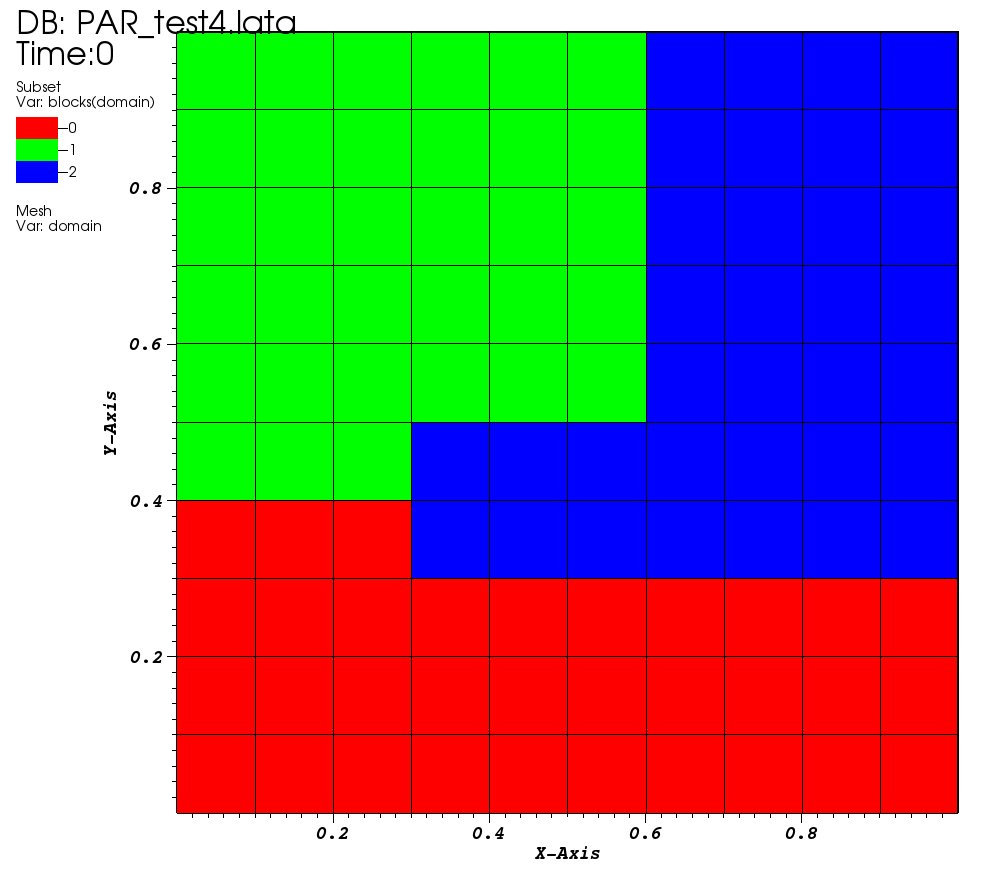
\includegraphics[width=0.45\textwidth]{partition_metis.jpeg} & & 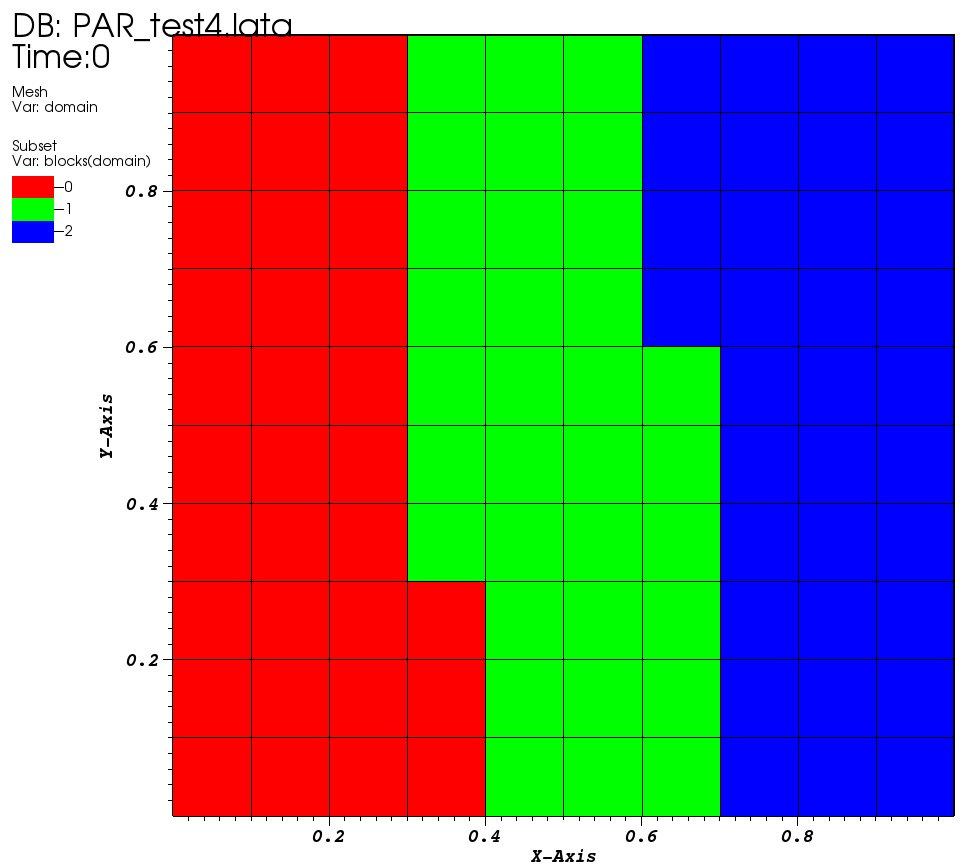
\includegraphics[width=0.45\textwidth]{partition_tranche.jpeg}\tabularnewline
METIS & & Tranche\tabularnewline
\end{tabular}
\par\end{centering}
\caption{Partitioning tools}
\label{partitioning}
\end{figure}

You can see the documentation of \href{\REFERENCEMANUAL\#partition}{this part in the \trustref Reference Manual}.



%%%%%%%%%%%%%%%%%%%%%%%%%%%%%%%%%%%%%%%%%%%%%%%%%
\subsection{Overlapping width value}
%%%%%%%%%%%%%%%%%%%%%%%%%%%%%%%%%%%%%%%%%%%%%%%%%
To make the partitioning, you will have to specify the \underline{overlapping width value}.
This value corresponds to the thickness of the virtual ghost zone (data known by one processor though not owned by it) i.e. the number of vertices or elements on the remote sub-domain known by the local sub-domain (cf Figure \ref{overlap}).

\begin{figure}[h!]
\begin{center}
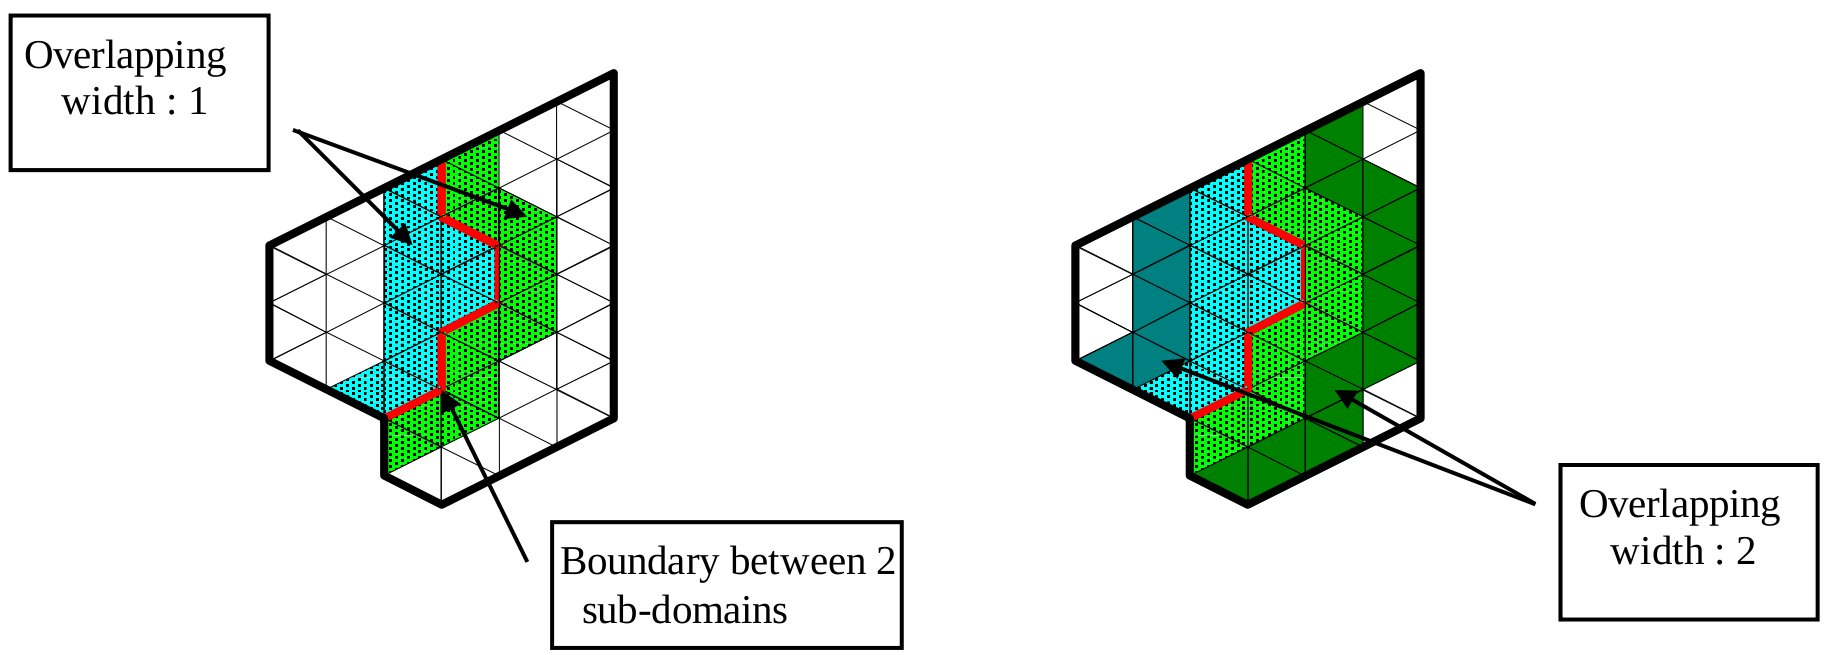
\includegraphics[width=0.96\textwidth]{overlap.jpeg}
\caption{Overlapping width}
\label{overlap}
\end{center}
\end{figure}

This value depends on the space discretization scheme orders:
\begin{itemize}
\item 1 if 1st or 2nd order,
\item 2 if 3rd or 4th order.
\end{itemize}

\Note that in general, you will use "2"!



%%%%%%%%%%%%%%%%%%%%%%%%%%%%%%%%%%%%%%%%%%%%%%%%%%%%%%%%%%%%%%%%%%%%%%%%
\section{Running a parallel calculation}
%%%%%%%%%%%%%%%%%%%%%%%%%%%%%%%%%%%%%%%%%%%%%%%%%%%%%%%%%%%%%%%%%%%%%%%%

%%%%%%%%%%%%%%%%%%%%%%%%%%%%%%%%%%%%%%%%%%%%%%%%%
\subsection{On a PC}
%%%%%%%%%%%%%%%%%%%%%%%%%%%%%%%%%%%%%%%%%%%%%%%%%
To launch the calculation, you have to run the calculation by the usual command completed by the number of processors needed:
\begin{verbatim}
> trust my_parallel_data_file procs_number
\end{verbatim}
and \textit{procs\_number} is the number of processors used. In fact it is the same as the number of sub-domains.\\

You can see the \trust \& \textbf{TrioCFD} user slides in the "Parallel calculation" section for more information and those two exercises of the \trust tutorial: \href{TRUST_tutorial.pdf\#exo_para_1}{exercise 1} and \href{TRUST_tutorial.pdf\#prm_para}{exercise 2}.

%%%%%%%%%%%%%%%%%%%%%%%%%%%%%%%%%%%%%%%%%%%%%%%%%
\subsection{On a cluster}
%%%%%%%%%%%%%%%%%%%%%%%%%%%%%%%%%%%%%%%%%%%%%%%%%
You must submit your job in a queue system.
For this, you must have a submission file.
\trust can create a submission file for you \textbf{on clusters on which the support team has done installations}.
To create this file, run:
\begin{verbatim}
> trust -create_sub_file my_parallel_data_file
\end{verbatim}

You obtain a file named \textbf{"sub\_file"}, you can open it and verify/change values(for example the name of the job, the name of the exe, ...).\\

Then you must submit you calculation with:
\begin{verbatim}
> sbatch sub_file
\end{verbatim}
or 
\begin{verbatim}
> ccc_msub sub_file
\end{verbatim}
following the queue system of the cluster.\\

%You can also run the same command as on a pc:
%\begin{verbatim}
%> trust my_parallel_data_file procs_number
%\end{verbatim}
%\trust will automatically submit your simulation.\\

You can see the \trust \& \textbf{TrioCFD} user slides in the "Parallel calculation" section for more information and \href{TRUST_tutorial.pdf\#exo_para_3}{this exercise of the \trust tutorial}.


%%%%%%%%%%%%%%%%%%%%%%%%%%%%%%%%%%%%%%%%%%%%%%%%%%%%%%%%%%%%%%%%%%%%%%%%
\section{Visualization}
%%%%%%%%%%%%%%%%%%%%%%%%%%%%%%%%%%%%%%%%%%%%%%%%%%%%%%%%%%%%%%%%%%%%%%%%
To visualize your probes, you can use the CurvePlot tool, with the command line:
\begin{verbatim}
> trust -evol my_parallel_data_file
\end{verbatim}
or use Gnuplot or any software which reads values in columns in a file.\\

There are three ways to visualize your parallel results with VisIt:
\begin{itemize}
\item HPCDrive on CCRT/TGCC clusters: opens a deported graphic session on dedicated nodes with more memory (on TGCC cluster: \href{https://visu-tgcc.ccc.cea.fr/HPCDrive/home}{HPCDrive}),
\item local mode: copy your results from the cluster to your local computer and open it with a local parallel version of VisIt with:
\begin{verbatim}
> visit -np 4 &
\end{verbatim}
\end{itemize}

You can have a look at the \trust \& \textbf{TrioCFD} user slides in the "Parallel calculation description" section.




%%%%%%%%%%%%%%%%%%%%%%%%%%%%%%%%%%%%%%%%%%%%%%%%%%%%%%%%%%%%%%%%%%%%%%%%
\section{Useful information}
%%%%%%%%%%%%%%%%%%%%%%%%%%%%%%%%%%%%%%%%%%%%%%%%%%%%%%%%%%%%%%%%%%%%%%%%
%%%%%%%%%%%%%%%%%%%%%%%%%%%%%%%%%%%%%%%%%%%%%%%%%
\subsection{Modify the mesh}
%%%%%%%%%%%%%%%%%%%%%%%%%%%%%%%%%%%%%%%%%%%%%%%%%
If you want to modify your mesh, you have two possibilities:
\begin{itemize} 
\item modify the \textit{my\_data\_file.data} file and run:
\begin{verbatim}
> trust -partition my_data_file [parts_number]
\end{verbatim}
Be carefull it will erase the \textit{SEQ\_my\_data\_file.data}, \textit{DEC\_my\_data\_file.data} and \\
\textit{PAR\_my\_data\_file.data} files and creates new ones.\\
Then it will run the new \textit{DEC\_my\_data\_file.data} file which gives your new \textit{DOM\_000n}\textbf{.Zones} files.

\item modify the meshing part of file \textit{DEC\_my\_data\_file.data} and run it with:
\begin{verbatim}
> trust DEC_my_data_file
\end{verbatim}
\end{itemize}

Then run the parallel calculation normally, on the new \textit{DOM\_000n}\textbf{.Zones} files.
\begin{verbatim}
> trust PAR_my_data_file procs_number
\end{verbatim}




%%%%%%%%%%%%%%%%%%%%%%%%%%%%%%%%%%%%%%%%%%%%%%%%%
\subsection{Modify calculation parameters}
%%%%%%%%%%%%%%%%%%%%%%%%%%%%%%%%%%%%%%%%%%%%%%%%%
If you want to modify the calculation parameters, you can modify:
\begin{itemize} 
\item the file \textit{my\_data\_file.data} and run:
\begin{verbatim}
> trust -partition data_file_name [parts_number]
\end{verbatim}
But it will erase the \textit{SEQ\_my\_data\_file.data}, \textit{DEC\_my\_data\_file.data} and \\
\textit{PAR\_my\_data\_file.data} files and create new ones.\\
Then it will run the new \textit{DEC\_my\_data\_file.data} file which gives your new \textit{DOM\_000n}\textbf{.Zones} files.\\
\Note that in that case, you don't need to re-create the mesh so you can use the second point below:
\item modify the \textit{PAR\_my\_data\_file.data} file \underline{without} running "trust -partition datafile" command line.
\end{itemize}
Then run the \textit{PAR\_my\_data\_file.data} file with:
\begin{verbatim}
> trust PAR_my_data_file procs_number
\end{verbatim}

\Note that if after a certain time, you want to reopen an old case and understand want you did in it without any doubts, you may create two files by hands:
\begin{itemize} 
\item one "BuildMeshes.data" file only for the mesh and the cut of the mesh, and
\item one "calculation.data" file for the parallel calculation. 
\end{itemize}
You will run it like:
\begin{verbatim}
> trust BuildMeshes
> trust calculation processors_number
\end{verbatim}

For this point, you can have a look at \href{TRUST_tutorial.pdf\#prm_para}{this exercise of the \trust tutorial}.






%%%%%%%%%%%%%%%%%%%%%%%%%%%%%%%%%%%%%%%%%%%%%%%%%%%%%%%%%%%%%%%%%%%%%%%%



%%%%%%%%%%%%%%%%%%%%%%%%%%%%%%%%%%%%%%%%%%%%%%%%%%%%%%%%%%%%%%%%%%%%%%%%%%
%%%
%%\chapter{Automatic validation form}
%%%
%%%%%%%%%%%%%%%%%%%%%%%%%%%%%%%%%%%%%%%%%%%%%%%%%%%%%%%%%%%%%%%%%%%%%%%%%%
%%%\input{chap8_prm.tex}
%%%%%%%%%%%%%%%%%%%%%%%%%%%%%%%%%%%%%%%%%%%%%%%%%%%%%%%%%%%%%%%%%%%%%%%%%%



\end{document}

'

\usepackage[unicode=true,pdfusetitle, bookmarks=true,bookmarksnumbered=false,bookmarksopen=false,
 breaklinks=false,pdfborder={0 0 1},backref=false,colorlinks=true,linkcolor=blue,pageanchor, urlcolor=darkblue]
 {hyperref}[2010/09/11]

\ifx \TRUSTV \undefined
\def\TRUSTVERSION{}
\else
\def\TRUSTVERSION{V\TRUSTV}
\fi
%\def \REFERENCEMANUAL {../../Outils/TRIOXDATA/XTriou/doc.pdf}
\def \REFERENCEMANUAL {TRUST_Reference_Manual.pdf}

\hypersetup{pdftitle={TRUST Generic Guide \TRUSTVERSION}, pdfauthor={Team TRUST} }

\usepackage[utf8]{inputenc}
\usepackage[T1]{fontenc}
\usepackage[top=2cm, bottom=2cm, left=2cm, right=2cm]{geometry}
\usepackage{babel}
\usepackage{alltt}
\usepackage{color}
\usepackage{longtable}
\usepackage{tikz}
\usepackage{xspace}
\usepackage{graphicx}
%\usepackage{times}

\setlength{\parindent}{0pt} % pas d'indentation

\definecolor{darkblue}{HTML}{3535B4}
\definecolor{LightSkyBlue}{HTML}{87CFFA}
\definecolor{DeepSkyBlue}{HTML}{00BFFF}
\definecolor{Greeen}{HTML}{439236}
\definecolor{mauve}{HTML}{874ad3}
\definecolor{vert}{HTML}{0ab351}
\definecolor{darkred}{HTML}{a31623}

\newenvironment{remark}{\textit{\underline{Remark:}}}{}
\newcommand{\trust}{\textbf{TRUST}\xspace}
\newcommand{\trustref}{Project\xspace}
\newcommand{\Note}{\textbf{\textcolor{darkred}{Note}}\xspace}


\begin{document}

\title{\vspace{2cm}\Huge \bfseries{TRUST Generic Guide \TRUSTVERSION}}
\author{
\vspace{2cm} % espace entre support team et ref manual
\LARGE \textbf{Support team: \href{mailto:triou@cea.fr}{triou@cea.fr}} \\
\vspace{1cm} % espace entre ref manual et la date
Link to: \LARGE \textbf{\href{run:\REFERENCEMANUAL}{\trustref Reference Manual}}\\
%%%%%%% Pour recuperer l'adresse d'un pdf par les variables d'environnement et makefile
%%%%%\ifx \BALTROOT \empty
%%%%%Link to: \LARGE \textbf{\href{run:\TRUSTROOTLATEX/Outils/TRIOXDATA/XTriou/doc.pdf}{\trustref Reference Manual}}\\
%%%%%\else
%%%%%Link to: \LARGE \textbf{\href{run:\BALTROOT/build/xdata/XTriou/doc.pdf}{\trustref Reference Manual}}\\
%%%%%\fi
}
%\date{} % si on ne veut pas la date

\maketitle
\tableofcontents{}
\newpage


%%%%%%%%%%%%%%%%%%%%%%%%%%%%%%%%%%%%%%%%%%%%%%%%%%%%%%%%%%%%%%%%%%%%%%%%
%
\chapter{Introduction}
%
%%%%%%%%%%%%%%%%%%%%%%%%%%%%%%%%%%%%%%%%%%%%%%%%%%%%%%%%%%%%%%%%%%%%%%%%
This document constitutes the generic guide for \textbf{TRUST software} and its \textbf{Baltik projects}.\\

\trust is a thermohydraulic software package for CFD simulations for incompressible monophasic flow.\\

You can create new project based on \trust plateform. Theses projects are named \textbf{"BALTIK"} projects.\\

The currently available modules include a VDF calculation module "Finite Difference Volume", a VEF calculation module "Finite Element Volume" and a PolyMAC module "series of Marker-and-Cell (MAC) schemes that can handle any type of mesh (non-conform, non-orthogonal, poly-hedral types, ...)". For further details, you can see https://cea-trust-platform.github.io/classes/discretizations/ \\

The VDF and VEF validated modules are designed to process the 2D or 3D flow of Newtonian, incompressible, weakly expandable fluids the density of which is a function of a local temperature and concentration values (Boussinesq approximation).



%%%%%%%%%%%%%%%%%%%%%%%%%%%%%%%%%%%%%%%%%%%%%%%%%%%%%%%%%%%%%%%
\section{Before TRUST: a modular software named Trio\_U}
%%%%%%%%%%%%%%%%%%%%%%%%%%%%%%%%%%%%%%%%%%%%%%%%%%%%%%%%%%%%%%%

\trust was born from the cutting in two pieces of \textbf{Trio\_U} software.
\textbf{Trio\_U} was a software brick based on the \textbf{Kernel} brick (which contains the equations, space discretizations, numerical schemes, parallelism...) and used by other CEA applications (cf Figure \ref{TrioU}).

\begin{figure}[h!]
\begin{center}
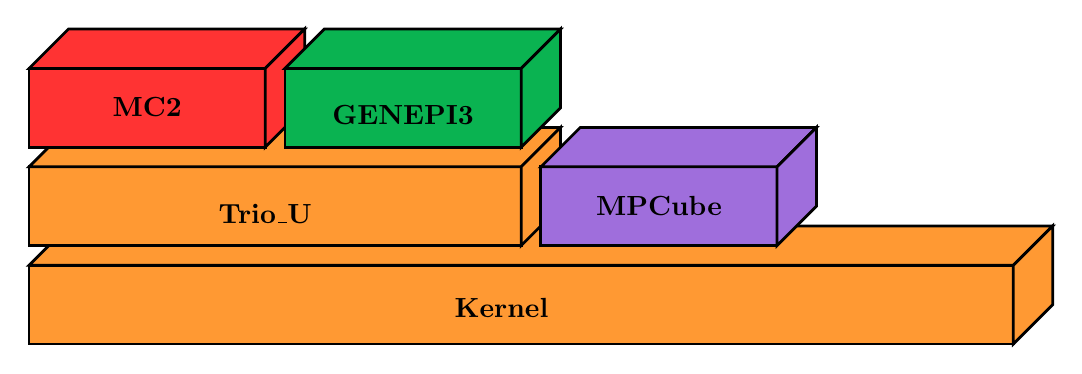
\begin{tikzpicture}[scale=2, line width=1pt]
% box Kernel
\coordinate (A) at (0,0) ;
\coordinate (B) at (6.25,0) ;
\coordinate (C) at (6.25,0.5) ;
\coordinate (D) at (0,0.5) ;
\coordinate (E) at (0.25,0.75) ;
\coordinate (F) at (6.5,0.75) ;
\coordinate (G) at (6.5,0.25) ;
\draw[black,fill=orange!80] (A) -- (B) -- (C) -- (D) -- cycle ;
\draw[black,fill=orange!80] (D) -- (C) -- (F) -- (E) -- cycle ;
\draw[black,fill=orange!80] (B) -- (C) -- (F) -- (G) -- cycle ;
\draw (3,0.1) node[above]{\textbf{Kernel}} ;
%% box Trio_U
\begin{scope}
\coordinate (A1) at (0,0.625) ;
\coordinate (B1) at (3.125,0.625) ;
\coordinate (C1) at (3.125,1.125) ;
\coordinate (D1) at (0,1.125) ;
\coordinate (E1) at (0.25,1.375) ;
\coordinate (F1) at (3.375,1.375) ;
\coordinate (G1) at (3.375,0.875) ;
\draw[black,fill=orange!80] (A1) -- (B1) -- (C1) -- (D1) -- cycle ;
\draw[black,fill=orange!80] (D1) -- (C1) -- (F1) -- (E1) -- cycle ;
\draw[black,fill=orange!80] (B1) -- (C1) -- (F1) -- (G1) -- cycle ;
\draw (1.5,0.7) node[above]{\textbf{Trio\_U}} ;
\end{scope}
% box MPCube
\begin{scope}[xshift=3.25 cm]
\coordinate (A1) at (0,0.625) ;
\coordinate (B1) at (1.5,0.625) ;
\coordinate (C1) at (1.5,1.125) ;
\coordinate (D1) at (0,1.125) ;
\coordinate (E1) at (0.25,1.375) ;
\coordinate (F1) at (1.75,1.375) ;
\coordinate (G1) at (1.75,0.875) ;
\draw[black,fill=mauve!80] (A1) -- (B1) -- (C1) -- (D1) -- cycle ;
\draw[black,fill=mauve!80] (D1) -- (C1) -- (F1) -- (E1) -- cycle ;
\draw[black,fill=mauve!80] (B1) -- (C1) -- (F1) -- (G1) -- cycle ;
\draw (0.75,0.75) node[above]{\textbf{MPCube}} ;
\end{scope}
%% box MC2
\begin{scope}[xshift=0 cm, yshift=0.625 cm]
\coordinate (A1) at (0,0.625) ;
\coordinate (B1) at (1.5,0.625) ;
\coordinate (C1) at (1.5,1.125) ;
\coordinate (D1) at (0,1.125) ;
\coordinate (E1) at (0.25,1.375) ;
\coordinate (F1) at (1.75,1.375) ;
\coordinate (G1) at (1.75,0.875) ;
\draw[black,fill=red!80] (A1) -- (B1) -- (C1) -- (D1) -- cycle ;
\draw[black,fill=red!80] (D1) -- (C1) -- (F1) -- (E1) -- cycle ;
\draw[black,fill=red!80] (B1) -- (C1) -- (F1) -- (G1) -- cycle ;
\draw (0.75,0.75) node[above]{\textbf{MC2}} ;
\end{scope}
% box GENEPI3
\begin{scope}[xshift=1.625 cm, yshift=0.625 cm]
\coordinate (A1) at (0,0.625) ;
\coordinate (B1) at (1.5,0.625) ;
\coordinate (C1) at (1.5,1.125) ;
\coordinate (D1) at (0,1.125) ;
\coordinate (E1) at (0.25,1.375) ;
\coordinate (F1) at (1.75,1.375) ;
\coordinate (G1) at (1.75,0.875) ;
\draw[black,fill=vert] (A1) -- (B1) -- (C1) -- (D1) -- cycle ;
\draw[black,fill=vert] (D1) -- (C1) -- (F1) -- (E1) -- cycle ;
\draw[black,fill=vert] (B1) -- (C1) -- (F1) -- (G1) -- cycle ;
\draw (0.75,0.7) node[above]{\textbf{GENEPI3}} ;
\end{scope}
\end{tikzpicture}
\caption{Trio\_U: brick software}
\label{TrioU}
\end{center}
\end{figure}

We could create new projects based on Kernel brick or \textbf{Trio\_U} brick. 
Theses projects were named \textbf{"BALTIK"} projects: "\textbf{B}uild an \textbf{A}pplication \textbf{L}inked to \textbf{T}r\textbf{I}o\_U \textbf{K}ernel".\\

In 2015, \textbf{Trio\_U} was divided in two parts: \trust and \textbf{TrioCFD}.
\begin{itemize}
\item \trust is a new platform, its name means: "\textbf{TR}io\_\textbf{U} \textbf{S}oftware for \textbf{T}hermohydraulics",
\item \textbf{TrioCFD} is a BALTIK project based on \trust, which contains the following models: FT, Radiation, LES, zoom...
\end{itemize}

Here is the structure of \trust platform (cf Figure \ref{TRUST}):

\begin{figure}[h!]
\begin{center}
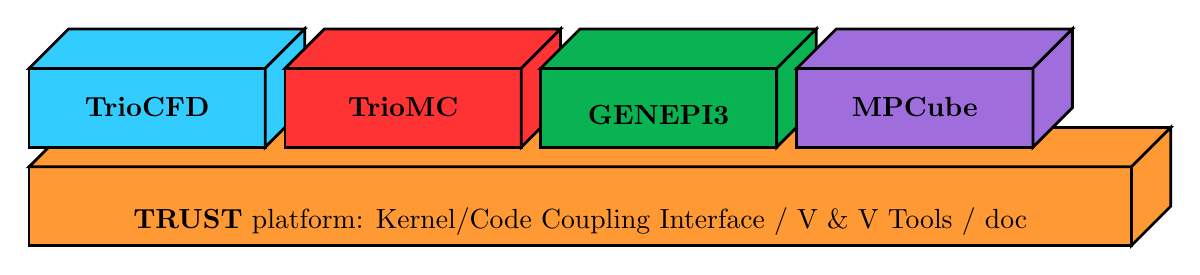
\begin{tikzpicture}[scale=2, line width=1pt]
% box TRUST
\coordinate (A) at (0,0) ;
\coordinate (B) at (7,0) ;
\coordinate (C) at (7,0.5) ;
\coordinate (D) at (0,0.5) ;
\coordinate (E) at (0.25,0.75) ;
\coordinate (F) at (7.25,0.75) ;
\coordinate (G) at (7.25,0.25) ;
\draw[black,fill=orange!80] (A) -- (B) -- (C) -- (D) -- cycle ;
\draw[black,fill=orange!80] (D) -- (C) -- (F) -- (E) -- cycle ;
\draw[black,fill=orange!80] (B) -- (C) -- (F) -- (G) -- cycle ;
\draw (3.5,0) node[above]{\trust platform: Kernel/Code Coupling Interface / V \& V Tools / doc} ;
%% box TrioCFD
\begin{scope}
\coordinate (A1) at (0,0.625) ;
\coordinate (B1) at (1.5,0.625) ;
\coordinate (C1) at (1.5,1.125) ;
\coordinate (D1) at (0,1.125) ;
\coordinate (E1) at (0.25,1.375) ;
\coordinate (F1) at (1.75,1.375) ;
\coordinate (G1) at (1.75,0.875) ;
\draw[black,fill=DeepSkyBlue!80] (A1) -- (B1) -- (C1) -- (D1) -- cycle ;
\draw[black,fill=DeepSkyBlue!80] (D1) -- (C1) -- (F1) -- (E1) -- cycle ;
\draw[black,fill=DeepSkyBlue!80] (B1) -- (C1) -- (F1) -- (G1) -- cycle ;
\draw (0.75,0.75) node[above]{\textbf{TrioCFD}} ;
\end{scope}
% box TrioMC
\begin{scope}[xshift=1.625 cm]
\coordinate (A1) at (0,0.625) ;
\coordinate (B1) at (1.5,0.625) ;
\coordinate (C1) at (1.5,1.125) ;
\coordinate (D1) at (0,1.125) ;
\coordinate (E1) at (0.25,1.375) ;
\coordinate (F1) at (1.75,1.375) ;
\coordinate (G1) at (1.75,0.875) ;
\draw[black,fill=red!80] (A1) -- (B1) -- (C1) -- (D1) -- cycle ;
\draw[black,fill=red!80] (D1) -- (C1) -- (F1) -- (E1) -- cycle ;
\draw[black,fill=red!80] (B1) -- (C1) -- (F1) -- (G1) -- cycle ;
\draw (0.75,0.75) node[above]{\textbf{TrioMC}} ;
\end{scope}
% box GENEPI3
\begin{scope}[xshift=3.248 cm]
\coordinate (A1) at (0,0.625) ;
\coordinate (B1) at (1.5,0.625) ;
\coordinate (C1) at (1.5,1.125) ;
\coordinate (D1) at (0,1.125) ;
\coordinate (E1) at (0.25,1.375) ;
\coordinate (F1) at (1.75,1.375) ;
\coordinate (G1) at (1.75,0.875) ;
\draw[black,fill=vert] (A1) -- (B1) -- (C1) -- (D1) -- cycle ;
\draw[black,fill=vert] (D1) -- (C1) -- (F1) -- (E1) -- cycle ;
\draw[black,fill=vert] (B1) -- (C1) -- (F1) -- (G1) -- cycle ;
\draw (0.75,0.7) node[above]{\textbf{GENEPI3}} ;
\end{scope}
%% box MPCube
\begin{scope}[xshift=4.875 cm]
\coordinate (A1) at (0,0.625) ;
\coordinate (B1) at (1.5,0.625) ;
\coordinate (C1) at (1.5,1.125) ;
\coordinate (D1) at (0,1.125) ;
\coordinate (E1) at (0.25,1.375) ;
\coordinate (F1) at (1.75,1.375) ;
\coordinate (G1) at (1.75,0.875) ;
\draw[black,fill=mauve!80] (A1) -- (B1) -- (C1) -- (D1) -- cycle ;
\draw[black,fill=mauve!80] (D1) -- (C1) -- (F1) -- (E1) -- cycle ;
\draw[black,fill=mauve!80] (B1) -- (C1) -- (F1) -- (G1) -- cycle ;
\draw (0.75,0.75) node[above]{\textbf{MPCube}} ;
\end{scope}
\end{tikzpicture}
\caption{TRUST platform \& its BALTIKs}
\label{TRUST}
\end{center}
\end{figure}

\Note that: \textbf{Trio\_U = TRUST + TrioCFD}.
%%%%%%%%%%%%%%%%%%%%%%%%%%%%%%%%%%%%%%%%%%%%%%%%%%%%%%%%%%%%%%%



%%%%%%%%%%%%%%%%%%%%%%%%%%%%%%%%%%%%%%%%%%%%%%%%%%%%%%%%%%%%%%%
\section{Short history}
%%%%%%%%%%%%%%%%%%%%%%%%%%%%%%%%%%%%%%%%%%%%%%%%%%%%%%%%%%%%%%%

\trust is now developed at the CEA/DES/ISAS/DM2S/SGLS service.
The project starts in 1994 and improved versions were built ever since:
\begin{itemize}
\item 1994: start of the project Trio\_U
\item 01/1997: v1.0 - VDF only
\item 06/1998: v1.1 - VEF version
\item 04/2000: v1.2 - parallel version
\item 07/2001: v1.3 - radiation model, in TrioCFD since v1.7
\item 11/2002: v1.4 - new LES turbulence models, in TrioCFD since v1.8
\item 02/2006: v1.5 - VDF/VEF Front Tracking, in TrioCFD since v1.7
\item 10/2009: v1.6 - data structure revamped
\item 06/2015: v1.7 - cut into \trust and \textbf{TrioCFD} + switch to open source
\item 11/2019: v1.8 - Turbulence features are moved from \trust to \textbf{TrioCFD} + PolyMAC discretization
\item 06/2022: v1.9 - Pb\_Multiphase in \trust + PolyMAC V2 discretization + Pb\_HEM in \textbf{TrioCFD}
\end{itemize}
%%%%%%%%%%%%%%%%%%%%%%%%%%%%%%%%%%%%%%%%%%%%%%%%%%%%%%%%%%%%%%%




%%%%%%%%%%%%%%%%%%%%%%%%%%%%%%%%%%%%%%%%%%%%%%%%%%%%%%%%%%%%%%%
\section{Data file}
%%%%%%%%%%%%%%%%%%%%%%%%%%%%%%%%%%%%%%%%%%%%%%%%%%%%%%%%%%%%%%%

To launch a calculation with \trust, you need to write a "data file" which is an input file for \trust and will contain all the information about your simulation.
Data files are written following some rules as shown below. But their language is not a programming language, users can't make loops or switch...\\

\Note that:
\begin{itemize}
\item lines between \textcolor{blue}{\# ... \#} and \textcolor{blue}{/* ... */} are comments,
\item in that document, words in \textbf{bold} are \trust keywords, you can highlight them in your file editor with the command line (details in section \ref{Run}):\\
\texttt{> trust -config gedit|vim|emacs}
\item braces "\{ \}" are elements that \trust reads and interprets, so don't forget them and \underline{put space} \underline{before and after them},
\item elements between bracket "[ ]" are optional.
\end{itemize}

%%%%%%%%%%%%%%%%%%%%%%%%%%%%%%%%%%%%%%%%%%%%%%%%%%%%
\subsection{Data file example: base blocks} \label{data}
%%%%%%%%%%%%%%%%%%%%%%%%%%%%%%%%%%%%%%%%%%%%%%%%%%%%
Here is the template of a basic sequential data file:\\

\fbox{ \begin{minipage}[c]{1\textwidth}
\begin{alltt}
\textcolor{blue}{\# Dimension 2D or 3D \#}

{\bf{Dimension}} 2
\end{alltt}
\end{minipage}}
\vspace{0.1cm}



\fbox{ \begin{minipage}[c]{1\textwidth}
\begin{alltt}
\textcolor{blue}{\# Problem definition \#}

{\bf{Pb\_hydraulique}} \textit{my\_problem}
\end{alltt}
\end{minipage}}
\vspace{0.1cm}



\fbox{ \begin{minipage}[c]{1\textwidth}
\begin{alltt}
\textcolor{blue}{\# Domain definition \#}

{\bf{Domaine}} \textit{my\_domain}
\end{alltt}
\end{minipage}}
\vspace{0.1cm}



\fbox{ \begin{minipage}[c]{1\textwidth}
\begin{alltt}
\textcolor{blue}{\# Mesh \#}

{\bf{Read\_file}} \textit{my\_mesh.geo} ;
\end{alltt}
\end{minipage}}
\vspace{0.1cm}



\fbox{ \begin{minipage}[c]{1\textwidth}
\begin{alltt} 
\textcolor{blue}{\# For parallel calculation only! \#}

\textcolor{blue}{\# For the first run: partitioning step \#}

\textcolor{blue}{{\bf{Partition}} \textit{my\_domain}}

\textcolor{blue}{\{}

\textcolor{blue}{\hspace{1cm}    {\bf{Partition\_tool}} \textit{partitioner\_name} \{ \textit{option1 option2 ...} \}}

\textcolor{blue}{\hspace{1cm}    {\bf{Larg\_joint}} \textit{2}}

\textcolor{blue}{\hspace{1cm}    {\bf{zones\_name}} \textit{DOM}}

\textcolor{blue}{\hspace{1cm}    ...}

\textcolor{blue}{\}}

\textcolor{blue}{{\bf{End}}}
\end{alltt}
\end{minipage}}
\vspace{0.1cm}



\fbox{ \begin{minipage}[c]{1\textwidth}
\begin{alltt} 
\textcolor{blue}{\# For parallel calculation only! \#}

\textcolor{blue}{\# For the second run: read of the sub-domains \#}

\textcolor{blue}{\# {\bf{Scatter}} \textit{DOM}{\bf{.Zones}} \textit{my\_domain} \#}
\end{alltt}
\end{minipage}}
\vspace{0.1cm}



\fbox{ \begin{minipage}[c]{1\textwidth}
\begin{alltt}
\textcolor{blue}{\# Discretization on hexa or tetra mesh \#}

{\bf{VDF}} \textit{my\_discretization}
\end{alltt}
\end{minipage}}
\vspace{0.1cm}



\fbox{ \begin{minipage}[c]{1\textwidth}
\begin{alltt}
\textcolor{blue}{\# Time scheme explicit or implicit \#}

{\bf{Scheme\_euler\_explicit}} \textit{my\_scheme}

{\bf{Read}} \textit{my\_scheme}

\{

\hspace{1cm}        \textcolor{blue}{\# Initial time \#}

\hspace{1cm}        \textcolor{blue}{\# Time step \#}

\hspace{1cm}        \textcolor{blue}{\# Output criteria \#}

\hspace{1cm}        \textcolor{blue}{\# Stop Criteria \#}

\}
\end{alltt}
\end{minipage}}
\vspace{0.1cm}



\fbox{ \begin{minipage}[c]{1\textwidth}
\begin{alltt}
\textcolor{blue}{\# Physical characteristics of medium \#}

{\bf{Fluide\_Incompressible}} \textit{my\_medium}

{\bf{Read}} \textit{my\_medium}

\{

\hspace{1cm}        ...

\}
\end{alltt}
\end{minipage}}
\vspace{0.1cm}



\fbox{ \begin{minipage}[c]{1\textwidth}
\begin{alltt}
\textcolor{blue}{\# Gravity vector definition \#}

{\bf{Uniform\_field}} \textit{my\_gravity}

{\bf{Read}} \textit{my\_gravity 2 0 -9.81}

\end{alltt}
\end{minipage}}
\vspace{0.1cm}



\fbox{ \begin{minipage}[c]{1\textwidth}
\begin{alltt}

\textcolor{blue}{\# Association between the different objects \#}

{\bf{Associate}} \textit{my\_problem my\_domain}

{\bf{Associate}} \textit{my\_problem my\_scheme}

{\bf{Associate}} \textit{my\_problem my\_medium}

{\bf{Associate}} \textit{my\_medium my\_gravity}
\end{alltt}
\end{minipage}}
\vspace{0.1cm}



\fbox{ \begin{minipage}[c]{1\textwidth}
\begin{alltt}
\textcolor{blue}{\# Discretization of the problem \#}

{\bf{Discretize}} \textit{my\_problem my\_discretization}
\end{alltt}
\end{minipage}}
\vspace{0.1cm}



\fbox{ \begin{minipage}[c]{1\textwidth}
\begin{alltt}
\textcolor{blue}{\# New domains for post-treatment \#}

\textcolor{blue}{\# By default each boundary condition of the domain is already extrated }

\textcolor{blue}{\hspace{0.2cm} with such name "my\_dom"\_boundaries\_"my\_BC" \#}

{\bf{Domaine}} \textit{plane}

{\bf{extraire\_surface}} 

\{

\hspace{1cm}        {\bf{domaine}} \textit{plane}

\hspace{1cm}        {\bf{probleme}} \textit{my\_probleme}

\hspace{1cm}        {\bf{condition\_elements}} (x>0.5)

\hspace{1cm}        {\bf{condition\_faces (1)}} 

\}
\end{alltt}
\end{minipage}}
\vspace{0.1cm}



\fbox{ \begin{minipage}[c]{1\textwidth}
\begin{alltt}
\textcolor{blue}{\# Problem description \#}

{\bf{Read}} \textit{my\_problem}

\{
\end{alltt}
\end{minipage}}
\vspace{0.1cm}



\fbox{ \begin{minipage}[c]{1\textwidth}
\begin{alltt}
\hspace{1cm}        \textcolor{blue}{\# hydraulic problem \#}

\hspace{1cm}        {\bf{Navier\_Stokes\_standard}}

\hspace{1cm}        \{

\hspace{2cm}                \textcolor{blue}{\# Choice of the pressure matrix solver \#}

\hspace{2cm}                {\bf{Solveur\_Pression}} \textit{solver} \{ ... \}

\hspace{2cm}                \textcolor{blue}{\# Diffusion operator \#}

\hspace{2cm}                {\bf{Diffusion}} \{ ... \}

\hspace{2cm}                \textcolor{blue}{\# Convection operator \#}

\hspace{2cm}                {\bf{Convection}} \{ ... \}

\hspace{2cm}                \textcolor{blue}{\# Sources \#}

\hspace{2cm}                {\bf{Sources}} \{ ... \}

\hspace{2cm}                \textcolor{blue}{\# Initial conditions \#}

\hspace{2cm}                {\bf{Initial\_conditions}} \{ ... \}

\hspace{2cm}                \textcolor{blue}{\# Boundary conditions \#}

\hspace{2cm}                {\bf{Boundary\_conditions}} \{ ... \}

\hspace{1cm}        \}
    \end{alltt}
\end{minipage}}
\vspace{0.1cm}



\fbox{ \begin{minipage}[c]{1\textwidth}
\begin{alltt}
\hspace{1cm}        \textcolor{blue}{\# Post\_processing description \#}

\hspace{1cm}        \textcolor{blue}{/* To know domains that can be treated directly, search in .err }

\hspace{1.6cm}       \textcolor{blue}{    output file: "Creating a surface domain named" */}

\hspace{1cm}        \textcolor{blue}{/* To know fields  that can be treated directly, search in .err }

\hspace{1.6cm}      \textcolor{blue}{     output file: "Reading of fields to be postprocessed" */}

\hspace{1cm}        {\bf{Post\_processing}}

\hspace{1cm}        \{

\hspace{2cm}                \textcolor{blue}{\# Definition of new fields \#}

\hspace{2cm}                {\bf{Definition\_Champs}} \{ ... \}


\hspace{2cm}                \textcolor{blue}{\# Probes \#}

\hspace{2cm}                {\bf{Probes}} \{ ... \}


\hspace{2cm}                \textcolor{blue}{\# Fields \#}

\hspace{2cm}                \textcolor{blue}{\# format default value: lml \#}

\hspace{2cm}                \textcolor{blue}{\# select 'lata' for VisIt tool or 'MED' for Salom\'e \#}

\hspace{2cm}                {\bf{format lata}}

\hspace{2cm}                {\bf{fields dt\_post}} 1. \{ ... \}


\hspace{2cm}                \textcolor{blue}{\# Statistical fields \#}

\hspace{2cm}                {\bf{Statistiques dt\_post}} 1. \{ ... \}

\hspace{1cm}        \} 
\end{alltt}
\end{minipage}}
\vspace{0.1cm}



\fbox{ \begin{minipage}[c]{1\textwidth}
\begin{alltt}
    \textcolor{blue}{\# Saving and restarting process \#}

    [{\bf{sauvegarde binaire}} \textit{datafile}{\bf{.sauv}}]

    [{\bf{resume\_last\_time binaire}} \textit{datafile}{\bf{.sauv}}]
\end{alltt}
\end{minipage}}
\vspace{0.1cm}


\fbox{ \begin{minipage}[c]{1\textwidth}
\begin{alltt}
\textcolor{blue}{\# End of the problem description block \#}

\}
\end{alltt}
\end{minipage}}
\vspace{0.1cm}



\fbox{ \begin{minipage}[c]{1\textwidth}
\begin{alltt}
\textcolor{blue}{\# The problem is solved with \#}

{\bf{Solve}} \textit{my\_problem}
\end{alltt}
\end{minipage}}
\vspace{0.1cm}



\fbox{ \begin{minipage}[c]{1\textwidth}
\begin{alltt}
\textcolor{blue}{\# Not necessary keyword to finish \#}

{\bf{End}}
\end{alltt}
\end{minipage}}


%%%%%%%%%%%%%%%%%%%%%%%%%%%%%%%%%%%%%%%%%%%%%%%%%%%%



%%%%%%%%%%%%%%%%%%%%%%%%%%%%%%%%%%%%%%%%%%%%%%%%%%%%
\subsection{Basic rules}
%%%%%%%%%%%%%%%%%%%%%%%%%%%%%%%%%%%%%%%%%%%%%%%%%%%%
There is no line concept in \trust.\\

Data files uses \underline{blocks}. They may be defined using the braces:\\
    \begin{center}
    \fbox{ \begin{minipage}[c]{0.5\textwidth}
    \begin{alltt}
    \{

    \hspace{1cm}    a block

    \}
    \end{alltt}
    \end{minipage}}
    \end{center}
\bigskip{}


%%%%%%%%%%%%%%%%%%%%%%%%%%%%%%%%%%%%%%%%%%%%%%%%%%%%



%%%%%%%%%%%%%%%%%%%%%%%%%%%%%%%%%%%%%%%%%%%%%%%%%%%%
\subsection{Objects notion}
%%%%%%%%%%%%%%%%%%%%%%%%%%%%%%%%%%%%%%%%%%%%%%%%%%%%
\textbf{Objects} are created in the data set as follows:
    \begin{center}
    \fbox{ \begin{minipage}[c]{0.5\textwidth}
    \begin{alltt}
        {\textit{ Type identificateur}}
    \end{alltt}
    \end{minipage}}
    \end{center}

\begin{itemize}
\item \textit{Type}: must be a type of object recognised by \trust, correspond to the C++ classes. The list of recognised types is given in the file hierarchie.dump.
\item \textit{identificateur}: the identifier of the object type \textit{Type} created, correspond to an instancy of the C++ class \textit{Type}. \trust exits in error if the identifier has already been used.
\end{itemize}

There are several object types. Physical objects, for example:

\begin{itemize}
%\item A block object (keyword \textbf{Pave}) is defined by its origin and dimensions (keyword \textbf{origine (origin)} and \textbf{longueurs (length)}). Discretization is given by the \textbf{nombre\_de\_noeuds (node number)} in each direction.
\item A \textbf{Fluide\_incompressible} (incompressible\_Fluid) object. This type of object is defined by its physical characteristics (its dynamic viscosity $\mu$ (keyword \textbf{mu}), its density $\rho$ (keyword \textbf{rho}), etc...),
\item A \textbf{Domaine}.
\end{itemize}

More abstract object types also exist:

\begin{itemize}
\item A \textbf{VDF}, \textbf{VEF} or \textbf{PolyMAC} according to the discretization type,
\item A \textbf{Scheme\_euler\_explicit} to indicate the time scheme type, here it's a first-order explicit Euler scheme,
\item A \textbf{Solveur\_pression} to denote the pressure system solver type,
\item A \textbf{Uniform\_field} to define, for example, the gravity field.
\end{itemize}
%%%%%%%%%%%%%%%%%%%%%%%%%%%%%%%%%%%%%%%%%%%%%%%%%%%%



%%%%%%%%%%%%%%%%%%%%%%%%%%%%%%%%%%%%%%%%%%%%%%%%%%%%
\subsection{Interpretor notion}
%%%%%%%%%%%%%%%%%%%%%%%%%%%%%%%%%%%%%%%%%%%%%%%%%%%%
\textbf{Interprete } (interpretor) type objects are then used to handle the created objects with the following syntax:
    \begin{center}
    \fbox{ \begin{minipage}[c]{0.5\textwidth}
    \begin{alltt}
        {\bf{\textit{Type\_interprete}}} \textit{argument}
    \end{alltt}
    \end{minipage}}
    \end{center}

\begin{itemize}
\item \textit{Type\_interprete}: any type derived from the \textbf{Interprete} (Interpretor) type recognised by \trust. In this manual, they are written in \textbf{bold}. You can highlight them in your file editor with the command (details in section \ref{Run}):\\
\texttt{> trust -config nedit|vim|emacs}
\item \textit{argument}: an argument may comprise one or several object identifiers and/or one or several data blocks.
\end{itemize}

Interpretors allow some operations to be carried out on objects.\\

Currently available general interpretors include \textbf{Read}, \textbf{Read\_file}, \textbf{Ecrire} (Write), \textbf{Ecrire\_fichier} (Write\_file), \textbf{Associate}.
%%%%%%%%%%%%%%%%%%%%%%%%%%%%%%%%%%%%%%%%%%%%%%%%%%%%



%%%%%%%%%%%%%%%%%%%%%%%%%%%%%%%%%%%%%%%%%%%%%%%%%%%%
\subsection{Example}
%%%%%%%%%%%%%%%%%%%%%%%%%%%%%%%%%%%%%%%%%%%%%%%%%%%%
%\begin{itemize}
%\item A data set to write Ok on screen:
A data set to write Ok on screen:
    \begin{center}
    \fbox{ \begin{minipage}[c]{0.9\textwidth}
    \begin{alltt}
    {\bf{Nom}} a\_name    \hspace{0.5cm}       \textcolor{blue}{\# Creation of an object type. Name identifier a\_name \#}

    {\bf{Read}} a\_name Ok        \textcolor{blue}{\# Allocates the string "Ok" to a\_name \#}

    {\bf{Ecrire}} a\_name     \hspace{0.2cm}     \textcolor{blue}{\# Write a\_name on screen \#}
    \end{alltt}
    \end{minipage}}
    \end{center}

%%%\item An incorrect data set:
%%%    \begin{center}
%%%    \fbox{ \begin{minipage}[c]{0.5\textwidth}
%%%    \begin{alltt}
%%%    {\bf{Domaine}} truc

%%%    ...

%%%    {\bf{Probleme}} truc   \textcolor{blue}{\# TRUST exits in error \#}
%%%    \end{alltt}
%%%    \end{minipage}}
%%%    \end{center}

%%%A possible correction:
%%%    \begin{center}
%%%    \fbox{ \begin{minipage}[c]{0.9\textwidth}
%%%    \begin{alltt}
%%%    \{

%%%    {\bf{Domaine}} truc

%%%    \}   \hspace{2.6cm}   \textcolor{blue}{\# The domain truc is destroyed \#}

%%%    {\bf{Probleme}} truc  \textcolor{blue}{\# this is correct because truc is not used any more \#}
%%%    \end{alltt}
%%%    \end{minipage}}
%%%    \end{center}


%\item One data set nesting another:
%    \begin{center}
%    \fbox{ \begin{minipage}[c]{0.9\textwidth}
%    \begin{alltt}
%    {\bf{Read\_file}} fichier\_inclus ; 

%    \textcolor{blue}{\# you should use {\bf{export}} in the fichier\_inclus to export identifiers \#}
%    \end{alltt}
%    \end{minipage}}
%    \end{center}

%example of the fichier\_inclus file: 
%    \begin{center}
%    \fbox{ \begin{minipage}[c]{0.9\textwidth}
%    \begin{alltt}
%    {\bf{Dimension}} 2

%    {\bf{export Domaine}} dom

%    {\bf{export Probleme\_hydraulique}} pb
%    \end{alltt}
%    \end{minipage}}
%    \end{center}
%\end{itemize}
%%%%%%%%%%%%%%%%%%%%%%%%%%%%%%%%%%%%%%%%%%%%%%%%%%%%



%%%%%%%%%%%%%%%%%%%%%%%%%%%%%%%%%%%%%%%%%%%%%%%%%%%%
\subsection{Important remarks}
%%%%%%%%%%%%%%%%%%%%%%%%%%%%%%%%%%%%%%%%%%%%%%%%%%%%
\begin{enumerate}
\item To insert \underline{comments} in the data set, use \textcolor{blue}{\# .. \#} (or \textcolor{blue}{/* ... */}), the character \textcolor{blue}{\#} must always be enclosed by blanks.
\item The comma separates items in a list (a comma must be enclosed with spaces or a new line).
\item Interpretor keywords are recognised indiscriminately whether they are written in lower and/or upper case.
\item \textbf{On the contrary, object names (identifiers) are recognised differently if they are written in upper or lower case.}
\item In the following description, items (keywords or values) enclosed by [ and ] are \underline{optional}.
\end{enumerate}
%%%%%%%%%%%%%%%%%%%%%%%%%%%%%%%%%%%%%%%%%%%%%%%%%%%%



%%%%%%%%%%%%%%%%%%%%%%%%%%%%%%%%%%%%%%%%%%%%%%%%%%%%%%%%%%%%%%%
\section{Running a data file}\label{Run}
%%%%%%%%%%%%%%%%%%%%%%%%%%%%%%%%%%%%%%%%%%%%%%%%%%%%%%%%%%%%%%%

To use \trust, your shell must be "bash". So ensure you are in the right shell:
\begin{verbatim}
> echo $0
/bin/bash
\end{verbatim}

To run your data file, you must initialize the TRUST environment using the following command:
\begin{verbatim}
> source $my_path_to_TRUST_installation/env_TRUST.sh
TRUST vX.Y.Z support : trust@cea.fr
Loading personal configuration /$path_to_my_home_directory/.perso_TRUST.env
\end{verbatim}


%%%%%%%%%%%%%%%%%%%%%%%%%%%%%%%%%%%%%%%%%%%%%%%%%%%%%%%%%%%%%%%
\subsection{Sequential calculation}
%%%%%%%%%%%%%%%%%%%%%%%%%%%%%%%%%%%%%%%%%%%%%%%%%%%%%%%%%%%%%%%
You can run your sequential calculation:
\begin{verbatim}
> cd $my_test_directory
> trust [-evol] my_data_file
\end{verbatim}

where "trust" command call the "trust" script.
You can have the list of its options with:
\begin{verbatim}
> trust -help
\end{verbatim}
or
\begin{verbatim}
> trust -h
\end{verbatim}

Here is a panel of available options:
\begin{verbatim}
Usage: trust [option] datafile [nb_cpus] [1>file.out] [2>file.err]
Where option may be:
-help|-h                      : List options.
-baltik [baltik_name]         : Instanciate an empty Baltik project.
-index                        : Access to the TRUST ressource index.
-doc                          : Access to the TRUST manual (Generic Guide).
-html                         : Access to the doxygen documentation.
-config nedit|vim|emacs|gedit : Configure nedit or vim or emacs or gedit with TRUST keywords.
-edit                         : Edit datafile.
-xcheck                       : Check the datafile's keywords with xdata.
-xdata                        : Check and run the datafile's keywords with xdata.
-partition                    : Partition the mesh to prepare a parallel calculation (Creation of the .Zones files).
-mesh                         : Visualize the mesh(es) contained in the data file.
-eclipse-trust                : Generate Eclipse configuration files to import TRUST sources.
-eclipse-baltik               : Generate Eclipse configuration files to import BALTIK sources (TRUST project should have been configured under Eclipse).
-probes                       : Monitor the TRUST calculation only.
-evol                         : Monitor the TRUST calculation (GUI).
-prm                          : Write a prm file (deprecated).
-jupyter                      : Create basic jupyter notebook file.
-clean                        : Clean the current directory from all the generated files by TRUST.
-search keywords              : Know the list of test cases from the data bases which contain keywords.
-copy                         : Copy the test case datafile from the TRUST database under the present directory.
-check|-ctest all|testcase|list            : Check|ctest the non regression of all the test cases or a single test case or a list of tests cases specified in a file.
-check|-ctest function|class|class::method : Check|ctest the non regression of a list of tests cases covering a function, a class or a class method.
-gdb                          : Run under gdb debugger.
-valgrind                     : Run under valgrind.
-valgrind_strict              : Run under valgrind with no suppressions.
-callgrind                    : Run callgrind tool (profiling) from valgrind.
-massif                       : Run massif tool (heap profile) from valgrind.
-heaptrack                    : Run heaptrack (heap profile). Better than massif.
-advisor                      : Run advisor tool (vectorization).
-vtune                        : Run vtune tool (profiling).
-perf                         : Run perf tool (profiling).
-trace                        : Run traceanalyzer tool (MPI profiling).
-create_sub_file              : Create a submission file only.
-prod                         : Create a submission file and submit the job on the main production class with exclusive resource.
-bigmem                       : Create a submission file and submit the job on the big memory production class.
-queue queue                  : Create a submission file with the specified queue and submit the job.
-c ncpus                      : Use ncpus CPUs allocated per task for a parallel calculation.
datafile -help_trust          : Print options of TRUST_EXECUTABLE [CASE[.data]] [options].
-convert_data datafile        : Convert a data file to the new 1.9.1 syntax (milieu, interfaces, read_med and champ_fonc_med).

\end{verbatim}

%-monitor                : Run and monitor the progress of the TRUST calculation.
%-probes                 : Monitor the TRUST calculation only.
%-bigmem                 : Create a submission file and submit the job on the big 
%                          memory production class. 
%-queue queue            : Create a submission file with the specified queue and 
%                          submit the job. 
%-c ncpus                : Use ncpus CPUs allocated per task for a parallel 
%                          calculation. 


\newpage
%%%%%%%%%%%%%%%%%%%%%%%%%%%%%%%%%%%%%%%%%%%%%%%%%%%%%%%%%%%%%%%
\subsection{Parallel calculation}
%%%%%%%%%%%%%%%%%%%%%%%%%%%%%%%%%%%%%%%%%%%%%%%%%%%%%%%%%%%%%%%
To run a parallel calculation, you must do two runs:
\begin{itemize}
\item the first one, to partition and create your 'n' sub-domains (two methods: "By hand" method below and "Assisted" method cf parts \ref{decjdd} \& \ref{makePARdata}),
\item the second one, to read your 'n' sub-domains and run the calculation on 'n' processors.
\end{itemize}
\vspace{0.5cm}

We will explain here how to do such work:
\begin{itemize}
\item \textbf{\textcolor{darkblue}{Partitioning: "By hand" method}}\\
You have to make two data files:
\begin{itemize}
\item \textit{BuildMeshes.data} and 
\item \textit{Calculation.data}.
\end{itemize}

The \textit{BuildMeshes.data} file only contains the same information as the 
begining of the sequential data file and partitioning information.
This file will create the sub-domains (cf .Zones files).


\begin{center}
\fbox{ \begin{minipage}[c]{0.8\textwidth}
\begin{center}
\textit{BuildMeshes.data}
\end{center}
\end{minipage}}
\fbox{ \begin{minipage}[c]{0.8\textwidth}
\begin{alltt} 
{\bf{Dimension}} 2

{\bf{Domaine}} \textit{my\_domain}


\textcolor{blue}{\# BEGIN MESH \#}

{\bf{Read\_file}} \textit{my\_mesh.geo} ;

\textcolor{blue}{\# END MESH \#}


\textcolor{blue}{\# BEGIN PARTITION \#}

{\bf{Partition}} \textit{my\_domain}

\{

\hspace{1cm}    {\bf{Partition\_tool}} \textit{partitioner\_name} \{ \textit{option1 option2 ...} \}

\hspace{1cm}    {\bf{Larg\_joint}} \textit{2}

\hspace{1cm}    {\bf{zones\_name}} \textit{DOM}

\hspace{1cm}    ...

\}

{\bf{End}}

\textcolor{blue}{\# END PARTITION \#}
\end{alltt}
\end{minipage}}
\end{center}

Run the \textit{BuildMeshes.data} with \trust:
\begin{verbatim}
> trust BuildMeshes
\end{verbatim}

You may have obtained files named \textit{DOM\_000n}\textbf{.Zones} which contains the 'n' sub-domains.\\



\item \textbf{\textcolor{darkblue}{Read the sub-domains}}\\
%To see your sub-domains, you can run:
%\begin{alltt} 
%> trust -mesh Calculation
%\end{alltt}

The \textit{Calculation.data} file contains the domain definition, the block which will read the sub-domains and the problem definition (as in sequential calculation).
\begin{center}
\fbox{ \begin{minipage}[c]{0.8\textwidth}
\begin{center}
\textit{Calculation.data}
\end{center}
\end{minipage}}
\fbox{ \begin{minipage}[c]{0.8\textwidth}
\begin{alltt} 
{\bf{Dimension}} 2


{\bf{Domaine}} \textit{my\_domain}

{\bf{Pb\_Hydraulique}} \textit{my\_problem}

\textcolor{blue}{\# BEGIN SCATTER \#}

{\bf{Scatter}} \textit{DOM}{\bf{.Zones}} \textit{my\_domain}

\textcolor{blue}{\# END SCATTER \#}


{\bf{VDF}} \textit{my\_discretization}


{\bf{Scheme\_euler\_explicit}} \textit{my\_scheme}

{\bf{Read}} \textit{my\_scheme} \{ ... \}


{\bf{Associate}} \textit{my\_problem my\_domain}

{\bf{Associate}} \textit{my\_problem my\_scheme}


{\bf{Discretize}} \textit{my\_problem my\_discretization}


{\bf{Read}} \textit{my\_problem} \{ 

\hspace{1cm} {\bf{Fluide\_Incompressible}} \{ ... \}

\hspace{1cm} ... 

\}


{\bf{Solve}} \textit{my\_problem}


{\bf{End}}
\end{alltt}
\end{minipage}}
\end{center}

Run the \textit{Calculation.data} file with \trust:
\begin{verbatim}
> trust Calculation procs_number
\end{verbatim}


This will read your \textit{DOM\_000n}\textbf{.Zones} files. You can see the documentation of the \textbf{"scatter"} keyword in \href{\REFERENCEMANUAL\#scatter}{this part of the \trustref Reference Manual}.\\
\end{itemize}


For more information, you can see this \href{TRUST_tutorial.pdf\#exo_para_1}{exercise in the \trust tutorial}.




%%%%%%%%%%%%%%%%%%%%%%%%%%%%%%%%%%%%%%%%%%%%%%%%%%%%%%%%%%%%%%%
\section{Visualization}
%%%%%%%%%%%%%%%%%%%%%%%%%%%%%%%%%%%%%%%%%%%%%%%%%%%%%%%%%%%%%%%
To learn how to use the "\textbf{-evol}" option, you can see the first exercise of the \trust tutorial: \href{TRUST_tutorial.pdf\#exo1}{Flow around an obstacle}.



%%%%%%%%%%%%%%%%%%%%%%%%%%%%%%%%%%%%%%%%%%%%%%%%%%%%%%%%%%%%%%%%%%%%%%%%



%%%%%%%%%%%%%%%%%%%%%%%%%%%%%%%%%%%%%%%%%%%%%%%%%%%%%%%%%%%%%%%%%%%%%%%%
%
\chapter{Important references}
%
%%%%%%%%%%%%%%%%%%%%%%%%%%%%%%%%%%%%%%%%%%%%%%%%%%%%%%%%%%%%%%%%%%%%%%%%
For details and practices, see:
\begin{itemize}
\item \href{TRUST_tutorial.pdf}{the \trust tutorial},
\item \href{TRUST_and_TrioCFD_presentation.pdf}{the \trust \& \textbf{TrioCFD} presentation}: presentation slides of \trust and \textbf{TrioCFD},
\item \href{User_Manual_TRUST.pdf}{the \trust user manual}: full documentation of \trust,
\end{itemize}

Other references:
\begin{itemize}
\item Methodology for incompressible single phase flow (Models\_Equations\_TRUST.pdf),
\item Trio\_U code validation data base \& best practice guidelines (Best\_Practice\_TRUST.pdf),
\item Organisation of TrioCFD validation data base (HowTo\_Validation.pdf),
\item \trust development presentation (Developer\_TRUST\_presentation.pdf).
\end{itemize}

%%%%%%%%%%%%%%%%%%%%%%%%%%%%%%%%%%%%%%%%%%%%%%%%%%%%%%%%%%%%%%%%%%%%%%%%



%%%%%%%%%%%%%%%%%%%%%%%%%%%%%%%%%%%%%%%%%%%%%%%%%%%%%%%%%%%%%%%%%%%%%%%%
%
\chapter{Data setting}
%
%%%%%%%%%%%%%%%%%%%%%%%%%%%%%%%%%%%%%%%%%%%%%%%%%%%%%%%%%%%%%%%%%%%%%%%%
We will now explain how to fill a data file.
First you must specify some basic informations like the dimension of your domain, his name, the problem type...
To define the problem dimension, we use the following keyword:

    \begin{center}
    \fbox{ \begin{minipage}[c]{0.5\textwidth}
    \begin{alltt}
    {\bf{Dimension}}  \textit{2}  or {\bf{Dimension}}  \textit{3}
    \end{alltt}
    \end{minipage}}
    \end{center}


%%%%%%%%%%%%%%%%%%%%%%%%%%%%%%%%%%%%%%%%%%%%%%%%%%%%%%%%%%%%%%%
\section{Problems} \label{pbs}
%%%%%%%%%%%%%%%%%%%%%%%%%%%%%%%%%%%%%%%%%%%%%%%%%%%%%%%%%%%%%%%
You have to define the problem type that you wishes to solve.

    \begin{center}
    \fbox{ \begin{minipage}[c]{0.5\textwidth}
    \begin{alltt}
    {\bf{Pb\textit{\_type}}} \textit{my\_problem}
    \end{alltt}
    \end{minipage}}
    \end{center}

Here are some of the available problems types:
\begin{itemize}
%\item \textbf{Pb\_Hydraulique$\left[\mbox{\_Turbulent}\right]$}
%\item \textbf{Pb\_Thermohydraulique$\left[\mbox{\_Turbulent}\right]$}
%\item \textbf{Pb\_Hydraulique\_Concentration$\left[\mbox{\_Turbulent}\right]$}
\item for incompressible flow: \textbf{Pb\_$\left[\mbox{\textcolor{magenta}{Thermo}}\right]$hydraulique$\left[\mbox{\textcolor{darkblue}{\_Concentration}}\right]\hspace{-0.15cm}\left[\mbox{\textcolor{Greeen}{\_Turbulent}}\right]$},
\item for quasi-compressible flow: \textbf{Pb\_Thermohydraulique$\left[\mbox{\textcolor{Greeen}{\_Turbulent}}\right]$\_QC}, 
%\item for quasi-compressible flow:\\
%    \textbf{Pb\_Thermohydraulique$\left[\mbox{\textcolor{Greeen}{\_Turbulent}}\right]$\_QC$\left[\mbox{\textcolor{mauve}{\_fraction\_massique}}\right]$}, 
\item for solid: \textbf{Pb\_Conduction},
\item you can find all \href{\REFERENCEMANUAL\#Pbbase}{problem types} in the Reference Manual.
\end{itemize}


where:
\begin{itemize}
\item \textbf{hydraulique}: means that we will solve Navier Stokes equations without energy equation,
\item \textbf{\textcolor{magenta}{Thermo}}: means that we will solve Navier Stokes equations with energy equation,
\item \textbf{\textcolor{darkblue}{Concentration}}: that we will solve multiple constituent transportation equations,
\item \textbf{\textcolor{Greeen}{Turbulent}}: that we will simulate a turbulent flow and specify a turbulent model (RANS or LES),
\item \textbf{Conduction}: resolution of the heat equation,
\item \textbf{QC}: Navier Stokes equations with energy equation for quasi-compressible fluid under low Mach numbers,
%\item \textbf{\textcolor{mauve}{fraction\_massique}}: hydraulic and energy equations are solved and a list of passive scalar equations may be added.
\end{itemize}





%%%%%%%%%%%%%%%%%%%%%%%%%%%%%%%%%%%%%%%%%%%%%%%%%%%%%%%%%%%%%%%
\section{Domain definition}
%%%%%%%%%%%%%%%%%%%%%%%%%%%%%%%%%%%%%%%%%%%%%%%%%%%%%%%%%%%%%%%
To define the domain, you must name. This is done thanks to the following block:

    \begin{center}
    \fbox{ \begin{minipage}[c]{0.5\textwidth}
    \begin{alltt}
    {\bf{Domaine}}  \textit{my\_domain}
    \end{alltt}
    \end{minipage}}
    \end{center}

Then you must add your mesh to your simulation.




%%%%%%%%%%%%%%%%%%%%%%%%%%%%%%%%%%%%%%%%%%%%%%%%%%%%%%%%%%%%%%%
\section{Mesh} \label{Mesh}
%%%%%%%%%%%%%%%%%%%%%%%%%%%%%%%%%%%%%%%%%%%%%%%%%%%%%%%%%%%%%%%

Notice the presence of the tags:
\begin{alltt} 
\textcolor{blue}{\# BEGIN MESH \#}
...
\textcolor{blue}{\# END MESH \#}
\end{alltt}
in the data file of section \ref{data}.
This is necessary for parallel calculation (see section \ref{parallel}).

%%%%%%%%%%%%%%%%%%%%%%%%%%%%%%%%%%%%%%
\subsection{Allowed meshes}
%%%%%%%%%%%%%%%%%%%%%%%%%%%%%%%%%%%%%%
\trust allows:
\begin{itemize}
\item quadrangular or triangular undeformed meshing for 2D cases (Figure \ref{2D_mesh}),
\begin{figure}[h!]
\begin{center}

\begin{tikzpicture}[scale=2, line width=1pt]
\coordinate (A) at (0,0) ;
\coordinate (B) at (1.5,0) ;
\coordinate (C) at (1.5,1) ;
\coordinate (D) at (0,1) ;
\draw[black] (A) -- (B) -- (C) -- (D) -- cycle ;
\coordinate (E) at (3,0) ;
\coordinate (F) at (4.5,0) ;
\coordinate (G) at (3.75,1) ;
\draw[black] (E) -- (F) -- (G) -- cycle ;
\end{tikzpicture}
\caption{2D allowed elements}
\label{2D_mesh}
\end{center}
\end{figure}

\item hexahedral or tetrahedral undeformed meshing for 3D cases (Figure \ref{3D_mesh}).
\begin{figure}[h!]
\begin{center}
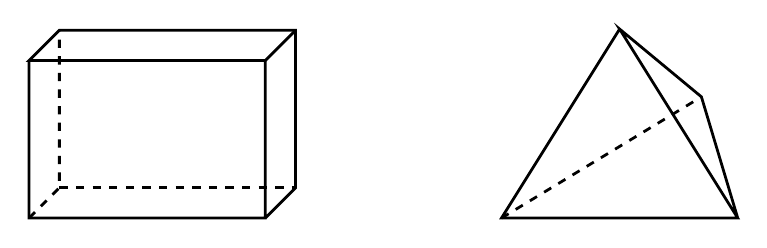
\begin{tikzpicture}[scale=2, line width=1pt]
\coordinate (A) at (0  ,0  ,0) ;
\coordinate (B) at (1.5,0  ,0) ;
\coordinate (C) at (1.5,1  ,0) ;
\coordinate (D) at (0  ,1  ,0) ;
\coordinate (E) at (0  ,0  ,-0.5) ;
\coordinate (F) at (1.5,0  ,-0.5) ;
\coordinate (G) at (1.5,1  ,-0.5) ;
\coordinate (H) at (0  ,1  ,-0.5) ;
\draw (D) -- (A) -- (B) -- (C) -- (D) -- (H) -- (G) -- (F) -- (B);
\draw (C) -- (G);
\draw [dashed] (A) -- (E) -- (H);
\draw [dashed] (E) -- (F);
\coordinate (I) at (3   ,0  ,0) ;
\coordinate (J) at (4.5 ,0  ,0) ;
\coordinate (K) at (3.75,1.2,0) ;
\coordinate (L) at (4   ,0.5,-0.7) ;
\draw[black] (K) -- (I) -- (J) -- (K) -- (L) -- (J) ;
\draw [dashed] (I) -- (L);
\end{tikzpicture}
\caption{3D allowed elements}
\label{3D_mesh}
\end{center}
\end{figure}
\end{itemize}

\textbf{Be carefull} non standard and hybrih meshing are not supported! (cf Figure \ref{hybr})

\begin{figure}[h!]
\begin{center}
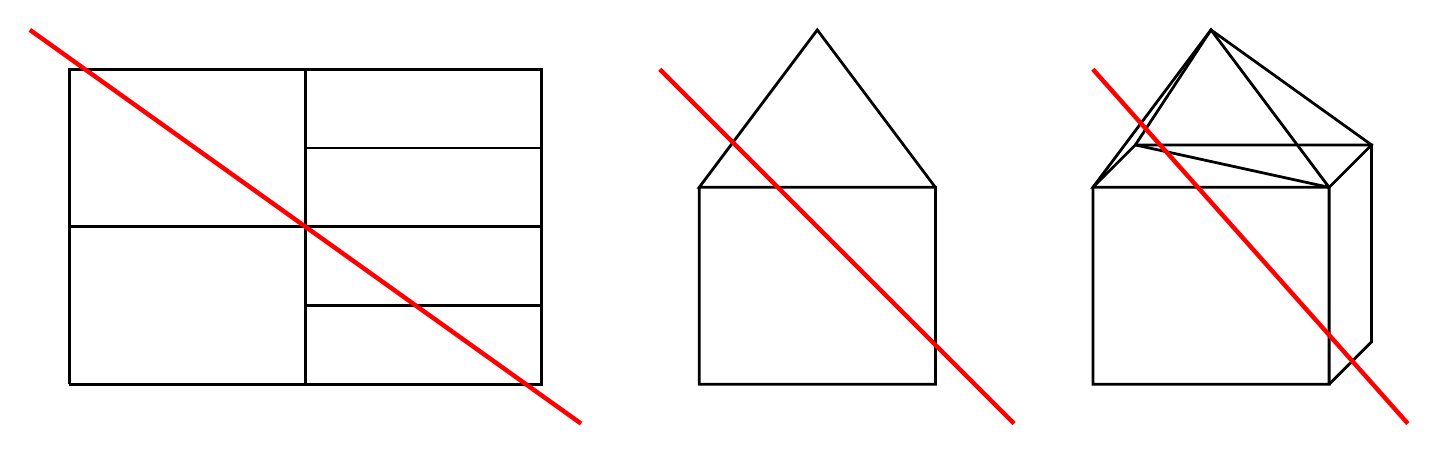
\begin{tikzpicture}[scale=2, line width=1pt]
\coordinate (A1) at (0,0) ;
\coordinate (A2) at (0,1) ;
\coordinate (A3) at (0,2) ;
\coordinate (B1) at (1.5,0  ) ;
\coordinate (B2) at (1.5,0.5) ;
\coordinate (B3) at (1.5,1  ) ;
\coordinate (B4) at (1.5,1.5) ;
\coordinate (B5) at (1.5,2  ) ;
\coordinate (C1) at (3,0  ) ;
\coordinate (C2) at (3,0.5) ;
\coordinate (C3) at (3,1  ) ;
\coordinate (C4) at (3,1.5) ;
\coordinate (C5) at (3,2  ) ;
\draw (A1) -- (C1) -- (C5) -- (A3) -- (A1);
\draw (A2) -- (C3);
\draw (B1) -- (B5);
\draw (B4) -- (C4);
\draw (B2) -- (C2);
\draw [ultra thick,red] (-0.25,2.25) -- (3.25,-0.25) ;

\coordinate (D1) at (4   ,0) ;
\coordinate (D2) at (5.5 ,0) ;
\coordinate (D3) at (5.5 ,1.25) ;
\coordinate (D4) at (4   ,1.25) ;
\coordinate (D5) at (4.75,2.25) ;
\draw (D4) -- (D1) -- (D2) -- (D3) -- (D4) -- (D5) -- (D3);
\draw [ultra thick,red] (3.75,2) -- (6,-0.25) ;

\coordinate (E1) at (6.5 ,0   ,0) ;
\coordinate (E2) at (8   ,0   ,0) ;
\coordinate (E3) at (8   ,1.25,0) ;
\coordinate (E4) at (6.5 ,1.25,0) ;
\coordinate (E5) at (7.25,2.25,0) ;
\coordinate (E6) at (8   ,0   ,-0.7) ;
\coordinate (E7) at (8   ,1.25,-0.7) ;
\coordinate (E8) at (6.5 ,1.25,-0.7) ;
\draw (E4) -- (E1) -- (E2) -- (E3) -- (E4) -- (E5) -- (E3);
\draw (E2) -- (E6) -- (E7) -- (E8) -- (E4);
\draw (E8) -- (E5) -- (E7) -- (E3) -- (E8);
\draw [ultra thick,red] (6.5,2) -- (8.5,-0.25) ;

\end{tikzpicture}
\caption{Prohibited meshes}
\label{hybr}
\end{center}
\end{figure}









%%%%%%%%%%%%%%%%%%%%%%%%%%%%%%%%%%%%%%
\subsection{Import mesh file}
%%%%%%%%%%%%%%%%%%%%%%%%%%%%%%%%%%%%%%
If your mesh was generated with an external tool like \href{http://www.salome-platform.org}{Salom\'e} (open source software), \href{http://resource.ansys.com/Products/Other+Products/ANSYS+ICEM+CFD}{ICEM} (commercial software), \href{http://gmsh.info/}{Gmsh} (open source software, included in \trust package) or \href{http://www-cast3m.cea.fr/}{Cast3M} (CEA software), then you must use one of the following keyword into your data file:

\begin{itemize}
\item \href{\REFERENCEMANUAL\#readmed}{\textbf{Read\_MED}} for a MED file from \href{http://www.salome-platform.org}{Salom\'e}, \href{http://gmsh.info/}{Gmsh},... ,
\item \href{\REFERENCEMANUAL\#readfile}{\textbf{Read\_File}} for a binary mesh file from \href{http://resource.ansys.com/Products/Other+Products/ANSYS+ICEM+CFD}{ICEM},
\item for another format, see the \href{\REFERENCEMANUAL\#read}{\trust Reference Manual}.
\end{itemize}

If you want to learn how to make a mesh with Salom\'e or Gmsh and read it with \trust, you can go to see the exercises of the \trust tutorial: \href{TRUST_tutorial.pdf\#salome}{here} for Salom\'e and \href{TRUST_tutorial.pdf\#gmsh}{here} for Gmsh.




%%%%%%%%%%%%%%%%%%%%%%%%%%%%%%%%%%%%%%
\subsection{Create quickly a mesh}
%%%%%%%%%%%%%%%%%%%%%%%%%%%%%%%%%%%%%%
Here is an example of a simple geometry (of non complex channel type) using the internal tool of \trust:
\begin{center}
\fbox{ \begin{minipage}[c]{0.9\textwidth}
\begin{alltt}
{\bf{Mailler}} \textit{my\_domain}

\{

\hspace{1cm}        \textcolor{blue}{/* Define the domain with one cavity */}

\hspace{1cm}        \textcolor{blue}{/* cavity 1m*2m with 5*22 cells */}

\hspace{1cm}        {\bf{Pave}} \textit{box}

\hspace{1cm}        \{

\hspace{2cm}            {\bf{Origine}} 0. 0.

\hspace{2cm}            {\bf{Longueurs}} 1 2

\hspace{2cm}            \textcolor{blue}{/* Cartesian grid */}

\hspace{2cm}            {\bf{Nombre\_de\_Noeuds}} 6 23

\hspace{2cm}            \textcolor{blue}{/* Uniform mesh */}

\hspace{2cm}            {\bf{Facteurs}} 1. 1.

\hspace{1cm}        \}

\hspace{1cm}        \{

\hspace{2cm}            \textcolor{blue}{/* Definition and names of boundary conditions */}

\hspace{2cm}            {\bf{bord}} \textit{Inlet}   \hspace{0.25cm} X = 0.  0. <= Y <= 2.

\hspace{2cm}            {\bf{bord}} \textit{Outlet}  \hspace{0.05cm} X = 1.  0. <= Y <= 2.

\hspace{2cm}            {\bf{bord}} \textit{Upper}   \hspace{0.25cm} Y = 2.  0. <= X <= 1.

\hspace{2cm}            {\bf{bord}} \textit{Lower}   \hspace{0.25cm} Y = 0.  0. <= X <= 1.

\hspace{1cm}        \}

\}
\end{alltt}
\end{minipage}}
\end{center}

To use this mesh in your data file, you just have to add the previous block in your data file or save it in a file named for example "\textit{my\_mesh.geo}" and add the line:\\
\begin{center}
\fbox{ \begin{minipage}[c]{0.5\textwidth}
\begin{alltt}
{\bf{Read\_file}} \textit{my\_mesh.geo} \textcolor{red}{{\bf{;}}}
\end{alltt}
\end{minipage}}
\end{center}

\underline{Do not forget the semi-colonn at the end of the line!}\\




%%%%%%%%%%%%%%%%%%%%%%%%%%%%%%%%%%%%%%
\subsection{Transform mesh within data file}
%%%%%%%%%%%%%%%%%%%%%%%%%%%%%%%%%%%%%%
You can also made transformations on your mesh after the \textbf{"Mailler"} or \textbf{"Read\_*"} command, using the following keywords:
\begin{itemize}
\item \href{\REFERENCEMANUAL\#triangulate}{\textbf{Trianguler}} to triangulate your 2D cells and create an unstructured mesh.
\item \href{\REFERENCEMANUAL\#tetraedriser}{\textbf{Tetraedriser}} to tetrahedralise 3D cells and create an unstructured mesh.
\item \href{\REFERENCEMANUAL\#raffineranisotrope}{\textbf{Raffiner\_anisotrope}}/\href{\REFERENCEMANUAL\#raffinerisotrope}{\textbf{Raffiner\_isotrope}} to triangulate/tetrahedralise elements of an untructured mesh.
\item \href{\REFERENCEMANUAL\#extrudebord}{\textbf{ExtrudeBord}} to generate an extruded mesh from a boundary of a tetrahedral or an hexahedral mesh. 
\Note that ExtrudeBord in VEF generates 3 or 14 tetrahedra from extruded prisms.
\item \href{\REFERENCEMANUAL\#regroupebord}{\textbf{RegroupeBord}} to build a new boundary with several boundaries of the domain.
\item \href{\REFERENCEMANUAL\#transformer}{\textbf{Transformer}} to transform the coordinates of the geometry.
\item for other commands, see the section \href{\REFERENCEMANUAL\#interprete}{interprete} of the \trust Reference Manual.
\end{itemize}

\Note that theses mesh modifications work on all mesh type (i.e. also for \textbf{*.geo} or \textbf{*.bin} or \textbf{*.med} files).



%%%%%%%%%%%%%%%%%%%%%%%%%%%%%%%%%%%%%%
\subsection{Test your mesh}
%%%%%%%%%%%%%%%%%%%%%%%%%%%%%%%%%%%%%%
The keyword \href{\REFERENCEMANUAL\#discretiserdomaine}{\textbf{Discretiser\_domaine}} is useful to discretize the domain (faces will be created) without defining a problem.
Indeed, you can create a minimal data file, post-process your mesh in lata format (for example) and visualize it with VisIt. \\

\Note that you must name all the boundaries!\\

Here is an example of this kind of data file:

\begin{center}
\fbox{ \begin{minipage}[c]{0.8\textwidth}
\begin{center}
\textbf{my\_data\_file.data}
\end{center}
\end{minipage}}
\fbox{ \begin{minipage}[c]{0.8\textwidth}
\begin{alltt}
{\bf{dimension 3}}

{\bf{Domaine}} \textit{my\_domain}

{\bf{Mailler}} \textit{my\_domain}

\{

\hspace{1cm}    {\bf{Pave}} \textit{box}

\hspace{1cm}    \{

\hspace{2cm}        {\bf{Origine}} 0. 0. 0.

\hspace{2cm}        {\bf{Longueurs}} 1 2 1

\hspace{2cm}        {\bf{Nombre\_de\_Noeuds}} 6 23 6

\hspace{2cm}        {\bf{Facteurs}} 1. 1. 1.

\hspace{1cm}    \}

\hspace{1cm}    \{

\hspace{2cm}        {\bf{bord}} \textit{Inlet}  \hspace{0.25cm} X = 0. 0. <= Y <= 2.  0. <= Z <= 1.

\hspace{2cm}        {\bf{bord}} \textit{Outlet} \hspace{0.05cm} X = 1.  0. <= Y <= 2.  0. <= Z <= 1.

\hspace{2cm}        {\bf{bord}} \textit{Upper}  \hspace{0.25cm} Y = 2.  0. <= X <= 1.  0. <= Z <= 1.

\hspace{2cm}        {\bf{bord}} \textit{Lower}  \hspace{0.25cm} Y = 0. 0. <= X <= 1.  0. <= Z <= 1.

\hspace{2cm}        {\bf{bord}} \textit{Front}  \hspace{0.25cm} Z = 0. 0. <= X <= 1.  0. <= Y <= 2.

\hspace{2cm}        {\bf{bord}} \textit{Back}   \hspace{0.45cm} Z = 1. 0. <= X <= 1.  0. <= Y <= 2.

\hspace{1cm}    \}

\}

{\bf{discretiser\_domaine}} \textit{my\_domain}

{\bf{postraiter\_domaine}} \{ {\bf{domaine}} \textit{my\_domain} {\bf{format lata}} \}

{\bf{End}}
    \end{alltt}
\end{minipage}}
\end{center}

To use it, launch in a bash terminal:
\begin{verbatim}
# if not already done
> source $my_path_to_TRUST_installation/env_TRUST.sh
# then
> trust my_data_file
> visit -o my_data_file.lata &
\end{verbatim}

To see how to use VisIt, go to see the first \trust tutorial exercise: \href{TRUST_tutorial.pdf\#exo1}{Obstacle}.\\

If you want to learn how to make a mesh with Salom\'e or Gmsh and read it with \trust, you can go to see the exercises of the \trust tutorial: \href{TRUST_tutorial.pdf\#salome}{here} for Salom\'e and \href{TRUST_tutorial.pdf\#gmsh}{here} for Gmsh.







%%%%%%%%%%%%%%%%%%%%%%%%%%%%%%%%%%%%%%%%%%%%%%%%%%%%%%%%%%%%%%%
\section{Discretization}
%%%%%%%%%%%%%%%%%%%%%%%%%%%%%%%%%%%%%%%%%%%%%%%%%%%%%%%%%%%%%%%
You have to specify the discretization type which can be \href{\REFERENCEMANUAL\#vdf}{\textbf{VDF}}, \href{\REFERENCEMANUAL\#ef}{\textbf{EF}} or \href{\REFERENCEMANUAL\#vefprep1b}{\textbf{VEFPreP1B}}.\\

In \textbf{VDF} discretization, the locations of the unknown are drawn in the Figure \ref{fig_VDF}.\\

\begin{figure}[h!]
\begin{center}
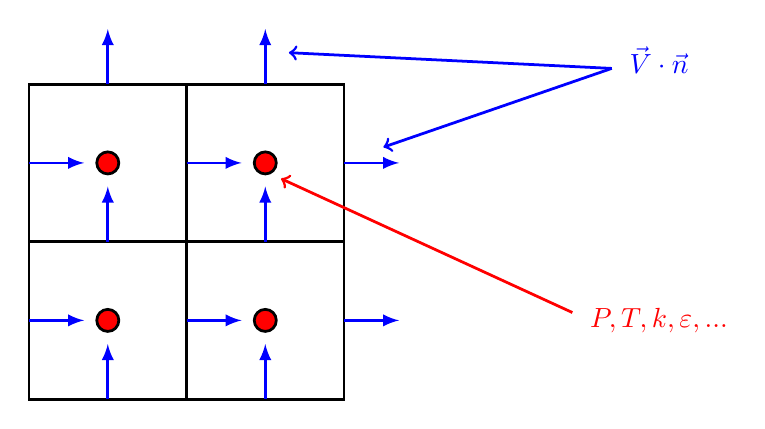
\begin{tikzpicture}[scale=2, line width=1pt]
\coordinate (A) at (0,0) ;
\coordinate (B) at (1,0) ;
\coordinate (C) at (2,0) ;
\coordinate (D) at (2,1) ;
\coordinate (E) at (2,2) ;
\coordinate (F) at (1,2) ;
\coordinate (G) at (0,2) ;
\coordinate (H) at (0,1) ;
\draw[black] (A) -- (C) -- (E) -- (G) -- cycle ;
\draw[black] (H) -- (D) ;
\draw[black] (F) -- (B) ;
\draw[black,fill=red] (0.5,0.5) circle (0.07);
\draw[black,fill=red] (1.5,0.5) circle (0.07);
\draw[black,fill=red] (0.5,1.5) circle (0.07);
\draw[black,fill=red] (1.5,1.5) circle (0.07);
\draw[blue] [->] [>=latex] (0.5,0) -- (0.5,0.35);
\draw[blue] [->] [>=latex] (0.5,1) -- (0.5,1.35);
\draw[blue] [->] [>=latex] (0.5,2) -- (0.5,2.35);
\draw[blue] [->] [>=latex] (1.5,0) -- (1.5,0.35);
\draw[blue] [->] [>=latex] (1.5,1) -- (1.5,1.35);
\draw[blue] [->] [>=latex] (1.5,2) -- (1.5,2.35);
\draw[blue] [->] [>=latex] (0,0.5) -- (0.35,0.5);
\draw[blue] [->] [>=latex] (1,0.5) -- (1.35,0.5);
\draw[blue] [->] [>=latex] (2,0.5) -- (2.35,0.5);
\draw[blue] [->] [>=latex] (0,1.5) -- (0.35,1.5);
\draw[blue] [->] [>=latex] (1,1.5) -- (1.35,1.5);
\draw[blue] [->] [>=latex] (2,1.5) -- (2.35,1.5);
\draw[blue] (4,2) node[above]{$\vec{V} \cdot \vec{n}$} ;
\draw[blue] [<-] (1.65,2.2) -- (3.7,2.1);
\draw[blue] [<-] (2.25,1.6) -- (3.7,2.1);
\draw[red] (4,0.5) node {$P, T, k, \varepsilon, ...$} ;
\draw[red] [<-] (1.6,1.4) -- (3.45,0.55);
\end{tikzpicture}
\caption{VDF unknown localisations}
\label{fig_VDF}
\end{center}
\end{figure}

For \textbf{VEFPreP1B}, the locations of the unknown are drawn in the Figure \ref{fig_VEF}.\\

\begin{figure}[h!]
\begin{center}
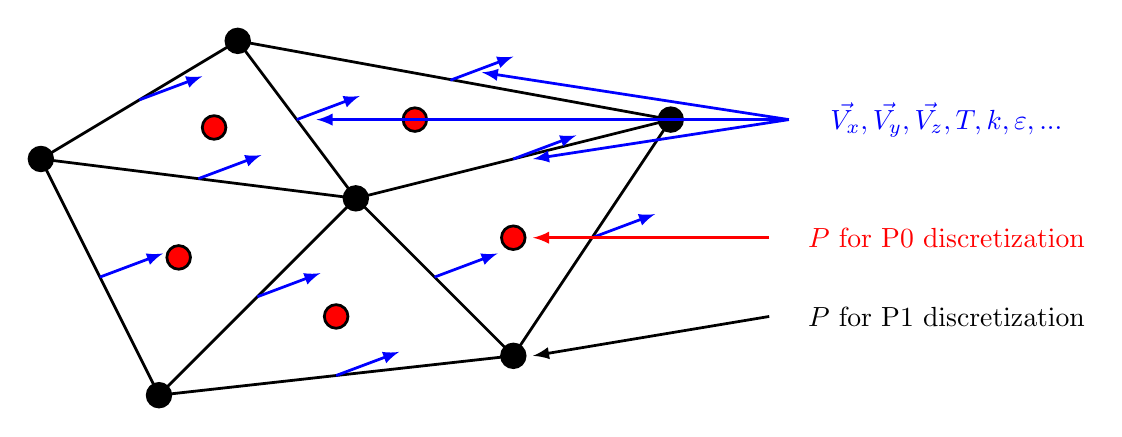
\begin{tikzpicture}[scale=1, line width=1pt]
\coordinate (A) at (1.5,0) ;
\coordinate (B) at (6,0.5) ;
\coordinate (C) at (8,3.5) ;
\coordinate (D) at (2.5,4.5) ;
\coordinate (E) at (0,3) ;
\coordinate (F) at (4,2.5) ;
\draw[black] (A) -- (B) -- (C) -- (D) -- (E) -- (A) -- (F) -- (B);
\draw[black] (C) -- (F) -- (D);
\draw[black] (E) -- (F);
\draw[black,fill=black] (A) circle (0.15);
\draw[black,fill=black] (B) circle (0.15);
\draw[black,fill=black] (C) circle (0.15);
\draw[black,fill=black] (D) circle (0.15);
\draw[black,fill=black] (E) circle (0.15);
\draw[black,fill=black] (F) circle (0.15);
\draw[black,fill=red] (3.75,1) circle (0.15);
\draw[black,fill=red] (6,2) circle (0.15);
\draw[black,fill=red] (4.75,3.5) circle (0.15);
\draw[black,fill=red] (2.2,3.4) circle (0.15);
\draw[black,fill=red] (1.75,1.75) circle (0.15);
\begin{scope}[xshift=5cm, yshift=1.5cm]
\draw[blue] [->] [>=latex] (0,0) -- (0.8,0.3);
\end{scope}
\begin{scope}[xshift=7cm, yshift=2cm]
\draw[blue] [->] [>=latex] (0,0) -- (0.8,0.3);
\end{scope}
\begin{scope}[xshift=5.2cm, yshift=4cm]
\draw[blue] [->] [>=latex] (0,0) -- (0.8,0.3);
\end{scope}
\begin{scope}[xshift=1.25cm, yshift=3.75cm]
\draw[blue] [->] [>=latex] (0,0) -- (0.8,0.3);
\end{scope}
\begin{scope}[xshift=0.75cm, yshift=1.5cm]
\draw[blue] [->] [>=latex] (0,0) -- (0.8,0.3);
\end{scope}
\begin{scope}[xshift=2.75cm, yshift=1.25cm]
\draw[blue] [->] [>=latex] (0,0) -- (0.8,0.3);
\end{scope}
\begin{scope}[xshift=3.75cm, yshift=0.25cm]
\draw[blue] [->] [>=latex] (0,0) -- (0.8,0.3);
\end{scope}
\begin{scope}[xshift=6cm, yshift=3cm]
\draw[blue] [->] [>=latex] (0,0) -- (0.8,0.3);
\end{scope}
\begin{scope}[xshift=3.25cm, yshift=3.5cm]
\draw[blue] [->] [>=latex] (0,0) -- (0.8,0.3);
\end{scope}
\begin{scope}[xshift=2cm, yshift=2.75cm]
\draw[blue] [->] [>=latex] (0,0) -- (0.8,0.3);
\end{scope}
\draw[blue] (11.5,3.5) node {$\vec{V_x}, \vec{V_y}, \vec{V_z}, T, k, \varepsilon, ...$} ;
\draw[blue] [->] [>=latex] (9.5,3.5) -- (5.6,4.1);
\draw[blue] [->] [>=latex] (9.5,3.5) -- (3.5,3.5);
\draw[blue] [->] [>=latex] (9.5,3.5) -- (6.25,3);
\draw[red] (11.5,2) node {$P$ for P0 discretization} ;
\draw[red] [->] [>=latex] (9.25,2) -- (6.25,2);
\draw[black] (11.5,1) node {$P$ for P1 discretization} ;
\draw[black] [->] [>=latex] (9.25,1) -- (6.25,0.5);
\end{tikzpicture}
\caption{VEF unknown localisations in 2D}
\label{fig_VEF}
\end{center}
\end{figure}

In 3D for the pressure, we can also use the P0+P1+Pa discretization for flow with a strong source term and a low velocity field.
In this case P0+P1 pressure gradient has trouble to match the source term so we use P0+P1+Pa discretization (cf Figure \ref{fig_VEF_pressure_loc}).

\begin{figure}[h!]
\begin{center}
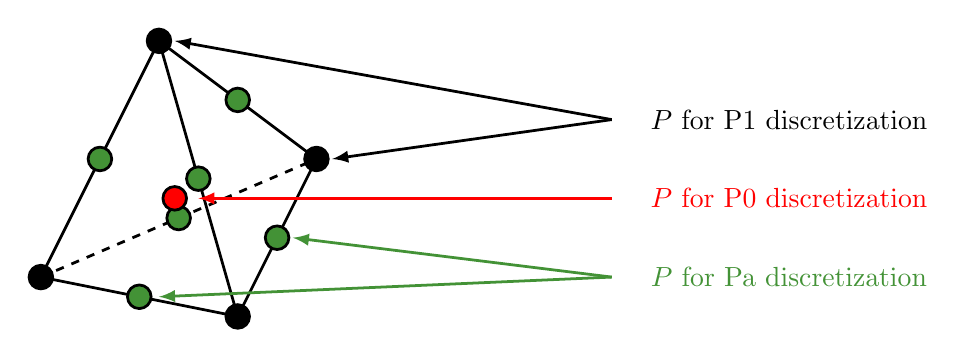
\begin{tikzpicture}[scale=1, line width=1pt]
\coordinate (A) at (0.5,1) ;
\coordinate (B) at (3,0.5) ;
\coordinate (C) at (4,2.5) ;
\coordinate (D) at (2,4) ;
\draw[black] (B) -- (C) -- (D) -- (A) -- (B) -- (D);
\draw[black,dashed] (A) -- (C);
\draw[black,fill=black] (A) circle (0.15);
\draw[black,fill=black] (B) circle (0.15);
\draw[black,fill=black] (C) circle (0.15);
\draw[black,fill=black] (D) circle (0.15);
\draw[black,fill=Greeen] (1.75,0.75) circle (0.15);
\draw[black,fill=Greeen] (3.5,1.5) circle (0.15);
\draw[black,fill=Greeen] (3,3.25) circle (0.15);
\draw[black,fill=Greeen] (1.25,2.5) circle (0.15);
\draw[black,fill=Greeen] (2.25,1.75) circle (0.15);
\draw[black,fill=Greeen] (2.5,2.25) circle (0.15);
\draw[black,fill=red] (2.2,2) circle (0.15);
\draw[black] (10,3) node {$P$ for P1 discretization} ;
\draw[black] [->] [>=latex] (7.75,3) -- (2.2,4);
\draw[black] [->] [>=latex] (7.75,3) -- (4.2,2.5);
\draw[red] (10,2) node {$P$ for P0 discretization} ;
\draw[red] [->] [>=latex] (7.75,2) -- (2.5,2);
\draw[Greeen] (10,1) node {$P$ for Pa discretization} ;
\draw[Greeen] [->] [>=latex] (7.75,1) -- (3.7,1.5);
\draw[Greeen] [->] [>=latex] (7.75,1) -- (2,0.75);
\end{tikzpicture}
\caption{VEF pressure localisation in 3D}
\label{fig_VEF_pressure_loc}
\end{center}
\end{figure}

To specify the wanted discretization, you have to add the following block to your data file:

    \begin{center}
    \fbox{ \begin{minipage}[c]{0.5\textwidth}
    \begin{alltt}
    \textit{{\bf{Discretization\_type}} my\_discretization}

    [{\bf{Read }} \textit{my\_discretization \{ ... \}}]
    \end{alltt}
    \end{minipage}}
    \end{center}

You can add parameters to your discretization with the optional keyword \href{\REFERENCEMANUAL\#read}{\textbf{Read}} (see \href{\REFERENCEMANUAL\#vefprep1b}{\textbf{VEFPreP1B discretization}}).

On the \href{http://www-trio-u.cea.fr/scripts/home/publigen/content/templates/show.asp?L=EN&P=55&vTicker=alleza&ITEMID=3}{TRUST website}, you can find information about:
\begin{itemize}
\item \textbf{VDF} discretization in the \href{http://www-trio-u.cea.fr/home/liblocal/docs/Theses/these_chatelain_2004.pdf}{PhD thesis of A. Chatelain},
\item \textbf{VEFPreP1B} discretization (Crouzet-Raviart elements) in the \href{http://www-trio-u.cea.fr/home/liblocal/docs/Theses/these_fortin_2006.pdf}{PhD thesis of T. Fortin} and \href{http://www-trio-u.cea.fr/home/liblocal/docs/Theses/These_Heib_2003.pdf}{PhD thesis of S. Heib}.
\end{itemize}


%%%%%%%%%%%%%%%%%%%%%%%%%%%%%%%%%%%%%%%%%%%%%%%%%%%%%%%%%%%%%%%
\section{Time schemes}
%%%%%%%%%%%%%%%%%%%%%%%%%%%%%%%%%%%%%%%%%%%%%%%%%%%%%%%%%%%%%%%
Now you can choose your time scheme to solve your problem. For this you must
specify the time scheme type wanted and give it a name. 
then you have to specify its parameters by filling the associated \textbf{"Read"} block.

    \begin{center}
    \fbox{ \begin{minipage}[c]{0.5\textwidth}
    \begin{alltt}
    {\bf{\textit{Scheme\_type}}} \textit{my\_time\_scheme}

    {\bf{Read}} \textit{my\_time\_scheme} \{ ... \}
    \end{alltt}
    \end{minipage}}
    \end{center}

%%%%%%%%%%%%%%%%%%%%%%%%%%%%%%%%%%%%%%
\subsection{Some available time schemes}
%%%%%%%%%%%%%%%%%%%%%%%%%%%%%%%%%%%%%%
%Here are some \href[page=DOCLINK_TIME SCHEMES]{\REFERENCEMANUAL}{available types of explicit schemes}:
Here are some available types of explicit schemes:
\begin{itemize}
\item \href{\REFERENCEMANUAL\#eulerscheme}{\textbf{Scheme\_Euler\_explicit}},
\item \href{\REFERENCEMANUAL\#schemaadamsbashforthorder2}{\textbf{Schema\_Adams\_Bashforth\_order\_2}},
%\item \textbf{Schema\_Adams\_Bashforth\_order\_3}
%\item \textbf{Runge\_Kutta\_Rationnel\_ordre\_2}
\item \href{\REFERENCEMANUAL\#rungekuttaordre3}{\textbf{Runge\_Kutta\_ordre\_3}},
%\item \textbf{Runge\_Kutta\_ordre\_4\_D3P}
%\item \textbf{Schema\_Predictor\_Corrector}
%\item \textbf{Sch\_CN\_iteratif}
%\item \textbf{Sch\_CN\_EX\_iteratif}
%\item \textbf{Schema\_Phase\_Field}
%\item \textbf{RK3\_FT}
\end{itemize}

%And also some \href[page=DOCLINK_TIME SCHEMES]{\REFERENCEMANUAL}{available types of implicit schemes}:
And also some available types of implicit schemes:
\begin{itemize}
\item \href{\REFERENCEMANUAL\#schemaeulerimplicite}{\textbf{Scheme\_Euler\_implicit}},
%\item \textbf{Schema\_Adams\_Moulton\_order\_2}
\item \href{\REFERENCEMANUAL\#schemaadamsmoultonorder3}{\textbf{Schema\_Adams\_Moulton\_order\_3}}.
%\item \textbf{Schema\_Backward\_Differentiation\_order\_2}
%\item \textbf{Schema\_Backward\_Differentiation\_order\_3}
\end{itemize}

For other scheme, see \href{\REFERENCEMANUAL\#schematempsbase}{this section} of the Reference Manual.\\

\Note that you can use semi-implicit schemes activating the \textbf{diffusion\_implicite} keyword in your explicit time scheme.



%%%%%%%%%%%%%%%%%%%%%%%%%%%%%%%%%%%%%%
\subsection{Calculation stopping condition}
%%%%%%%%%%%%%%%%%%%%%%%%%%%%%%%%%%%%%%
You must specify at least one stopping condition for you simulation.
It can be:
\begin{itemize}
\item the final time: \textbf{tmax}
\item the maximal allowed cpu time: \textbf{tcpumax}
\item the number of time step: \textbf{nb\_pas\_dt\_max}
\item the convergency treshold: \textbf{seuil\_statio}
\end{itemize}

\Note that if the time step wants to go under the minimal time step \textbf{dt\_min}, \trust will stop the calculation.\\

If you want to stop properly your running calculation (i.e. with all saves), you may use the \textit{my\_data\_file}.stop file (cf section \ref{stopfile}).
When the simulation is running, you can see the "\textbf{0}" value in that file.\\

To stop it, put a "\textbf{1}" instead of the "\textbf{0}" and at the next iteration the calculation will stop properly.\\

When you don't change any thing to that file, at the end of the calculation, you can see that it is writen "\textbf{Finished correctly}".


%%%%%%%%%%%%%%%%%%%%%%%%%%%%%%%%%%%%%%%%%%%%%%%%%%%%%%%%%%%%%%%
\section{Medium/Type of fluide}
%%%%%%%%%%%%%%%%%%%%%%%%%%%%%%%%%%%%%%%%%%%%%%%%%%%%%%%%%%%%%%%
To specify the medium or fluid, you may add the following block.

    \begin{center}
    \fbox{ \begin{minipage}[c]{0.5\textwidth}
    \begin{alltt}
    {\bf{\textit{Fluid\_type}}} \textit{my\_medium}

    {\bf{Read}} \textit{my\_medium} \{ ... \}
    \end{alltt}
    \end{minipage}}
    \end{center}

{\bf{\textit{Fluid\_type}}} can be one of the following:
\begin{itemize}
\item \href{\REFERENCEMANUAL\#fluideincompressible}{\textbf{Fluide\_incompressible}}
\item \href{\REFERENCEMANUAL\#fluidequasicompressible}{\textbf{Fluide\_quasi\_compressible}}
%\item \textbf{Fluide\_Ostwald}
%\item \textbf{Constituant}
\item \href{\REFERENCEMANUAL\#solide}{\textbf{Solide}}
\item for other types and more information see \href{\REFERENCEMANUAL\#milieubase}{\trust Reference Manual}.
\end{itemize}

If you want to use more than one medium, you can add an other block for each medium or fluid.\\





%%%%%%%%%%%%%%%%%%%%%%%%%%%%%%%%%%%%%%%%%%%%%%%%%%%%%%%%%%%%%%%
\section{Add gravity}
%%%%%%%%%%%%%%%%%%%%%%%%%%%%%%%%%%%%%%%%%%%%%%%%%%%%%%%%%%%%%%%
If needed, you can add gravity term to your simulation. This is done by adding
a uniform field, no matter his name. For example in 2D:

    \begin{center}
    \fbox{ \begin{minipage}[c]{0.5\textwidth}
    \begin{alltt}
    \textcolor{blue}{\# Gavity vector definition \#}

    {\bf{Uniform\_field}} \textit{my\_gravity}

    {\bf{Read}} \textit{my\_gravity 2 0 -9.81}

    \end{alltt}
    \end{minipage}}
    \end{center}




%%%%%%%%%%%%%%%%%%%%%%%%%%%%%%%%%%%%%%%%%%%%%%%%%%%%%%%%%%%%%%%
\section{Objects association and discretization}
%%%%%%%%%%%%%%%%%%%%%%%%%%%%%%%%%%%%%%%%%%%%%%%%%%%%%%%%%%%%%%%
%%%%%%%%%%%%%%%%%%%%%%%%%%%%%%%%%%%%%%
\subsection{Association}
%%%%%%%%%%%%%%%%%%%%%%%%%%%%%%%%%%%%%%
Until now, we have created some objects, now we must associate them together.
For this, we must use the \href{\REFERENCEMANUAL\#associate}{\textbf{Associate}} interpretor:
    \begin{center}
    \fbox{ \begin{minipage}[c]{0.7\textwidth}
    \begin{alltt}
    \textcolor{blue}{\# Association between the different objects \#}

    {\bf{Associate}} \textit{my\_problem my\_domain}

    {\bf{Associate}} \textit{my\_problem my\_time\_scheme}

    {\bf{Associate}} \textit{my\_problem my\_medium}

    [{\bf{Associate}} \textit{my\_medium my\_gravity}]
    \end{alltt}
    \end{minipage}}
    \end{center}




%%%%%%%%%%%%%%%%%%%%%%%%%%%%%%%%%%%%%%
\subsection{Discretization}
%%%%%%%%%%%%%%%%%%%%%%%%%%%%%%%%%%%%%%
Then you must discretize your domain using the \href{\REFERENCEMANUAL\#discretize}{\textbf{Discretize}} interpretor:
    \begin{center}
    \fbox{ \begin{minipage}[c]{0.7\textwidth}
    \begin{alltt}
    {\bf{Discretize}}  \textit{my\_problem  my\_discretization}
    \end{alltt}
    \end{minipage}}
    \end{center}

The problem \textit{my\_problem} is discretized according to the \textit{my\_discretization} discretization.\\

IMPORTANT: A number of objects must be already associated (a domain, time scheme, central object) prior to invoking the \textbf{Discretize} keyword. The physical properties of this central object must also have been read.\\

\Note that when \trust succed the discretization step, the mesh is then validated by the code.\\

At this level of your data file, you can visualize your mesh with the "\textbf{-mesh}" option of the trust script, it will directly open your mesh with VisIt.
\begin{verbatim}
# if not already done
> source $my_path_to_TRUST_installation/env_TRUST.sh
# then
> trust -mesh my_data_file
\end{verbatim}
It will only run the mesh and stop, the problem will not be solved.




%%%%%%%%%%%%%%%%%%%%%%%%%%%%%%%%%%%%%%%%%%%%%%%%%%%%%%%%%%%%%%%%%%%%%%%%



%%%%%%%%%%%%%%%%%%%%%%%%%%%%%%%%%%%%%%%%%%%%%%%%%%%%%%%%%%%%%%%%%%%%%%%%
%
\chapter{Problem definition}
%
%%%%%%%%%%%%%%%%%%%%%%%%%%%%%%%%%%%%%%%%%%%%%%%%%%%%%%%%%%%%%%%%%%%%%%%%
%%%%%%%%%%%%%%%%%%%%%%%%%%%%%%%%%%%%%%%%%
\section{Set of equations}
%%%%%%%%%%%%%%%%%%%%%%%%%%%%%%%%%%%%%%%%%
In function of your choice of problem type, you will have a different set of equations.

%%%%%%%%%%%%%%%%%%%%%%%%%%%%%%%%%%%%%%
\subsection{Incompressible problems}
%%%%%%%%%%%%%%%%%%%%%%%%%%%%%%%%%%%%%%
\trust solves Navier-Stokes equations with/without heat equation for incompressible fluid:

$$
\left\{
\begin{array}{c}
\nabla \cdot \vec u =0 \\
\displaystyle{\frac{\partial \vec u }{\partial t} + \textcolor{red}{\nabla \cdot (\vec u \otimes \vec u)} = \textcolor{blue}{\nabla \cdot (\nu \nabla \vec u)} - \nabla P^* } \\
\displaystyle{\frac{\partial T}{\partial t} + \textcolor{red}{\vec u \nabla T} = \textcolor{blue}{\nabla \cdot (\alpha \nabla T)} + \frac{Q}{\rho C_p}}
\end{array}
\right.
$$

where: $\displaystyle{P^*=\frac{P}{\rho} + g z}$, $Q$ is a heat source term, and:

\begin{itemize}
\item $\rho$: density,
\item $\mu$: dynamic viscosity,
\item $\displaystyle{\nu=\frac{\mu}{\rho}}$: cinematic viscosity,
\item $\vec g=g z$: gravity vector in cartesian coordinates,
\item $\displaystyle{\alpha=\frac{\lambda}{\rho C_p}}$: thermal diffusivity.
\item $C_p$: specific heat capacity at constant pressure,
\item $\lambda$: thermal conductivity,
\end{itemize}

\Note that \textcolor{red}{red} terms are convective terms and \textcolor{blue}{blue} terms are diffusive terms.\\

\begin{center}
\fbox{ \begin{minipage}[c]{0.98\textwidth}
\begin{alltt}
{\bf{Pb\_\textcolor{magenta}{Thermo}hydraulique\textcolor{darkblue}{\_Concentration}\hspace{-0.15cm}\textcolor{Greeen}{\_Turbulent} } } \textit{my\_problem}

...

{\bf{Read}} \textit{my\_problem}

\{

\hspace{1cm}    \textcolor{blue}{\# Navier Stokes equations with/without turbulent model \#}

\hspace{1cm}    {\bf{Navier\_Stokes$\overbrace{\mbox{\_Standard}}^{\mbox{\textcolor{Greeen}{\_Turbulent}}}$} }

\hspace{1cm}    \{

\hspace{2cm}        {\bf{Solveur\_Pression}} \textit{my\_solver} \{ ... \}

\hspace{2cm}        {\bf{Diffusion}} \{ ... \}

\hspace{2cm}        {\bf{Convection}} \{ ... \}

\hspace{2cm}        {\bf{Initial\_conditions}} \{ ... \}

\hspace{2cm}        {\bf{Boundary\_conditions}} \{ ... \}

\hspace{2cm}        {\bf{\textcolor{Greeen}{Modele\_turbulence \textit{modele} \{ ... \} } }}

\hspace{2cm}        [{\bf{Sources}} \{ ... \}]

\hspace{2cm}       ...

\hspace{1cm}    \}

\hspace{1cm}    \textcolor{blue}{\# Energy equation with/without turbulent model \#}

\hspace{1cm}    {\bf{\textcolor{magenta}{Convection\_Diffusion\_Temperature}\textcolor{Greeen}{\_Turbulent}}}

\hspace{1cm}    \textcolor{magenta}{\{}

\hspace{2cm}        \textcolor{magenta}{{\bf{Diffusion}} \{ ... \}}

\hspace{2cm}        \textcolor{magenta}{{\bf{Convection}} \{ ... \}}

\hspace{2cm}        \textcolor{magenta}{{\bf{Initial\_conditions}} \{ ... \}}

\hspace{2cm}        \textcolor{magenta}{{\bf{Boundary\_conditions}} \{ ... \}}

\hspace{2cm}        \textcolor{magenta}{{\bf{\textcolor{Greeen}{Modele\_turbulence Prandtl \{ ... \} } }}}

\hspace{2cm}        \textcolor{magenta}{[{\bf{Sources}} \{ ... \}]}

\hspace{2cm}        \textcolor{magenta}{...}

\hspace{1cm}    \textcolor{magenta}{\}}

\hspace{1cm}    \textcolor{blue}{\# Constituent transportation equations with/without turbulent model \#}

\hspace{1cm}    {\bf{\textcolor{darkblue}{Convection\_Diffusion\_Concentration}\textcolor{Greeen}{\_Turbulent}}}

\hspace{1cm}    \textcolor{darkblue}{\{}

\hspace{2cm}        \textcolor{darkblue}{{\bf{Diffusion}} \{ ... \}}

\hspace{2cm}        \textcolor{darkblue}{{\bf{Convection}} \{ ... \}}

\hspace{2cm}        \textcolor{darkblue}{{\bf{Initial\_conditions}} \{ ... \}}

\hspace{2cm}        \textcolor{darkblue}{{\bf{Boundary\_conditions}} \{ ... \}}

\hspace{2cm}        \textcolor{darkblue}{{\bf{\textcolor{Greeen}{Modele\_turbulence Schmidt \{ ... \} } }}}

\hspace{2cm}        \textcolor{darkblue}{[{\bf{Sources}} \{ ... \}]}

\hspace{2cm}        \textcolor{darkblue}{...}

\hspace{1cm}    \textcolor{darkblue}{\}}

\}
\end{alltt}
\end{minipage}}
\end{center}

For documentation, see:\\

\begin{longtable}{|c|c|c|c|c|}
\hline
Thermo & hydraulique & Concentration & Turbulent & Reference Manual\tabularnewline
\hline 
\hline 
            & \textbf{Pb\_hydraulique}  &   
            &                           & \href{../../Outils/TRIOXDATA/XTriou/doc.pdf\#pbhydraulique}{doc} \tabularnewline 
\hline
            & \textbf{Pb\_hydraulique}  & \textbf{\textcolor{darkblue}{\_Concentration}}
            &                           & \href{../../Outils/TRIOXDATA/XTriou/doc.pdf\#pbhydrauliqueconcentration}{doc} \tabularnewline
\hline
            & \textbf{Pb\_hydraulique}  &   
            & \textbf{\textcolor{Greeen}{\_Turbulent}}      & \href{../../Outils/TRIOXDATA/XTriou/doc.pdf\#pbhydrauliqueturbulent}{doc} \tabularnewline
\hline
            & \textbf{Pb\_hydraulique}  & \textbf{\textcolor{darkblue}{\_Concentration}}
            & \textbf{\textcolor{Greeen}{\_Turbulent}}      & \href{../../Outils/TRIOXDATA/XTriou/doc.pdf\#pbhydrauliqueconcentrationturbulent}{doc} \tabularnewline
\hline
\textbf{Pb\_\textcolor{magenta}{Thermo}}     & \textbf{hydraulique}  &   
                        &                       & \href{../../Outils/TRIOXDATA/XTriou/doc.pdf\#pbthermohydraulique}{doc} \tabularnewline
\hline
\textbf{Pb\_\textcolor{magenta}{Thermo}}     & \textbf{hydraulique}  & \textbf{\textcolor{darkblue}{\_Concentration}}
                        &                       & \href{../../Outils/TRIOXDATA/XTriou/doc.pdf\#pbthermohydrauliqueconcentration}{doc} \tabularnewline
\hline
\textbf{Pb\_\textcolor{magenta}{Thermo}}     & \textbf{hydraulique}  &   
                        & \textbf{\textcolor{Greeen}{\_Turbulent}}  & \href{../../Outils/TRIOXDATA/XTriou/doc.pdf\#pbthermohydrauliqueturbulent}{doc} \tabularnewline
\hline
\textbf{Pb\_\textcolor{magenta}{Thermo}}     & \textbf{hydraulique}  & \textbf{\textcolor{darkblue}{\_Concentration}}
                        & \textbf{\textcolor{Greeen}{\_Turbulent}}  & \href{../../Outils/TRIOXDATA/XTriou/doc.pdf\#pbthermohydrauliqueconcentrationturbulent}{doc} \tabularnewline
\hline
\end{longtable}

\vspace{0.5cm}


%%%%%%%%%%%%%%%%%%%%%%%%%%%%%%%%%%%%%%
\subsection{Quasi-compressible problem}
%%%%%%%%%%%%%%%%%%%%%%%%%%%%%%%%%%%%%%
\trust solves Navier-Stokes equations with/without heat equation for quasi-compressible fluid:

$$
\left\{
\begin{array}{c}
\displaystyle{\frac{\partial \rho }{\partial t} + \nabla \cdot (\rho \vec u) =0 }\\
\displaystyle{ \frac{\partial \rho u}{\partial t} + \textcolor{red}{\nabla \cdot (\rho u u)} =  \textcolor{blue}{\nabla \cdot \left(\mu \nabla \vec u \right)} - \nabla P -\rho \vec g }\\
\displaystyle{ \rho C_p \left( \frac{\partial T}{\partial t} + \textcolor{red}{\vec u \nabla T} \right) = \textcolor{blue}{\nabla \cdot \left(\lambda \nabla T\right)} + \frac{dP_0}{dt} + Q }
\end{array}
\right.
$$

where: $P_0=\rho R T$, $Q$ is a heat source term, and:

\begin{itemize}
\item $\rho$: density,
\item $\mu$: dynamic viscosity,
\item $\displaystyle{\nu=\frac{\mu}{\rho}}$: cinematic viscosity,
\item $\vec g=g z$: gravity vector in cartesian coordinates,
\item $C_p$: specific heat capacity at constant pressure,
\item $\lambda$: thermal conductivity,
\item $\displaystyle{\alpha=\frac{\lambda}{\rho C_p}}$: thermal diffusivity.
\end{itemize}

\Note that \textcolor{red}{red} terms are convective terms and \textcolor{blue}{blue} terms are diffusive terms.\\


\begin{center}
\fbox{ \begin{minipage}[c]{0.95\textwidth}
\begin{alltt}
{\bf{Pb\_Thermohydraulique\textcolor{Greeen}{\_Turbulent}\_QC} } \textit{my\_problem}

...

{\bf{Read}} \textit{my\_problem}

\{

\hspace{1cm}    \textcolor{blue}{\# Navier Stokes equations for quasi-compressible fluid under \#}

\hspace{1cm}    \textcolor{blue}{\# low Mach numbers with/without turbulent model \#}

\hspace{1cm}    {\bf{Navier\_Stokes\textcolor{Greeen}{\_Turbulent}\_QC}}

\hspace{1cm}    \{

\hspace{2cm}        {\bf{Solveur\_Pression}} \textit{my\_solver} \{ ... \}

\hspace{2cm}        {\bf{Diffusion}} \{ ... \}

\hspace{2cm}        {\bf{Convection}} \{ ... \}

\hspace{2cm}        {\bf{Initial\_conditions}} \{ ... \}

\hspace{2cm}        {\bf{Boundary\_conditions}} \{ ... \}

\hspace{2cm}        {\bf{\textcolor{Greeen}{Modele\_turbulence \textit{modele} \{ ... \} } }}

\hspace{2cm}        [{\bf{Sources}} \{ ... \}]

\hspace{2cm}       ...

\hspace{1cm}    \}

\hspace{1cm}    \textcolor{blue}{\# Energy equation for quasi-compressible fluid under low Mach \#}

\hspace{1cm}    \textcolor{blue}{\# numbers with/without turbulent model \#}

\hspace{1cm}    {\bf{Convection\_Diffusion\_Chaleur}\textcolor{Greeen}{\_Turbulent}}

\hspace{1cm}    \{

\hspace{2cm}        {\bf{Diffusion}} \{ ... \}

\hspace{2cm}        {\bf{Convection}} \{ ... \}

\hspace{2cm}        {\bf{Initial\_conditions}} \{ ... \}

\hspace{2cm}        {\bf{Boundary\_conditions}} \{ ... \}

\hspace{2cm}        {\bf{\textcolor{Greeen}{Modele\_turbulence Prandtl \{ ... \} } }}

\hspace{2cm}        [{\bf{Sources}} \{ ... \}]

\hspace{2cm}        ...

\hspace{1cm}    \}

\}
\end{alltt}
\end{minipage}}
\end{center}

For more information on thermohydraulique QC problem, go \href{../../Outils/TRIOXDATA/XTriou/doc.pdf\#pbthermohydrauliqueqc}{here} and for thermohydraulique turbulent QC problem, go \href{../../Outils/TRIOXDATA/XTriou/doc.pdf\#pbthermohydrauliqueturbulentqc}{there}.



%%%%%%%%%%%%%%%%%%%%%%%%%%%%%%%%%%%%%%
\subsection{Conduction problem}
%%%%%%%%%%%%%%%%%%%%%%%%%%%%%%%%%%%%%%
For this kind of problem, \trust solves the heat equation:
$$
\rho C_p \frac{\partial T}{\partial t} = \textcolor{blue}{\nabla \cdot \left(\lambda \nabla T\right)} + Q
$$
where:
\begin{itemize}
\item $\rho$: density,
\item $C_p$: specific heat capacity at constant pressure,
\item $\lambda$: thermal conductivity,
\item $Q$ is a heat source term.
\end{itemize}

\Note that \textcolor{red}{red} terms are convective terms and \textcolor{blue}{blue} terms are diffusive terms.\\

In your data file, you will have:

\begin{center}
\fbox{ \begin{minipage}[c]{0.95\textwidth}
\begin{alltt}
{\bf{Pb\_Conduction} } \textit{my\_problem}

...

{\bf{Read}} \textit{my\_problem}

\{

\hspace{1cm}    \textcolor{blue}{\# Resolution of the heat equation \#}

\hspace{1cm}    {\bf{Conduction}}

\hspace{1cm}    \{

\hspace{2cm}        {\bf{Diffusion}} \{ ... \}

\hspace{2cm}        {\bf{Convection}} \{ ... \}

\hspace{2cm}        {\bf{Initial\_conditions}} \{ ... \}

\hspace{2cm}        {\bf{Boundary\_conditions}} \{ ... \}

\hspace{2cm}        [{\bf{Sources}} \{ ... \}]

\hspace{2cm}        ...

\hspace{1cm}    \}

\}
\end{alltt}
\end{minipage}}
\end{center}

For more information, see the \href{../../Outils/TRIOXDATA/XTriou/doc.pdf\#pbconduction}{\trust Reference Manual}.

%%%%%%%%%%%%%%%%%%%%%%%%%%%%%%%%%%%%%%
\subsection{Coupled problems}
%%%%%%%%%%%%%%%%%%%%%%%%%%%%%%%%%%%%%%
With \trust, we can couple problems. We will explain here the method for two problems
but you can couple as many problems as you want.\\

To couple two problems, we define two problems \textit{my\_problem\_1} and \textit{my\_problem\_2} each one associated to a separate domain \textit{my\_domain\_1} and \textit{my\_domain\_2}, and to a separate medium \textit{my\_medium\_1} and \textit{my\_medium\_2} (associated or not to the gravity).
\begin{center}
\fbox{ \begin{minipage}[c]{0.95\textwidth}
\begin{alltt}
{\bf{Dimension}} 2


{\bf{Pb_ThermoHydraulique_Turbulent}} \textit{my\_problem\_1}

{\bf{Pb_ThermoHydraulique_Turbulent}} \textit{my\_problem\_2}


{\bf{Domaine}} \textit{my\_domain\_1}

{\bf{Read\_file}} \textit{my\_mesh\_1.geo} ;


{\bf{Domaine}} \textit{my\_domain\_2}

{\bf{Read\_file}} \textit{my\_mesh\_2.geo} ;


{\bf{Fluide_Incompressible}} \textit{my\_medium\_1}

{\bf{Read}} \textit{my\_medium\_1} \{ ... \}


{\bf{Fluide_Incompressible}} \textit{my\_medium\_2}

{\bf{Read}} \textit{my\_medium\_2} \{ ... \}


{\bf{Associate}} \textit{my\_problem\_1} \textit{my\_domain\_1}

{\bf{Associate}} \textit{my\_problem\_1} \textit{my\_medium\_1}


{\bf{Associate}} \textit{my\_problem\_2} \textit{my\_domain\_2}

{\bf{Associate}} \textit{my\_problem\_2} \textit{my\_medium\_2}
\end{alltt}
\end{minipage}}
\end{center}


Then we define a coupled problem associated to a single time scheme like for example:
\begin{center}
\fbox{ \begin{minipage}[c]{0.95\textwidth}
\begin{alltt}
{\bf{Probleme\_Couple}} \textit{my\_coupled\_problem}


{\bf{VEFPreP1B}} \textit{my\_discretization}


{\bf{Scheme\_euler\_explicit}} \textit{my\_scheme}

{\bf{Read}} \textit{my\_scheme} \{ ... \}


{\bf{Associate}} \textit{my\_coupled\_problem} \textit{my\_problem\_1}

{\bf{Associate}} \textit{my\_coupled\_problem} \textit{my\_problem\_2}

{\bf{Associate}} \textit{my\_coupled\_problem} \textit{my\_scheme}
\end{alltt}
\end{minipage}}
\end{center}

Then we discretize and solve everything:
\begin{center}
\fbox{ \begin{minipage}[c]{0.95\textwidth}
\begin{alltt}
{\bf{Discretize}} \textit{my\_coupled\_problem} \textit{my\_discretization}

{\bf{Read}} \textit{my\_problem\_1} \{ ... \}

{\bf{Read}} \textit{my\_problem\_2} \{ ... \}

{\bf{Solve}} \textit{my\_coupled\_problem}

{\bf{End}}
\end{alltt}
\end{minipage}}
\end{center}

You can see the documentation of this kind of problem in the \href{../../Outils/TRIOXDATA/XTriou/doc.pdf\#coupledproblem}{\trust Reference Manual}.



%%%%%%%%%%%%%%%%%%%%%%%%%%%%%%%%%%%%%%
\subsection{Other problems}
%%%%%%%%%%%%%%%%%%%%%%%%%%%%%%%%%%%%%%
\trust can also solve the following types of problems:
\begin{itemize}
%\item \href{../../Outils/TRIOXDATA/XTriou/doc.pdf\#problemeftdiscgen}{Front-Tracking problems},
%\item \href{../../Outils/TRIOXDATA/XTriou/doc.pdf\#pbphasefield}{Problems to solve local instantaneous incompressible-two-phase-flows},
\item \href{../../Outils/TRIOXDATA/XTriou/doc.pdf\#pbthermohydrauliqueconcentrationscalairespassifs}{Resolution of NAVIER STOKES/energy/multiple constituent transportation equations, with the additional passive scalar equations}, and
\item \href{../../Outils/TRIOXDATA/XTriou/doc.pdf\#chimie}{describe the chemical reactions}.
\end{itemize}



%%%%%%%%%%%%%%%%%%%%%%%%%%%%%%%%%%%%%%%%%
\section{Pressure solvers}
%%%%%%%%%%%%%%%%%%%%%%%%%%%%%%%%%%%%%%%%%
Then you may indicate the choice of pressure solver (cf \href{../../Outils/TRIOXDATA/XTriou/doc.pdf\#solveursysbase}{\trust Reference Manual}) using the following syntaxe:
    \begin{center}
    \fbox{ \begin{minipage}[c]{0.7\textwidth}
    \begin{alltt}
    {\bf{Solveur\_pression}}  \textit{my\_solver } \{ ... \}
    \end{alltt}
    \end{minipage}}
    \end{center}

The \textit{my\_solver} may be:

\begin{itemize}
\item \href{../../Outils/TRIOXDATA/XTriou/doc.pdf\#solvgcp}{\textbf{GCP}},
\item \href{../../Outils/TRIOXDATA/XTriou/doc.pdf\#petsc}{\textbf{Petsc} \textit{Petsc\_solver\_name}},
\item \href{../../Outils/TRIOXDATA/XTriou/doc.pdf\#cholesky}{\textbf{Cholesky}},
\item \href{../../Outils/TRIOXDATA/XTriou/doc.pdf\#gmres}{\textbf{Gmres}},
\item \href{../../Outils/TRIOXDATA/XTriou/doc.pdf\#gen}{\textbf{Gen}},
\item \href{../../Outils/TRIOXDATA/XTriou/doc.pdf\#optimal}{\textbf{Optimal}}.
%\item \textbf{Gmres} or \textbf{Gen} or \textbf{Optimal} (cf to the \href[page=DOCLINK_OTHER SOLVERS]{../../Outils/TRIOXDATA/XTriou/doc.pdf}{\trust Reference Manual}).
\end{itemize}




%%%%%%%%%%%%%%%%%%%%%%%%%%%%%%%%%%%%%%%%%
\section{Convection}
%%%%%%%%%%%%%%%%%%%%%%%%%%%%%%%%%%%%%%%%%
There is no default convectif scheme so you must choose one \href{../../Outils/TRIOXDATA/XTriou/doc.pdf\#blocconvection}{convection scheme}:
    \begin{center}
    \fbox{ \begin{minipage}[c]{0.5\textwidth}
    \begin{alltt}
    {\bf{convection}} \{ \textit{convective\_scheme} \}
    \end{alltt}
    \end{minipage}}
    \end{center}

You can use the following convective scheme, following the recommendations of the user training session (cf section "Time and space schemes" of the \href{TRUST_and_TrioCFD_presentation.pdf}{the \trust \& \textbf{TrioCFD} user slides} and the section "Recommendations for schemes") following your discretization type:
\begin{itemize}
\item \href{../../Outils/TRIOXDATA/XTriou/doc.pdf\#convectionamont}{\textbf{Amont}}
\item \href{../../Outils/TRIOXDATA/XTriou/doc.pdf\#convectionmuscl}{\textbf{Muscl}}
\item \href{../../Outils/TRIOXDATA/XTriou/doc.pdf\#convectionefstab}{\textbf{EF\_stab}}
\item for more, see the \href{../../Outils/TRIOXDATA/XTriou/doc.pdf\#blocconvection}{\trust Reference Manual}.
\end{itemize}

\Note that there is no default convective scheme and if you don't want convection in your problem, you may use:

    \begin{center}
    \fbox{ \begin{minipage}[c]{0.5\textwidth}
    \begin{alltt}
    {\bf{convection \{ negligeable \} }}
    \end{alltt}
    \end{minipage}}
    \end{center}

%%%%%%%%%%%%%%%%%%%%%%%%%%%%%%%%%%%%%%%%%
\section{Diffusion}
%%%%%%%%%%%%%%%%%%%%%%%%%%%%%%%%%%%%%%%%%
For the diffusive scheme, it is the same syntaxe:

    \begin{center}
    \fbox{ \begin{minipage}[c]{0.5\textwidth}
    \begin{alltt}
    {\bf{diffusion}} \{ [\textit{diffusive\_scheme}] \}
    \end{alltt}
    \end{minipage}}
    \end{center}

You can choose your scheme with the help of the \href{../../Outils/TRIOXDATA/XTriou/doc.pdf\#blocdiffusion}{\trust Reference Manual}.\\

\Note that if you don't specify any diffusive scheme, automaticaly the code uses the standard diffusive scheme of order 2.
If you don't want diffusion in your problem, you may use:

    \begin{center}
    \fbox{ \begin{minipage}[c]{0.5\textwidth}
    \begin{alltt}
    {\bf{diffusion \{ negligeable \} }}
    \end{alltt}
    \end{minipage}}
    \end{center}






%%%%%%%%%%%%%%%%%%%%%%%%%%%%%%%%%%%%%%%%%
\section{Initial conditions}
%%%%%%%%%%%%%%%%%%%%%%%%%%%%%%%%%%%%%%%%%
For each equation, you \textbf{must} set initial conditions:
\begin{center}
\fbox{ \begin{minipage}[c]{0.5\textwidth}
\begin{alltt}
{\bf{initial\_conditions}} \{ ... \}
\end{alltt}
\end{minipage}}
\end{center}

To see the syntaxe of each available initial condition: cf \href{../../Outils/TRIOXDATA/XTriou/doc.pdf\#condinits}{\trust Reference Manual}.
Here are the most used initial conditions:
\begin{itemize}
\item \textbf{Velocity}     field\_type   \textit{bloc\_lecture\_champ}
\item \textbf{Temperature}  field\_type   \textit{bloc\_lecture\_champ}
\item \textbf{K\_eps}       field\_type   \textit{bloc\_lecture\_champ}
%\item \textbf{Flux\_Chaleur\_Turbulente}    field\_type   \textit{bloc\_lecture\_champ}
%\item \textbf{Fluctu\_Temperature}          field\_type   \textit{bloc\_lecture\_champ}
%\item for more, see the \href{../../Outils/TRIOXDATA/XTriou/doc.pdf\#condinits}{\trust Reference Manual}.
\end{itemize}

We list here some "field\_type":
\begin{itemize}
\item \href{../../Outils/TRIOXDATA/XTriou/doc.pdf\#uniformfield}{\textbf{Uniform\_Field}}: for uniform field,
\item \href{../../Outils/TRIOXDATA/XTriou/doc.pdf\#champfoncmed}{\textbf{Champ\_Fonc\_Med}}: to read a data field in a MED-format file .med at a specified time,
\item \href{../../Outils/TRIOXDATA/XTriou/doc.pdf\#fieldfunctxyz}{\textbf{Champ\_Fonc\_txyz}}: for a field which depends on the time and the space,
\item \href{../../Outils/TRIOXDATA/XTriou/doc.pdf\#champfoncfonctiontxyz}{\textbf{Champ\_Fonc\_Fonction\_txyz}}: for a field which is a function of another field and time and/or space coordinates,
\item \href{../../Outils/TRIOXDATA/XTriou/doc.pdf\#champfoncreprise}{\textbf{Champ\_Fonc\_Reprise}}: to read a data field in a save file (.xyz or .sauv) at a specified time.
\item refer to \href{../../Outils/TRIOXDATA/XTriou/doc.pdf\#fieldbase}{\trust Reference Manual}.
\end{itemize}




%%%%%%%%%%%%%%%%%%%%%%%%%%%%%%%%%%%%%%%%%
\section{Boundary conditions}
%%%%%%%%%%%%%%%%%%%%%%%%%%%%%%%%%%%%%%%%%

Then you may specify your boundary conditions like:

    \begin{center}
    \fbox{ \begin{minipage}[c]{0.5\textwidth}
    \begin{alltt}
    {\bf{boundary\_conditions}} \{ ... \}
    \end{alltt}
    \end{minipage}}
    \end{center}

It is important to specify here that \textbf{TRUST will not accept any boundary conditions by default.}\\

You can find help for boundary conditions in the \href{../../Outils/TRIOXDATA/XTriou/doc.pdf\#condlimbase}{\trust Reference Manual}.
Here is a list of the most used boundary conditions:
{\small{
\begin{itemize}
\item \href{../../Outils/TRIOXDATA/XTriou/doc.pdf\#frontiereouvertevitesseimposee}{\textbf{Bord Frontiere\_ouverte\_vitesse\_imposee}}    boundary\_field\_type \textit{bloc\_lecture\_champ}
%\item \textbf{Bord Frontiere\_ouverte\_rho\_u\_impose}      boundary\_field\_type \textit{bloc\_lecture\_champ}
\item \href{../../Outils/TRIOXDATA/XTriou/doc.pdf\#frontiereouvertepressionimposee}{\textbf{Bord Frontiere\_ouverte\_pression\_imposee}}   boundary\_field\_type \textit{bloc\_lecture\_champ}
%\item \textbf{Bord Frontiere\_ouverte\_gradient\_pression\_impose} boundary\_field\_type \textit{bloc\_lecture\_champ}
%\item \textbf{Bord Frontiere\_ouverte\_pression\_imposee\_Orlansky }
\item \href{../../Outils/TRIOXDATA/XTriou/doc.pdf\#paroifixe}{\textbf{Bord Paroi\_fixe}}
%\item \textbf{Bord Paroi\_decalee\_Robin \{ delta value \} }
\item \href{../../Outils/TRIOXDATA/XTriou/doc.pdf\#symetrie}{\textbf{Bord Symetrie}}
\item \href{../../Outils/TRIOXDATA/XTriou/doc.pdf\#periodic}{\textbf{Bord Periodique}}
%\item \textbf{Bord Paroi\_rugueuse} \{ \textbf{erugu} value \}
\item \href{../../Outils/TRIOXDATA/XTriou/doc.pdf\#frontiereouvertetemperatureimposee}{\textbf{Bord Frontiere\_ouverte\_temperature\_imposee}}                        boundary\_field\_type \textit{bloc\_lecture\_champ}
%\item \textbf{Bord Frontiere\_ouverte\_temperature\_imposee\_rayo\_semi\_transp}    boundary\_field\_type \textit{bloc\_lecture\_champ}
\item \href{../../Outils/TRIOXDATA/XTriou/doc.pdf\#frontiereouverte}{\textbf{Bord Frontiere\_ouverte T\_ext}}                       boundary\_field\_type \textit{bloc\_lecture\_champ}
%\item \textbf{Bord Frontiere\_ouverte\_rayo\_semi\_transp T\_Ext}   boundary\_field\_type \textit{bloc\_lecture\_champ}
%\item \textbf{Bord Frontiere\_ouverte\_rayo\_transp T\_Ext}         boundary\_field\_type \textit{bloc\_lecture\_champ}
\item \href{../../Outils/TRIOXDATA/XTriou/doc.pdf\#paroiadiabatique}{\textbf{Bord Paroi\_adiabatique}}
\item \href{../../Outils/TRIOXDATA/XTriou/doc.pdf\#paroifluximpose}{\textbf{Bord Paroi\_flux\_impose}}                             boundary\_field\_type \textit{bloc\_lecture\_champ}
%\item \textbf{Bord Paroi\_temperature\_imposee}                     boundary\_field\_type \textit{bloc\_lecture\_champ}
%\item \textbf{Bord Paroi\_echange\_externe\_impose H\_imp}          boundary\_field\_type \textit{bloc\_lecture\_champ}  \textbf{T\_ext}   boundary\_field\_type \textit{bloc\_lecture\_champ}
%\item \textbf{Bord Frontiere\_ouverte\_concentration\_imposee}      boundary\_field\_type \textit{bloc\_lecture\_champ\_front}
%\item \textbf{Bord Frontiere\_ouverte C\_ext}                       boundary\_field\_type \textit{bloc\_lecture\_champ\_front}
%\item \textbf{Bord Frontiere\_ouverte\_K\_Eps\_impose}              boundary\_field\_type \textit{bloc\_lecture\_champ\_front}
%\item \textbf{Bord Frontiere\_ouverte K\_Eps\_ext}                  boundary\_field\_type \textit{bloc\_lecture\_champ\_front}
%\item \textbf{Bord Paroi}
\item for more, see the \href{../../Outils/TRIOXDATA/XTriou/doc.pdf\#condlimbase}{\trust Reference Manual}.
\end{itemize}
}}

To choose your "boundary\_field\_type" parameters, refer to \href{../../Outils/TRIOXDATA/XTriou/doc.pdf\#frontfieldbase}{\trust Reference Manual}.


%%%%%%%%%%%%%%%%%%%%%%%%%%%%%%%%%%%%%%%%%
\section{Turbulent model}
%%%%%%%%%%%%%%%%%%%%%%%%%%%%%%%%%%%%%%%%%
User can add a turbulent model to his simulation using the keyword:
\begin{center}
\fbox{ \begin{minipage}[c]{0.7\textwidth}
\begin{alltt}
{\bf{Modele\_turbulence}} \textit{my\_model} \{ ... \}
\end{alltt}
\end{minipage}}
\end{center}

where \textit{my\_model} can be:
\begin{itemize}
\item \href{../../Outils/TRIOXDATA/XTriou/doc.pdf\#longueurmelange}{\textbf{Longueur\_Melange}}: RANS model based on mixing length modelling,
\item \href{../../Outils/TRIOXDATA/XTriou/doc.pdf\#sousmaille}{\textbf{Sous\_maille}}: LES model which uses a structure sub-grid function model,
%\item \textbf{Sous\_maille\_Smago}
%\item \textbf{Sous\_maille\_wale}
\item \href{../../Outils/TRIOXDATA/XTriou/doc.pdf\#kepsilon}{\textbf{K\_epsilon}}: for RANS turbulence model (k-$\varepsilon$),
%\item \textbf{K\_epsilon\_2\_Couches}
\item for more, see the \href{../../Outils/TRIOXDATA/XTriou/doc.pdf\#modeleturbulencehydderiv}{\trust Reference Manual}.
\end{itemize}




%%%%%%%%%%%%%%%%%%%%%%%%%%%%%%%%%%%%%%%%%
\section{Source terms}
%%%%%%%%%%%%%%%%%%%%%%%%%%%%%%%%%%%%%%%%%
To introduce a source term into an equation, add the following line into the block defining the equation. The list of source keyword is described below.
\begin{center}
\fbox{ \begin{minipage}[c]{0.5\textwidth}
\begin{alltt}
{\bf{Sources}}  \textit{ \{ source\_keyword \}}
\end{alltt}
\end{minipage}}
\end{center}

To introduce several source terms into the same equation, the blocks corresponding to the various terms need to be separated by a comma:
\begin{center}
\fbox{ \begin{minipage}[c]{0.7\textwidth}
\begin{alltt}
{\bf{Sources}}  \textit{ \{ source\_keyword1 , source\_keyword2 , ...\}}
\end{alltt}
\end{minipage}}
\end{center}

\begin{itemize}
\item \href{../../Outils/TRIOXDATA/XTriou/doc.pdf\#pertechargereguliere}{\textbf{Perte\_Charge\_Reguliere}} type\_perte\_charge bloc\_definition\_pertes\_charges
%\item \textbf{Perte\_Charge\_Isotrope} \{ ... \} 
\item \href{../../Outils/TRIOXDATA/XTriou/doc.pdf\#pertechargesinguliere}{\textbf{Perte\_Charge\_Singuliere}} \textbf{KX | KY | KZ} coefficient\_value \{ ... \} 
%\item \textbf{Source\_Qdm}   field\_type   field\_description
\item \href{../../Outils/TRIOXDATA/XTriou/doc.pdf\#canalperio}{\textbf{Canal\_perio}} \{ ... \} 
%\item \textbf{Source\_Robin} N boundary\_name\_1  ... boundary\_name\_N 
\item \href{../../Outils/TRIOXDATA/XTriou/doc.pdf\#boussinesqtemperature}{\textbf{Boussinesq\_temperature}} \{ ... \}
\item \href{../../Outils/TRIOXDATA/XTriou/doc.pdf\#boussinesqconcentration}{\textbf{Boussinesq\_concentration}} \{ ... \}
%\item \textbf{Source\_Th\_TdivU }
\item \href{../../Outils/TRIOXDATA/XTriou/doc.pdf\#puissancethermique}{\textbf{Puissance\_thermique}} field\_type   bloc\_lecture\_champ 
%\item \textbf{Source\_Robin\_Scalaire  ...}
%\item \textbf{Source\_Generique} field\_type   bloc\_lecture\_champ
\item \href{../../Outils/TRIOXDATA/XTriou/doc.pdf\#sourcebase}{documentation for hydraulic source terms and for scalar source terms}.
\end{itemize}





%%%%%%%%%%%%%%%%%%%%%%%%%%%%%%%%%%%%%%%%%
\section{Post-process}
%%%%%%%%%%%%%%%%%%%%%%%%%%%%%%%%%%%%%%%%%

Before post-process fields, during a run, \trust creates several files which contain informations about the calculation, the convergence, flux, bilans... (see part \ref{post} for more informations).\\

Several keywords can be used to create a postprocessing block, into a problem. First, you can create a single postprocessing task (\href{../../Outils/TRIOXDATA/XTriou/doc.pdf\#postraitement}{\textbf{Post\_processing}} keyword). Generally, in this block, results will be printed with a specified format at a specified time period.
\begin{center}
\fbox{ \begin{minipage}[c]{0.5\textwidth}
\begin{alltt}
{\bf{Post\_processing }}

\{

\hspace{1cm}    \textit{Postraitement\_definition}

\}
\end{alltt}
\end{minipage}}
\end{center}

But you can also create a list of postprocessing with \href{../../Outils/TRIOXDATA/XTriou/doc.pdf\#postraitements}{\textbf{Post\_processings}} keyword (named with Post\_name1, Post\_name2, etc...), in order to print results to several formats or with different time periods, or into different results files:
\begin{center}
\fbox{ \begin{minipage}[c]{0.6\textwidth}
\begin{alltt}
{\bf{Post\_processings }}

\{

\hspace{1cm}  \textit{Post\_name1  \{ Postraitement\_definition \} }

\hspace{1cm}  \textit{Post\_name2  \{ Postraitement\_definition \} }

\hspace{1cm} ...

\}
\end{alltt}
\end{minipage}}
\end{center}



%%%%%%%%%%%%%%%%%%%%%%%%%%%%%%%%%%%%%%
\subsection{Field names}
%%%%%%%%%%%%%%%%%%%%%%%%%%%%%%%%%%%%%%
\begin{itemize}
\item \textcolor{darkblue}{\textbf{Existing \& predefined fields}}

You can post-process predefined fields and already existing fields.
Here is a list of post-processable fields, but it is not the only ones.

\small
\begin{longtable}[hcr]{|c|c|c|}
\hline \textbf{Physical values}                        & \textbf{Keyword for field\_name}          & \textbf{Unit} \\ \hline \endhead
\hline\multicolumn{3}{|c|}{\textcolor{olive}{... continued on next page ...}}  \\ \hline \endfoot
\hline \hline \endlastfoot


Speed                                           & \textbf{Vitesse} or \textbf{Velocity}     & $m.s^{-1}$ \\ \hline
Kinetic energy                                  & \textbf{Energie\_cinetique}               & $m^2.s^{-2}$ \\ \hline
Vorticity                                       & \textbf{Vorticite}                        & $s^{-1}$ \\ \hline
Pressure in incompressible flow                 &                                           & \\
($P/\rho+gz$)                                   & \textbf{Pression} \footnote{The post-processed pressure is the pressure divided by the fluid's density ($P/\rho+gz$) on incompressible laminar calculation. For turbulent, pressure is $P/\rho+gz+2/3*k$ cause the turbulent kinetic energy is in the pressure gradient.}
                                                                                            & $Pa.m^3.kg^{-1}$ \\
For Front Tracking probleme                     &                                           & or \\
($P+\rho gz$)                                   &                                           &  $Pa$ \\ \hline
Pressure in incompressible flow                 &                                           &   \\
(P+$\rho gz$)                                   & \textbf{Pression\_pa} or \textbf{Pressure}         & $Pa$ \\ \hline
Pressure in compressible flow                   & \textbf{Pression}                         & $Pa$ \\ \hline
Hydrostatic pressure $(\rho g z)$                 & \textbf{Pression\_hydrostatique}           & $Pa$ \\ \hline
Totale pressure (when                           &                                           & \\
quasi compressible model                        &                                           & \\
is used)=Pth+P                                  & \textbf{Pression\_tot}                    & $Pa$ \\ \hline
Pressure gradient                               &                                           & \\
($\nabla(P/\rho+gz)$)                           & \textbf{Gradient\_pression}               & $m.s^{-2}$ \\ \hline
Temperature                                     & \textbf{Temperature}                      & $^o$C or K \\ \hline
Phase temperature of                            &                                           & \\
a two phases flow                               & \textbf{Temperature\_EquationName}        & $^o$C or K \\ \hline
Mass transfer rate                              &                                           & \\
between two phases                              & \textbf{Temperature\_mpoint}              & $kg.m^{-2}.s^{-1}$ \\ \hline
Temperature variance                            & \textbf{Variance\_Temperature}            & $K^2$ \\ \hline
Temperature dissipation rate                    & \textbf{Taux\_Dissipation\_Temperature}   & $K^2.s^{-1}$ \\ \hline
Temperature gradient                            & \textbf{Gradient\_temperature}            & $K.m^{-1}$ \\ \hline
Heat exchange coefficient                       & \textbf{H\_echange\_Tref} \footnote{Tref indicates the value of a reference temperature and must be specified by the user. For example, H\_echange\_293 is the keyword to use for Tref=293K.}            & $W.m^{-2}.K^{-1}$ \\ \hline
Turbulent heat flux                             & \textbf{Flux\_Chaleur\_Turbulente}        & $m.K.s^{-1}$ \\ \hline
Turbulent viscosity                             & \textbf{Viscosite\_turbulente}            & $m^2.s^{-1}$ \\ \hline
Turbulent dynamic viscosity                     &                                           & \\
(when quasi compressible                        & \textbf{Viscosite\_dynamique\_turbulente} & $kg.m.s^{-1}$ \\
 model is used)                                 &                                           & \\ \hline
Turbulent kinetic energy                        & \textbf{K}                                & $m^2.s^{-2}$ \\ \hline
Turbulent dissipation rate                      & \textbf{Eps}                              & $m^3.s^{-1}$ \\ \hline
Turbulent quantities                            &                                           & \\
K and Epsilon                                   & \textbf{K\_Eps}                           & ($m^2.s^{-2}$ ,$m^3.s^{-1}$ ) \\ \hline
Constituent concentration                       & \textbf{Concentration}                    & \\ \hline
Component velocity along X                      & \textbf{VitesseX}                         & $m.s^{-1}$ \\ \hline
Component velocity along Y                      & \textbf{VitesseY}                         & $m.s^{-1}$ \\ \hline
Component velocity along Z                      & \textbf{VitesseZ}                         & $m.s^{-1}$ \\ \hline
Mass balance on each cell                       & \textbf{Divergence\_U}                    & $m^3.s^{-1}$  \\ \hline
Irradiancy                                      & \textbf{Irradiance}                       & $W.m^{-2}$ \\ \hline
Q-criteria                                      & \textbf{Critere\_Q}                       & $s^{-1}$ \\ \hline
Distance to the wall $Y^+=yU/\nu$               &                                           & \\ 
(only computed on                               & \textbf{Y\_plus}                          & dimensionless \\ 
boundaries of wall type)                        &                                           &  \\ \hline
Friction velocity                               & \textbf{U\_star}                          & $m.s^{-1}$ \\ \hline
Cell volumes                                    & \textbf{Volume\_maille}                   & $m^3$ \\ \hline
Chemical potential                              & \textbf{Potentiel\_Chimique\_Generalise}  & \\ \hline
Source term in non                              &                                           & \\
Galinean referential                            & \textbf{Acceleration\_terme\_source}      & $m.s^{-2}$ \\ \hline
Stability time steps                            & \textbf{Pas\_de\_temps}                   & S \\ \hline
Boundary fluxes                                 & \textbf{Flux\_bords}                      & \\ \hline
Volumetric porosity                             & \textbf{Porosite\_volumique}              & dimensionless \\ \hline
Distance to the wall                            & \textbf{Distance\_Paroi} \footnote{distance\_paroi is a field which can be used only if the mixing length model (see 2.15.1.2) is used in the data file.}              & $m$\\ \hline
Volumic thermal power                           & \textbf{Puissance\_volumique}             & $W.m^{-3}$ \\ \hline
Local shear strain rate defined as              &                                           & \\
$\sqrt{(2SijSij)}$                              & \textbf{Taux\_cisaillement}               & $s^{-1}$ \\ \hline
Cell Courant number (VDF only)                  & \textbf{Courant\_maille}                  & dimensionless \\ \hline
Cell Reynolds number (VDF only)                 & \textbf{Reynolds\_maille}                 & dimensionless \\ \hline
\end{longtable}
\normalsize


\begin{remark}
Physical properties (conductivity, diffusivity,...) can also been interrogated.
\end{remark}


\textbf{The name of the fields and components available for post-processing is displayed in the error file after the following message: "Reading of fields to be postprocessed". Of course, this list depends of the problem being solved.}

For more informations, you can see the \href{../../Outils/TRIOXDATA/XTriou/doc.pdf\#champsapost}{\trust Reference Manual}.
%\vspace{1cm}

\item \textcolor{darkblue}{\textbf{Creating new fields}}

The \href{../../Outils/TRIOXDATA/XTriou/doc.pdf\#definitionchamps}{\textbf{Definition\_champs}} keyword is used to create new or more complex field for advanced postprocessing.

\begin{center}
\fbox{ \begin{minipage}[c]{0.8\textwidth}
\begin{alltt}
{\bf{Definition\_champs}} \{ \textit{field\_name\_post} {\bf{\textit{field\_type}}} \{ ... \} \}
\end{alltt}
\end{minipage}}
\end{center}


%%%    \begin{center}
%%%    \fbox{ \begin{minipage}[c]{0.7\textwidth}
%%%    \begin{alltt}
%%%    {\bf{Definition\_champs}} \{ 

%%%    \hspace{1cm}    [{\textit{field\_name\_post}} {\bf{refChamp}} \{ ... \}]

%%%    \hspace{1cm}    [{\textit{field\_name\_post}} {\bf{Interpolation}} \{ ... \}]

%%%    \hspace{1cm}    [{\textit{field\_name\_post}} {\bf{Gradient}} \{ ... \}]

%%%    \hspace{1cm}    [{\textit{field\_name\_post}} {\bf{Divergence}} \{ ... \}]

%%%    \hspace{1cm}    [{\textit{field\_name\_post}} {\bf{Moyenne}} \{ ... \}]

%%%    \hspace{1cm}    [{\textit{field\_name\_post}} {\bf{Ecart\_Type}} \{ ... \}]

%%%    \hspace{1cm}    [{\textit{field\_name\_post}} {\bf{Correlation}} \{ ... \}]

%%%    \hspace{1cm}    [{\textit{field\_name\_post}} {\bf{Transformation}} \{ ... \}]

%%%    \hspace{1cm}    [{\textit{field\_name\_post}} {\bf{Extraction}} \{ ... \}]

%%%    \hspace{1cm}    [{\textit{field\_name\_post}} {\bf{Reduction\_0D}} \{ ... \}]

%%%    \hspace{1cm}    [{\textit{field\_name\_post}} {\bf{Morceau\_Equation}} \{ ... \}]

%%%    \hspace{1cm}    [{\textit{field\_name\_post}} {\bf{Predefini}} \{ ... \}]

%%%    \hspace{1cm}    [{\textit{field\_name\_post}} {\bf{Tparoi\_VEF}} \{ ... \}]

%%%    \}

%%%    \end{alltt}
%%%    \end{minipage}}
%%%    \end{center}

\textit{field\_name\_post} is the name of the new created field and \textbf{\textit{field\_type}} is one of the following possible type:
\begin{itemize}
\item \href{../../Outils/TRIOXDATA/XTriou/doc.pdf\#refchamp}{\textbf{refChamp}}
\item \href{../../Outils/TRIOXDATA/XTriou/doc.pdf\#reduction0d}{\textbf{Reduction\_0D}} using for example the \textbf{min}, \textbf{max} or \textbf{somme} methods.
\item \href{../../Outils/TRIOXDATA/XTriou/doc.pdf\#transformation}{\textbf{Transformation}}
%\item Interpolation
%\item \textbf{Gradient}
%\item Divergence
%\item Moyenne
%\item Ecart\_Type
%\item Correlation
%\item Extraction
%\item Morceau\_Equation
%\item Predefini
%\item Tparoi\_VEF
\item for details and other keywords, see the \href{../../Outils/TRIOXDATA/XTriou/doc.pdf\#definitionchamps}{\trust Reference Manual}.
\end{itemize}

\Note that you can combine several \textbf{\textit{field\_type}} keywords to create your field and then use your new fields to create other ones.\\

Here is an example of new field named \textit{max\_temperature}:

\begin{center}
\fbox{ \begin{minipage}[c]{0.9\textwidth}
\begin{alltt}
{\bf{Read}} \textit{my\_problem} \{

\hspace{0.5cm}    ...

\hspace{0.5cm}    {\bf{Postraitement}} \{

\hspace{1cm}        {\bf{Definition\_champs}} \{

\hspace{1.5cm}            \textcolor{blue}{\# Creation of a 0D field: maximal temperature of the domain \#}

\hspace{1.5cm}            \textit{max\_temperature} {\bf{Reduction\_0D}} \{

\hspace{2cm}            {\bf{methode max}}

\hspace{2cm}            {\bf{source refChamp}} \{ {\bf{Pb\_champ}} \textit{my\_problem} {\bf{temperature}} \}

\hspace{1.5cm}            \}

\hspace{1cm}        \}

\hspace{1cm}        {\bf{Probes}} \{

\hspace{1.5cm}            \textcolor{blue}{\# Print max(temperature) into the datafile\_TMAX.son file \#}

\hspace{1.5cm}            \textit{tmax} \textit{max\_temperature} {\bf{periode}} 0.01 {\bf{point}} 1 0. 0.

\hspace{1cm}        \}

\hspace{1cm}        {\bf{Champs dt\_post}} 1.0 \{ ... \}

\hspace{0.5cm}        \}

\}
\end{alltt}
\end{minipage}}
\end{center}

You can find other examples in the \href{TRUST_and_TrioCFD_presentation.pdf}{the \trust \& \textbf{TrioCFD} user slides} in the section "Post processing description".
\end{itemize}





%%%%%%%%%%%%%%%%%%%%%%%%%%%%%%%%%%%%%%
\subsection{Post-processing blocks}
%%%%%%%%%%%%%%%%%%%%%%%%%%%%%%%%%%%%%%
There is three method to post-process in \trust: by probes, fields or making statitics.


\begin{itemize}
\item \textcolor{darkblue}{\textbf{Probes}}\\
Probes refer to sensors that allow a value or several points of the domain to be monitored over time.
The probes may be a set of points defined:
\begin{itemize}
\item one by one: \href{../../Outils/TRIOXDATA/XTriou/doc.pdf\#points}{\textbf{Points}} keyword or 
\item by a set of points evenly distributed over a straight segment: \href{../../Outils/TRIOXDATA/XTriou/doc.pdf\#segment}{\textbf{Segment}} keyword or
\item arranged according to a layout: \href{../../Outils/TRIOXDATA/XTriou/doc.pdf\#plan}{\textbf{Plan}} keyword or
\item arranged according to a parallelepiped: \href{../../Outils/TRIOXDATA/XTriou/doc.pdf\#volume}{\textbf{Volume}} keyword.
\end{itemize}

Here is an example of 2D \textbf{Probes} block:
    \begin{center}
    \fbox{ \begin{minipage}[c]{0.92\textwidth}
    \begin{alltt}
    {\bf{Probes}} \{

        \hspace{0.2cm}     \textit{pressure\_probe} \textit{[loc]} {\bf{pressure Periode}} 0.5 {\bf{Points}}      3  1.  0.   1.   1.   1.   2.

        \hspace{0.2cm}     \textit{velocity\_probe} \textit{[loc]} {\bf{velocity Periode}} 0.5 {\bf{Segment}}     10  1.  0.      1.   4.

    \}
    \end{alltt}
    \end{minipage}}
    \end{center}
where the use of \textit{"loc"} option allow to specify the wanted localisation of the probes. The available values are \textbf{"grav"} for gravity center of the element, \textbf{"nodes"} for faces and \textbf{"som"} for verteces. There is not default location. If the point does not coincide with a calculation node, the value is extrapolated linearly according to neighbouring node values.

For complete syntax, see the \href{../../Outils/TRIOXDATA/XTriou/doc.pdf\#corpspostraitement}{\trust Reference Manual}, also for \href{../../Outils/TRIOXDATA/XTriou/doc.pdf\#sondes}{all options}.

%%    \begin{center}
%%    \fbox{ \begin{minipage}[c]{1\textwidth}
%%    \begin{alltt}
%%    {\bf{Probes}} \{

%%    \hspace{1cm}    [nom\_sonde [type] field\_name {\bf{Periode}} dts

%%        \hspace{1.5cm} | {\bf{Points}}      {\bf{position\_like}} nom\_sonde

%%        \hspace{1.5cm} | {\bf{Points}}      n x1 y1 [z1] x2 y2 [z2] .... xn yn [zn]]

%%    \hspace{1cm}    [nom\_sonde [type] field\_name {\bf{Periode}} dts

%%        \hspace{1.5cm} | {\bf{Segment}}     {\bf{position\_like}} nom\_sonde

%%        \hspace{1.5cm} | {\bf{Segment}}     ns x1 y1 [z1] x2 y2 [z2]]

%%    \hspace{1cm}    [nom\_sonde [type] field\_name {\bf{Periode}} dts 

%%        \hspace{1.5cm} | {\bf{Segmentpoints}}       {\bf{position\_like}} nom\_sonde

%%        \hspace{1.5cm} | {\bf{Segmentpoints}}       ns x1 y1 [z1] x2 y2 [z2] .... xn yn [zn]]

%%    \hspace{1cm}    [nom\_sonde [type] field\_name {\bf{Periode}} dts

%%        \hspace{1.5cm} | {\bf{Plan}}    {\bf{position\_like}} nom\_sonde

%%        \hspace{1.5cm} | {\bf{Plan}}    ns1 ns2  x1 y1 [z1] x2 y2 [z2] x3 y3 [z3]]

%%    \hspace{1cm}    [nom\_sonde [type] field\_name {\bf{Periode}} dts

%%        \hspace{1.5cm} | {\bf{Volume}}      {\bf{position\_like}} nom\_sonde

%%        \hspace{1.5cm} | {\bf{Volume}}      ns1 ns2 ns3  x1 y1 z1 x2 y2 z2 x3 y3 z3 x4 y4 z4]

%%    \hspace{1cm}    [nom\_sonde [type] field\_name {\bf{Periode}} dts

%%        \hspace{1.5cm} | {\bf{Circle}}      {\bf{position\_like}} nom\_sonde

%%        \hspace{1.5cm} | {\bf{Circle}}      n x0 y0 [z0 dir] r teta1 teta2]

%%    \hspace{1cm}    [nom\_sonde [type] field\_name {\bf{Periode}} dts {\bf{Numero\_elem\_sur\_maitre}} integer

%%    \}
%%    \end{alltt}
%%    \end{minipage}}
%%    \end{center}



\item \textcolor{darkblue}{\textbf{Fields}}\\
This keyword allows to post-process fields on the whole domain, specifying the name of the backup file, its format, the post-process time step and the name (and localisation) of the post-processed fields.

Here is an example of \href{../../Outils/TRIOXDATA/XTriou/doc.pdf\#champsposts}{\textbf{Fields}} block:
    \begin{center}
    \fbox{ \begin{minipage}[c]{0.5\textwidth}
    \begin{alltt}
    {\bf{Fichier}} \textit{results}

    {\bf{Format lata}}

    {\bf{Fields}} {\bf{dt\_post}} 1.  \{

        \hspace{1cm}     {\bf{velocity   [faces] [som] [elem]}}

        \hspace{1cm}    {\bf{pressure   [elem] [som]}}

        \hspace{1cm}    {\bf{temperature [elem] [som] }}

    \}
    \end{alltt}
    \end{minipage}}
    \end{center}

where \textbf{"faces"} , \textbf{"elem"} and \textbf{"som"} are keywords allowed to specify the localisation of the field.\\

\Note that \underline{when you don't specify the localisation of the field}, the default value is \textbf{"som"} for values at the verteces. So fields are post-processed at the verteces of the mesh.\\

To visualize, your post-processed fields, you can use open source softwares like: \href{https://wci.llnl.gov/simulation/computer-codes/visit}{VisIt} (included in \trust package) for lata files, or for med files: \href{http://www.salome-platform.org}{Salom\'e} or \href{http://www.paraview.org}{Paraview}.\\

You can see the \href{../../Outils/TRIOXDATA/XTriou/doc.pdf\#corpspostraitement}{complete syntax} and \href{../../Outils/TRIOXDATA/XTriou/doc.pdf\#champsposts}{all options} in the \trust Reference Manual.



\item \textcolor{darkblue}{\textbf{Statistics}}\\
Using this keyword, you will compute statistics on your unknows. You must specify the beginning and ending time for the statistics, the post-process time step, the statistic method, the name (and localisation) of your post-processed field.

Here is an example of \href{../../Outils/TRIOXDATA/XTriou/doc.pdf\#statsposts}{\textbf{Statistiques}} block:
    \begin{center}
    \fbox{ \begin{minipage}[c]{0.7\textwidth}
    \begin{alltt}
    {\bf{Statistiques dt\_post}} 0.1 \{

        \hspace{1cm}  {\bf{t\_deb}} 1. {\bf{t\_fin}} 5.

        \hspace{1cm}  {\bf{moyenne  velocity [faces] [elem] [som]}}

        \hspace{1cm}  {\bf{ecart\_type pressure [elem] [som]}}

        \hspace{1cm}  {\bf{correlation pressure velocity [elem] [som] }}

    \}
    \end{alltt}
    \end{minipage}}
    \end{center}

%%    {\bf{Statistiques\_en\_serie Dt\_integr}} dtst \{
%%        \hspace{1cm}  {\bf{t\_deb}} value {\bf{t\_fin}} value 
%%        \hspace{1cm}  [{\textit{stat}}  field\_name] [localisation]
%%        \hspace{1cm}  ...
%%    \}

This block will write at every \textbf{dt\_post} the average of the velocity $\overline{V(t)}$:
\[
\overline{V(t)}=\left\{ \begin{array}{ll}
0 & ,\mbox{ for }t\leq t\mbox{\_}deb\\
\frac{1}{t-t\mbox{\_}deb}{\displaystyle \int_{t\mbox{\_}deb}^{t}V(t)dt} & ,\mbox{ for }t\mbox{\_}deb<t\leq t\mbox{\_}fin\\
\frac{1}{t\mbox{\_}fin-t\mbox{\_}deb}{\displaystyle \int_{t\mbox{\_}deb}^{t\mbox{\_}fin}V(t)dt} & ,\mbox{ for }t>t\mbox{\_}fin
\end{array}\right.
\]

the standard deviation of the pressure $\left\langle P(t)\right\rangle$:
\[
\left\langle P(t)\right\rangle=\left\{ \begin{array}{ll}
0 & ,\mbox{ for }t\leq t\mbox{\_}deb\\
\frac{1}{t-t\mbox{\_}deb}{\displaystyle \sqrt{\int_{t\mbox{\_}deb}^{t}\left[P(t)-\overline{P(t)}\right]^{2}dt}} & ,\mbox{ for }t\mbox{\_}deb<t\leq t\mbox{\_}fin\\
\frac{1}{t\mbox{\_}fin-t\mbox{\_}deb}{\displaystyle \sqrt{\int_{t\mbox{\_}deb}^{t\mbox{\_}fin}\left[P(t)-\overline{P(t)}\right]^{2}dt}} & ,\mbox{ for }t>t\mbox{\_}fin
\end{array}\right.
\]

and correlation between the pressure and the velocity $\left\langle P(t).V(t)\right\rangle$ like:
\[
\left\langle P(t).V(t)\right\rangle=\left\{ \begin{array}{ll}
0 & ,\mbox{ for }t\leq t\mbox{\_}deb\\
\frac{1}{t-t\mbox{\_}deb}{\displaystyle \int_{t\mbox{\_}deb}^{t}\left[P(t)-\overline{P(t)}\right]\cdot\left[V(t)-\overline{V(t)}\right]dt} & ,\mbox{ for }t\mbox{\_}deb<t\leq t\mbox{\_}fin\\
\frac{1}{t\mbox{\_}fin-t\mbox{\_}deb}{\displaystyle \int_{t\mbox{\_}deb}^{t\mbox{\_}fin}\left[P(t)-\overline{P(t)}\right]\cdot\left[V(t)-\overline{V(t)}\right]dt} & ,\mbox{ for }t>t\mbox{\_}fin
\end{array}\right.
\]


\begin{remark}
Statistical fields can be plotted with probes with the keyword "operator\_field\_name" like for example: Moyenne\_Vitesse or Ecart\_Type\_Pression or Correlation\_Vitesse\_Vitesse. For that, it is mandatory to have the statistical calculation of this fields defined with the keyword \textbf{Statistiques}.\\
\end{remark}

For complete syntax, see the \trust Reference Manual \href{../../Outils/TRIOXDATA/XTriou/doc.pdf\#corpspostraitement}{here}, and for all options see the \href{../../Outils/TRIOXDATA/XTriou/doc.pdf\#statsposts}{\trust Reference Manual}.
\end{itemize}



%%%%%%%%%%%%%%%%%%%%%%%%%%%%%%%%%%%%%%
\subsection{Post-process localisation}
%%%%%%%%%%%%%%%%%%%%%%%%%%%%%%%%%%%%%%
You can use localisation keywords to specify where you want to post-process your fields in order to avoid interpolations on your post-processed fields.\\

%For example, in VDF, pressure field is computed at the verteces so if we put \textbf{"elem"} keyword, the post-processed field will be taken at the center of the element so it won't be interpolated. If we use \textbf{"faces"} keyword for VDF pressure, we will get interpolated field.

For \textbf{VDF} discretization, you can see the Figure \ref{fig_VDF} and here is a tabular with a reminder of the calcul location of the fields in \textbf{VDF} discretization:

%\begin{longtable}[h!]{|c|c|c|c|c|}
%\hline 
%\textbf{Names}              & \textbf{Keyword}                  & \textbf{Localisation}     & \textbf{Probes}   & \textbf{Fields}   \\ \hline
%\hline
%Pressure                    & \textbf{pressure}                 & element gravity center    & \textbf{grav}     & \textbf{elem}     \\ \hline
%Velocity                    & \textbf{velocity}                 & faces center              & \textbf{nodes}    & \textbf{faces}    \\ \hline
%Temperature                 & \textbf{temperature}              & element gravity center    & \textbf{grav}     & \textbf{elem}     \\ \hline
%\hline
%Density $\rho$              & \textbf{masse\_volumique}         & element gravity center    & \textbf{grav}     & \textbf{elem}     \\ \hline
%Cinematic viscosity $\nu$   & \textbf{viscosite\_cinematique}   & element gravity center    & \textbf{grav}     & \textbf{elem}     \\ \hline
%Dynamic viscosity $\mu$     & \textbf{viscosite\_dynamique}     & element gravity center    & \textbf{grav}     & \textbf{elem}     \\ \hline
%\hline
%K                           & \textbf{k}                        & element gravity center    & \textbf{grav}     & \textbf{elem}     \\ \hline
%eps                         & \textbf{eps}                      & element gravity center    & \textbf{grav}     & \textbf{elem}     \\ \hline
%$y^+$                       & \textbf{y\_plus}                  & element gravity center    & \textbf{grav}     & \textbf{elem}     \\ \hline
%$u^*$                       & \textbf{u\_star}                  & faces center              & \textbf{nodes}    & \textbf{faces}    \\ \hline
%Turbulent viscosity         & \textbf{viscosite\_turbulente}    & element gravity center    & \textbf{grav}     & \textbf{elem}     \\ \hline
%\end{longtable}

\begin{longtable}[h!]{|c|c|c|c|c|}
\hline 
\textbf{Names}              & \textbf{Keyword}                  & \textbf{Localisation}     \\ \hline
\hline
Pressure                    & \textbf{pressure}                 & element gravity center    \\ \hline
Velocity                    & \textbf{velocity}                 & faces center              \\ \hline
Temperature                 & \textbf{temperature}              & element gravity center    \\ \hline
\hline
Density $\rho$              & \textbf{masse\_volumique}         & element gravity center    \\ \hline
Cinematic viscosity $\nu$   & \textbf{viscosite\_cinematique}   & element gravity center    \\ \hline
Dynamic viscosity $\mu$     & \textbf{viscosite\_dynamique}     & element gravity center    \\ \hline
\hline
K                           & \textbf{k}                        & element gravity center    \\ \hline
eps                         & \textbf{eps}                      & element gravity center    \\ \hline
$y^+$                       & \textbf{y\_plus}                  & element gravity center    \\ \hline
$u^*$                       & \textbf{u\_star}                  & faces center              \\ \hline
Turbulent viscosity         & \textbf{viscosite\_turbulente}    & element gravity center    \\ \hline
\end{longtable}


For \textbf{VEFPreP1B} discretization, you can see the Figure \ref{fig_VEF} and \ref{fig_VEF_pressure_loc}. Here is a tabular with a reminder of the calcul location of the fields in \textbf{VEFPreP1B} discretization:

\begin{longtable}[h!]{|c|c|c|c|c|}
\hline 
\textbf{Names}              & \textbf{Keyword}                  & \textbf{Localisation}     \\ \hline
\hline
                            &                                   & element gravity center    \\
Pressure                    & \textbf{pressure}                 & verteces                  \\ \hline
%                            &                                   & faces center (for 3D)     \\ \hline
Velocity                    & \textbf{velocity}                 & faces center              \\ \hline
Temperature                 & \textbf{temperature}              & faces center              \\ \hline
\hline
Density $\rho$              & \textbf{masse\_volumique}         & element gravity center    \\ \hline
Cinematic viscosity $\nu$   & \textbf{viscosite\_cinematique}   & element gravity center    \\ \hline
Dynamic viscosity $\mu$     & \textbf{viscosite\_dynamique}     & element gravity center    \\ \hline
\hline
K                           & \textbf{k}                        & faces center              \\ \hline
eps                         & \textbf{eps}                      & faces center              \\ \hline
$y^+$                       & \textbf{y\_plus}                  & element gravity center    \\ \hline
$u^*$                       & \textbf{u\_star}                  & faces center              \\ \hline
Turbulent viscosity         & \textbf{viscosite\_turbulente}    & element gravity center    \\ \hline
\end{longtable}


%\begin{longtable}[h!]{|c|c|c|c|c|}
%\hline 
%\textbf{Names}              & \textbf{Keyword}                  & \textbf{Localisation}     & \textbf{Probes}   & \textbf{Fields}   \\ \hline
%\hline
%                            &                                   & P0: element gravity center    & \textbf{grav} & \textbf{elem}     \\
%Pressure                    & \textbf{pressure}                 & P1: verteces              & \textbf{som}      & \textbf{som}      \\
%                            &                                   & Pa: faces center (for 3D) & \textbf{nodes}    & \textbf{faces}    \\ \hline
%Velocity                    & \textbf{velocity}                 & faces center              & \textbf{nodes}    & \textbf{faces}    \\ \hline
%Temperature                 & \textbf{temperature}              & faces center              & \textbf{nodes}    & \textbf{faces}    \\ \hline
%\hline
%Density $\rho$              & \textbf{masse\_volumique}         & element gravity center    & \textbf{grav}     & \textbf{elem}     \\ \hline
%Cinematic viscosity $\nu$   & \textbf{viscosite\_cinematique}   & element gravity center    & \textbf{grav}     & \textbf{elem}     \\ \hline
%Dynamic viscosity $\mu$     & \textbf{viscosite\_dynamique}     & element gravity center    & \textbf{grav}     & \textbf{elem}     \\ \hline
%\hline
%K                           & \textbf{k}                        & faces center              & \textbf{nodes}    & \textbf{faces}    \\ \hline
%eps                         & \textbf{eps}                      & faces center              & \textbf{nodes}    & \textbf{faces}    \\ \hline
%$y^+$                       & \textbf{y\_plus}                  & element gravity center    & \textbf{grav}     & \textbf{elem}     \\ \hline
%$u^*$                       & \textbf{u\_star}                  & faces center              & \textbf{nodes}    & \textbf{faces}    \\ \hline
%Turbulent viscosity         & \textbf{viscosite\_turbulente}    & element gravity center    & \textbf{grav}     & \textbf{elem}     \\ \hline
%\end{longtable}


\textbf{Be carefull}, if you are in P0+P1 discretization (default option) and you post-process the pressure field at the element (or at the verteces), you will have \textbf{interpolation} because the field is calculated at the element \textbf{and} at the verteces. \\
%There is no distinction between the two fields and the code will interpolate to have pressure at the element or at the verteces.\\
%This is the same in P0+P1+Pa.





%%%%%%%%%%%%%%%%%%%%%%%%%%%%%%%%%%%%%%%%%%%%%%%%%%%%%%%%%%%%%%%%%%%%%%%%



%%%%%%%%%%%%%%%%%%%%%%%%%%%%%%%%%%%%%%%%%%%%%%%%%%%%%%%%%%%%%%%%%%%%%%%%
%
\chapter{End of the data file}
%
%%%%%%%%%%%%%%%%%%%%%%%%%%%%%%%%%%%%%%%%%%%%%%%%%%%%%%%%%%%%%%%%%%%%%%%%
%%%%%%%%%%%%%%%%%%%%%%%%%%%%%%%%%%%%%%%%%%%%%%%%%%%%%%%%%%%%%%%
\section{Solve}
%%%%%%%%%%%%%%%%%%%%%%%%%%%%%%%%%%%%%%%%%%%%%%%%%%%%%%%%%%%%%%%
Now that you have finish to specify all your computation parameters, you may add the \href{\REFERENCEMANUAL\#solve}{\textbf{"Solve"}} keyword at the end of your data file, in order to resolve your problem.
You may also add the \textbf{"End"} keyword to specify the end of your data file.

    \begin{center}
    \fbox{ \begin{minipage}[c]{0.5\textwidth}
    \begin{alltt}
    {\bf{Solve}} \textit{my\_problem}

    [{\bf{End}}]
    \end{alltt}
    \end{minipage}}
    \end{center}

For more details, see the \href{\REFERENCEMANUAL\#solve}{\trustref Reference Manual}. \\

You can see methods to run your data file in section \ref{Run}.



%%%%%%%%%%%%%%%%%%%%%%%%%%%%%%%%%%%%%%%%%%%%%%%%%%%%%%%%%%%%%%%
\section{Stop running calculation} \label{stopfile}
%%%%%%%%%%%%%%%%%%%%%%%%%%%%%%%%%%%%%%%%%%%%%%%%%%%%%%%%%%%%%%%
Your calculation will automatically stops if it has reached:
\begin{itemize}
\item the end of the calculation time,
\item the maximal allowed cpu time,
\item the maximal number of iterations or
\item the threshold of convergence.
\end{itemize}

You may use the \textit{my\_data\_file}\textbf{.stop} file, if you want to stop properly your running calculation (i.e. with all saves).\\

When the simulation is running, you can see the "\textbf{0}" value in that file.
To stop it, put a "\textbf{1}" instead of the "\textbf{0}" and at the next iteration the calculation will stop properly.
When you don't change any thing to that file, at the end of the calculation, you can see that it is writen "\textbf{Finished correctly}".



%%%%%%%%%%%%%%%%%%%%%%%%%%%%%%%%%%%%%%%%%%%%%%%%%%%%%%%%%%%%%%%
\section{Save}
%%%%%%%%%%%%%%%%%%%%%%%%%%%%%%%%%%%%%%%%%%%%%%%%%%%%%%%%%%%%%%%
Automaticaly, \trust make backups during the calculation. The unknowns (velocity, temperature,...) are saved in:
\begin{itemize}
\item one \textbf{.xyz} file, happening:
    \begin{itemize}
    \item at the end of the calculation,
    \item but, user may disable it with the specific keyword "\href{\REFERENCEMANUAL\#ecriturelecturespecial}{\textbf{EcritureLectureSpecial 0}}" added just before the \textbf{"Solve"} keyword.
    \end{itemize}


\item one, or several in case of parallel calculation, \textbf{.sauv} files, happening:
    \begin{itemize}
    \item at the start of the calculation,
    \item at the end of the calculation,
    \item each 23 hours of CPU, to change it, uses \small \textbf{"periode\_sauvegarde\_securite\_en\_heure"} \normalsize keyword (default value 23 hours),
    \item user may also specify a time physical period with \textbf{"dt\_sauv"} keyword,
    \item periodically using \textbf{"tcpumax"} keyword for which calculation stops after the specified time (default value $10^{30}$), use it for calculation on CCRT/TGCC and CINES clusters for example.
    \end{itemize}
\end{itemize}


By default, the name for the \textbf{.sauv} files is \textbf{"filename\_problemname.sauv"} for sequential calculation, \textbf{"filename\_problemname\_000n.sauv"} for parallel calculation (one per process).
The format of theses files is binary and the files are appended during successive saves.\\

You can change the behaviour using the following keywords just before the \textbf{solve} instruction:
\begin{center}
\fbox{ \begin{minipage}[c]{1\textwidth}
\begin{alltt}
{\bf{sauvegarde \hspace{0.5cm} binaire|xyz}} \hspace{0.5cm} \textit{filename}{\bf{.sauv}}|\textit{filename}{\bf{.xyz}}
\end{alltt}
\end{minipage}}
\end{center}

with
%\begin{itemize}
%\item \textbf{"formatte"}: the format of the file ASCII instead of binary (\textbf{"binaire"} keyword),
\textbf{"xyz"}: the \textbf{.xyz} file is written instead of the \textbf{.sauv} files.\\
%\end{itemize}

\Note that, you can use \textbf{"sauvegarde\_simple"} instead of \textbf{"sauvegarde"} where the .sauv or .xyz file is deleted before saves, in order to keep disk space:
\begin{center}
\fbox{ \begin{minipage}[c]{1\textwidth}
\begin{alltt}
{\bf{sauvegarde\_simple \hspace{0.5cm} binaire|xyz}} \hspace{0.5cm} \textit{filename}{\bf{.sauv}}|\textit{filename}{\bf{.xyz}}
\end{alltt}
\end{minipage}}
\end{center}

For more details, see the \href{\REFERENCEMANUAL\#Pbbase}{\trustref Reference Manual}. \\




%%%%%%%%%%%%%%%%%%%%%%%%%%%%%%%%%%%%%%%%%%%%%%%%%%%%%%%%%%%%%%%
\section{Restart}
%%%%%%%%%%%%%%%%%%%%%%%%%%%%%%%%%%%%%%%%%%%%%%%%%%%%%%%%%%%%%%%

To restart your calculation, you may:
\begin{itemize}
\item change your initial time, the new initial time will be the real final calculation time of the previous calculation (cf .err file),
\item change your final calculation time to the new wanted value and
\item add the following block just before the \textbf{"Solve"} keyword:
    \begin{center}
    \fbox{ \begin{minipage}[c]{0.8\textwidth}
    \begin{alltt}
    {\bf{reprise \hspace{0.5cm} binaire|xyz}} \hspace{0.5cm} \textit{filename}{\bf{.sauv}}|\textit{filename}{\bf{.xyz}}
    \end{alltt}
    \end{minipage}}
    \end{center}
\end{itemize}
\vspace{0.5cm}

You can restart your calculation:
\begin{itemize}
\item from .sauv file(s) (one file per process): you can only restart the calculation with the \textbf{same number of equations} on \textbf{the same number of processes},
\item or from a .xyz file: here you can restart your calculation by \textbf{changing the number of equations solved} and/or with a \textbf{different number of processes}.
\end{itemize}

Instead of \textbf{"reprise"} keyword, you can use \textbf{"resume\_last\_time"} where \textbf{tinit} is automatically set to the last time of saved files (but you may change \textbf{tmax}):
    \begin{center}
    \fbox{ \begin{minipage}[c]{0.92\textwidth}
    \begin{alltt}
    {\bf{resume\_last\_time \hspace{0.5cm} binaire|xyz}} \hspace{0.5cm} \textit{filename}{\bf{.sauv}}|\textit{filename}{\bf{.xyz}}
    \end{alltt}
    \end{minipage}}
    \end{center}

For examples, see the \href{TRUST_tutorial.pdf\#save_restart}{\trust tutorial} and the \href{\REFERENCEMANUAL\#Pbbase}{\trustref Reference Manual}.\\

\Note that you can run a calculation with initial condition read into a save file (.xyz or .sauv) from a previous calculation using \href{\REFERENCEMANUAL\#champfoncreprise}{\textbf{Champ\_Fonc\_reprise}} or read a into a MED file with \href{\REFERENCEMANUAL\#champfoncmed}{\textbf{Champ\_Fonc\_MED}}.







%%%%%%%%%%%%%%%%%%%%%%%%%%%%%%%%%%%%%%%%%%%%%%%%%%%%%%%%%%%%%%%%%%%%%%%%



%%%%%%%%%%%%%%%%%%%%%%%%%%%%%%%%%%%%%%%%%%%%%%%%%%%%%%%%%%%%%%%%%%%%%%%%
%
\chapter{Post-processing}
%
%%%%%%%%%%%%%%%%%%%%%%%%%%%%%%%%%%%%%%%%%%%%%%%%%%%%%%%%%%%%%%%%%%%%%%%%
%%%%%%%%%%%%%%%%%%%%%%%%%%%%%%%%%%%%%%%%%%%%%%%%%%%%%%%%%%%%%%%
\section{Output files} \label{post}
%%%%%%%%%%%%%%%%%%%%%%%%%%%%%%%%%%%%%%%%%%%%%%%%%%%%%%%%%%%%%%%
After running, you will find different files in your directory. Here is a little explaination of what you will find in each type of file in function of his extension.\\

%\subsubsection{Input files:}
%\begin{longtable}{|l|c|}
%\hline
%\textbf{File}                       & \textbf{Contents} \\ \hline \hline
%my\_data\_file\textbf{.data}      & Data file \\ \hline
%*\textbf{.geom}, *\textbf{.bin}, *\textbf{.unv}, *\textbf{.med}     & Meshing \\ \hline
%*\textbf{.geo}                      & Instructions file \\ \hline
%*\textbf{.ssz}                      & Sub zones \\ \hline
%DOMAIN\_NAME\textbf{\_000n.Zones}   & Sub domains \\ \hline
%\end{longtable}

%\subsubsection{Output files:}

Even if you don't post-process anything, you will have output files which are listed here:

\begin{longtable}{|l|c|}
\hline \textbf{File}                                    & \textbf{Contents} \\ \hline \hline \endhead
\hline\multicolumn{2}{|c|}{\textcolor{olive}{... continued on next page ...}}  \\ \hline \endfoot
\hline \endlastfoot
\textit{my\_data\_file}\textbf{.dt\_ev}                        & Time steps, facsec, equation residuals \\ \hline
\textit{my\_data\_file}\textbf{.stop}                          & Stop file ('0', '1' or 'Finished correctly') \\ \hline
\textit{my\_data\_file}\textbf{.log}                           & Journal logging  \\ \hline
\textit{my\_data\_file}\textbf{.TU}                            & CPU performances \\ \hline
\textit{my\_data\_file}\textbf{\_detail.TU}                    & Statistics of execution \\ \hline
\textit{my\_data\_file}\textbf{.progress}                      & ?????? \\ \hline
\textit{my\_data\_file\_problem\_name}\textbf{.sauv} or \textbf{.xyz}      & Saving 2D/3D results for restart \\
or \textit{specified\_name}\textbf{.sauv} or \textbf{.xyz}                 & (binary files) \\ \hline
\end{longtable}

and the listing of boundary fluxes where:
\begin{itemize}
\item \textit{my\_data\_file}\textbf{\_Contrainte\_visqueuse.out} correspond to the friction drag exerted by the fluid: $\int_S (-\mu \nabla(u) \cdot \vec{n}) dS$ in Newtons (if SI units used),
\item \textit{my\_data\_file}\textbf{\_Convection\_qdm.out} contains the momentum flow rate: \\
$\int_S (\rho u^2 \cdot \vec{n}) dS$ in Newtons (if SI units used),
\item \textit{my\_data\_file}\textbf{\_Debit.out} is the volumetric flow rate: $\int_S (u \cdot \vec{n}) dS$ in [$m^2.s^{-1}$] (if SI units used),
\item \textit{my\_data\_file}\textbf{\_Force\_pression.out} correspond to the pressure drag exerted by the fluid: $\int_S (P \cdot \vec{n}) dS$ in Newtons (if SI units used).
\end{itemize}

If you add post-processings in your data files, you will find:

\begin{longtable}{|l|c|}
\hline \textbf{File}                                    & \textbf{Contents} \\ \hline \hline
\textit{my\_data\_file}\textbf{.sons}                          & 1D probes list \\ \hline
\textit{my\_data\_file\_probe\_name}\textbf{.son}              & 1D results with probes \\ \hline
\textit{my\_data\_file\_probe\_name}\textbf{.plan}             & 3D results with probes\\ \hline
\textit{my\_data\_file}\textbf{.lml} \textit{(default format)}             & \\
\textit{my\_data\_file}\textbf{.lata} \textit{(with all *.lata.* files)}   & \\
\textit{my\_data\_file}\textbf{.med}                                       & 2D/3D results \\
or \textit{specified\_name}\textbf{.lml} or \textbf{.lata} or \textbf{.med}  & \\ \hline
\end{longtable}

The sceen outputs are automaticaly redirected in \textit{my\_data\_file}\textbf{.out} and \textit{my\_data\_file}\textbf{.err} files if you run a parallel calculation or if you use the "\textbf{-evol}" option of the "trust" script.\\
Else you can redirect them with the following command:
\begin{verbatim}
# if not already done
> source $my_path_to_TRUST_installation/env_TRUST.sh
# then
> trust my_data_file 1>file_out.out 2>file_err.err
\end{verbatim}

In the .out file, you will find the listing of physical infos with mass balance and in the .err file, the listing of warnings, errors and domain infos.




%%%%%%%%%%%%%%%%%%%%%%%%%%%%%%%%%%%%%%%%%%%%%%%%%%%%%%%%%%%%%%%
\section{Tools}
%%%%%%%%%%%%%%%%%%%%%%%%%%%%%%%%%%%%%%%%%%%%%%%%%%%%%%%%%%%%%%%

To open your 3D results in \textbf{lata} format, you can use \href{https://wci.llnl.gov/simulation/computer-codes/visit}{VisIt} which is an open source software included in \trust package. For that you may "source" \trust environment and launch VisIt:
\begin{verbatim}
# if not already done
> source $my_path_to_TRUST_installation/env_TRUST.sh
# then
> visit -o my_data_file.lata &
\end{verbatim}
To learn how to use it, you can try the tutorial exercise \href{TRUST_tutorial.pdf\#exo1}{Obstacle}. \\

To open your 3D results in \textbf{med} format, you can also use \href{https://wci.llnl.gov/simulation/computer-codes/visit}{VisIt} or \href{http://www.salome-platform.org}{Salom\'e} or \href{http://www.paraview.org}{Paraview} or...\\

Here are some actions that you can realize when you simulation is finished:
\begin{itemize}
\item To visualize the positions of your probes in function of the 2D/3D mesh, you can open your .son files at the same time of the .lata file in VisIt.
\item If you need more probes, you can create it with VisIt (if you have post-processed the good fields) or with MEDCoupling.
\item You can use the option "\textbf{-evol}" of the trust script, like:
\begin{verbatim}
trust -evol my_data_file
\end{verbatim}
and acces to the probes or open VisIt for 2D/3D visualizations via this tool.
\end{itemize}




%%%%%%%%%%%%%%%%%%%%%%%%%%%%%%%%%%%%%%%%%%%%%%%%%%%%%%%%%%%%%%%%%%%%%%%%



%%%%%%%%%%%%%%%%%%%%%%%%%%%%%%%%%%%%%%%%%%%%%%%%%%%%%%%%%%%%%%%%%%%%%%%%
%
\chapter{Parallel calculation} \label{parallel}
%
%%%%%%%%%%%%%%%%%%%%%%%%%%%%%%%%%%%%%%%%%%%%%%%%%%%%%%%%%%%%%%%%%%%%%%%%
\trust is a plateform which allows to make parallel calculation following some basic rules:
\begin{itemize}
\item \textbf{S}ingle \textbf{P}rogram, \textbf{M}ultiple \textbf{D}ata model: tasks are split up and run simultaneously on multiple processors with different input in order to obtain results faster,
\item messages exchange by \textbf{M}essage \textbf{P}assing \textbf{I}nterface,
\item from a PC to a massively parallel computer, with shared or distributed memory.
\end{itemize}


%%%%%%%%%%%%%%%%%%%%%%%%%%%%%%%%%%%%%%%%%%%%%%%%%%%%%%%%%%%%%%%%%%%%%%%%
\section{Basic notions}
%%%%%%%%%%%%%%%%%%%%%%%%%%%%%%%%%%%%%%%%%%%%%%%%%%%%%%%%%%%%%%%%%%%%%%%%
To make a parallel calculation, you have to partition your domain.
Each sub-domain will be treated by one processor.
In order to have good performances, ensure you that:
\begin{itemize}
\item sub-domains have almost the same number of cells,
\item joint lengths (boundaries between sub-domains) are minimal,
\end{itemize}



%%%%%%%%%%%%%%%%%%%%%%%%%%%%%%%%%%%%%%%%%%%%%%%%%%%%%%%%%%%%%%%%%%%%%%%%
\section{Performances}
%%%%%%%%%%%%%%%%%%%%%%%%%%%%%%%%%%%%%%%%%%%%%%%%%%%%%%%%%%%%%%%%%%%%%%%%
You have to choose a number of processors which is in agreement with the number of cells.
So, you can evaluate your speed-up (sequential time/parallel time which must be as close as possible of the number of processors) or efficiency (=1/SpeedUp) to choose the right number of processors.\\

From our experience, for good performance with \trust, each processor has to treat between 20000 and 30000 cells.



%%%%%%%%%%%%%%%%%%%%%%%%%%%%%%%%%%%%%%%%%%%%%%%%%%%%%%%%%%%%%%%%%%%%%%%%
\section{Partitioning}
%%%%%%%%%%%%%%%%%%%%%%%%%%%%%%%%%%%%%%%%%%%%%%%%%%%%%%%%%%%%%%%%%%%%%%%%

To run a parallel calculation, you must:
\begin{itemize}
\item make some modifications on your \textit{my\_data\_file.data} file,
\item do two runs:
    \begin{itemize}
    \item the first one, to partitioning and create your 'n' sub-domains (two methods will by presented),
    \item the second one, to read your 'n' sub-domains and run the calculation on 'n' processors.
    \end{itemize}
\end{itemize}



%%%%%%%%%%%%%%%%%%%%%%%%%%%%%%%%%%%%%%%%%%%%%%%%%
\subsection{The different blocks} \label{decjdd}
%%%%%%%%%%%%%%%%%%%%%%%%%%%%%%%%%%%%%%%%%%%%%%%%%
Different blocks appear in the data file.

\begin{itemize}
\item \textbf{\textcolor{darkblue}{Modifications on the mesh block}}\\
First you may add the tags "\# BEGIN MESH \#" and "\# END MESH \#" before and after your mesh block, for example:
\begin{center}
\fbox{ \begin{minipage}[c]{0.6\textwidth}
\begin{alltt} 
\textcolor{blue}{\# BEGIN MESH \#}

{\bf{Read\_file}} \textit{my\_mesh.geo} ;

[{\bf{Trianguler\_h}} \textit{my\_domain}]

\textcolor{blue}{\# END MESH \#}
\end{alltt}
\end{minipage}}
\end{center}
You can refer to section \ref{Mesh} to have more information.




\item \textbf{\textcolor{darkblue}{Adding a partitioning block}}\\
You may now add the partitioning block which contains the cutting instruction, after your mesh block:
\begin{center}
\fbox{ \begin{minipage}[c]{0.8\textwidth}
\begin{alltt} 
\textcolor{blue}{\# BEGIN PARTITION}

\textcolor{blue}{{\bf{Partition}} \textit{my\_domain}}

\textcolor{blue}{\{}

\textcolor{blue}{\hspace{1cm}    {\bf{Partition\_tool}} \textit{partitioner\_name} \{ \textit{option1 option2 ...} \}}

\textcolor{blue}{\hspace{1cm}    {\bf{Larg\_joint}} \textit{2}}

\textcolor{blue}{\hspace{1cm}    {\bf{zones\_name}} \textit{DOM}}

\textcolor{blue}{\hspace{1cm}    ...}

\textcolor{blue}{\}}

\textcolor{blue}{{\bf{End}}}

\textcolor{blue}{END PARTITION \#}
\end{alltt}
\end{minipage}}
\end{center}
Where \textit{partitioner\_name} is the name of the chosen partitioner, one of \textbf{METIS}, \textbf{Tranche}, \textbf{Sous\_Zones}, \textbf{Partition} or \textbf{Fichier\_Decoupage} (cf section \ref{partitioner}).\\
The \textbf{"Larg\_joint"} keyword allows to specify the overlapping width value.
You can see the documentation of \href{\REFERENCEMANUAL\#partition}{this part in the \trustref Reference Manual}.\\

\Note the "End" before the last line. It will be useful for the cutting step.\\

This block will make the partitioning of your domain into the specified number of sub-domains during the partitioning run.


\item \textbf{\textcolor{darkblue}{Adding a block to read the sub-domains}}\\
At last, you will add a block which will be activated during the parallel calculation and will allow to read the sub-domains:
\begin{center}
\fbox{ \begin{minipage}[c]{0.6\textwidth}
\begin{alltt} 
\textcolor{blue}{\# BEGIN SCATTER}

\textcolor{blue}{{\bf{Scatter}} \textit{DOM}{\bf{.Zones}} \textit{my\_domain}}

\textcolor{blue}{END SCATTER \#}
\end{alltt}
\end{minipage}}
\end{center}

\end{itemize}






%%%%%%%%%%%%%%%%%%%%%%%%%%%%%%%%%%%%%%%%%%%%%%%%%
\subsection{Partitionning: "Assisted" method} \label{makePARdata}
%%%%%%%%%%%%%%%%%%%%%%%%%%%%%%%%%%%%%%%%%%%%%%%%%
Here we will use the "trust -partition datafile" command line to make the partitioning step.
We consider that you have correctly add the "\textcolor{blue}{\textbf{\#}}" in your \textit{my\_data\_file.data} file with the partitioning block and cutting block.\\

\textbf{Be careful} with the hashtags "\textcolor{blue}{\textbf{\#}}", they are interpreted by the script!\\

To automatically perform the partitioning step and obtain the parallel data file, you have to run:
\begin{verbatim}
> trust -partition my_data_file [parts_number]
\end{verbatim}

\Note that here \verb parts_number  is the number of sub-domains created but it is also the number of processors which will be used.\\

This command creates:
\begin{itemize} 
\item a \textit{SEQ\_my\_data\_file.data} file which is a backup file of \textit{my\_data\_file.data} the sequential data file,
\item a \textit{DEC\_my\_data\_file.data} file which is the first data file to be run to make the partitioning. It is immediately run by the command line \textbf{trust -partition datafile} to create a partition, located in the \textit{DOM\_000n}\textbf{.Zones} files. \\
\Note that the code stops reading this file at the \textbf{"End"} keyword just before the "\textcolor{blue}{\# END PARTITION \#}" block.
\item a \textit{PAR\_my\_data\_file.data} file which is the data file for the parallel calculation. It reads the \textit{DOM\_000n}\textbf{.Zones} files through the instruction \textbf{"Scatter"}.\\
\Note that the meshing and cut of the mesh are commented here.
\end{itemize}

To see your sub-domains, you can run:
\begin{alltt} 
> trust -mesh PAR_my_data_file
\end{alltt}

For more information, you can go to see this \href{TRUST_tutorial.pdf\#exo_para_2}{exercise} in the \trust tutorial.



%%%%%%%%%%%%%%%%%%%%%%%%%%%%%%%%%%%%%%%%%%%%%%%%%
\subsection{\trust available partitioning tools} \label{partitioner}
%%%%%%%%%%%%%%%%%%%%%%%%%%%%%%%%%%%%%%%%%%%%%%%%%
In \trust, you can make partitioning with:
\begin{itemize}
\item the external partitionning library \href{http://glaros.dtc.umn.edu/gkhome/views/metis}{\textbf{"METIS"}} (open source). It is a general algorithm that will generate a partition of the domain (cf \href{\REFERENCEMANUAL\#partitionneurmetis}{\trustref Reference Manual}),
\begin{center}
\fbox{ \begin{minipage}[c]{0.4\textwidth}
\begin{alltt} 
{\bf{partition\_tool Metis}} \{

\hspace{1cm}    {\bf{nb\_parts}} N

\hspace{1cm}    [{\bf{use\_weights}}]

\hspace{1cm}    [{\bf{pmetis}} | {\bf{kmetis}}]

\hspace{1cm}    [{\bf{nb\_essais}} N]

\}
\end{alltt}
\end{minipage}}
\end{center}

\item internal \trust partitioning tool: \href{\REFERENCEMANUAL\#partitionneurtranche}{\textbf{Tranche}} which makes parts by cutting the domain following x, y and/or z directions.
    \begin{center}
    \fbox{ \begin{minipage}[c]{0.4\textwidth}
    \begin{alltt} 
    {\bf{partition\_tool Tranche}} \{

    \hspace{1cm}    {\bf{tranches}} nx ny [nz]

    \}
    \end{alltt}
    \end{minipage}}
    \end{center}

%    \item \href[page=247]{\REFERENCEMANUAL}{\textbf{Sous\_Zones}} which will create one part for each specified subzone.
%    \begin{center}
%    \fbox{ \begin{minipage}[c]{0.92\textwidth}
%    \begin{alltt} 
%    {\bf{partition\_tool Sous\_Zones}} \{

%    \hspace{1cm}    [{\bf{sous\_zones}} N SUBZONE\_NAME\_1 SUBZONE\_NAME\_2 ... SUBZONE\_NAME\_N ]

%    \}
%    \end{alltt}
%    \end{minipage}}
%    \end{center}

%    \item \href[page=247]{\REFERENCEMANUAL}{\textbf{Partition}} which re-use the partition of a domain.
%    \begin{center}
%    \fbox{ \begin{minipage}[c]{0.4\textwidth}
%    \begin{alltt} 
%    {\bf{partition\_tool Partition}} \{

%    \hspace{1cm}    {\bf{domaine}} DOMAIN\_NAME

%    \}
%    \end{alltt}
%    \end{minipage}}
%    \end{center}

%    \item \href[page=247]{\REFERENCEMANUAL}{\textbf{Fichier\_Decoupage}} which reads an array of integer values on the disc, one value for each mesh element. The number of parts created is the highest value in the array plus one.
%    \begin{center}
%    \fbox{ \begin{minipage}[c]{0.6\textwidth}
%    \begin{alltt} 
%    {\bf{partition\_tool Fichier\_Decoupage}} \{

%    \hspace{1cm}    {\bf{fichier}} file\_name

%    \hspace{1cm}    [{\bf{corriger\_partition}}]

%    \}
%    \end{alltt}
%    \end{minipage}}
%    \end{center}

\item \href{\REFERENCEMANUAL\#partitionneurderiv}{other internal partitioning tools}.
\end{itemize}

\newpage
The Figure \ref{partitioning} is an example of what you can obtain by cutting a 1m x 1m square, divided in three parts using \href{http://glaros.dtc.umn.edu/gkhome/views/metis}{\textbf{METIS}} and the same square divided in three slices following the x direction with \textbf{Tranche}.

\begin{figure}[h!]
\begin{centering}
\begin{tabular}{ccc}
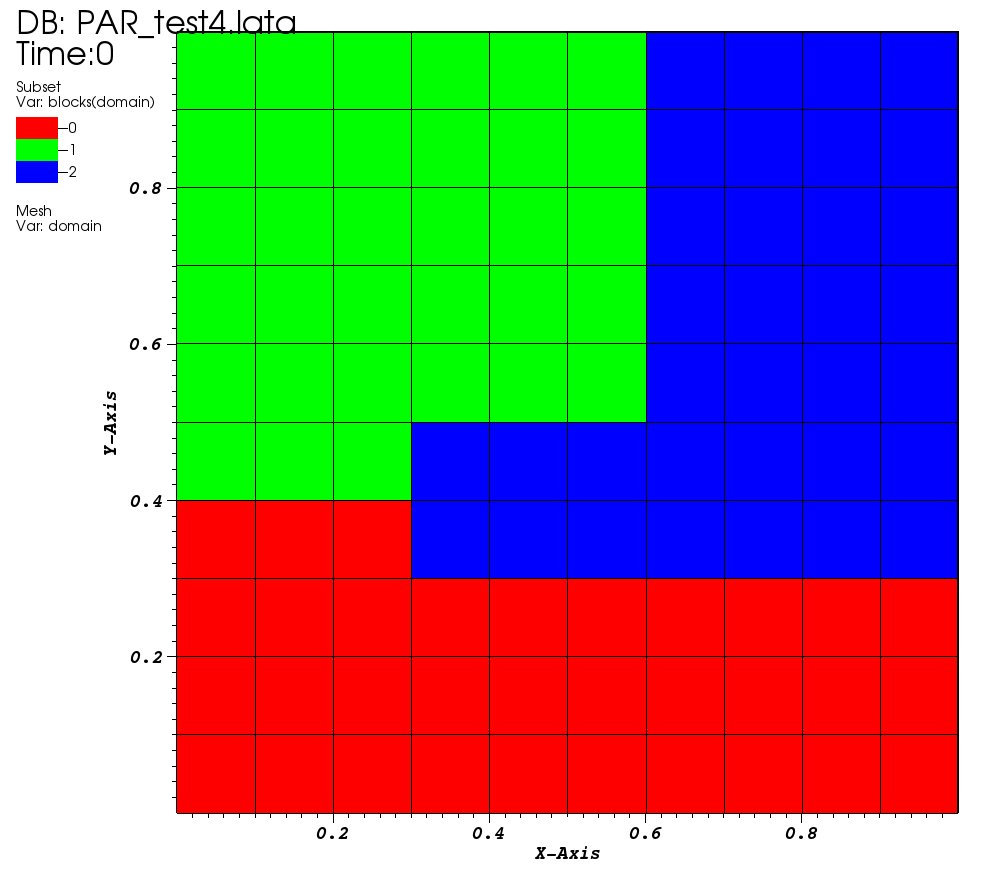
\includegraphics[width=0.45\textwidth]{partition_metis.jpeg} & & 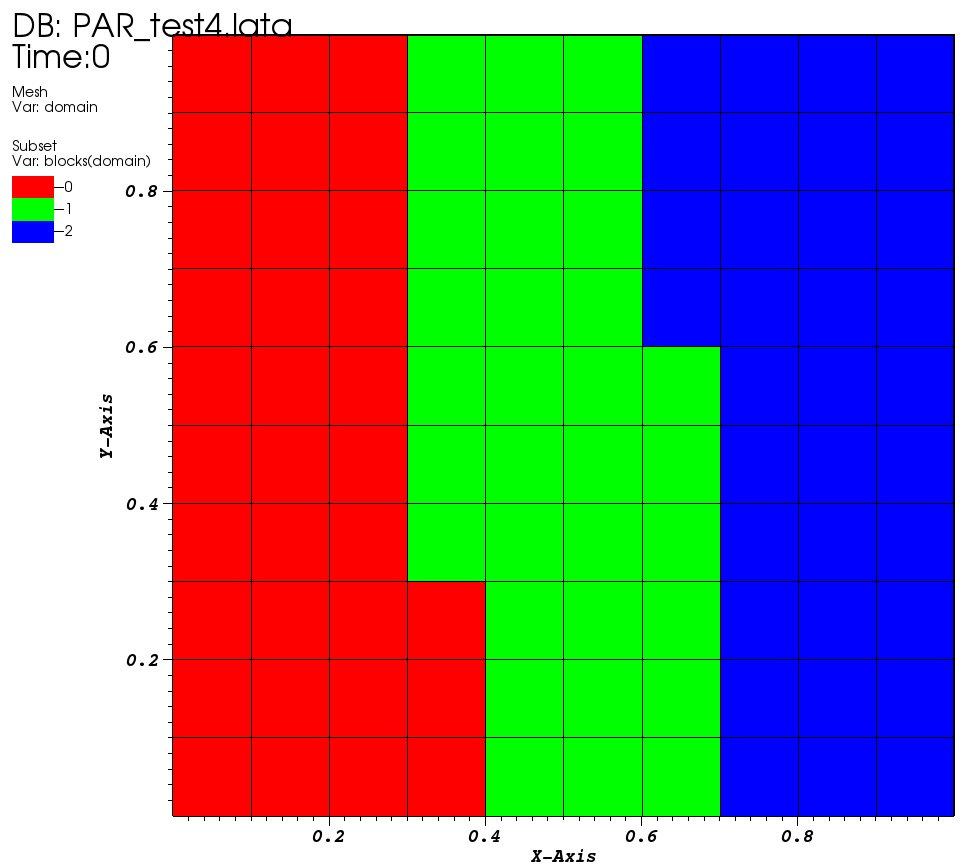
\includegraphics[width=0.45\textwidth]{partition_tranche.jpeg}\tabularnewline
METIS & & Tranche\tabularnewline
\end{tabular}
\par\end{centering}
\caption{Partitioning tools}
\label{partitioning}
\end{figure}

You can see the documentation of \href{\REFERENCEMANUAL\#partition}{this part in the \trustref Reference Manual}.



%%%%%%%%%%%%%%%%%%%%%%%%%%%%%%%%%%%%%%%%%%%%%%%%%
\subsection{Overlapping width value}
%%%%%%%%%%%%%%%%%%%%%%%%%%%%%%%%%%%%%%%%%%%%%%%%%
To make the partitioning, you will have to specify the \underline{overlapping width value}.
This value corresponds to the thickness of the virtual ghost zone (data known by one processor though not owned by it) i.e. the number of vertices or elements on the remote sub-domain known by the local sub-domain (cf Figure \ref{overlap}).

\begin{figure}[h!]
\begin{center}
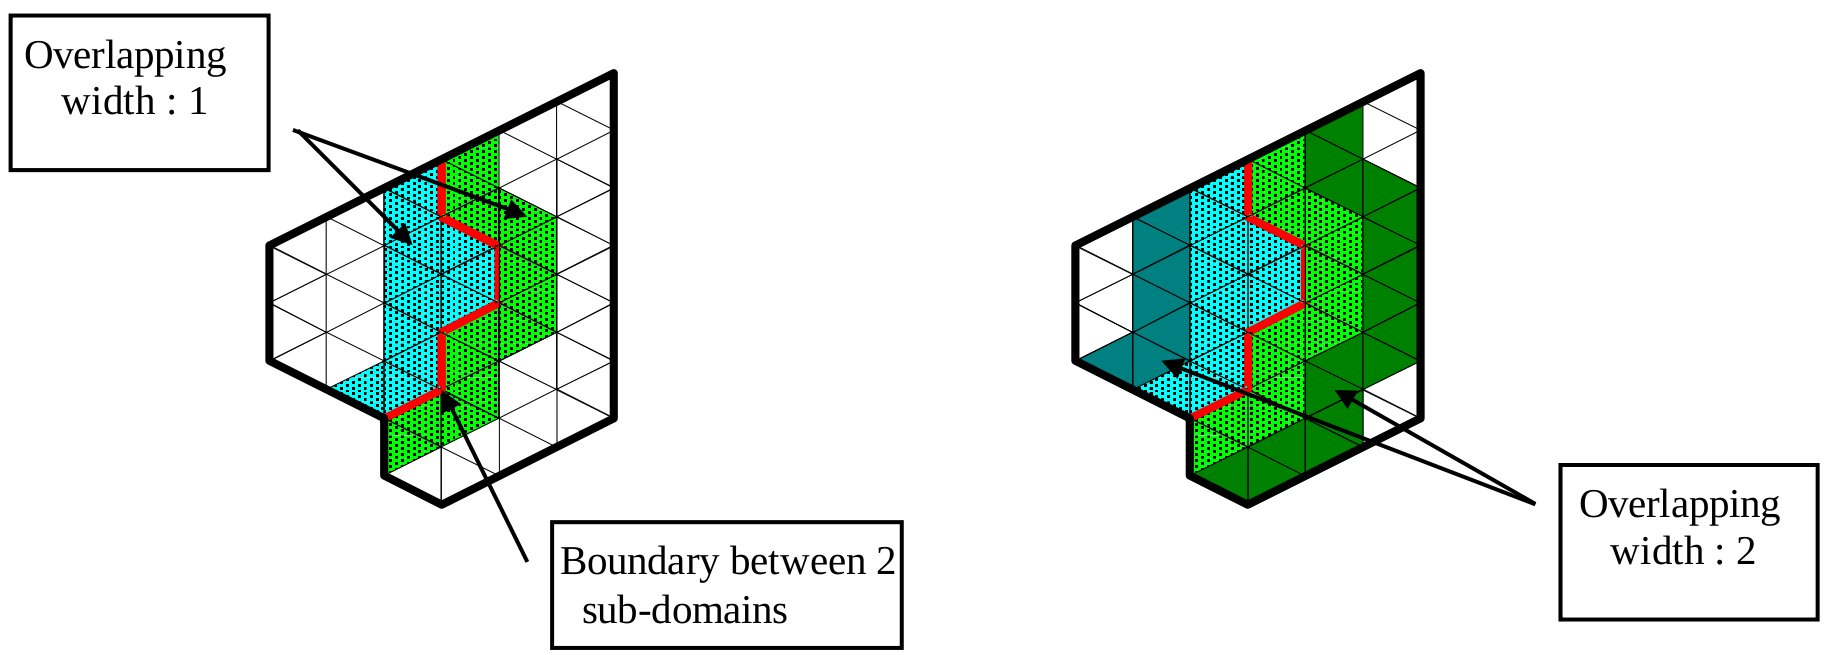
\includegraphics[width=0.96\textwidth]{overlap.jpeg}
\caption{Overlapping width}
\label{overlap}
\end{center}
\end{figure}

This value depends on the space discretization scheme orders:
\begin{itemize}
\item 1 if 1st or 2nd order,
\item 2 if 3rd or 4th order.
\end{itemize}

\Note that in general, you will use "2"!



%%%%%%%%%%%%%%%%%%%%%%%%%%%%%%%%%%%%%%%%%%%%%%%%%%%%%%%%%%%%%%%%%%%%%%%%
\section{Running a parallel calculation}
%%%%%%%%%%%%%%%%%%%%%%%%%%%%%%%%%%%%%%%%%%%%%%%%%%%%%%%%%%%%%%%%%%%%%%%%

%%%%%%%%%%%%%%%%%%%%%%%%%%%%%%%%%%%%%%%%%%%%%%%%%
\subsection{On a PC}
%%%%%%%%%%%%%%%%%%%%%%%%%%%%%%%%%%%%%%%%%%%%%%%%%
To launch the calculation, you have to run the calculation by the usual command completed by the number of processors needed:
\begin{verbatim}
> trust my_parallel_data_file procs_number
\end{verbatim}
and \textit{procs\_number} is the number of processors used. In fact it is the same as the number of sub-domains.\\

You can see the \trust \& \textbf{TrioCFD} user slides in the "Parallel calculation" section for more information and those two exercises of the \trust tutorial: \href{TRUST_tutorial.pdf\#exo_para_1}{exercise 1} and \href{TRUST_tutorial.pdf\#prm_para}{exercise 2}.

%%%%%%%%%%%%%%%%%%%%%%%%%%%%%%%%%%%%%%%%%%%%%%%%%
\subsection{On a cluster}
%%%%%%%%%%%%%%%%%%%%%%%%%%%%%%%%%%%%%%%%%%%%%%%%%
You must submit your job in a queue system.
For this, you must have a submission file.
\trust can create a submission file for you \textbf{on clusters on which the support team has done installations}.
To create this file, run:
\begin{verbatim}
> trust -create_sub_file my_parallel_data_file
\end{verbatim}

You obtain a file named \textbf{"sub\_file"}, you can open it and verify/change values(for example the name of the job, the name of the exe, ...).\\

Then you must submit you calculation with:
\begin{verbatim}
> sbatch sub_file
\end{verbatim}
or 
\begin{verbatim}
> ccc_msub sub_file
\end{verbatim}
following the queue system of the cluster.\\

%You can also run the same command as on a pc:
%\begin{verbatim}
%> trust my_parallel_data_file procs_number
%\end{verbatim}
%\trust will automatically submit your simulation.\\

You can see the \trust \& \textbf{TrioCFD} user slides in the "Parallel calculation" section for more information and \href{TRUST_tutorial.pdf\#exo_para_3}{this exercise of the \trust tutorial}.


%%%%%%%%%%%%%%%%%%%%%%%%%%%%%%%%%%%%%%%%%%%%%%%%%%%%%%%%%%%%%%%%%%%%%%%%
\section{Visualization}
%%%%%%%%%%%%%%%%%%%%%%%%%%%%%%%%%%%%%%%%%%%%%%%%%%%%%%%%%%%%%%%%%%%%%%%%
To visualize your probes, you can use the CurvePlot tool, with the command line:
\begin{verbatim}
> trust -evol my_parallel_data_file
\end{verbatim}
or use Gnuplot or any software which reads values in columns in a file.\\

There are three ways to visualize your parallel results with VisIt:
\begin{itemize}
\item HPCDrive on CCRT/TGCC clusters: opens a deported graphic session on dedicated nodes with more memory (on TGCC cluster: \href{https://visu-tgcc.ccc.cea.fr/HPCDrive/home}{HPCDrive}),
\item local mode: copy your results from the cluster to your local computer and open it with a local parallel version of VisIt with:
\begin{verbatim}
> visit -np 4 &
\end{verbatim}
\end{itemize}

You can have a look at the \trust \& \textbf{TrioCFD} user slides in the "Parallel calculation description" section.




%%%%%%%%%%%%%%%%%%%%%%%%%%%%%%%%%%%%%%%%%%%%%%%%%%%%%%%%%%%%%%%%%%%%%%%%
\section{Useful information}
%%%%%%%%%%%%%%%%%%%%%%%%%%%%%%%%%%%%%%%%%%%%%%%%%%%%%%%%%%%%%%%%%%%%%%%%
%%%%%%%%%%%%%%%%%%%%%%%%%%%%%%%%%%%%%%%%%%%%%%%%%
\subsection{Modify the mesh}
%%%%%%%%%%%%%%%%%%%%%%%%%%%%%%%%%%%%%%%%%%%%%%%%%
If you want to modify your mesh, you have two possibilities:
\begin{itemize} 
\item modify the \textit{my\_data\_file.data} file and run:
\begin{verbatim}
> trust -partition my_data_file [parts_number]
\end{verbatim}
Be carefull it will erase the \textit{SEQ\_my\_data\_file.data}, \textit{DEC\_my\_data\_file.data} and \\
\textit{PAR\_my\_data\_file.data} files and creates new ones.\\
Then it will run the new \textit{DEC\_my\_data\_file.data} file which gives your new \textit{DOM\_000n}\textbf{.Zones} files.

\item modify the meshing part of file \textit{DEC\_my\_data\_file.data} and run it with:
\begin{verbatim}
> trust DEC_my_data_file
\end{verbatim}
\end{itemize}

Then run the parallel calculation normally, on the new \textit{DOM\_000n}\textbf{.Zones} files.
\begin{verbatim}
> trust PAR_my_data_file procs_number
\end{verbatim}




%%%%%%%%%%%%%%%%%%%%%%%%%%%%%%%%%%%%%%%%%%%%%%%%%
\subsection{Modify calculation parameters}
%%%%%%%%%%%%%%%%%%%%%%%%%%%%%%%%%%%%%%%%%%%%%%%%%
If you want to modify the calculation parameters, you can modify:
\begin{itemize} 
\item the file \textit{my\_data\_file.data} and run:
\begin{verbatim}
> trust -partition data_file_name [parts_number]
\end{verbatim}
But it will erase the \textit{SEQ\_my\_data\_file.data}, \textit{DEC\_my\_data\_file.data} and \\
\textit{PAR\_my\_data\_file.data} files and create new ones.\\
Then it will run the new \textit{DEC\_my\_data\_file.data} file which gives your new \textit{DOM\_000n}\textbf{.Zones} files.\\
\Note that in that case, you don't need to re-create the mesh so you can use the second point below:
\item modify the \textit{PAR\_my\_data\_file.data} file \underline{without} running "trust -partition datafile" command line.
\end{itemize}
Then run the \textit{PAR\_my\_data\_file.data} file with:
\begin{verbatim}
> trust PAR_my_data_file procs_number
\end{verbatim}

\Note that if after a certain time, you want to reopen an old case and understand want you did in it without any doubts, you may create two files by hands:
\begin{itemize} 
\item one "BuildMeshes.data" file only for the mesh and the cut of the mesh, and
\item one "calculation.data" file for the parallel calculation. 
\end{itemize}
You will run it like:
\begin{verbatim}
> trust BuildMeshes
> trust calculation processors_number
\end{verbatim}

For this point, you can have a look at \href{TRUST_tutorial.pdf\#prm_para}{this exercise of the \trust tutorial}.






%%%%%%%%%%%%%%%%%%%%%%%%%%%%%%%%%%%%%%%%%%%%%%%%%%%%%%%%%%%%%%%%%%%%%%%%



%%%%%%%%%%%%%%%%%%%%%%%%%%%%%%%%%%%%%%%%%%%%%%%%%%%%%%%%%%%%%%%%%%%%%%%%%%
%%%
%%\chapter{Automatic validation form}
%%%
%%%%%%%%%%%%%%%%%%%%%%%%%%%%%%%%%%%%%%%%%%%%%%%%%%%%%%%%%%%%%%%%%%%%%%%%%%
%%%\input{chap8_prm.tex}
%%%%%%%%%%%%%%%%%%%%%%%%%%%%%%%%%%%%%%%%%%%%%%%%%%%%%%%%%%%%%%%%%%%%%%%%%%



\end{document}

'

\usepackage[unicode=true,pdfusetitle, bookmarks=true,bookmarksnumbered=false,bookmarksopen=false,
 breaklinks=false,pdfborder={0 0 1},backref=false,colorlinks=true,linkcolor=blue,pageanchor, urlcolor=darkblue]
 {hyperref}[2010/09/11]

\ifx \TRUSTV \undefined
\def\TRUSTVERSION{}
\else
\def\TRUSTVERSION{V\TRUSTV}
\fi
%\def \REFERENCEMANUAL {../../Outils/TRIOXDATA/XTriou/doc.pdf}
\def \REFERENCEMANUAL {TRUST_Reference_Manual.pdf}

\hypersetup{pdftitle={TRUST Generic Guide \TRUSTVERSION}, pdfauthor={Team TRUST} }

\usepackage[utf8]{inputenc}
\usepackage[T1]{fontenc}
\usepackage[top=2cm, bottom=2cm, left=2cm, right=2cm]{geometry}
\usepackage{babel}
\usepackage{alltt}
\usepackage{color}
\usepackage{longtable}
\usepackage{tikz}
\usepackage{xspace}
\usepackage{graphicx}
%\usepackage{times}

\setlength{\parindent}{0pt} % pas d'indentation

\definecolor{darkblue}{HTML}{3535B4}
\definecolor{LightSkyBlue}{HTML}{87CFFA}
\definecolor{DeepSkyBlue}{HTML}{00BFFF}
\definecolor{Greeen}{HTML}{439236}
\definecolor{mauve}{HTML}{874ad3}
\definecolor{vert}{HTML}{0ab351}
\definecolor{darkred}{HTML}{a31623}

\newenvironment{remark}{\textit{\underline{Remark:}}}{}
\newcommand{\trust}{\textbf{TRUST}\xspace}
\newcommand{\trustref}{Project\xspace}
\newcommand{\Note}{\textbf{\textcolor{darkred}{Note}}\xspace}


\begin{document}

\title{\vspace{2cm}\Huge \bfseries{TRUST Generic Guide \TRUSTVERSION}}
\author{
\vspace{2cm} % espace entre support team et ref manual
\LARGE \textbf{Support team: \href{mailto:triou@cea.fr}{triou@cea.fr}} \\
\vspace{1cm} % espace entre ref manual et la date
Link to: \LARGE \textbf{\href{run:\REFERENCEMANUAL}{\trustref Reference Manual}}\\
%%%%%%% Pour recuperer l'adresse d'un pdf par les variables d'environnement et makefile
%%%%%\ifx \BALTROOT \empty
%%%%%Link to: \LARGE \textbf{\href{run:\TRUSTROOTLATEX/Outils/TRIOXDATA/XTriou/doc.pdf}{\trustref Reference Manual}}\\
%%%%%\else
%%%%%Link to: \LARGE \textbf{\href{run:\BALTROOT/build/xdata/XTriou/doc.pdf}{\trustref Reference Manual}}\\
%%%%%\fi
}
%\date{} % si on ne veut pas la date

\maketitle
\tableofcontents{}
\newpage


%%%%%%%%%%%%%%%%%%%%%%%%%%%%%%%%%%%%%%%%%%%%%%%%%%%%%%%%%%%%%%%%%%%%%%%%
%
\chapter{Introduction}
%
%%%%%%%%%%%%%%%%%%%%%%%%%%%%%%%%%%%%%%%%%%%%%%%%%%%%%%%%%%%%%%%%%%%%%%%%
This document constitutes the generic guide for \textbf{TRUST software} and its \textbf{Baltik projects}.\\

\trust is a thermohydraulic software package for CFD simulations for incompressible monophasic flow.\\

You can create new project based on \trust plateform. Theses projects are named \textbf{"BALTIK"} projects.\\

The currently available modules include a VDF calculation module "Finite Difference Volume", a VEF calculation module "Finite Element Volume" and a PolyMAC module "series of Marker-and-Cell (MAC) schemes that can handle any type of mesh (non-conform, non-orthogonal, poly-hedral types, ...)". For further details, you can see https://cea-trust-platform.github.io/classes/discretizations/ \\

The VDF and VEF validated modules are designed to process the 2D or 3D flow of Newtonian, incompressible, weakly expandable fluids the density of which is a function of a local temperature and concentration values (Boussinesq approximation).



%%%%%%%%%%%%%%%%%%%%%%%%%%%%%%%%%%%%%%%%%%%%%%%%%%%%%%%%%%%%%%%
\section{Before TRUST: a modular software named Trio\_U}
%%%%%%%%%%%%%%%%%%%%%%%%%%%%%%%%%%%%%%%%%%%%%%%%%%%%%%%%%%%%%%%

\trust was born from the cutting in two pieces of \textbf{Trio\_U} software.
\textbf{Trio\_U} was a software brick based on the \textbf{Kernel} brick (which contains the equations, space discretizations, numerical schemes, parallelism...) and used by other CEA applications (cf Figure \ref{TrioU}).

\begin{figure}[h!]
\begin{center}
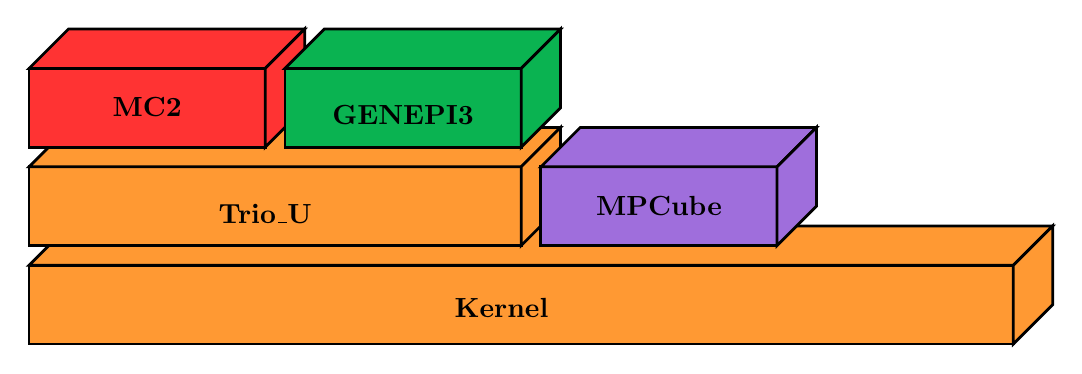
\begin{tikzpicture}[scale=2, line width=1pt]
% box Kernel
\coordinate (A) at (0,0) ;
\coordinate (B) at (6.25,0) ;
\coordinate (C) at (6.25,0.5) ;
\coordinate (D) at (0,0.5) ;
\coordinate (E) at (0.25,0.75) ;
\coordinate (F) at (6.5,0.75) ;
\coordinate (G) at (6.5,0.25) ;
\draw[black,fill=orange!80] (A) -- (B) -- (C) -- (D) -- cycle ;
\draw[black,fill=orange!80] (D) -- (C) -- (F) -- (E) -- cycle ;
\draw[black,fill=orange!80] (B) -- (C) -- (F) -- (G) -- cycle ;
\draw (3,0.1) node[above]{\textbf{Kernel}} ;
%% box Trio_U
\begin{scope}
\coordinate (A1) at (0,0.625) ;
\coordinate (B1) at (3.125,0.625) ;
\coordinate (C1) at (3.125,1.125) ;
\coordinate (D1) at (0,1.125) ;
\coordinate (E1) at (0.25,1.375) ;
\coordinate (F1) at (3.375,1.375) ;
\coordinate (G1) at (3.375,0.875) ;
\draw[black,fill=orange!80] (A1) -- (B1) -- (C1) -- (D1) -- cycle ;
\draw[black,fill=orange!80] (D1) -- (C1) -- (F1) -- (E1) -- cycle ;
\draw[black,fill=orange!80] (B1) -- (C1) -- (F1) -- (G1) -- cycle ;
\draw (1.5,0.7) node[above]{\textbf{Trio\_U}} ;
\end{scope}
% box MPCube
\begin{scope}[xshift=3.25 cm]
\coordinate (A1) at (0,0.625) ;
\coordinate (B1) at (1.5,0.625) ;
\coordinate (C1) at (1.5,1.125) ;
\coordinate (D1) at (0,1.125) ;
\coordinate (E1) at (0.25,1.375) ;
\coordinate (F1) at (1.75,1.375) ;
\coordinate (G1) at (1.75,0.875) ;
\draw[black,fill=mauve!80] (A1) -- (B1) -- (C1) -- (D1) -- cycle ;
\draw[black,fill=mauve!80] (D1) -- (C1) -- (F1) -- (E1) -- cycle ;
\draw[black,fill=mauve!80] (B1) -- (C1) -- (F1) -- (G1) -- cycle ;
\draw (0.75,0.75) node[above]{\textbf{MPCube}} ;
\end{scope}
%% box MC2
\begin{scope}[xshift=0 cm, yshift=0.625 cm]
\coordinate (A1) at (0,0.625) ;
\coordinate (B1) at (1.5,0.625) ;
\coordinate (C1) at (1.5,1.125) ;
\coordinate (D1) at (0,1.125) ;
\coordinate (E1) at (0.25,1.375) ;
\coordinate (F1) at (1.75,1.375) ;
\coordinate (G1) at (1.75,0.875) ;
\draw[black,fill=red!80] (A1) -- (B1) -- (C1) -- (D1) -- cycle ;
\draw[black,fill=red!80] (D1) -- (C1) -- (F1) -- (E1) -- cycle ;
\draw[black,fill=red!80] (B1) -- (C1) -- (F1) -- (G1) -- cycle ;
\draw (0.75,0.75) node[above]{\textbf{MC2}} ;
\end{scope}
% box GENEPI3
\begin{scope}[xshift=1.625 cm, yshift=0.625 cm]
\coordinate (A1) at (0,0.625) ;
\coordinate (B1) at (1.5,0.625) ;
\coordinate (C1) at (1.5,1.125) ;
\coordinate (D1) at (0,1.125) ;
\coordinate (E1) at (0.25,1.375) ;
\coordinate (F1) at (1.75,1.375) ;
\coordinate (G1) at (1.75,0.875) ;
\draw[black,fill=vert] (A1) -- (B1) -- (C1) -- (D1) -- cycle ;
\draw[black,fill=vert] (D1) -- (C1) -- (F1) -- (E1) -- cycle ;
\draw[black,fill=vert] (B1) -- (C1) -- (F1) -- (G1) -- cycle ;
\draw (0.75,0.7) node[above]{\textbf{GENEPI3}} ;
\end{scope}
\end{tikzpicture}
\caption{Trio\_U: brick software}
\label{TrioU}
\end{center}
\end{figure}

We could create new projects based on Kernel brick or \textbf{Trio\_U} brick. 
Theses projects were named \textbf{"BALTIK"} projects: "\textbf{B}uild an \textbf{A}pplication \textbf{L}inked to \textbf{T}r\textbf{I}o\_U \textbf{K}ernel".\\

In 2015, \textbf{Trio\_U} was divided in two parts: \trust and \textbf{TrioCFD}.
\begin{itemize}
\item \trust is a new platform, its name means: "\textbf{TR}io\_\textbf{U} \textbf{S}oftware for \textbf{T}hermohydraulics",
\item \textbf{TrioCFD} is a BALTIK project based on \trust, which contains the following models: FT, Radiation, LES, zoom...
\end{itemize}

Here is the structure of \trust platform (cf Figure \ref{TRUST}):

\begin{figure}[h!]
\begin{center}
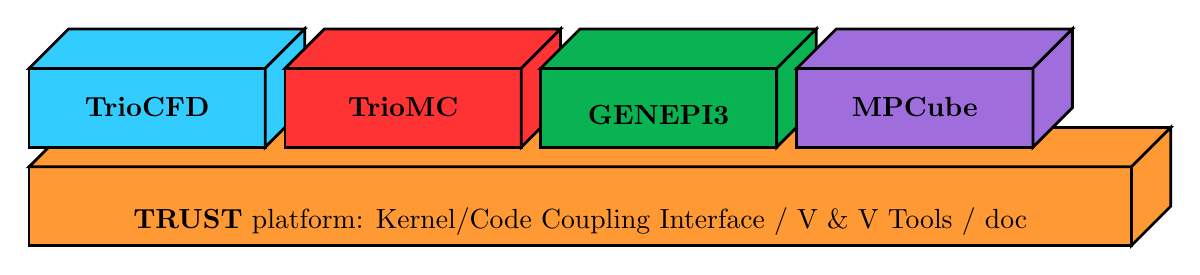
\begin{tikzpicture}[scale=2, line width=1pt]
% box TRUST
\coordinate (A) at (0,0) ;
\coordinate (B) at (7,0) ;
\coordinate (C) at (7,0.5) ;
\coordinate (D) at (0,0.5) ;
\coordinate (E) at (0.25,0.75) ;
\coordinate (F) at (7.25,0.75) ;
\coordinate (G) at (7.25,0.25) ;
\draw[black,fill=orange!80] (A) -- (B) -- (C) -- (D) -- cycle ;
\draw[black,fill=orange!80] (D) -- (C) -- (F) -- (E) -- cycle ;
\draw[black,fill=orange!80] (B) -- (C) -- (F) -- (G) -- cycle ;
\draw (3.5,0) node[above]{\trust platform: Kernel/Code Coupling Interface / V \& V Tools / doc} ;
%% box TrioCFD
\begin{scope}
\coordinate (A1) at (0,0.625) ;
\coordinate (B1) at (1.5,0.625) ;
\coordinate (C1) at (1.5,1.125) ;
\coordinate (D1) at (0,1.125) ;
\coordinate (E1) at (0.25,1.375) ;
\coordinate (F1) at (1.75,1.375) ;
\coordinate (G1) at (1.75,0.875) ;
\draw[black,fill=DeepSkyBlue!80] (A1) -- (B1) -- (C1) -- (D1) -- cycle ;
\draw[black,fill=DeepSkyBlue!80] (D1) -- (C1) -- (F1) -- (E1) -- cycle ;
\draw[black,fill=DeepSkyBlue!80] (B1) -- (C1) -- (F1) -- (G1) -- cycle ;
\draw (0.75,0.75) node[above]{\textbf{TrioCFD}} ;
\end{scope}
% box TrioMC
\begin{scope}[xshift=1.625 cm]
\coordinate (A1) at (0,0.625) ;
\coordinate (B1) at (1.5,0.625) ;
\coordinate (C1) at (1.5,1.125) ;
\coordinate (D1) at (0,1.125) ;
\coordinate (E1) at (0.25,1.375) ;
\coordinate (F1) at (1.75,1.375) ;
\coordinate (G1) at (1.75,0.875) ;
\draw[black,fill=red!80] (A1) -- (B1) -- (C1) -- (D1) -- cycle ;
\draw[black,fill=red!80] (D1) -- (C1) -- (F1) -- (E1) -- cycle ;
\draw[black,fill=red!80] (B1) -- (C1) -- (F1) -- (G1) -- cycle ;
\draw (0.75,0.75) node[above]{\textbf{TrioMC}} ;
\end{scope}
% box GENEPI3
\begin{scope}[xshift=3.248 cm]
\coordinate (A1) at (0,0.625) ;
\coordinate (B1) at (1.5,0.625) ;
\coordinate (C1) at (1.5,1.125) ;
\coordinate (D1) at (0,1.125) ;
\coordinate (E1) at (0.25,1.375) ;
\coordinate (F1) at (1.75,1.375) ;
\coordinate (G1) at (1.75,0.875) ;
\draw[black,fill=vert] (A1) -- (B1) -- (C1) -- (D1) -- cycle ;
\draw[black,fill=vert] (D1) -- (C1) -- (F1) -- (E1) -- cycle ;
\draw[black,fill=vert] (B1) -- (C1) -- (F1) -- (G1) -- cycle ;
\draw (0.75,0.7) node[above]{\textbf{GENEPI3}} ;
\end{scope}
%% box MPCube
\begin{scope}[xshift=4.875 cm]
\coordinate (A1) at (0,0.625) ;
\coordinate (B1) at (1.5,0.625) ;
\coordinate (C1) at (1.5,1.125) ;
\coordinate (D1) at (0,1.125) ;
\coordinate (E1) at (0.25,1.375) ;
\coordinate (F1) at (1.75,1.375) ;
\coordinate (G1) at (1.75,0.875) ;
\draw[black,fill=mauve!80] (A1) -- (B1) -- (C1) -- (D1) -- cycle ;
\draw[black,fill=mauve!80] (D1) -- (C1) -- (F1) -- (E1) -- cycle ;
\draw[black,fill=mauve!80] (B1) -- (C1) -- (F1) -- (G1) -- cycle ;
\draw (0.75,0.75) node[above]{\textbf{MPCube}} ;
\end{scope}
\end{tikzpicture}
\caption{TRUST platform \& its BALTIKs}
\label{TRUST}
\end{center}
\end{figure}

\Note that: \textbf{Trio\_U = TRUST + TrioCFD}.
%%%%%%%%%%%%%%%%%%%%%%%%%%%%%%%%%%%%%%%%%%%%%%%%%%%%%%%%%%%%%%%



%%%%%%%%%%%%%%%%%%%%%%%%%%%%%%%%%%%%%%%%%%%%%%%%%%%%%%%%%%%%%%%
\section{Short history}
%%%%%%%%%%%%%%%%%%%%%%%%%%%%%%%%%%%%%%%%%%%%%%%%%%%%%%%%%%%%%%%

\trust is now developed at the CEA/DES/ISAS/DM2S/SGLS service.
The project starts in 1994 and improved versions were built ever since:
\begin{itemize}
\item 1994: start of the project Trio\_U
\item 01/1997: v1.0 - VDF only
\item 06/1998: v1.1 - VEF version
\item 04/2000: v1.2 - parallel version
\item 07/2001: v1.3 - radiation model, in TrioCFD since v1.7
\item 11/2002: v1.4 - new LES turbulence models, in TrioCFD since v1.8
\item 02/2006: v1.5 - VDF/VEF Front Tracking, in TrioCFD since v1.7
\item 10/2009: v1.6 - data structure revamped
\item 06/2015: v1.7 - cut into \trust and \textbf{TrioCFD} + switch to open source
\item 11/2019: v1.8 - Turbulence features are moved from \trust to \textbf{TrioCFD} + PolyMAC discretization
\item 06/2022: v1.9 - Pb\_Multiphase in \trust + PolyMAC V2 discretization + Pb\_HEM in \textbf{TrioCFD}
\end{itemize}
%%%%%%%%%%%%%%%%%%%%%%%%%%%%%%%%%%%%%%%%%%%%%%%%%%%%%%%%%%%%%%%




%%%%%%%%%%%%%%%%%%%%%%%%%%%%%%%%%%%%%%%%%%%%%%%%%%%%%%%%%%%%%%%
\section{Data file}
%%%%%%%%%%%%%%%%%%%%%%%%%%%%%%%%%%%%%%%%%%%%%%%%%%%%%%%%%%%%%%%

To launch a calculation with \trust, you need to write a "data file" which is an input file for \trust and will contain all the information about your simulation.
Data files are written following some rules as shown below. But their language is not a programming language, users can't make loops or switch...\\

\Note that:
\begin{itemize}
\item lines between \textcolor{blue}{\# ... \#} and \textcolor{blue}{/* ... */} are comments,
\item in that document, words in \textbf{bold} are \trust keywords, you can highlight them in your file editor with the command line (details in section \ref{Run}):\\
\texttt{> trust -config gedit|vim|emacs}
\item braces "\{ \}" are elements that \trust reads and interprets, so don't forget them and \underline{put space} \underline{before and after them},
\item elements between bracket "[ ]" are optional.
\end{itemize}

%%%%%%%%%%%%%%%%%%%%%%%%%%%%%%%%%%%%%%%%%%%%%%%%%%%%
\subsection{Data file example: base blocks} \label{data}
%%%%%%%%%%%%%%%%%%%%%%%%%%%%%%%%%%%%%%%%%%%%%%%%%%%%
Here is the template of a basic sequential data file:\\

\fbox{ \begin{minipage}[c]{1\textwidth}
\begin{alltt}
\textcolor{blue}{\# Dimension 2D or 3D \#}

{\bf{Dimension}} 2
\end{alltt}
\end{minipage}}
\vspace{0.1cm}



\fbox{ \begin{minipage}[c]{1\textwidth}
\begin{alltt}
\textcolor{blue}{\# Problem definition \#}

{\bf{Pb\_hydraulique}} \textit{my\_problem}
\end{alltt}
\end{minipage}}
\vspace{0.1cm}



\fbox{ \begin{minipage}[c]{1\textwidth}
\begin{alltt}
\textcolor{blue}{\# Domain definition \#}

{\bf{Domaine}} \textit{my\_domain}
\end{alltt}
\end{minipage}}
\vspace{0.1cm}



\fbox{ \begin{minipage}[c]{1\textwidth}
\begin{alltt}
\textcolor{blue}{\# Mesh \#}

{\bf{Read\_file}} \textit{my\_mesh.geo} ;
\end{alltt}
\end{minipage}}
\vspace{0.1cm}



\fbox{ \begin{minipage}[c]{1\textwidth}
\begin{alltt} 
\textcolor{blue}{\# For parallel calculation only! \#}

\textcolor{blue}{\# For the first run: partitioning step \#}

\textcolor{blue}{{\bf{Partition}} \textit{my\_domain}}

\textcolor{blue}{\{}

\textcolor{blue}{\hspace{1cm}    {\bf{Partition\_tool}} \textit{partitioner\_name} \{ \textit{option1 option2 ...} \}}

\textcolor{blue}{\hspace{1cm}    {\bf{Larg\_joint}} \textit{2}}

\textcolor{blue}{\hspace{1cm}    {\bf{zones\_name}} \textit{DOM}}

\textcolor{blue}{\hspace{1cm}    ...}

\textcolor{blue}{\}}

\textcolor{blue}{{\bf{End}}}
\end{alltt}
\end{minipage}}
\vspace{0.1cm}



\fbox{ \begin{minipage}[c]{1\textwidth}
\begin{alltt} 
\textcolor{blue}{\# For parallel calculation only! \#}

\textcolor{blue}{\# For the second run: read of the sub-domains \#}

\textcolor{blue}{\# {\bf{Scatter}} \textit{DOM}{\bf{.Zones}} \textit{my\_domain} \#}
\end{alltt}
\end{minipage}}
\vspace{0.1cm}



\fbox{ \begin{minipage}[c]{1\textwidth}
\begin{alltt}
\textcolor{blue}{\# Discretization on hexa or tetra mesh \#}

{\bf{VDF}} \textit{my\_discretization}
\end{alltt}
\end{minipage}}
\vspace{0.1cm}



\fbox{ \begin{minipage}[c]{1\textwidth}
\begin{alltt}
\textcolor{blue}{\# Time scheme explicit or implicit \#}

{\bf{Scheme\_euler\_explicit}} \textit{my\_scheme}

{\bf{Read}} \textit{my\_scheme}

\{

\hspace{1cm}        \textcolor{blue}{\# Initial time \#}

\hspace{1cm}        \textcolor{blue}{\# Time step \#}

\hspace{1cm}        \textcolor{blue}{\# Output criteria \#}

\hspace{1cm}        \textcolor{blue}{\# Stop Criteria \#}

\}
\end{alltt}
\end{minipage}}
\vspace{0.1cm}



\fbox{ \begin{minipage}[c]{1\textwidth}
\begin{alltt}
\textcolor{blue}{\# Physical characteristics of medium \#}

{\bf{Fluide\_Incompressible}} \textit{my\_medium}

{\bf{Read}} \textit{my\_medium}

\{

\hspace{1cm}        ...

\}
\end{alltt}
\end{minipage}}
\vspace{0.1cm}



\fbox{ \begin{minipage}[c]{1\textwidth}
\begin{alltt}
\textcolor{blue}{\# Gravity vector definition \#}

{\bf{Uniform\_field}} \textit{my\_gravity}

{\bf{Read}} \textit{my\_gravity 2 0 -9.81}

\end{alltt}
\end{minipage}}
\vspace{0.1cm}



\fbox{ \begin{minipage}[c]{1\textwidth}
\begin{alltt}

\textcolor{blue}{\# Association between the different objects \#}

{\bf{Associate}} \textit{my\_problem my\_domain}

{\bf{Associate}} \textit{my\_problem my\_scheme}

{\bf{Associate}} \textit{my\_problem my\_medium}

{\bf{Associate}} \textit{my\_medium my\_gravity}
\end{alltt}
\end{minipage}}
\vspace{0.1cm}



\fbox{ \begin{minipage}[c]{1\textwidth}
\begin{alltt}
\textcolor{blue}{\# Discretization of the problem \#}

{\bf{Discretize}} \textit{my\_problem my\_discretization}
\end{alltt}
\end{minipage}}
\vspace{0.1cm}



\fbox{ \begin{minipage}[c]{1\textwidth}
\begin{alltt}
\textcolor{blue}{\# New domains for post-treatment \#}

\textcolor{blue}{\# By default each boundary condition of the domain is already extrated }

\textcolor{blue}{\hspace{0.2cm} with such name "my\_dom"\_boundaries\_"my\_BC" \#}

{\bf{Domaine}} \textit{plane}

{\bf{extraire\_surface}} 

\{

\hspace{1cm}        {\bf{domaine}} \textit{plane}

\hspace{1cm}        {\bf{probleme}} \textit{my\_probleme}

\hspace{1cm}        {\bf{condition\_elements}} (x>0.5)

\hspace{1cm}        {\bf{condition\_faces (1)}} 

\}
\end{alltt}
\end{minipage}}
\vspace{0.1cm}



\fbox{ \begin{minipage}[c]{1\textwidth}
\begin{alltt}
\textcolor{blue}{\# Problem description \#}

{\bf{Read}} \textit{my\_problem}

\{
\end{alltt}
\end{minipage}}
\vspace{0.1cm}



\fbox{ \begin{minipage}[c]{1\textwidth}
\begin{alltt}
\hspace{1cm}        \textcolor{blue}{\# hydraulic problem \#}

\hspace{1cm}        {\bf{Navier\_Stokes\_standard}}

\hspace{1cm}        \{

\hspace{2cm}                \textcolor{blue}{\# Choice of the pressure matrix solver \#}

\hspace{2cm}                {\bf{Solveur\_Pression}} \textit{solver} \{ ... \}

\hspace{2cm}                \textcolor{blue}{\# Diffusion operator \#}

\hspace{2cm}                {\bf{Diffusion}} \{ ... \}

\hspace{2cm}                \textcolor{blue}{\# Convection operator \#}

\hspace{2cm}                {\bf{Convection}} \{ ... \}

\hspace{2cm}                \textcolor{blue}{\# Sources \#}

\hspace{2cm}                {\bf{Sources}} \{ ... \}

\hspace{2cm}                \textcolor{blue}{\# Initial conditions \#}

\hspace{2cm}                {\bf{Initial\_conditions}} \{ ... \}

\hspace{2cm}                \textcolor{blue}{\# Boundary conditions \#}

\hspace{2cm}                {\bf{Boundary\_conditions}} \{ ... \}

\hspace{1cm}        \}
    \end{alltt}
\end{minipage}}
\vspace{0.1cm}



\fbox{ \begin{minipage}[c]{1\textwidth}
\begin{alltt}
\hspace{1cm}        \textcolor{blue}{\# Post\_processing description \#}

\hspace{1cm}        \textcolor{blue}{/* To know domains that can be treated directly, search in .err }

\hspace{1.6cm}       \textcolor{blue}{    output file: "Creating a surface domain named" */}

\hspace{1cm}        \textcolor{blue}{/* To know fields  that can be treated directly, search in .err }

\hspace{1.6cm}      \textcolor{blue}{     output file: "Reading of fields to be postprocessed" */}

\hspace{1cm}        {\bf{Post\_processing}}

\hspace{1cm}        \{

\hspace{2cm}                \textcolor{blue}{\# Definition of new fields \#}

\hspace{2cm}                {\bf{Definition\_Champs}} \{ ... \}


\hspace{2cm}                \textcolor{blue}{\# Probes \#}

\hspace{2cm}                {\bf{Probes}} \{ ... \}


\hspace{2cm}                \textcolor{blue}{\# Fields \#}

\hspace{2cm}                \textcolor{blue}{\# format default value: lml \#}

\hspace{2cm}                \textcolor{blue}{\# select 'lata' for VisIt tool or 'MED' for Salom\'e \#}

\hspace{2cm}                {\bf{format lata}}

\hspace{2cm}                {\bf{fields dt\_post}} 1. \{ ... \}


\hspace{2cm}                \textcolor{blue}{\# Statistical fields \#}

\hspace{2cm}                {\bf{Statistiques dt\_post}} 1. \{ ... \}

\hspace{1cm}        \} 
\end{alltt}
\end{minipage}}
\vspace{0.1cm}



\fbox{ \begin{minipage}[c]{1\textwidth}
\begin{alltt}
    \textcolor{blue}{\# Saving and restarting process \#}

    [{\bf{sauvegarde binaire}} \textit{datafile}{\bf{.sauv}}]

    [{\bf{resume\_last\_time binaire}} \textit{datafile}{\bf{.sauv}}]
\end{alltt}
\end{minipage}}
\vspace{0.1cm}


\fbox{ \begin{minipage}[c]{1\textwidth}
\begin{alltt}
\textcolor{blue}{\# End of the problem description block \#}

\}
\end{alltt}
\end{minipage}}
\vspace{0.1cm}



\fbox{ \begin{minipage}[c]{1\textwidth}
\begin{alltt}
\textcolor{blue}{\# The problem is solved with \#}

{\bf{Solve}} \textit{my\_problem}
\end{alltt}
\end{minipage}}
\vspace{0.1cm}



\fbox{ \begin{minipage}[c]{1\textwidth}
\begin{alltt}
\textcolor{blue}{\# Not necessary keyword to finish \#}

{\bf{End}}
\end{alltt}
\end{minipage}}


%%%%%%%%%%%%%%%%%%%%%%%%%%%%%%%%%%%%%%%%%%%%%%%%%%%%



%%%%%%%%%%%%%%%%%%%%%%%%%%%%%%%%%%%%%%%%%%%%%%%%%%%%
\subsection{Basic rules}
%%%%%%%%%%%%%%%%%%%%%%%%%%%%%%%%%%%%%%%%%%%%%%%%%%%%
There is no line concept in \trust.\\

Data files uses \underline{blocks}. They may be defined using the braces:\\
    \begin{center}
    \fbox{ \begin{minipage}[c]{0.5\textwidth}
    \begin{alltt}
    \{

    \hspace{1cm}    a block

    \}
    \end{alltt}
    \end{minipage}}
    \end{center}
\bigskip{}


%%%%%%%%%%%%%%%%%%%%%%%%%%%%%%%%%%%%%%%%%%%%%%%%%%%%



%%%%%%%%%%%%%%%%%%%%%%%%%%%%%%%%%%%%%%%%%%%%%%%%%%%%
\subsection{Objects notion}
%%%%%%%%%%%%%%%%%%%%%%%%%%%%%%%%%%%%%%%%%%%%%%%%%%%%
\textbf{Objects} are created in the data set as follows:
    \begin{center}
    \fbox{ \begin{minipage}[c]{0.5\textwidth}
    \begin{alltt}
        {\textit{ Type identificateur}}
    \end{alltt}
    \end{minipage}}
    \end{center}

\begin{itemize}
\item \textit{Type}: must be a type of object recognised by \trust, correspond to the C++ classes. The list of recognised types is given in the file hierarchie.dump.
\item \textit{identificateur}: the identifier of the object type \textit{Type} created, correspond to an instancy of the C++ class \textit{Type}. \trust exits in error if the identifier has already been used.
\end{itemize}

There are several object types. Physical objects, for example:

\begin{itemize}
%\item A block object (keyword \textbf{Pave}) is defined by its origin and dimensions (keyword \textbf{origine (origin)} and \textbf{longueurs (length)}). Discretization is given by the \textbf{nombre\_de\_noeuds (node number)} in each direction.
\item A \textbf{Fluide\_incompressible} (incompressible\_Fluid) object. This type of object is defined by its physical characteristics (its dynamic viscosity $\mu$ (keyword \textbf{mu}), its density $\rho$ (keyword \textbf{rho}), etc...),
\item A \textbf{Domaine}.
\end{itemize}

More abstract object types also exist:

\begin{itemize}
\item A \textbf{VDF}, \textbf{VEF} or \textbf{PolyMAC} according to the discretization type,
\item A \textbf{Scheme\_euler\_explicit} to indicate the time scheme type, here it's a first-order explicit Euler scheme,
\item A \textbf{Solveur\_pression} to denote the pressure system solver type,
\item A \textbf{Uniform\_field} to define, for example, the gravity field.
\end{itemize}
%%%%%%%%%%%%%%%%%%%%%%%%%%%%%%%%%%%%%%%%%%%%%%%%%%%%



%%%%%%%%%%%%%%%%%%%%%%%%%%%%%%%%%%%%%%%%%%%%%%%%%%%%
\subsection{Interpretor notion}
%%%%%%%%%%%%%%%%%%%%%%%%%%%%%%%%%%%%%%%%%%%%%%%%%%%%
\textbf{Interprete } (interpretor) type objects are then used to handle the created objects with the following syntax:
    \begin{center}
    \fbox{ \begin{minipage}[c]{0.5\textwidth}
    \begin{alltt}
        {\bf{\textit{Type\_interprete}}} \textit{argument}
    \end{alltt}
    \end{minipage}}
    \end{center}

\begin{itemize}
\item \textit{Type\_interprete}: any type derived from the \textbf{Interprete} (Interpretor) type recognised by \trust. In this manual, they are written in \textbf{bold}. You can highlight them in your file editor with the command (details in section \ref{Run}):\\
\texttt{> trust -config nedit|vim|emacs}
\item \textit{argument}: an argument may comprise one or several object identifiers and/or one or several data blocks.
\end{itemize}

Interpretors allow some operations to be carried out on objects.\\

Currently available general interpretors include \textbf{Read}, \textbf{Read\_file}, \textbf{Ecrire} (Write), \textbf{Ecrire\_fichier} (Write\_file), \textbf{Associate}.
%%%%%%%%%%%%%%%%%%%%%%%%%%%%%%%%%%%%%%%%%%%%%%%%%%%%



%%%%%%%%%%%%%%%%%%%%%%%%%%%%%%%%%%%%%%%%%%%%%%%%%%%%
\subsection{Example}
%%%%%%%%%%%%%%%%%%%%%%%%%%%%%%%%%%%%%%%%%%%%%%%%%%%%
%\begin{itemize}
%\item A data set to write Ok on screen:
A data set to write Ok on screen:
    \begin{center}
    \fbox{ \begin{minipage}[c]{0.9\textwidth}
    \begin{alltt}
    {\bf{Nom}} a\_name    \hspace{0.5cm}       \textcolor{blue}{\# Creation of an object type. Name identifier a\_name \#}

    {\bf{Read}} a\_name Ok        \textcolor{blue}{\# Allocates the string "Ok" to a\_name \#}

    {\bf{Ecrire}} a\_name     \hspace{0.2cm}     \textcolor{blue}{\# Write a\_name on screen \#}
    \end{alltt}
    \end{minipage}}
    \end{center}

%%%\item An incorrect data set:
%%%    \begin{center}
%%%    \fbox{ \begin{minipage}[c]{0.5\textwidth}
%%%    \begin{alltt}
%%%    {\bf{Domaine}} truc

%%%    ...

%%%    {\bf{Probleme}} truc   \textcolor{blue}{\# TRUST exits in error \#}
%%%    \end{alltt}
%%%    \end{minipage}}
%%%    \end{center}

%%%A possible correction:
%%%    \begin{center}
%%%    \fbox{ \begin{minipage}[c]{0.9\textwidth}
%%%    \begin{alltt}
%%%    \{

%%%    {\bf{Domaine}} truc

%%%    \}   \hspace{2.6cm}   \textcolor{blue}{\# The domain truc is destroyed \#}

%%%    {\bf{Probleme}} truc  \textcolor{blue}{\# this is correct because truc is not used any more \#}
%%%    \end{alltt}
%%%    \end{minipage}}
%%%    \end{center}


%\item One data set nesting another:
%    \begin{center}
%    \fbox{ \begin{minipage}[c]{0.9\textwidth}
%    \begin{alltt}
%    {\bf{Read\_file}} fichier\_inclus ; 

%    \textcolor{blue}{\# you should use {\bf{export}} in the fichier\_inclus to export identifiers \#}
%    \end{alltt}
%    \end{minipage}}
%    \end{center}

%example of the fichier\_inclus file: 
%    \begin{center}
%    \fbox{ \begin{minipage}[c]{0.9\textwidth}
%    \begin{alltt}
%    {\bf{Dimension}} 2

%    {\bf{export Domaine}} dom

%    {\bf{export Probleme\_hydraulique}} pb
%    \end{alltt}
%    \end{minipage}}
%    \end{center}
%\end{itemize}
%%%%%%%%%%%%%%%%%%%%%%%%%%%%%%%%%%%%%%%%%%%%%%%%%%%%



%%%%%%%%%%%%%%%%%%%%%%%%%%%%%%%%%%%%%%%%%%%%%%%%%%%%
\subsection{Important remarks}
%%%%%%%%%%%%%%%%%%%%%%%%%%%%%%%%%%%%%%%%%%%%%%%%%%%%
\begin{enumerate}
\item To insert \underline{comments} in the data set, use \textcolor{blue}{\# .. \#} (or \textcolor{blue}{/* ... */}), the character \textcolor{blue}{\#} must always be enclosed by blanks.
\item The comma separates items in a list (a comma must be enclosed with spaces or a new line).
\item Interpretor keywords are recognised indiscriminately whether they are written in lower and/or upper case.
\item \textbf{On the contrary, object names (identifiers) are recognised differently if they are written in upper or lower case.}
\item In the following description, items (keywords or values) enclosed by [ and ] are \underline{optional}.
\end{enumerate}
%%%%%%%%%%%%%%%%%%%%%%%%%%%%%%%%%%%%%%%%%%%%%%%%%%%%



%%%%%%%%%%%%%%%%%%%%%%%%%%%%%%%%%%%%%%%%%%%%%%%%%%%%%%%%%%%%%%%
\section{Running a data file}\label{Run}
%%%%%%%%%%%%%%%%%%%%%%%%%%%%%%%%%%%%%%%%%%%%%%%%%%%%%%%%%%%%%%%

To use \trust, your shell must be "bash". So ensure you are in the right shell:
\begin{verbatim}
> echo $0
/bin/bash
\end{verbatim}

To run your data file, you must initialize the TRUST environment using the following command:
\begin{verbatim}
> source $my_path_to_TRUST_installation/env_TRUST.sh
TRUST vX.Y.Z support : trust@cea.fr
Loading personal configuration /$path_to_my_home_directory/.perso_TRUST.env
\end{verbatim}


%%%%%%%%%%%%%%%%%%%%%%%%%%%%%%%%%%%%%%%%%%%%%%%%%%%%%%%%%%%%%%%
\subsection{Sequential calculation}
%%%%%%%%%%%%%%%%%%%%%%%%%%%%%%%%%%%%%%%%%%%%%%%%%%%%%%%%%%%%%%%
You can run your sequential calculation:
\begin{verbatim}
> cd $my_test_directory
> trust [-evol] my_data_file
\end{verbatim}

where "trust" command call the "trust" script.
You can have the list of its options with:
\begin{verbatim}
> trust -help
\end{verbatim}
or
\begin{verbatim}
> trust -h
\end{verbatim}

Here is a panel of available options:
\begin{verbatim}
Usage: trust [option] datafile [nb_cpus] [1>file.out] [2>file.err]
Where option may be:
-help|-h                      : List options.
-baltik [baltik_name]         : Instanciate an empty Baltik project.
-index                        : Access to the TRUST ressource index.
-doc                          : Access to the TRUST manual (Generic Guide).
-html                         : Access to the doxygen documentation.
-config nedit|vim|emacs|gedit : Configure nedit or vim or emacs or gedit with TRUST keywords.
-edit                         : Edit datafile.
-xcheck                       : Check the datafile's keywords with xdata.
-xdata                        : Check and run the datafile's keywords with xdata.
-partition                    : Partition the mesh to prepare a parallel calculation (Creation of the .Zones files).
-mesh                         : Visualize the mesh(es) contained in the data file.
-eclipse-trust                : Generate Eclipse configuration files to import TRUST sources.
-eclipse-baltik               : Generate Eclipse configuration files to import BALTIK sources (TRUST project should have been configured under Eclipse).
-probes                       : Monitor the TRUST calculation only.
-evol                         : Monitor the TRUST calculation (GUI).
-prm                          : Write a prm file (deprecated).
-jupyter                      : Create basic jupyter notebook file.
-clean                        : Clean the current directory from all the generated files by TRUST.
-search keywords              : Know the list of test cases from the data bases which contain keywords.
-copy                         : Copy the test case datafile from the TRUST database under the present directory.
-check|-ctest all|testcase|list            : Check|ctest the non regression of all the test cases or a single test case or a list of tests cases specified in a file.
-check|-ctest function|class|class::method : Check|ctest the non regression of a list of tests cases covering a function, a class or a class method.
-gdb                          : Run under gdb debugger.
-valgrind                     : Run under valgrind.
-valgrind_strict              : Run under valgrind with no suppressions.
-callgrind                    : Run callgrind tool (profiling) from valgrind.
-massif                       : Run massif tool (heap profile) from valgrind.
-heaptrack                    : Run heaptrack (heap profile). Better than massif.
-advisor                      : Run advisor tool (vectorization).
-vtune                        : Run vtune tool (profiling).
-perf                         : Run perf tool (profiling).
-trace                        : Run traceanalyzer tool (MPI profiling).
-create_sub_file              : Create a submission file only.
-prod                         : Create a submission file and submit the job on the main production class with exclusive resource.
-bigmem                       : Create a submission file and submit the job on the big memory production class.
-queue queue                  : Create a submission file with the specified queue and submit the job.
-c ncpus                      : Use ncpus CPUs allocated per task for a parallel calculation.
datafile -help_trust          : Print options of TRUST_EXECUTABLE [CASE[.data]] [options].
-convert_data datafile        : Convert a data file to the new 1.9.1 syntax (milieu, interfaces, read_med and champ_fonc_med).

\end{verbatim}

%-monitor                : Run and monitor the progress of the TRUST calculation.
%-probes                 : Monitor the TRUST calculation only.
%-bigmem                 : Create a submission file and submit the job on the big 
%                          memory production class. 
%-queue queue            : Create a submission file with the specified queue and 
%                          submit the job. 
%-c ncpus                : Use ncpus CPUs allocated per task for a parallel 
%                          calculation. 


\newpage
%%%%%%%%%%%%%%%%%%%%%%%%%%%%%%%%%%%%%%%%%%%%%%%%%%%%%%%%%%%%%%%
\subsection{Parallel calculation}
%%%%%%%%%%%%%%%%%%%%%%%%%%%%%%%%%%%%%%%%%%%%%%%%%%%%%%%%%%%%%%%
To run a parallel calculation, you must do two runs:
\begin{itemize}
\item the first one, to partition and create your 'n' sub-domains (two methods: "By hand" method below and "Assisted" method cf parts \ref{decjdd} \& \ref{makePARdata}),
\item the second one, to read your 'n' sub-domains and run the calculation on 'n' processors.
\end{itemize}
\vspace{0.5cm}

We will explain here how to do such work:
\begin{itemize}
\item \textbf{\textcolor{darkblue}{Partitioning: "By hand" method}}\\
You have to make two data files:
\begin{itemize}
\item \textit{BuildMeshes.data} and 
\item \textit{Calculation.data}.
\end{itemize}

The \textit{BuildMeshes.data} file only contains the same information as the 
begining of the sequential data file and partitioning information.
This file will create the sub-domains (cf .Zones files).


\begin{center}
\fbox{ \begin{minipage}[c]{0.8\textwidth}
\begin{center}
\textit{BuildMeshes.data}
\end{center}
\end{minipage}}
\fbox{ \begin{minipage}[c]{0.8\textwidth}
\begin{alltt} 
{\bf{Dimension}} 2

{\bf{Domaine}} \textit{my\_domain}


\textcolor{blue}{\# BEGIN MESH \#}

{\bf{Read\_file}} \textit{my\_mesh.geo} ;

\textcolor{blue}{\# END MESH \#}


\textcolor{blue}{\# BEGIN PARTITION \#}

{\bf{Partition}} \textit{my\_domain}

\{

\hspace{1cm}    {\bf{Partition\_tool}} \textit{partitioner\_name} \{ \textit{option1 option2 ...} \}

\hspace{1cm}    {\bf{Larg\_joint}} \textit{2}

\hspace{1cm}    {\bf{zones\_name}} \textit{DOM}

\hspace{1cm}    ...

\}

{\bf{End}}

\textcolor{blue}{\# END PARTITION \#}
\end{alltt}
\end{minipage}}
\end{center}

Run the \textit{BuildMeshes.data} with \trust:
\begin{verbatim}
> trust BuildMeshes
\end{verbatim}

You may have obtained files named \textit{DOM\_000n}\textbf{.Zones} which contains the 'n' sub-domains.\\



\item \textbf{\textcolor{darkblue}{Read the sub-domains}}\\
%To see your sub-domains, you can run:
%\begin{alltt} 
%> trust -mesh Calculation
%\end{alltt}

The \textit{Calculation.data} file contains the domain definition, the block which will read the sub-domains and the problem definition (as in sequential calculation).
\begin{center}
\fbox{ \begin{minipage}[c]{0.8\textwidth}
\begin{center}
\textit{Calculation.data}
\end{center}
\end{minipage}}
\fbox{ \begin{minipage}[c]{0.8\textwidth}
\begin{alltt} 
{\bf{Dimension}} 2


{\bf{Domaine}} \textit{my\_domain}

{\bf{Pb\_Hydraulique}} \textit{my\_problem}

\textcolor{blue}{\# BEGIN SCATTER \#}

{\bf{Scatter}} \textit{DOM}{\bf{.Zones}} \textit{my\_domain}

\textcolor{blue}{\# END SCATTER \#}


{\bf{VDF}} \textit{my\_discretization}


{\bf{Scheme\_euler\_explicit}} \textit{my\_scheme}

{\bf{Read}} \textit{my\_scheme} \{ ... \}


{\bf{Associate}} \textit{my\_problem my\_domain}

{\bf{Associate}} \textit{my\_problem my\_scheme}


{\bf{Discretize}} \textit{my\_problem my\_discretization}


{\bf{Read}} \textit{my\_problem} \{ 

\hspace{1cm} {\bf{Fluide\_Incompressible}} \{ ... \}

\hspace{1cm} ... 

\}


{\bf{Solve}} \textit{my\_problem}


{\bf{End}}
\end{alltt}
\end{minipage}}
\end{center}

Run the \textit{Calculation.data} file with \trust:
\begin{verbatim}
> trust Calculation procs_number
\end{verbatim}


This will read your \textit{DOM\_000n}\textbf{.Zones} files. You can see the documentation of the \textbf{"scatter"} keyword in \href{\REFERENCEMANUAL\#scatter}{this part of the \trustref Reference Manual}.\\
\end{itemize}


For more information, you can see this \href{TRUST_tutorial.pdf\#exo_para_1}{exercise in the \trust tutorial}.




%%%%%%%%%%%%%%%%%%%%%%%%%%%%%%%%%%%%%%%%%%%%%%%%%%%%%%%%%%%%%%%
\section{Visualization}
%%%%%%%%%%%%%%%%%%%%%%%%%%%%%%%%%%%%%%%%%%%%%%%%%%%%%%%%%%%%%%%
To learn how to use the "\textbf{-evol}" option, you can see the first exercise of the \trust tutorial: \href{TRUST_tutorial.pdf\#exo1}{Flow around an obstacle}.



%%%%%%%%%%%%%%%%%%%%%%%%%%%%%%%%%%%%%%%%%%%%%%%%%%%%%%%%%%%%%%%%%%%%%%%%



%%%%%%%%%%%%%%%%%%%%%%%%%%%%%%%%%%%%%%%%%%%%%%%%%%%%%%%%%%%%%%%%%%%%%%%%
%
\chapter{Important references}
%
%%%%%%%%%%%%%%%%%%%%%%%%%%%%%%%%%%%%%%%%%%%%%%%%%%%%%%%%%%%%%%%%%%%%%%%%
For details and practices, see:
\begin{itemize}
\item \href{TRUST_tutorial.pdf}{the \trust tutorial},
\item \href{TRUST_and_TrioCFD_presentation.pdf}{the \trust \& \textbf{TrioCFD} presentation}: presentation slides of \trust and \textbf{TrioCFD},
\item \href{User_Manual_TRUST.pdf}{the \trust user manual}: full documentation of \trust,
\end{itemize}

Other references:
\begin{itemize}
\item Methodology for incompressible single phase flow (Models\_Equations\_TRUST.pdf),
\item Trio\_U code validation data base \& best practice guidelines (Best\_Practice\_TRUST.pdf),
\item Organisation of TrioCFD validation data base (HowTo\_Validation.pdf),
\item \trust development presentation (Developer\_TRUST\_presentation.pdf).
\end{itemize}

%%%%%%%%%%%%%%%%%%%%%%%%%%%%%%%%%%%%%%%%%%%%%%%%%%%%%%%%%%%%%%%%%%%%%%%%



%%%%%%%%%%%%%%%%%%%%%%%%%%%%%%%%%%%%%%%%%%%%%%%%%%%%%%%%%%%%%%%%%%%%%%%%
%
\chapter{Data setting}
%
%%%%%%%%%%%%%%%%%%%%%%%%%%%%%%%%%%%%%%%%%%%%%%%%%%%%%%%%%%%%%%%%%%%%%%%%
We will now explain how to fill a data file.
First you must specify some basic informations like the dimension of your domain, his name, the problem type...
To define the problem dimension, we use the following keyword:

    \begin{center}
    \fbox{ \begin{minipage}[c]{0.5\textwidth}
    \begin{alltt}
    {\bf{Dimension}}  \textit{2}  or {\bf{Dimension}}  \textit{3}
    \end{alltt}
    \end{minipage}}
    \end{center}


%%%%%%%%%%%%%%%%%%%%%%%%%%%%%%%%%%%%%%%%%%%%%%%%%%%%%%%%%%%%%%%
\section{Problems} \label{pbs}
%%%%%%%%%%%%%%%%%%%%%%%%%%%%%%%%%%%%%%%%%%%%%%%%%%%%%%%%%%%%%%%
You have to define the problem type that you wishes to solve.

    \begin{center}
    \fbox{ \begin{minipage}[c]{0.5\textwidth}
    \begin{alltt}
    {\bf{Pb\textit{\_type}}} \textit{my\_problem}
    \end{alltt}
    \end{minipage}}
    \end{center}

Here are some of the available problems types:
\begin{itemize}
%\item \textbf{Pb\_Hydraulique$\left[\mbox{\_Turbulent}\right]$}
%\item \textbf{Pb\_Thermohydraulique$\left[\mbox{\_Turbulent}\right]$}
%\item \textbf{Pb\_Hydraulique\_Concentration$\left[\mbox{\_Turbulent}\right]$}
\item for incompressible flow: \textbf{Pb\_$\left[\mbox{\textcolor{magenta}{Thermo}}\right]$hydraulique$\left[\mbox{\textcolor{darkblue}{\_Concentration}}\right]\hspace{-0.15cm}\left[\mbox{\textcolor{Greeen}{\_Turbulent}}\right]$},
\item for quasi-compressible flow: \textbf{Pb\_Thermohydraulique$\left[\mbox{\textcolor{Greeen}{\_Turbulent}}\right]$\_QC}, 
%\item for quasi-compressible flow:\\
%    \textbf{Pb\_Thermohydraulique$\left[\mbox{\textcolor{Greeen}{\_Turbulent}}\right]$\_QC$\left[\mbox{\textcolor{mauve}{\_fraction\_massique}}\right]$}, 
\item for solid: \textbf{Pb\_Conduction},
\item you can find all \href{\REFERENCEMANUAL\#Pbbase}{problem types} in the Reference Manual.
\end{itemize}


where:
\begin{itemize}
\item \textbf{hydraulique}: means that we will solve Navier Stokes equations without energy equation,
\item \textbf{\textcolor{magenta}{Thermo}}: means that we will solve Navier Stokes equations with energy equation,
\item \textbf{\textcolor{darkblue}{Concentration}}: that we will solve multiple constituent transportation equations,
\item \textbf{\textcolor{Greeen}{Turbulent}}: that we will simulate a turbulent flow and specify a turbulent model (RANS or LES),
\item \textbf{Conduction}: resolution of the heat equation,
\item \textbf{QC}: Navier Stokes equations with energy equation for quasi-compressible fluid under low Mach numbers,
%\item \textbf{\textcolor{mauve}{fraction\_massique}}: hydraulic and energy equations are solved and a list of passive scalar equations may be added.
\end{itemize}





%%%%%%%%%%%%%%%%%%%%%%%%%%%%%%%%%%%%%%%%%%%%%%%%%%%%%%%%%%%%%%%
\section{Domain definition}
%%%%%%%%%%%%%%%%%%%%%%%%%%%%%%%%%%%%%%%%%%%%%%%%%%%%%%%%%%%%%%%
To define the domain, you must name. This is done thanks to the following block:

    \begin{center}
    \fbox{ \begin{minipage}[c]{0.5\textwidth}
    \begin{alltt}
    {\bf{Domaine}}  \textit{my\_domain}
    \end{alltt}
    \end{minipage}}
    \end{center}

Then you must add your mesh to your simulation.




%%%%%%%%%%%%%%%%%%%%%%%%%%%%%%%%%%%%%%%%%%%%%%%%%%%%%%%%%%%%%%%
\section{Mesh} \label{Mesh}
%%%%%%%%%%%%%%%%%%%%%%%%%%%%%%%%%%%%%%%%%%%%%%%%%%%%%%%%%%%%%%%

Notice the presence of the tags:
\begin{alltt} 
\textcolor{blue}{\# BEGIN MESH \#}
...
\textcolor{blue}{\# END MESH \#}
\end{alltt}
in the data file of section \ref{data}.
This is necessary for parallel calculation (see section \ref{parallel}).

%%%%%%%%%%%%%%%%%%%%%%%%%%%%%%%%%%%%%%
\subsection{Allowed meshes}
%%%%%%%%%%%%%%%%%%%%%%%%%%%%%%%%%%%%%%
\trust allows:
\begin{itemize}
\item quadrangular or triangular undeformed meshing for 2D cases (Figure \ref{2D_mesh}),
\begin{figure}[h!]
\begin{center}

\begin{tikzpicture}[scale=2, line width=1pt]
\coordinate (A) at (0,0) ;
\coordinate (B) at (1.5,0) ;
\coordinate (C) at (1.5,1) ;
\coordinate (D) at (0,1) ;
\draw[black] (A) -- (B) -- (C) -- (D) -- cycle ;
\coordinate (E) at (3,0) ;
\coordinate (F) at (4.5,0) ;
\coordinate (G) at (3.75,1) ;
\draw[black] (E) -- (F) -- (G) -- cycle ;
\end{tikzpicture}
\caption{2D allowed elements}
\label{2D_mesh}
\end{center}
\end{figure}

\item hexahedral or tetrahedral undeformed meshing for 3D cases (Figure \ref{3D_mesh}).
\begin{figure}[h!]
\begin{center}
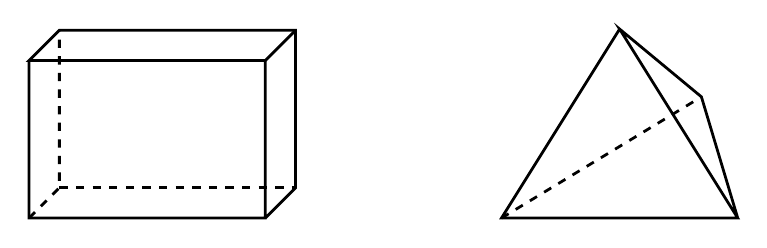
\begin{tikzpicture}[scale=2, line width=1pt]
\coordinate (A) at (0  ,0  ,0) ;
\coordinate (B) at (1.5,0  ,0) ;
\coordinate (C) at (1.5,1  ,0) ;
\coordinate (D) at (0  ,1  ,0) ;
\coordinate (E) at (0  ,0  ,-0.5) ;
\coordinate (F) at (1.5,0  ,-0.5) ;
\coordinate (G) at (1.5,1  ,-0.5) ;
\coordinate (H) at (0  ,1  ,-0.5) ;
\draw (D) -- (A) -- (B) -- (C) -- (D) -- (H) -- (G) -- (F) -- (B);
\draw (C) -- (G);
\draw [dashed] (A) -- (E) -- (H);
\draw [dashed] (E) -- (F);
\coordinate (I) at (3   ,0  ,0) ;
\coordinate (J) at (4.5 ,0  ,0) ;
\coordinate (K) at (3.75,1.2,0) ;
\coordinate (L) at (4   ,0.5,-0.7) ;
\draw[black] (K) -- (I) -- (J) -- (K) -- (L) -- (J) ;
\draw [dashed] (I) -- (L);
\end{tikzpicture}
\caption{3D allowed elements}
\label{3D_mesh}
\end{center}
\end{figure}
\end{itemize}

\textbf{Be carefull} non standard and hybrih meshing are not supported! (cf Figure \ref{hybr})

\begin{figure}[h!]
\begin{center}
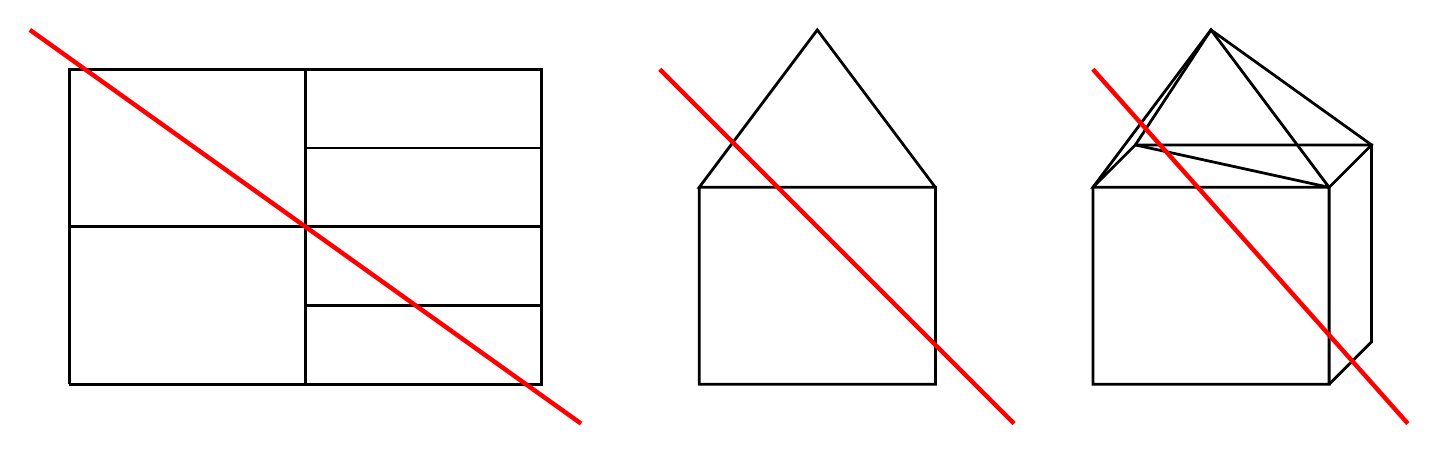
\begin{tikzpicture}[scale=2, line width=1pt]
\coordinate (A1) at (0,0) ;
\coordinate (A2) at (0,1) ;
\coordinate (A3) at (0,2) ;
\coordinate (B1) at (1.5,0  ) ;
\coordinate (B2) at (1.5,0.5) ;
\coordinate (B3) at (1.5,1  ) ;
\coordinate (B4) at (1.5,1.5) ;
\coordinate (B5) at (1.5,2  ) ;
\coordinate (C1) at (3,0  ) ;
\coordinate (C2) at (3,0.5) ;
\coordinate (C3) at (3,1  ) ;
\coordinate (C4) at (3,1.5) ;
\coordinate (C5) at (3,2  ) ;
\draw (A1) -- (C1) -- (C5) -- (A3) -- (A1);
\draw (A2) -- (C3);
\draw (B1) -- (B5);
\draw (B4) -- (C4);
\draw (B2) -- (C2);
\draw [ultra thick,red] (-0.25,2.25) -- (3.25,-0.25) ;

\coordinate (D1) at (4   ,0) ;
\coordinate (D2) at (5.5 ,0) ;
\coordinate (D3) at (5.5 ,1.25) ;
\coordinate (D4) at (4   ,1.25) ;
\coordinate (D5) at (4.75,2.25) ;
\draw (D4) -- (D1) -- (D2) -- (D3) -- (D4) -- (D5) -- (D3);
\draw [ultra thick,red] (3.75,2) -- (6,-0.25) ;

\coordinate (E1) at (6.5 ,0   ,0) ;
\coordinate (E2) at (8   ,0   ,0) ;
\coordinate (E3) at (8   ,1.25,0) ;
\coordinate (E4) at (6.5 ,1.25,0) ;
\coordinate (E5) at (7.25,2.25,0) ;
\coordinate (E6) at (8   ,0   ,-0.7) ;
\coordinate (E7) at (8   ,1.25,-0.7) ;
\coordinate (E8) at (6.5 ,1.25,-0.7) ;
\draw (E4) -- (E1) -- (E2) -- (E3) -- (E4) -- (E5) -- (E3);
\draw (E2) -- (E6) -- (E7) -- (E8) -- (E4);
\draw (E8) -- (E5) -- (E7) -- (E3) -- (E8);
\draw [ultra thick,red] (6.5,2) -- (8.5,-0.25) ;

\end{tikzpicture}
\caption{Prohibited meshes}
\label{hybr}
\end{center}
\end{figure}









%%%%%%%%%%%%%%%%%%%%%%%%%%%%%%%%%%%%%%
\subsection{Import mesh file}
%%%%%%%%%%%%%%%%%%%%%%%%%%%%%%%%%%%%%%
If your mesh was generated with an external tool like \href{http://www.salome-platform.org}{Salom\'e} (open source software), \href{http://resource.ansys.com/Products/Other+Products/ANSYS+ICEM+CFD}{ICEM} (commercial software), \href{http://gmsh.info/}{Gmsh} (open source software, included in \trust package) or \href{http://www-cast3m.cea.fr/}{Cast3M} (CEA software), then you must use one of the following keyword into your data file:

\begin{itemize}
\item \href{\REFERENCEMANUAL\#readmed}{\textbf{Read\_MED}} for a MED file from \href{http://www.salome-platform.org}{Salom\'e}, \href{http://gmsh.info/}{Gmsh},... ,
\item \href{\REFERENCEMANUAL\#readfile}{\textbf{Read\_File}} for a binary mesh file from \href{http://resource.ansys.com/Products/Other+Products/ANSYS+ICEM+CFD}{ICEM},
\item for another format, see the \href{\REFERENCEMANUAL\#read}{\trust Reference Manual}.
\end{itemize}

If you want to learn how to make a mesh with Salom\'e or Gmsh and read it with \trust, you can go to see the exercises of the \trust tutorial: \href{TRUST_tutorial.pdf\#salome}{here} for Salom\'e and \href{TRUST_tutorial.pdf\#gmsh}{here} for Gmsh.




%%%%%%%%%%%%%%%%%%%%%%%%%%%%%%%%%%%%%%
\subsection{Create quickly a mesh}
%%%%%%%%%%%%%%%%%%%%%%%%%%%%%%%%%%%%%%
Here is an example of a simple geometry (of non complex channel type) using the internal tool of \trust:
\begin{center}
\fbox{ \begin{minipage}[c]{0.9\textwidth}
\begin{alltt}
{\bf{Mailler}} \textit{my\_domain}

\{

\hspace{1cm}        \textcolor{blue}{/* Define the domain with one cavity */}

\hspace{1cm}        \textcolor{blue}{/* cavity 1m*2m with 5*22 cells */}

\hspace{1cm}        {\bf{Pave}} \textit{box}

\hspace{1cm}        \{

\hspace{2cm}            {\bf{Origine}} 0. 0.

\hspace{2cm}            {\bf{Longueurs}} 1 2

\hspace{2cm}            \textcolor{blue}{/* Cartesian grid */}

\hspace{2cm}            {\bf{Nombre\_de\_Noeuds}} 6 23

\hspace{2cm}            \textcolor{blue}{/* Uniform mesh */}

\hspace{2cm}            {\bf{Facteurs}} 1. 1.

\hspace{1cm}        \}

\hspace{1cm}        \{

\hspace{2cm}            \textcolor{blue}{/* Definition and names of boundary conditions */}

\hspace{2cm}            {\bf{bord}} \textit{Inlet}   \hspace{0.25cm} X = 0.  0. <= Y <= 2.

\hspace{2cm}            {\bf{bord}} \textit{Outlet}  \hspace{0.05cm} X = 1.  0. <= Y <= 2.

\hspace{2cm}            {\bf{bord}} \textit{Upper}   \hspace{0.25cm} Y = 2.  0. <= X <= 1.

\hspace{2cm}            {\bf{bord}} \textit{Lower}   \hspace{0.25cm} Y = 0.  0. <= X <= 1.

\hspace{1cm}        \}

\}
\end{alltt}
\end{minipage}}
\end{center}

To use this mesh in your data file, you just have to add the previous block in your data file or save it in a file named for example "\textit{my\_mesh.geo}" and add the line:\\
\begin{center}
\fbox{ \begin{minipage}[c]{0.5\textwidth}
\begin{alltt}
{\bf{Read\_file}} \textit{my\_mesh.geo} \textcolor{red}{{\bf{;}}}
\end{alltt}
\end{minipage}}
\end{center}

\underline{Do not forget the semi-colonn at the end of the line!}\\




%%%%%%%%%%%%%%%%%%%%%%%%%%%%%%%%%%%%%%
\subsection{Transform mesh within data file}
%%%%%%%%%%%%%%%%%%%%%%%%%%%%%%%%%%%%%%
You can also made transformations on your mesh after the \textbf{"Mailler"} or \textbf{"Read\_*"} command, using the following keywords:
\begin{itemize}
\item \href{\REFERENCEMANUAL\#triangulate}{\textbf{Trianguler}} to triangulate your 2D cells and create an unstructured mesh.
\item \href{\REFERENCEMANUAL\#tetraedriser}{\textbf{Tetraedriser}} to tetrahedralise 3D cells and create an unstructured mesh.
\item \href{\REFERENCEMANUAL\#raffineranisotrope}{\textbf{Raffiner\_anisotrope}}/\href{\REFERENCEMANUAL\#raffinerisotrope}{\textbf{Raffiner\_isotrope}} to triangulate/tetrahedralise elements of an untructured mesh.
\item \href{\REFERENCEMANUAL\#extrudebord}{\textbf{ExtrudeBord}} to generate an extruded mesh from a boundary of a tetrahedral or an hexahedral mesh. 
\Note that ExtrudeBord in VEF generates 3 or 14 tetrahedra from extruded prisms.
\item \href{\REFERENCEMANUAL\#regroupebord}{\textbf{RegroupeBord}} to build a new boundary with several boundaries of the domain.
\item \href{\REFERENCEMANUAL\#transformer}{\textbf{Transformer}} to transform the coordinates of the geometry.
\item for other commands, see the section \href{\REFERENCEMANUAL\#interprete}{interprete} of the \trust Reference Manual.
\end{itemize}

\Note that theses mesh modifications work on all mesh type (i.e. also for \textbf{*.geo} or \textbf{*.bin} or \textbf{*.med} files).



%%%%%%%%%%%%%%%%%%%%%%%%%%%%%%%%%%%%%%
\subsection{Test your mesh}
%%%%%%%%%%%%%%%%%%%%%%%%%%%%%%%%%%%%%%
The keyword \href{\REFERENCEMANUAL\#discretiserdomaine}{\textbf{Discretiser\_domaine}} is useful to discretize the domain (faces will be created) without defining a problem.
Indeed, you can create a minimal data file, post-process your mesh in lata format (for example) and visualize it with VisIt. \\

\Note that you must name all the boundaries!\\

Here is an example of this kind of data file:

\begin{center}
\fbox{ \begin{minipage}[c]{0.8\textwidth}
\begin{center}
\textbf{my\_data\_file.data}
\end{center}
\end{minipage}}
\fbox{ \begin{minipage}[c]{0.8\textwidth}
\begin{alltt}
{\bf{dimension 3}}

{\bf{Domaine}} \textit{my\_domain}

{\bf{Mailler}} \textit{my\_domain}

\{

\hspace{1cm}    {\bf{Pave}} \textit{box}

\hspace{1cm}    \{

\hspace{2cm}        {\bf{Origine}} 0. 0. 0.

\hspace{2cm}        {\bf{Longueurs}} 1 2 1

\hspace{2cm}        {\bf{Nombre\_de\_Noeuds}} 6 23 6

\hspace{2cm}        {\bf{Facteurs}} 1. 1. 1.

\hspace{1cm}    \}

\hspace{1cm}    \{

\hspace{2cm}        {\bf{bord}} \textit{Inlet}  \hspace{0.25cm} X = 0. 0. <= Y <= 2.  0. <= Z <= 1.

\hspace{2cm}        {\bf{bord}} \textit{Outlet} \hspace{0.05cm} X = 1.  0. <= Y <= 2.  0. <= Z <= 1.

\hspace{2cm}        {\bf{bord}} \textit{Upper}  \hspace{0.25cm} Y = 2.  0. <= X <= 1.  0. <= Z <= 1.

\hspace{2cm}        {\bf{bord}} \textit{Lower}  \hspace{0.25cm} Y = 0. 0. <= X <= 1.  0. <= Z <= 1.

\hspace{2cm}        {\bf{bord}} \textit{Front}  \hspace{0.25cm} Z = 0. 0. <= X <= 1.  0. <= Y <= 2.

\hspace{2cm}        {\bf{bord}} \textit{Back}   \hspace{0.45cm} Z = 1. 0. <= X <= 1.  0. <= Y <= 2.

\hspace{1cm}    \}

\}

{\bf{discretiser\_domaine}} \textit{my\_domain}

{\bf{postraiter\_domaine}} \{ {\bf{domaine}} \textit{my\_domain} {\bf{format lata}} \}

{\bf{End}}
    \end{alltt}
\end{minipage}}
\end{center}

To use it, launch in a bash terminal:
\begin{verbatim}
# if not already done
> source $my_path_to_TRUST_installation/env_TRUST.sh
# then
> trust my_data_file
> visit -o my_data_file.lata &
\end{verbatim}

To see how to use VisIt, go to see the first \trust tutorial exercise: \href{TRUST_tutorial.pdf\#exo1}{Obstacle}.\\

If you want to learn how to make a mesh with Salom\'e or Gmsh and read it with \trust, you can go to see the exercises of the \trust tutorial: \href{TRUST_tutorial.pdf\#salome}{here} for Salom\'e and \href{TRUST_tutorial.pdf\#gmsh}{here} for Gmsh.







%%%%%%%%%%%%%%%%%%%%%%%%%%%%%%%%%%%%%%%%%%%%%%%%%%%%%%%%%%%%%%%
\section{Discretization}
%%%%%%%%%%%%%%%%%%%%%%%%%%%%%%%%%%%%%%%%%%%%%%%%%%%%%%%%%%%%%%%
You have to specify the discretization type which can be \href{\REFERENCEMANUAL\#vdf}{\textbf{VDF}}, \href{\REFERENCEMANUAL\#ef}{\textbf{EF}} or \href{\REFERENCEMANUAL\#vefprep1b}{\textbf{VEFPreP1B}}.\\

In \textbf{VDF} discretization, the locations of the unknown are drawn in the Figure \ref{fig_VDF}.\\

\begin{figure}[h!]
\begin{center}
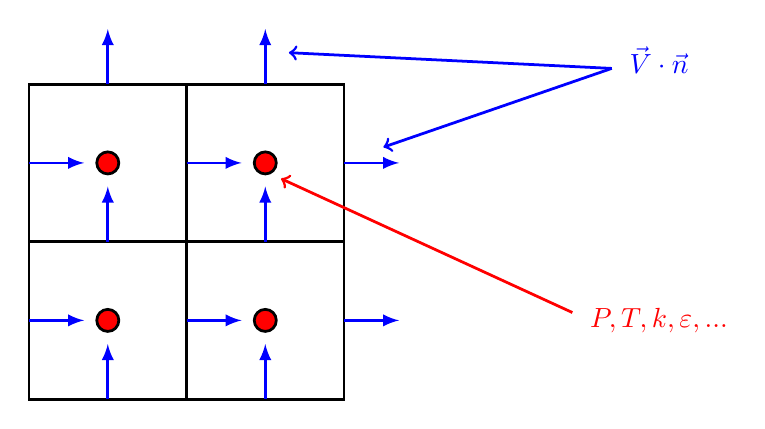
\begin{tikzpicture}[scale=2, line width=1pt]
\coordinate (A) at (0,0) ;
\coordinate (B) at (1,0) ;
\coordinate (C) at (2,0) ;
\coordinate (D) at (2,1) ;
\coordinate (E) at (2,2) ;
\coordinate (F) at (1,2) ;
\coordinate (G) at (0,2) ;
\coordinate (H) at (0,1) ;
\draw[black] (A) -- (C) -- (E) -- (G) -- cycle ;
\draw[black] (H) -- (D) ;
\draw[black] (F) -- (B) ;
\draw[black,fill=red] (0.5,0.5) circle (0.07);
\draw[black,fill=red] (1.5,0.5) circle (0.07);
\draw[black,fill=red] (0.5,1.5) circle (0.07);
\draw[black,fill=red] (1.5,1.5) circle (0.07);
\draw[blue] [->] [>=latex] (0.5,0) -- (0.5,0.35);
\draw[blue] [->] [>=latex] (0.5,1) -- (0.5,1.35);
\draw[blue] [->] [>=latex] (0.5,2) -- (0.5,2.35);
\draw[blue] [->] [>=latex] (1.5,0) -- (1.5,0.35);
\draw[blue] [->] [>=latex] (1.5,1) -- (1.5,1.35);
\draw[blue] [->] [>=latex] (1.5,2) -- (1.5,2.35);
\draw[blue] [->] [>=latex] (0,0.5) -- (0.35,0.5);
\draw[blue] [->] [>=latex] (1,0.5) -- (1.35,0.5);
\draw[blue] [->] [>=latex] (2,0.5) -- (2.35,0.5);
\draw[blue] [->] [>=latex] (0,1.5) -- (0.35,1.5);
\draw[blue] [->] [>=latex] (1,1.5) -- (1.35,1.5);
\draw[blue] [->] [>=latex] (2,1.5) -- (2.35,1.5);
\draw[blue] (4,2) node[above]{$\vec{V} \cdot \vec{n}$} ;
\draw[blue] [<-] (1.65,2.2) -- (3.7,2.1);
\draw[blue] [<-] (2.25,1.6) -- (3.7,2.1);
\draw[red] (4,0.5) node {$P, T, k, \varepsilon, ...$} ;
\draw[red] [<-] (1.6,1.4) -- (3.45,0.55);
\end{tikzpicture}
\caption{VDF unknown localisations}
\label{fig_VDF}
\end{center}
\end{figure}

For \textbf{VEFPreP1B}, the locations of the unknown are drawn in the Figure \ref{fig_VEF}.\\

\begin{figure}[h!]
\begin{center}
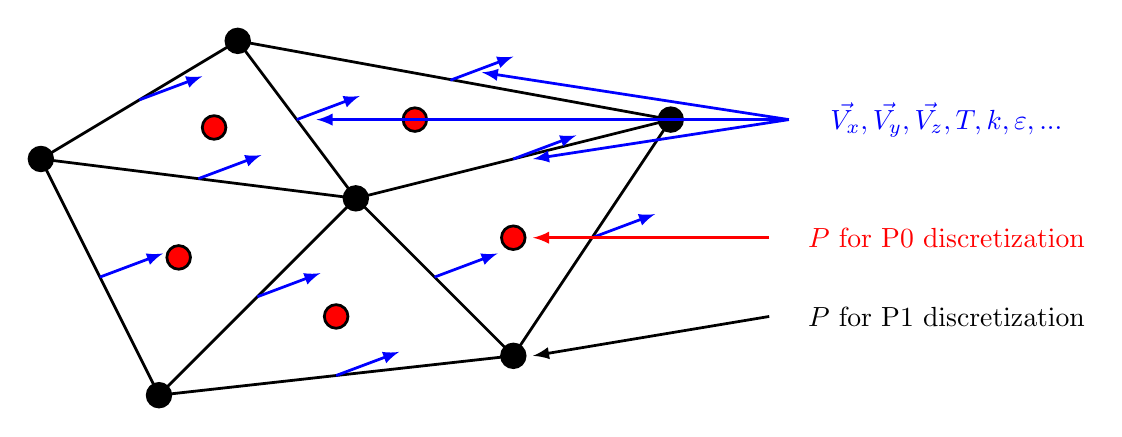
\begin{tikzpicture}[scale=1, line width=1pt]
\coordinate (A) at (1.5,0) ;
\coordinate (B) at (6,0.5) ;
\coordinate (C) at (8,3.5) ;
\coordinate (D) at (2.5,4.5) ;
\coordinate (E) at (0,3) ;
\coordinate (F) at (4,2.5) ;
\draw[black] (A) -- (B) -- (C) -- (D) -- (E) -- (A) -- (F) -- (B);
\draw[black] (C) -- (F) -- (D);
\draw[black] (E) -- (F);
\draw[black,fill=black] (A) circle (0.15);
\draw[black,fill=black] (B) circle (0.15);
\draw[black,fill=black] (C) circle (0.15);
\draw[black,fill=black] (D) circle (0.15);
\draw[black,fill=black] (E) circle (0.15);
\draw[black,fill=black] (F) circle (0.15);
\draw[black,fill=red] (3.75,1) circle (0.15);
\draw[black,fill=red] (6,2) circle (0.15);
\draw[black,fill=red] (4.75,3.5) circle (0.15);
\draw[black,fill=red] (2.2,3.4) circle (0.15);
\draw[black,fill=red] (1.75,1.75) circle (0.15);
\begin{scope}[xshift=5cm, yshift=1.5cm]
\draw[blue] [->] [>=latex] (0,0) -- (0.8,0.3);
\end{scope}
\begin{scope}[xshift=7cm, yshift=2cm]
\draw[blue] [->] [>=latex] (0,0) -- (0.8,0.3);
\end{scope}
\begin{scope}[xshift=5.2cm, yshift=4cm]
\draw[blue] [->] [>=latex] (0,0) -- (0.8,0.3);
\end{scope}
\begin{scope}[xshift=1.25cm, yshift=3.75cm]
\draw[blue] [->] [>=latex] (0,0) -- (0.8,0.3);
\end{scope}
\begin{scope}[xshift=0.75cm, yshift=1.5cm]
\draw[blue] [->] [>=latex] (0,0) -- (0.8,0.3);
\end{scope}
\begin{scope}[xshift=2.75cm, yshift=1.25cm]
\draw[blue] [->] [>=latex] (0,0) -- (0.8,0.3);
\end{scope}
\begin{scope}[xshift=3.75cm, yshift=0.25cm]
\draw[blue] [->] [>=latex] (0,0) -- (0.8,0.3);
\end{scope}
\begin{scope}[xshift=6cm, yshift=3cm]
\draw[blue] [->] [>=latex] (0,0) -- (0.8,0.3);
\end{scope}
\begin{scope}[xshift=3.25cm, yshift=3.5cm]
\draw[blue] [->] [>=latex] (0,0) -- (0.8,0.3);
\end{scope}
\begin{scope}[xshift=2cm, yshift=2.75cm]
\draw[blue] [->] [>=latex] (0,0) -- (0.8,0.3);
\end{scope}
\draw[blue] (11.5,3.5) node {$\vec{V_x}, \vec{V_y}, \vec{V_z}, T, k, \varepsilon, ...$} ;
\draw[blue] [->] [>=latex] (9.5,3.5) -- (5.6,4.1);
\draw[blue] [->] [>=latex] (9.5,3.5) -- (3.5,3.5);
\draw[blue] [->] [>=latex] (9.5,3.5) -- (6.25,3);
\draw[red] (11.5,2) node {$P$ for P0 discretization} ;
\draw[red] [->] [>=latex] (9.25,2) -- (6.25,2);
\draw[black] (11.5,1) node {$P$ for P1 discretization} ;
\draw[black] [->] [>=latex] (9.25,1) -- (6.25,0.5);
\end{tikzpicture}
\caption{VEF unknown localisations in 2D}
\label{fig_VEF}
\end{center}
\end{figure}

In 3D for the pressure, we can also use the P0+P1+Pa discretization for flow with a strong source term and a low velocity field.
In this case P0+P1 pressure gradient has trouble to match the source term so we use P0+P1+Pa discretization (cf Figure \ref{fig_VEF_pressure_loc}).

\begin{figure}[h!]
\begin{center}
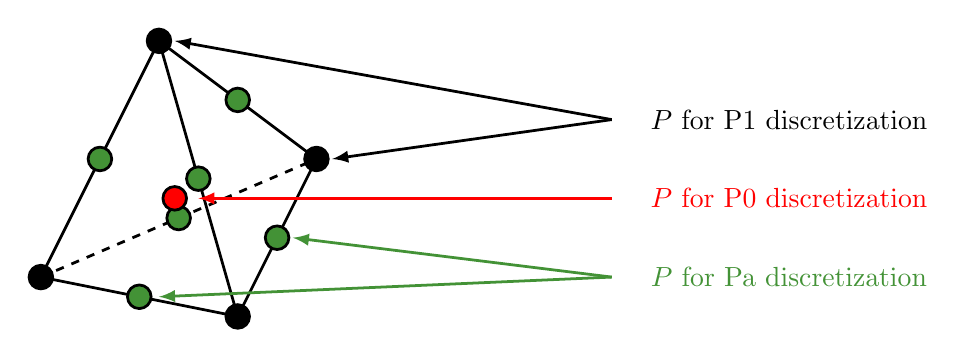
\begin{tikzpicture}[scale=1, line width=1pt]
\coordinate (A) at (0.5,1) ;
\coordinate (B) at (3,0.5) ;
\coordinate (C) at (4,2.5) ;
\coordinate (D) at (2,4) ;
\draw[black] (B) -- (C) -- (D) -- (A) -- (B) -- (D);
\draw[black,dashed] (A) -- (C);
\draw[black,fill=black] (A) circle (0.15);
\draw[black,fill=black] (B) circle (0.15);
\draw[black,fill=black] (C) circle (0.15);
\draw[black,fill=black] (D) circle (0.15);
\draw[black,fill=Greeen] (1.75,0.75) circle (0.15);
\draw[black,fill=Greeen] (3.5,1.5) circle (0.15);
\draw[black,fill=Greeen] (3,3.25) circle (0.15);
\draw[black,fill=Greeen] (1.25,2.5) circle (0.15);
\draw[black,fill=Greeen] (2.25,1.75) circle (0.15);
\draw[black,fill=Greeen] (2.5,2.25) circle (0.15);
\draw[black,fill=red] (2.2,2) circle (0.15);
\draw[black] (10,3) node {$P$ for P1 discretization} ;
\draw[black] [->] [>=latex] (7.75,3) -- (2.2,4);
\draw[black] [->] [>=latex] (7.75,3) -- (4.2,2.5);
\draw[red] (10,2) node {$P$ for P0 discretization} ;
\draw[red] [->] [>=latex] (7.75,2) -- (2.5,2);
\draw[Greeen] (10,1) node {$P$ for Pa discretization} ;
\draw[Greeen] [->] [>=latex] (7.75,1) -- (3.7,1.5);
\draw[Greeen] [->] [>=latex] (7.75,1) -- (2,0.75);
\end{tikzpicture}
\caption{VEF pressure localisation in 3D}
\label{fig_VEF_pressure_loc}
\end{center}
\end{figure}

To specify the wanted discretization, you have to add the following block to your data file:

    \begin{center}
    \fbox{ \begin{minipage}[c]{0.5\textwidth}
    \begin{alltt}
    \textit{{\bf{Discretization\_type}} my\_discretization}

    [{\bf{Read }} \textit{my\_discretization \{ ... \}}]
    \end{alltt}
    \end{minipage}}
    \end{center}

You can add parameters to your discretization with the optional keyword \href{\REFERENCEMANUAL\#read}{\textbf{Read}} (see \href{\REFERENCEMANUAL\#vefprep1b}{\textbf{VEFPreP1B discretization}}).

On the \href{http://www-trio-u.cea.fr/scripts/home/publigen/content/templates/show.asp?L=EN&P=55&vTicker=alleza&ITEMID=3}{TRUST website}, you can find information about:
\begin{itemize}
\item \textbf{VDF} discretization in the \href{http://www-trio-u.cea.fr/home/liblocal/docs/Theses/these_chatelain_2004.pdf}{PhD thesis of A. Chatelain},
\item \textbf{VEFPreP1B} discretization (Crouzet-Raviart elements) in the \href{http://www-trio-u.cea.fr/home/liblocal/docs/Theses/these_fortin_2006.pdf}{PhD thesis of T. Fortin} and \href{http://www-trio-u.cea.fr/home/liblocal/docs/Theses/These_Heib_2003.pdf}{PhD thesis of S. Heib}.
\end{itemize}


%%%%%%%%%%%%%%%%%%%%%%%%%%%%%%%%%%%%%%%%%%%%%%%%%%%%%%%%%%%%%%%
\section{Time schemes}
%%%%%%%%%%%%%%%%%%%%%%%%%%%%%%%%%%%%%%%%%%%%%%%%%%%%%%%%%%%%%%%
Now you can choose your time scheme to solve your problem. For this you must
specify the time scheme type wanted and give it a name. 
then you have to specify its parameters by filling the associated \textbf{"Read"} block.

    \begin{center}
    \fbox{ \begin{minipage}[c]{0.5\textwidth}
    \begin{alltt}
    {\bf{\textit{Scheme\_type}}} \textit{my\_time\_scheme}

    {\bf{Read}} \textit{my\_time\_scheme} \{ ... \}
    \end{alltt}
    \end{minipage}}
    \end{center}

%%%%%%%%%%%%%%%%%%%%%%%%%%%%%%%%%%%%%%
\subsection{Some available time schemes}
%%%%%%%%%%%%%%%%%%%%%%%%%%%%%%%%%%%%%%
%Here are some \href[page=DOCLINK_TIME SCHEMES]{\REFERENCEMANUAL}{available types of explicit schemes}:
Here are some available types of explicit schemes:
\begin{itemize}
\item \href{\REFERENCEMANUAL\#eulerscheme}{\textbf{Scheme\_Euler\_explicit}},
\item \href{\REFERENCEMANUAL\#schemaadamsbashforthorder2}{\textbf{Schema\_Adams\_Bashforth\_order\_2}},
%\item \textbf{Schema\_Adams\_Bashforth\_order\_3}
%\item \textbf{Runge\_Kutta\_Rationnel\_ordre\_2}
\item \href{\REFERENCEMANUAL\#rungekuttaordre3}{\textbf{Runge\_Kutta\_ordre\_3}},
%\item \textbf{Runge\_Kutta\_ordre\_4\_D3P}
%\item \textbf{Schema\_Predictor\_Corrector}
%\item \textbf{Sch\_CN\_iteratif}
%\item \textbf{Sch\_CN\_EX\_iteratif}
%\item \textbf{Schema\_Phase\_Field}
%\item \textbf{RK3\_FT}
\end{itemize}

%And also some \href[page=DOCLINK_TIME SCHEMES]{\REFERENCEMANUAL}{available types of implicit schemes}:
And also some available types of implicit schemes:
\begin{itemize}
\item \href{\REFERENCEMANUAL\#schemaeulerimplicite}{\textbf{Scheme\_Euler\_implicit}},
%\item \textbf{Schema\_Adams\_Moulton\_order\_2}
\item \href{\REFERENCEMANUAL\#schemaadamsmoultonorder3}{\textbf{Schema\_Adams\_Moulton\_order\_3}}.
%\item \textbf{Schema\_Backward\_Differentiation\_order\_2}
%\item \textbf{Schema\_Backward\_Differentiation\_order\_3}
\end{itemize}

For other scheme, see \href{\REFERENCEMANUAL\#schematempsbase}{this section} of the Reference Manual.\\

\Note that you can use semi-implicit schemes activating the \textbf{diffusion\_implicite} keyword in your explicit time scheme.



%%%%%%%%%%%%%%%%%%%%%%%%%%%%%%%%%%%%%%
\subsection{Calculation stopping condition}
%%%%%%%%%%%%%%%%%%%%%%%%%%%%%%%%%%%%%%
You must specify at least one stopping condition for you simulation.
It can be:
\begin{itemize}
\item the final time: \textbf{tmax}
\item the maximal allowed cpu time: \textbf{tcpumax}
\item the number of time step: \textbf{nb\_pas\_dt\_max}
\item the convergency treshold: \textbf{seuil\_statio}
\end{itemize}

\Note that if the time step wants to go under the minimal time step \textbf{dt\_min}, \trust will stop the calculation.\\

If you want to stop properly your running calculation (i.e. with all saves), you may use the \textit{my\_data\_file}.stop file (cf section \ref{stopfile}).
When the simulation is running, you can see the "\textbf{0}" value in that file.\\

To stop it, put a "\textbf{1}" instead of the "\textbf{0}" and at the next iteration the calculation will stop properly.\\

When you don't change any thing to that file, at the end of the calculation, you can see that it is writen "\textbf{Finished correctly}".


%%%%%%%%%%%%%%%%%%%%%%%%%%%%%%%%%%%%%%%%%%%%%%%%%%%%%%%%%%%%%%%
\section{Medium/Type of fluide}
%%%%%%%%%%%%%%%%%%%%%%%%%%%%%%%%%%%%%%%%%%%%%%%%%%%%%%%%%%%%%%%
To specify the medium or fluid, you may add the following block.

    \begin{center}
    \fbox{ \begin{minipage}[c]{0.5\textwidth}
    \begin{alltt}
    {\bf{\textit{Fluid\_type}}} \textit{my\_medium}

    {\bf{Read}} \textit{my\_medium} \{ ... \}
    \end{alltt}
    \end{minipage}}
    \end{center}

{\bf{\textit{Fluid\_type}}} can be one of the following:
\begin{itemize}
\item \href{\REFERENCEMANUAL\#fluideincompressible}{\textbf{Fluide\_incompressible}}
\item \href{\REFERENCEMANUAL\#fluidequasicompressible}{\textbf{Fluide\_quasi\_compressible}}
%\item \textbf{Fluide\_Ostwald}
%\item \textbf{Constituant}
\item \href{\REFERENCEMANUAL\#solide}{\textbf{Solide}}
\item for other types and more information see \href{\REFERENCEMANUAL\#milieubase}{\trust Reference Manual}.
\end{itemize}

If you want to use more than one medium, you can add an other block for each medium or fluid.\\





%%%%%%%%%%%%%%%%%%%%%%%%%%%%%%%%%%%%%%%%%%%%%%%%%%%%%%%%%%%%%%%
\section{Add gravity}
%%%%%%%%%%%%%%%%%%%%%%%%%%%%%%%%%%%%%%%%%%%%%%%%%%%%%%%%%%%%%%%
If needed, you can add gravity term to your simulation. This is done by adding
a uniform field, no matter his name. For example in 2D:

    \begin{center}
    \fbox{ \begin{minipage}[c]{0.5\textwidth}
    \begin{alltt}
    \textcolor{blue}{\# Gavity vector definition \#}

    {\bf{Uniform\_field}} \textit{my\_gravity}

    {\bf{Read}} \textit{my\_gravity 2 0 -9.81}

    \end{alltt}
    \end{minipage}}
    \end{center}




%%%%%%%%%%%%%%%%%%%%%%%%%%%%%%%%%%%%%%%%%%%%%%%%%%%%%%%%%%%%%%%
\section{Objects association and discretization}
%%%%%%%%%%%%%%%%%%%%%%%%%%%%%%%%%%%%%%%%%%%%%%%%%%%%%%%%%%%%%%%
%%%%%%%%%%%%%%%%%%%%%%%%%%%%%%%%%%%%%%
\subsection{Association}
%%%%%%%%%%%%%%%%%%%%%%%%%%%%%%%%%%%%%%
Until now, we have created some objects, now we must associate them together.
For this, we must use the \href{\REFERENCEMANUAL\#associate}{\textbf{Associate}} interpretor:
    \begin{center}
    \fbox{ \begin{minipage}[c]{0.7\textwidth}
    \begin{alltt}
    \textcolor{blue}{\# Association between the different objects \#}

    {\bf{Associate}} \textit{my\_problem my\_domain}

    {\bf{Associate}} \textit{my\_problem my\_time\_scheme}

    {\bf{Associate}} \textit{my\_problem my\_medium}

    [{\bf{Associate}} \textit{my\_medium my\_gravity}]
    \end{alltt}
    \end{minipage}}
    \end{center}




%%%%%%%%%%%%%%%%%%%%%%%%%%%%%%%%%%%%%%
\subsection{Discretization}
%%%%%%%%%%%%%%%%%%%%%%%%%%%%%%%%%%%%%%
Then you must discretize your domain using the \href{\REFERENCEMANUAL\#discretize}{\textbf{Discretize}} interpretor:
    \begin{center}
    \fbox{ \begin{minipage}[c]{0.7\textwidth}
    \begin{alltt}
    {\bf{Discretize}}  \textit{my\_problem  my\_discretization}
    \end{alltt}
    \end{minipage}}
    \end{center}

The problem \textit{my\_problem} is discretized according to the \textit{my\_discretization} discretization.\\

IMPORTANT: A number of objects must be already associated (a domain, time scheme, central object) prior to invoking the \textbf{Discretize} keyword. The physical properties of this central object must also have been read.\\

\Note that when \trust succed the discretization step, the mesh is then validated by the code.\\

At this level of your data file, you can visualize your mesh with the "\textbf{-mesh}" option of the trust script, it will directly open your mesh with VisIt.
\begin{verbatim}
# if not already done
> source $my_path_to_TRUST_installation/env_TRUST.sh
# then
> trust -mesh my_data_file
\end{verbatim}
It will only run the mesh and stop, the problem will not be solved.




%%%%%%%%%%%%%%%%%%%%%%%%%%%%%%%%%%%%%%%%%%%%%%%%%%%%%%%%%%%%%%%%%%%%%%%%



%%%%%%%%%%%%%%%%%%%%%%%%%%%%%%%%%%%%%%%%%%%%%%%%%%%%%%%%%%%%%%%%%%%%%%%%
%
\chapter{Problem definition}
%
%%%%%%%%%%%%%%%%%%%%%%%%%%%%%%%%%%%%%%%%%%%%%%%%%%%%%%%%%%%%%%%%%%%%%%%%
%%%%%%%%%%%%%%%%%%%%%%%%%%%%%%%%%%%%%%%%%
\section{Set of equations}
%%%%%%%%%%%%%%%%%%%%%%%%%%%%%%%%%%%%%%%%%
In function of your choice of problem type, you will have a different set of equations.

%%%%%%%%%%%%%%%%%%%%%%%%%%%%%%%%%%%%%%
\subsection{Incompressible problems}
%%%%%%%%%%%%%%%%%%%%%%%%%%%%%%%%%%%%%%
\trust solves Navier-Stokes equations with/without heat equation for incompressible fluid:

$$
\left\{
\begin{array}{c}
\nabla \cdot \vec u =0 \\
\displaystyle{\frac{\partial \vec u }{\partial t} + \textcolor{red}{\nabla \cdot (\vec u \otimes \vec u)} = \textcolor{blue}{\nabla \cdot (\nu \nabla \vec u)} - \nabla P^* } \\
\displaystyle{\frac{\partial T}{\partial t} + \textcolor{red}{\vec u \nabla T} = \textcolor{blue}{\nabla \cdot (\alpha \nabla T)} + \frac{Q}{\rho C_p}}
\end{array}
\right.
$$

where: $\displaystyle{P^*=\frac{P}{\rho} + g z}$, $Q$ is a heat source term, and:

\begin{itemize}
\item $\rho$: density,
\item $\mu$: dynamic viscosity,
\item $\displaystyle{\nu=\frac{\mu}{\rho}}$: cinematic viscosity,
\item $\vec g=g z$: gravity vector in cartesian coordinates,
\item $\displaystyle{\alpha=\frac{\lambda}{\rho C_p}}$: thermal diffusivity.
\item $C_p$: specific heat capacity at constant pressure,
\item $\lambda$: thermal conductivity,
\end{itemize}

\Note that \textcolor{red}{red} terms are convective terms and \textcolor{blue}{blue} terms are diffusive terms.\\

\begin{center}
\fbox{ \begin{minipage}[c]{0.98\textwidth}
\begin{alltt}
{\bf{Pb\_\textcolor{magenta}{Thermo}hydraulique\textcolor{darkblue}{\_Concentration}\hspace{-0.15cm}\textcolor{Greeen}{\_Turbulent} } } \textit{my\_problem}

...

{\bf{Read}} \textit{my\_problem}

\{

\hspace{1cm}    \textcolor{blue}{\# Navier Stokes equations with/without turbulent model \#}

\hspace{1cm}    {\bf{Navier\_Stokes$\overbrace{\mbox{\_Standard}}^{\mbox{\textcolor{Greeen}{\_Turbulent}}}$} }

\hspace{1cm}    \{

\hspace{2cm}        {\bf{Solveur\_Pression}} \textit{my\_solver} \{ ... \}

\hspace{2cm}        {\bf{Diffusion}} \{ ... \}

\hspace{2cm}        {\bf{Convection}} \{ ... \}

\hspace{2cm}        {\bf{Initial\_conditions}} \{ ... \}

\hspace{2cm}        {\bf{Boundary\_conditions}} \{ ... \}

\hspace{2cm}        {\bf{\textcolor{Greeen}{Modele\_turbulence \textit{modele} \{ ... \} } }}

\hspace{2cm}        [{\bf{Sources}} \{ ... \}]

\hspace{2cm}       ...

\hspace{1cm}    \}

\hspace{1cm}    \textcolor{blue}{\# Energy equation with/without turbulent model \#}

\hspace{1cm}    {\bf{\textcolor{magenta}{Convection\_Diffusion\_Temperature}\textcolor{Greeen}{\_Turbulent}}}

\hspace{1cm}    \textcolor{magenta}{\{}

\hspace{2cm}        \textcolor{magenta}{{\bf{Diffusion}} \{ ... \}}

\hspace{2cm}        \textcolor{magenta}{{\bf{Convection}} \{ ... \}}

\hspace{2cm}        \textcolor{magenta}{{\bf{Initial\_conditions}} \{ ... \}}

\hspace{2cm}        \textcolor{magenta}{{\bf{Boundary\_conditions}} \{ ... \}}

\hspace{2cm}        \textcolor{magenta}{{\bf{\textcolor{Greeen}{Modele\_turbulence Prandtl \{ ... \} } }}}

\hspace{2cm}        \textcolor{magenta}{[{\bf{Sources}} \{ ... \}]}

\hspace{2cm}        \textcolor{magenta}{...}

\hspace{1cm}    \textcolor{magenta}{\}}

\hspace{1cm}    \textcolor{blue}{\# Constituent transportation equations with/without turbulent model \#}

\hspace{1cm}    {\bf{\textcolor{darkblue}{Convection\_Diffusion\_Concentration}\textcolor{Greeen}{\_Turbulent}}}

\hspace{1cm}    \textcolor{darkblue}{\{}

\hspace{2cm}        \textcolor{darkblue}{{\bf{Diffusion}} \{ ... \}}

\hspace{2cm}        \textcolor{darkblue}{{\bf{Convection}} \{ ... \}}

\hspace{2cm}        \textcolor{darkblue}{{\bf{Initial\_conditions}} \{ ... \}}

\hspace{2cm}        \textcolor{darkblue}{{\bf{Boundary\_conditions}} \{ ... \}}

\hspace{2cm}        \textcolor{darkblue}{{\bf{\textcolor{Greeen}{Modele\_turbulence Schmidt \{ ... \} } }}}

\hspace{2cm}        \textcolor{darkblue}{[{\bf{Sources}} \{ ... \}]}

\hspace{2cm}        \textcolor{darkblue}{...}

\hspace{1cm}    \textcolor{darkblue}{\}}

\}
\end{alltt}
\end{minipage}}
\end{center}

For documentation, see:\\

\begin{longtable}{|c|c|c|c|c|}
\hline
Thermo & hydraulique & Concentration & Turbulent & Reference Manual\tabularnewline
\hline 
\hline 
            & \textbf{Pb\_hydraulique}  &   
            &                           & \href{../../Outils/TRIOXDATA/XTriou/doc.pdf\#pbhydraulique}{doc} \tabularnewline 
\hline
            & \textbf{Pb\_hydraulique}  & \textbf{\textcolor{darkblue}{\_Concentration}}
            &                           & \href{../../Outils/TRIOXDATA/XTriou/doc.pdf\#pbhydrauliqueconcentration}{doc} \tabularnewline
\hline
            & \textbf{Pb\_hydraulique}  &   
            & \textbf{\textcolor{Greeen}{\_Turbulent}}      & \href{../../Outils/TRIOXDATA/XTriou/doc.pdf\#pbhydrauliqueturbulent}{doc} \tabularnewline
\hline
            & \textbf{Pb\_hydraulique}  & \textbf{\textcolor{darkblue}{\_Concentration}}
            & \textbf{\textcolor{Greeen}{\_Turbulent}}      & \href{../../Outils/TRIOXDATA/XTriou/doc.pdf\#pbhydrauliqueconcentrationturbulent}{doc} \tabularnewline
\hline
\textbf{Pb\_\textcolor{magenta}{Thermo}}     & \textbf{hydraulique}  &   
                        &                       & \href{../../Outils/TRIOXDATA/XTriou/doc.pdf\#pbthermohydraulique}{doc} \tabularnewline
\hline
\textbf{Pb\_\textcolor{magenta}{Thermo}}     & \textbf{hydraulique}  & \textbf{\textcolor{darkblue}{\_Concentration}}
                        &                       & \href{../../Outils/TRIOXDATA/XTriou/doc.pdf\#pbthermohydrauliqueconcentration}{doc} \tabularnewline
\hline
\textbf{Pb\_\textcolor{magenta}{Thermo}}     & \textbf{hydraulique}  &   
                        & \textbf{\textcolor{Greeen}{\_Turbulent}}  & \href{../../Outils/TRIOXDATA/XTriou/doc.pdf\#pbthermohydrauliqueturbulent}{doc} \tabularnewline
\hline
\textbf{Pb\_\textcolor{magenta}{Thermo}}     & \textbf{hydraulique}  & \textbf{\textcolor{darkblue}{\_Concentration}}
                        & \textbf{\textcolor{Greeen}{\_Turbulent}}  & \href{../../Outils/TRIOXDATA/XTriou/doc.pdf\#pbthermohydrauliqueconcentrationturbulent}{doc} \tabularnewline
\hline
\end{longtable}

\vspace{0.5cm}


%%%%%%%%%%%%%%%%%%%%%%%%%%%%%%%%%%%%%%
\subsection{Quasi-compressible problem}
%%%%%%%%%%%%%%%%%%%%%%%%%%%%%%%%%%%%%%
\trust solves Navier-Stokes equations with/without heat equation for quasi-compressible fluid:

$$
\left\{
\begin{array}{c}
\displaystyle{\frac{\partial \rho }{\partial t} + \nabla \cdot (\rho \vec u) =0 }\\
\displaystyle{ \frac{\partial \rho u}{\partial t} + \textcolor{red}{\nabla \cdot (\rho u u)} =  \textcolor{blue}{\nabla \cdot \left(\mu \nabla \vec u \right)} - \nabla P -\rho \vec g }\\
\displaystyle{ \rho C_p \left( \frac{\partial T}{\partial t} + \textcolor{red}{\vec u \nabla T} \right) = \textcolor{blue}{\nabla \cdot \left(\lambda \nabla T\right)} + \frac{dP_0}{dt} + Q }
\end{array}
\right.
$$

where: $P_0=\rho R T$, $Q$ is a heat source term, and:

\begin{itemize}
\item $\rho$: density,
\item $\mu$: dynamic viscosity,
\item $\displaystyle{\nu=\frac{\mu}{\rho}}$: cinematic viscosity,
\item $\vec g=g z$: gravity vector in cartesian coordinates,
\item $C_p$: specific heat capacity at constant pressure,
\item $\lambda$: thermal conductivity,
\item $\displaystyle{\alpha=\frac{\lambda}{\rho C_p}}$: thermal diffusivity.
\end{itemize}

\Note that \textcolor{red}{red} terms are convective terms and \textcolor{blue}{blue} terms are diffusive terms.\\


\begin{center}
\fbox{ \begin{minipage}[c]{0.95\textwidth}
\begin{alltt}
{\bf{Pb\_Thermohydraulique\textcolor{Greeen}{\_Turbulent}\_QC} } \textit{my\_problem}

...

{\bf{Read}} \textit{my\_problem}

\{

\hspace{1cm}    \textcolor{blue}{\# Navier Stokes equations for quasi-compressible fluid under \#}

\hspace{1cm}    \textcolor{blue}{\# low Mach numbers with/without turbulent model \#}

\hspace{1cm}    {\bf{Navier\_Stokes\textcolor{Greeen}{\_Turbulent}\_QC}}

\hspace{1cm}    \{

\hspace{2cm}        {\bf{Solveur\_Pression}} \textit{my\_solver} \{ ... \}

\hspace{2cm}        {\bf{Diffusion}} \{ ... \}

\hspace{2cm}        {\bf{Convection}} \{ ... \}

\hspace{2cm}        {\bf{Initial\_conditions}} \{ ... \}

\hspace{2cm}        {\bf{Boundary\_conditions}} \{ ... \}

\hspace{2cm}        {\bf{\textcolor{Greeen}{Modele\_turbulence \textit{modele} \{ ... \} } }}

\hspace{2cm}        [{\bf{Sources}} \{ ... \}]

\hspace{2cm}       ...

\hspace{1cm}    \}

\hspace{1cm}    \textcolor{blue}{\# Energy equation for quasi-compressible fluid under low Mach \#}

\hspace{1cm}    \textcolor{blue}{\# numbers with/without turbulent model \#}

\hspace{1cm}    {\bf{Convection\_Diffusion\_Chaleur}\textcolor{Greeen}{\_Turbulent}}

\hspace{1cm}    \{

\hspace{2cm}        {\bf{Diffusion}} \{ ... \}

\hspace{2cm}        {\bf{Convection}} \{ ... \}

\hspace{2cm}        {\bf{Initial\_conditions}} \{ ... \}

\hspace{2cm}        {\bf{Boundary\_conditions}} \{ ... \}

\hspace{2cm}        {\bf{\textcolor{Greeen}{Modele\_turbulence Prandtl \{ ... \} } }}

\hspace{2cm}        [{\bf{Sources}} \{ ... \}]

\hspace{2cm}        ...

\hspace{1cm}    \}

\}
\end{alltt}
\end{minipage}}
\end{center}

For more information on thermohydraulique QC problem, go \href{../../Outils/TRIOXDATA/XTriou/doc.pdf\#pbthermohydrauliqueqc}{here} and for thermohydraulique turbulent QC problem, go \href{../../Outils/TRIOXDATA/XTriou/doc.pdf\#pbthermohydrauliqueturbulentqc}{there}.



%%%%%%%%%%%%%%%%%%%%%%%%%%%%%%%%%%%%%%
\subsection{Conduction problem}
%%%%%%%%%%%%%%%%%%%%%%%%%%%%%%%%%%%%%%
For this kind of problem, \trust solves the heat equation:
$$
\rho C_p \frac{\partial T}{\partial t} = \textcolor{blue}{\nabla \cdot \left(\lambda \nabla T\right)} + Q
$$
where:
\begin{itemize}
\item $\rho$: density,
\item $C_p$: specific heat capacity at constant pressure,
\item $\lambda$: thermal conductivity,
\item $Q$ is a heat source term.
\end{itemize}

\Note that \textcolor{red}{red} terms are convective terms and \textcolor{blue}{blue} terms are diffusive terms.\\

In your data file, you will have:

\begin{center}
\fbox{ \begin{minipage}[c]{0.95\textwidth}
\begin{alltt}
{\bf{Pb\_Conduction} } \textit{my\_problem}

...

{\bf{Read}} \textit{my\_problem}

\{

\hspace{1cm}    \textcolor{blue}{\# Resolution of the heat equation \#}

\hspace{1cm}    {\bf{Conduction}}

\hspace{1cm}    \{

\hspace{2cm}        {\bf{Diffusion}} \{ ... \}

\hspace{2cm}        {\bf{Convection}} \{ ... \}

\hspace{2cm}        {\bf{Initial\_conditions}} \{ ... \}

\hspace{2cm}        {\bf{Boundary\_conditions}} \{ ... \}

\hspace{2cm}        [{\bf{Sources}} \{ ... \}]

\hspace{2cm}        ...

\hspace{1cm}    \}

\}
\end{alltt}
\end{minipage}}
\end{center}

For more information, see the \href{../../Outils/TRIOXDATA/XTriou/doc.pdf\#pbconduction}{\trust Reference Manual}.

%%%%%%%%%%%%%%%%%%%%%%%%%%%%%%%%%%%%%%
\subsection{Coupled problems}
%%%%%%%%%%%%%%%%%%%%%%%%%%%%%%%%%%%%%%
With \trust, we can couple problems. We will explain here the method for two problems
but you can couple as many problems as you want.\\

To couple two problems, we define two problems \textit{my\_problem\_1} and \textit{my\_problem\_2} each one associated to a separate domain \textit{my\_domain\_1} and \textit{my\_domain\_2}, and to a separate medium \textit{my\_medium\_1} and \textit{my\_medium\_2} (associated or not to the gravity).
\begin{center}
\fbox{ \begin{minipage}[c]{0.95\textwidth}
\begin{alltt}
{\bf{Dimension}} 2


{\bf{Pb_ThermoHydraulique_Turbulent}} \textit{my\_problem\_1}

{\bf{Pb_ThermoHydraulique_Turbulent}} \textit{my\_problem\_2}


{\bf{Domaine}} \textit{my\_domain\_1}

{\bf{Read\_file}} \textit{my\_mesh\_1.geo} ;


{\bf{Domaine}} \textit{my\_domain\_2}

{\bf{Read\_file}} \textit{my\_mesh\_2.geo} ;


{\bf{Fluide_Incompressible}} \textit{my\_medium\_1}

{\bf{Read}} \textit{my\_medium\_1} \{ ... \}


{\bf{Fluide_Incompressible}} \textit{my\_medium\_2}

{\bf{Read}} \textit{my\_medium\_2} \{ ... \}


{\bf{Associate}} \textit{my\_problem\_1} \textit{my\_domain\_1}

{\bf{Associate}} \textit{my\_problem\_1} \textit{my\_medium\_1}


{\bf{Associate}} \textit{my\_problem\_2} \textit{my\_domain\_2}

{\bf{Associate}} \textit{my\_problem\_2} \textit{my\_medium\_2}
\end{alltt}
\end{minipage}}
\end{center}


Then we define a coupled problem associated to a single time scheme like for example:
\begin{center}
\fbox{ \begin{minipage}[c]{0.95\textwidth}
\begin{alltt}
{\bf{Probleme\_Couple}} \textit{my\_coupled\_problem}


{\bf{VEFPreP1B}} \textit{my\_discretization}


{\bf{Scheme\_euler\_explicit}} \textit{my\_scheme}

{\bf{Read}} \textit{my\_scheme} \{ ... \}


{\bf{Associate}} \textit{my\_coupled\_problem} \textit{my\_problem\_1}

{\bf{Associate}} \textit{my\_coupled\_problem} \textit{my\_problem\_2}

{\bf{Associate}} \textit{my\_coupled\_problem} \textit{my\_scheme}
\end{alltt}
\end{minipage}}
\end{center}

Then we discretize and solve everything:
\begin{center}
\fbox{ \begin{minipage}[c]{0.95\textwidth}
\begin{alltt}
{\bf{Discretize}} \textit{my\_coupled\_problem} \textit{my\_discretization}

{\bf{Read}} \textit{my\_problem\_1} \{ ... \}

{\bf{Read}} \textit{my\_problem\_2} \{ ... \}

{\bf{Solve}} \textit{my\_coupled\_problem}

{\bf{End}}
\end{alltt}
\end{minipage}}
\end{center}

You can see the documentation of this kind of problem in the \href{../../Outils/TRIOXDATA/XTriou/doc.pdf\#coupledproblem}{\trust Reference Manual}.



%%%%%%%%%%%%%%%%%%%%%%%%%%%%%%%%%%%%%%
\subsection{Other problems}
%%%%%%%%%%%%%%%%%%%%%%%%%%%%%%%%%%%%%%
\trust can also solve the following types of problems:
\begin{itemize}
%\item \href{../../Outils/TRIOXDATA/XTriou/doc.pdf\#problemeftdiscgen}{Front-Tracking problems},
%\item \href{../../Outils/TRIOXDATA/XTriou/doc.pdf\#pbphasefield}{Problems to solve local instantaneous incompressible-two-phase-flows},
\item \href{../../Outils/TRIOXDATA/XTriou/doc.pdf\#pbthermohydrauliqueconcentrationscalairespassifs}{Resolution of NAVIER STOKES/energy/multiple constituent transportation equations, with the additional passive scalar equations}, and
\item \href{../../Outils/TRIOXDATA/XTriou/doc.pdf\#chimie}{describe the chemical reactions}.
\end{itemize}



%%%%%%%%%%%%%%%%%%%%%%%%%%%%%%%%%%%%%%%%%
\section{Pressure solvers}
%%%%%%%%%%%%%%%%%%%%%%%%%%%%%%%%%%%%%%%%%
Then you may indicate the choice of pressure solver (cf \href{../../Outils/TRIOXDATA/XTriou/doc.pdf\#solveursysbase}{\trust Reference Manual}) using the following syntaxe:
    \begin{center}
    \fbox{ \begin{minipage}[c]{0.7\textwidth}
    \begin{alltt}
    {\bf{Solveur\_pression}}  \textit{my\_solver } \{ ... \}
    \end{alltt}
    \end{minipage}}
    \end{center}

The \textit{my\_solver} may be:

\begin{itemize}
\item \href{../../Outils/TRIOXDATA/XTriou/doc.pdf\#solvgcp}{\textbf{GCP}},
\item \href{../../Outils/TRIOXDATA/XTriou/doc.pdf\#petsc}{\textbf{Petsc} \textit{Petsc\_solver\_name}},
\item \href{../../Outils/TRIOXDATA/XTriou/doc.pdf\#cholesky}{\textbf{Cholesky}},
\item \href{../../Outils/TRIOXDATA/XTriou/doc.pdf\#gmres}{\textbf{Gmres}},
\item \href{../../Outils/TRIOXDATA/XTriou/doc.pdf\#gen}{\textbf{Gen}},
\item \href{../../Outils/TRIOXDATA/XTriou/doc.pdf\#optimal}{\textbf{Optimal}}.
%\item \textbf{Gmres} or \textbf{Gen} or \textbf{Optimal} (cf to the \href[page=DOCLINK_OTHER SOLVERS]{../../Outils/TRIOXDATA/XTriou/doc.pdf}{\trust Reference Manual}).
\end{itemize}




%%%%%%%%%%%%%%%%%%%%%%%%%%%%%%%%%%%%%%%%%
\section{Convection}
%%%%%%%%%%%%%%%%%%%%%%%%%%%%%%%%%%%%%%%%%
There is no default convectif scheme so you must choose one \href{../../Outils/TRIOXDATA/XTriou/doc.pdf\#blocconvection}{convection scheme}:
    \begin{center}
    \fbox{ \begin{minipage}[c]{0.5\textwidth}
    \begin{alltt}
    {\bf{convection}} \{ \textit{convective\_scheme} \}
    \end{alltt}
    \end{minipage}}
    \end{center}

You can use the following convective scheme, following the recommendations of the user training session (cf section "Time and space schemes" of the \href{TRUST_and_TrioCFD_presentation.pdf}{the \trust \& \textbf{TrioCFD} user slides} and the section "Recommendations for schemes") following your discretization type:
\begin{itemize}
\item \href{../../Outils/TRIOXDATA/XTriou/doc.pdf\#convectionamont}{\textbf{Amont}}
\item \href{../../Outils/TRIOXDATA/XTriou/doc.pdf\#convectionmuscl}{\textbf{Muscl}}
\item \href{../../Outils/TRIOXDATA/XTriou/doc.pdf\#convectionefstab}{\textbf{EF\_stab}}
\item for more, see the \href{../../Outils/TRIOXDATA/XTriou/doc.pdf\#blocconvection}{\trust Reference Manual}.
\end{itemize}

\Note that there is no default convective scheme and if you don't want convection in your problem, you may use:

    \begin{center}
    \fbox{ \begin{minipage}[c]{0.5\textwidth}
    \begin{alltt}
    {\bf{convection \{ negligeable \} }}
    \end{alltt}
    \end{minipage}}
    \end{center}

%%%%%%%%%%%%%%%%%%%%%%%%%%%%%%%%%%%%%%%%%
\section{Diffusion}
%%%%%%%%%%%%%%%%%%%%%%%%%%%%%%%%%%%%%%%%%
For the diffusive scheme, it is the same syntaxe:

    \begin{center}
    \fbox{ \begin{minipage}[c]{0.5\textwidth}
    \begin{alltt}
    {\bf{diffusion}} \{ [\textit{diffusive\_scheme}] \}
    \end{alltt}
    \end{minipage}}
    \end{center}

You can choose your scheme with the help of the \href{../../Outils/TRIOXDATA/XTriou/doc.pdf\#blocdiffusion}{\trust Reference Manual}.\\

\Note that if you don't specify any diffusive scheme, automaticaly the code uses the standard diffusive scheme of order 2.
If you don't want diffusion in your problem, you may use:

    \begin{center}
    \fbox{ \begin{minipage}[c]{0.5\textwidth}
    \begin{alltt}
    {\bf{diffusion \{ negligeable \} }}
    \end{alltt}
    \end{minipage}}
    \end{center}






%%%%%%%%%%%%%%%%%%%%%%%%%%%%%%%%%%%%%%%%%
\section{Initial conditions}
%%%%%%%%%%%%%%%%%%%%%%%%%%%%%%%%%%%%%%%%%
For each equation, you \textbf{must} set initial conditions:
\begin{center}
\fbox{ \begin{minipage}[c]{0.5\textwidth}
\begin{alltt}
{\bf{initial\_conditions}} \{ ... \}
\end{alltt}
\end{minipage}}
\end{center}

To see the syntaxe of each available initial condition: cf \href{../../Outils/TRIOXDATA/XTriou/doc.pdf\#condinits}{\trust Reference Manual}.
Here are the most used initial conditions:
\begin{itemize}
\item \textbf{Velocity}     field\_type   \textit{bloc\_lecture\_champ}
\item \textbf{Temperature}  field\_type   \textit{bloc\_lecture\_champ}
\item \textbf{K\_eps}       field\_type   \textit{bloc\_lecture\_champ}
%\item \textbf{Flux\_Chaleur\_Turbulente}    field\_type   \textit{bloc\_lecture\_champ}
%\item \textbf{Fluctu\_Temperature}          field\_type   \textit{bloc\_lecture\_champ}
%\item for more, see the \href{../../Outils/TRIOXDATA/XTriou/doc.pdf\#condinits}{\trust Reference Manual}.
\end{itemize}

We list here some "field\_type":
\begin{itemize}
\item \href{../../Outils/TRIOXDATA/XTriou/doc.pdf\#uniformfield}{\textbf{Uniform\_Field}}: for uniform field,
\item \href{../../Outils/TRIOXDATA/XTriou/doc.pdf\#champfoncmed}{\textbf{Champ\_Fonc\_Med}}: to read a data field in a MED-format file .med at a specified time,
\item \href{../../Outils/TRIOXDATA/XTriou/doc.pdf\#fieldfunctxyz}{\textbf{Champ\_Fonc\_txyz}}: for a field which depends on the time and the space,
\item \href{../../Outils/TRIOXDATA/XTriou/doc.pdf\#champfoncfonctiontxyz}{\textbf{Champ\_Fonc\_Fonction\_txyz}}: for a field which is a function of another field and time and/or space coordinates,
\item \href{../../Outils/TRIOXDATA/XTriou/doc.pdf\#champfoncreprise}{\textbf{Champ\_Fonc\_Reprise}}: to read a data field in a save file (.xyz or .sauv) at a specified time.
\item refer to \href{../../Outils/TRIOXDATA/XTriou/doc.pdf\#fieldbase}{\trust Reference Manual}.
\end{itemize}




%%%%%%%%%%%%%%%%%%%%%%%%%%%%%%%%%%%%%%%%%
\section{Boundary conditions}
%%%%%%%%%%%%%%%%%%%%%%%%%%%%%%%%%%%%%%%%%

Then you may specify your boundary conditions like:

    \begin{center}
    \fbox{ \begin{minipage}[c]{0.5\textwidth}
    \begin{alltt}
    {\bf{boundary\_conditions}} \{ ... \}
    \end{alltt}
    \end{minipage}}
    \end{center}

It is important to specify here that \textbf{TRUST will not accept any boundary conditions by default.}\\

You can find help for boundary conditions in the \href{../../Outils/TRIOXDATA/XTriou/doc.pdf\#condlimbase}{\trust Reference Manual}.
Here is a list of the most used boundary conditions:
{\small{
\begin{itemize}
\item \href{../../Outils/TRIOXDATA/XTriou/doc.pdf\#frontiereouvertevitesseimposee}{\textbf{Bord Frontiere\_ouverte\_vitesse\_imposee}}    boundary\_field\_type \textit{bloc\_lecture\_champ}
%\item \textbf{Bord Frontiere\_ouverte\_rho\_u\_impose}      boundary\_field\_type \textit{bloc\_lecture\_champ}
\item \href{../../Outils/TRIOXDATA/XTriou/doc.pdf\#frontiereouvertepressionimposee}{\textbf{Bord Frontiere\_ouverte\_pression\_imposee}}   boundary\_field\_type \textit{bloc\_lecture\_champ}
%\item \textbf{Bord Frontiere\_ouverte\_gradient\_pression\_impose} boundary\_field\_type \textit{bloc\_lecture\_champ}
%\item \textbf{Bord Frontiere\_ouverte\_pression\_imposee\_Orlansky }
\item \href{../../Outils/TRIOXDATA/XTriou/doc.pdf\#paroifixe}{\textbf{Bord Paroi\_fixe}}
%\item \textbf{Bord Paroi\_decalee\_Robin \{ delta value \} }
\item \href{../../Outils/TRIOXDATA/XTriou/doc.pdf\#symetrie}{\textbf{Bord Symetrie}}
\item \href{../../Outils/TRIOXDATA/XTriou/doc.pdf\#periodic}{\textbf{Bord Periodique}}
%\item \textbf{Bord Paroi\_rugueuse} \{ \textbf{erugu} value \}
\item \href{../../Outils/TRIOXDATA/XTriou/doc.pdf\#frontiereouvertetemperatureimposee}{\textbf{Bord Frontiere\_ouverte\_temperature\_imposee}}                        boundary\_field\_type \textit{bloc\_lecture\_champ}
%\item \textbf{Bord Frontiere\_ouverte\_temperature\_imposee\_rayo\_semi\_transp}    boundary\_field\_type \textit{bloc\_lecture\_champ}
\item \href{../../Outils/TRIOXDATA/XTriou/doc.pdf\#frontiereouverte}{\textbf{Bord Frontiere\_ouverte T\_ext}}                       boundary\_field\_type \textit{bloc\_lecture\_champ}
%\item \textbf{Bord Frontiere\_ouverte\_rayo\_semi\_transp T\_Ext}   boundary\_field\_type \textit{bloc\_lecture\_champ}
%\item \textbf{Bord Frontiere\_ouverte\_rayo\_transp T\_Ext}         boundary\_field\_type \textit{bloc\_lecture\_champ}
\item \href{../../Outils/TRIOXDATA/XTriou/doc.pdf\#paroiadiabatique}{\textbf{Bord Paroi\_adiabatique}}
\item \href{../../Outils/TRIOXDATA/XTriou/doc.pdf\#paroifluximpose}{\textbf{Bord Paroi\_flux\_impose}}                             boundary\_field\_type \textit{bloc\_lecture\_champ}
%\item \textbf{Bord Paroi\_temperature\_imposee}                     boundary\_field\_type \textit{bloc\_lecture\_champ}
%\item \textbf{Bord Paroi\_echange\_externe\_impose H\_imp}          boundary\_field\_type \textit{bloc\_lecture\_champ}  \textbf{T\_ext}   boundary\_field\_type \textit{bloc\_lecture\_champ}
%\item \textbf{Bord Frontiere\_ouverte\_concentration\_imposee}      boundary\_field\_type \textit{bloc\_lecture\_champ\_front}
%\item \textbf{Bord Frontiere\_ouverte C\_ext}                       boundary\_field\_type \textit{bloc\_lecture\_champ\_front}
%\item \textbf{Bord Frontiere\_ouverte\_K\_Eps\_impose}              boundary\_field\_type \textit{bloc\_lecture\_champ\_front}
%\item \textbf{Bord Frontiere\_ouverte K\_Eps\_ext}                  boundary\_field\_type \textit{bloc\_lecture\_champ\_front}
%\item \textbf{Bord Paroi}
\item for more, see the \href{../../Outils/TRIOXDATA/XTriou/doc.pdf\#condlimbase}{\trust Reference Manual}.
\end{itemize}
}}

To choose your "boundary\_field\_type" parameters, refer to \href{../../Outils/TRIOXDATA/XTriou/doc.pdf\#frontfieldbase}{\trust Reference Manual}.


%%%%%%%%%%%%%%%%%%%%%%%%%%%%%%%%%%%%%%%%%
\section{Turbulent model}
%%%%%%%%%%%%%%%%%%%%%%%%%%%%%%%%%%%%%%%%%
User can add a turbulent model to his simulation using the keyword:
\begin{center}
\fbox{ \begin{minipage}[c]{0.7\textwidth}
\begin{alltt}
{\bf{Modele\_turbulence}} \textit{my\_model} \{ ... \}
\end{alltt}
\end{minipage}}
\end{center}

where \textit{my\_model} can be:
\begin{itemize}
\item \href{../../Outils/TRIOXDATA/XTriou/doc.pdf\#longueurmelange}{\textbf{Longueur\_Melange}}: RANS model based on mixing length modelling,
\item \href{../../Outils/TRIOXDATA/XTriou/doc.pdf\#sousmaille}{\textbf{Sous\_maille}}: LES model which uses a structure sub-grid function model,
%\item \textbf{Sous\_maille\_Smago}
%\item \textbf{Sous\_maille\_wale}
\item \href{../../Outils/TRIOXDATA/XTriou/doc.pdf\#kepsilon}{\textbf{K\_epsilon}}: for RANS turbulence model (k-$\varepsilon$),
%\item \textbf{K\_epsilon\_2\_Couches}
\item for more, see the \href{../../Outils/TRIOXDATA/XTriou/doc.pdf\#modeleturbulencehydderiv}{\trust Reference Manual}.
\end{itemize}




%%%%%%%%%%%%%%%%%%%%%%%%%%%%%%%%%%%%%%%%%
\section{Source terms}
%%%%%%%%%%%%%%%%%%%%%%%%%%%%%%%%%%%%%%%%%
To introduce a source term into an equation, add the following line into the block defining the equation. The list of source keyword is described below.
\begin{center}
\fbox{ \begin{minipage}[c]{0.5\textwidth}
\begin{alltt}
{\bf{Sources}}  \textit{ \{ source\_keyword \}}
\end{alltt}
\end{minipage}}
\end{center}

To introduce several source terms into the same equation, the blocks corresponding to the various terms need to be separated by a comma:
\begin{center}
\fbox{ \begin{minipage}[c]{0.7\textwidth}
\begin{alltt}
{\bf{Sources}}  \textit{ \{ source\_keyword1 , source\_keyword2 , ...\}}
\end{alltt}
\end{minipage}}
\end{center}

\begin{itemize}
\item \href{../../Outils/TRIOXDATA/XTriou/doc.pdf\#pertechargereguliere}{\textbf{Perte\_Charge\_Reguliere}} type\_perte\_charge bloc\_definition\_pertes\_charges
%\item \textbf{Perte\_Charge\_Isotrope} \{ ... \} 
\item \href{../../Outils/TRIOXDATA/XTriou/doc.pdf\#pertechargesinguliere}{\textbf{Perte\_Charge\_Singuliere}} \textbf{KX | KY | KZ} coefficient\_value \{ ... \} 
%\item \textbf{Source\_Qdm}   field\_type   field\_description
\item \href{../../Outils/TRIOXDATA/XTriou/doc.pdf\#canalperio}{\textbf{Canal\_perio}} \{ ... \} 
%\item \textbf{Source\_Robin} N boundary\_name\_1  ... boundary\_name\_N 
\item \href{../../Outils/TRIOXDATA/XTriou/doc.pdf\#boussinesqtemperature}{\textbf{Boussinesq\_temperature}} \{ ... \}
\item \href{../../Outils/TRIOXDATA/XTriou/doc.pdf\#boussinesqconcentration}{\textbf{Boussinesq\_concentration}} \{ ... \}
%\item \textbf{Source\_Th\_TdivU }
\item \href{../../Outils/TRIOXDATA/XTriou/doc.pdf\#puissancethermique}{\textbf{Puissance\_thermique}} field\_type   bloc\_lecture\_champ 
%\item \textbf{Source\_Robin\_Scalaire  ...}
%\item \textbf{Source\_Generique} field\_type   bloc\_lecture\_champ
\item \href{../../Outils/TRIOXDATA/XTriou/doc.pdf\#sourcebase}{documentation for hydraulic source terms and for scalar source terms}.
\end{itemize}





%%%%%%%%%%%%%%%%%%%%%%%%%%%%%%%%%%%%%%%%%
\section{Post-process}
%%%%%%%%%%%%%%%%%%%%%%%%%%%%%%%%%%%%%%%%%

Before post-process fields, during a run, \trust creates several files which contain informations about the calculation, the convergence, flux, bilans... (see part \ref{post} for more informations).\\

Several keywords can be used to create a postprocessing block, into a problem. First, you can create a single postprocessing task (\href{../../Outils/TRIOXDATA/XTriou/doc.pdf\#postraitement}{\textbf{Post\_processing}} keyword). Generally, in this block, results will be printed with a specified format at a specified time period.
\begin{center}
\fbox{ \begin{minipage}[c]{0.5\textwidth}
\begin{alltt}
{\bf{Post\_processing }}

\{

\hspace{1cm}    \textit{Postraitement\_definition}

\}
\end{alltt}
\end{minipage}}
\end{center}

But you can also create a list of postprocessing with \href{../../Outils/TRIOXDATA/XTriou/doc.pdf\#postraitements}{\textbf{Post\_processings}} keyword (named with Post\_name1, Post\_name2, etc...), in order to print results to several formats or with different time periods, or into different results files:
\begin{center}
\fbox{ \begin{minipage}[c]{0.6\textwidth}
\begin{alltt}
{\bf{Post\_processings }}

\{

\hspace{1cm}  \textit{Post\_name1  \{ Postraitement\_definition \} }

\hspace{1cm}  \textit{Post\_name2  \{ Postraitement\_definition \} }

\hspace{1cm} ...

\}
\end{alltt}
\end{minipage}}
\end{center}



%%%%%%%%%%%%%%%%%%%%%%%%%%%%%%%%%%%%%%
\subsection{Field names}
%%%%%%%%%%%%%%%%%%%%%%%%%%%%%%%%%%%%%%
\begin{itemize}
\item \textcolor{darkblue}{\textbf{Existing \& predefined fields}}

You can post-process predefined fields and already existing fields.
Here is a list of post-processable fields, but it is not the only ones.

\small
\begin{longtable}[hcr]{|c|c|c|}
\hline \textbf{Physical values}                        & \textbf{Keyword for field\_name}          & \textbf{Unit} \\ \hline \endhead
\hline\multicolumn{3}{|c|}{\textcolor{olive}{... continued on next page ...}}  \\ \hline \endfoot
\hline \hline \endlastfoot


Speed                                           & \textbf{Vitesse} or \textbf{Velocity}     & $m.s^{-1}$ \\ \hline
Kinetic energy                                  & \textbf{Energie\_cinetique}               & $m^2.s^{-2}$ \\ \hline
Vorticity                                       & \textbf{Vorticite}                        & $s^{-1}$ \\ \hline
Pressure in incompressible flow                 &                                           & \\
($P/\rho+gz$)                                   & \textbf{Pression} \footnote{The post-processed pressure is the pressure divided by the fluid's density ($P/\rho+gz$) on incompressible laminar calculation. For turbulent, pressure is $P/\rho+gz+2/3*k$ cause the turbulent kinetic energy is in the pressure gradient.}
                                                                                            & $Pa.m^3.kg^{-1}$ \\
For Front Tracking probleme                     &                                           & or \\
($P+\rho gz$)                                   &                                           &  $Pa$ \\ \hline
Pressure in incompressible flow                 &                                           &   \\
(P+$\rho gz$)                                   & \textbf{Pression\_pa} or \textbf{Pressure}         & $Pa$ \\ \hline
Pressure in compressible flow                   & \textbf{Pression}                         & $Pa$ \\ \hline
Hydrostatic pressure $(\rho g z)$                 & \textbf{Pression\_hydrostatique}           & $Pa$ \\ \hline
Totale pressure (when                           &                                           & \\
quasi compressible model                        &                                           & \\
is used)=Pth+P                                  & \textbf{Pression\_tot}                    & $Pa$ \\ \hline
Pressure gradient                               &                                           & \\
($\nabla(P/\rho+gz)$)                           & \textbf{Gradient\_pression}               & $m.s^{-2}$ \\ \hline
Temperature                                     & \textbf{Temperature}                      & $^o$C or K \\ \hline
Phase temperature of                            &                                           & \\
a two phases flow                               & \textbf{Temperature\_EquationName}        & $^o$C or K \\ \hline
Mass transfer rate                              &                                           & \\
between two phases                              & \textbf{Temperature\_mpoint}              & $kg.m^{-2}.s^{-1}$ \\ \hline
Temperature variance                            & \textbf{Variance\_Temperature}            & $K^2$ \\ \hline
Temperature dissipation rate                    & \textbf{Taux\_Dissipation\_Temperature}   & $K^2.s^{-1}$ \\ \hline
Temperature gradient                            & \textbf{Gradient\_temperature}            & $K.m^{-1}$ \\ \hline
Heat exchange coefficient                       & \textbf{H\_echange\_Tref} \footnote{Tref indicates the value of a reference temperature and must be specified by the user. For example, H\_echange\_293 is the keyword to use for Tref=293K.}            & $W.m^{-2}.K^{-1}$ \\ \hline
Turbulent heat flux                             & \textbf{Flux\_Chaleur\_Turbulente}        & $m.K.s^{-1}$ \\ \hline
Turbulent viscosity                             & \textbf{Viscosite\_turbulente}            & $m^2.s^{-1}$ \\ \hline
Turbulent dynamic viscosity                     &                                           & \\
(when quasi compressible                        & \textbf{Viscosite\_dynamique\_turbulente} & $kg.m.s^{-1}$ \\
 model is used)                                 &                                           & \\ \hline
Turbulent kinetic energy                        & \textbf{K}                                & $m^2.s^{-2}$ \\ \hline
Turbulent dissipation rate                      & \textbf{Eps}                              & $m^3.s^{-1}$ \\ \hline
Turbulent quantities                            &                                           & \\
K and Epsilon                                   & \textbf{K\_Eps}                           & ($m^2.s^{-2}$ ,$m^3.s^{-1}$ ) \\ \hline
Constituent concentration                       & \textbf{Concentration}                    & \\ \hline
Component velocity along X                      & \textbf{VitesseX}                         & $m.s^{-1}$ \\ \hline
Component velocity along Y                      & \textbf{VitesseY}                         & $m.s^{-1}$ \\ \hline
Component velocity along Z                      & \textbf{VitesseZ}                         & $m.s^{-1}$ \\ \hline
Mass balance on each cell                       & \textbf{Divergence\_U}                    & $m^3.s^{-1}$  \\ \hline
Irradiancy                                      & \textbf{Irradiance}                       & $W.m^{-2}$ \\ \hline
Q-criteria                                      & \textbf{Critere\_Q}                       & $s^{-1}$ \\ \hline
Distance to the wall $Y^+=yU/\nu$               &                                           & \\ 
(only computed on                               & \textbf{Y\_plus}                          & dimensionless \\ 
boundaries of wall type)                        &                                           &  \\ \hline
Friction velocity                               & \textbf{U\_star}                          & $m.s^{-1}$ \\ \hline
Cell volumes                                    & \textbf{Volume\_maille}                   & $m^3$ \\ \hline
Chemical potential                              & \textbf{Potentiel\_Chimique\_Generalise}  & \\ \hline
Source term in non                              &                                           & \\
Galinean referential                            & \textbf{Acceleration\_terme\_source}      & $m.s^{-2}$ \\ \hline
Stability time steps                            & \textbf{Pas\_de\_temps}                   & S \\ \hline
Boundary fluxes                                 & \textbf{Flux\_bords}                      & \\ \hline
Volumetric porosity                             & \textbf{Porosite\_volumique}              & dimensionless \\ \hline
Distance to the wall                            & \textbf{Distance\_Paroi} \footnote{distance\_paroi is a field which can be used only if the mixing length model (see 2.15.1.2) is used in the data file.}              & $m$\\ \hline
Volumic thermal power                           & \textbf{Puissance\_volumique}             & $W.m^{-3}$ \\ \hline
Local shear strain rate defined as              &                                           & \\
$\sqrt{(2SijSij)}$                              & \textbf{Taux\_cisaillement}               & $s^{-1}$ \\ \hline
Cell Courant number (VDF only)                  & \textbf{Courant\_maille}                  & dimensionless \\ \hline
Cell Reynolds number (VDF only)                 & \textbf{Reynolds\_maille}                 & dimensionless \\ \hline
\end{longtable}
\normalsize


\begin{remark}
Physical properties (conductivity, diffusivity,...) can also been interrogated.
\end{remark}


\textbf{The name of the fields and components available for post-processing is displayed in the error file after the following message: "Reading of fields to be postprocessed". Of course, this list depends of the problem being solved.}

For more informations, you can see the \href{../../Outils/TRIOXDATA/XTriou/doc.pdf\#champsapost}{\trust Reference Manual}.
%\vspace{1cm}

\item \textcolor{darkblue}{\textbf{Creating new fields}}

The \href{../../Outils/TRIOXDATA/XTriou/doc.pdf\#definitionchamps}{\textbf{Definition\_champs}} keyword is used to create new or more complex field for advanced postprocessing.

\begin{center}
\fbox{ \begin{minipage}[c]{0.8\textwidth}
\begin{alltt}
{\bf{Definition\_champs}} \{ \textit{field\_name\_post} {\bf{\textit{field\_type}}} \{ ... \} \}
\end{alltt}
\end{minipage}}
\end{center}


%%%    \begin{center}
%%%    \fbox{ \begin{minipage}[c]{0.7\textwidth}
%%%    \begin{alltt}
%%%    {\bf{Definition\_champs}} \{ 

%%%    \hspace{1cm}    [{\textit{field\_name\_post}} {\bf{refChamp}} \{ ... \}]

%%%    \hspace{1cm}    [{\textit{field\_name\_post}} {\bf{Interpolation}} \{ ... \}]

%%%    \hspace{1cm}    [{\textit{field\_name\_post}} {\bf{Gradient}} \{ ... \}]

%%%    \hspace{1cm}    [{\textit{field\_name\_post}} {\bf{Divergence}} \{ ... \}]

%%%    \hspace{1cm}    [{\textit{field\_name\_post}} {\bf{Moyenne}} \{ ... \}]

%%%    \hspace{1cm}    [{\textit{field\_name\_post}} {\bf{Ecart\_Type}} \{ ... \}]

%%%    \hspace{1cm}    [{\textit{field\_name\_post}} {\bf{Correlation}} \{ ... \}]

%%%    \hspace{1cm}    [{\textit{field\_name\_post}} {\bf{Transformation}} \{ ... \}]

%%%    \hspace{1cm}    [{\textit{field\_name\_post}} {\bf{Extraction}} \{ ... \}]

%%%    \hspace{1cm}    [{\textit{field\_name\_post}} {\bf{Reduction\_0D}} \{ ... \}]

%%%    \hspace{1cm}    [{\textit{field\_name\_post}} {\bf{Morceau\_Equation}} \{ ... \}]

%%%    \hspace{1cm}    [{\textit{field\_name\_post}} {\bf{Predefini}} \{ ... \}]

%%%    \hspace{1cm}    [{\textit{field\_name\_post}} {\bf{Tparoi\_VEF}} \{ ... \}]

%%%    \}

%%%    \end{alltt}
%%%    \end{minipage}}
%%%    \end{center}

\textit{field\_name\_post} is the name of the new created field and \textbf{\textit{field\_type}} is one of the following possible type:
\begin{itemize}
\item \href{../../Outils/TRIOXDATA/XTriou/doc.pdf\#refchamp}{\textbf{refChamp}}
\item \href{../../Outils/TRIOXDATA/XTriou/doc.pdf\#reduction0d}{\textbf{Reduction\_0D}} using for example the \textbf{min}, \textbf{max} or \textbf{somme} methods.
\item \href{../../Outils/TRIOXDATA/XTriou/doc.pdf\#transformation}{\textbf{Transformation}}
%\item Interpolation
%\item \textbf{Gradient}
%\item Divergence
%\item Moyenne
%\item Ecart\_Type
%\item Correlation
%\item Extraction
%\item Morceau\_Equation
%\item Predefini
%\item Tparoi\_VEF
\item for details and other keywords, see the \href{../../Outils/TRIOXDATA/XTriou/doc.pdf\#definitionchamps}{\trust Reference Manual}.
\end{itemize}

\Note that you can combine several \textbf{\textit{field\_type}} keywords to create your field and then use your new fields to create other ones.\\

Here is an example of new field named \textit{max\_temperature}:

\begin{center}
\fbox{ \begin{minipage}[c]{0.9\textwidth}
\begin{alltt}
{\bf{Read}} \textit{my\_problem} \{

\hspace{0.5cm}    ...

\hspace{0.5cm}    {\bf{Postraitement}} \{

\hspace{1cm}        {\bf{Definition\_champs}} \{

\hspace{1.5cm}            \textcolor{blue}{\# Creation of a 0D field: maximal temperature of the domain \#}

\hspace{1.5cm}            \textit{max\_temperature} {\bf{Reduction\_0D}} \{

\hspace{2cm}            {\bf{methode max}}

\hspace{2cm}            {\bf{source refChamp}} \{ {\bf{Pb\_champ}} \textit{my\_problem} {\bf{temperature}} \}

\hspace{1.5cm}            \}

\hspace{1cm}        \}

\hspace{1cm}        {\bf{Probes}} \{

\hspace{1.5cm}            \textcolor{blue}{\# Print max(temperature) into the datafile\_TMAX.son file \#}

\hspace{1.5cm}            \textit{tmax} \textit{max\_temperature} {\bf{periode}} 0.01 {\bf{point}} 1 0. 0.

\hspace{1cm}        \}

\hspace{1cm}        {\bf{Champs dt\_post}} 1.0 \{ ... \}

\hspace{0.5cm}        \}

\}
\end{alltt}
\end{minipage}}
\end{center}

You can find other examples in the \href{TRUST_and_TrioCFD_presentation.pdf}{the \trust \& \textbf{TrioCFD} user slides} in the section "Post processing description".
\end{itemize}





%%%%%%%%%%%%%%%%%%%%%%%%%%%%%%%%%%%%%%
\subsection{Post-processing blocks}
%%%%%%%%%%%%%%%%%%%%%%%%%%%%%%%%%%%%%%
There is three method to post-process in \trust: by probes, fields or making statitics.


\begin{itemize}
\item \textcolor{darkblue}{\textbf{Probes}}\\
Probes refer to sensors that allow a value or several points of the domain to be monitored over time.
The probes may be a set of points defined:
\begin{itemize}
\item one by one: \href{../../Outils/TRIOXDATA/XTriou/doc.pdf\#points}{\textbf{Points}} keyword or 
\item by a set of points evenly distributed over a straight segment: \href{../../Outils/TRIOXDATA/XTriou/doc.pdf\#segment}{\textbf{Segment}} keyword or
\item arranged according to a layout: \href{../../Outils/TRIOXDATA/XTriou/doc.pdf\#plan}{\textbf{Plan}} keyword or
\item arranged according to a parallelepiped: \href{../../Outils/TRIOXDATA/XTriou/doc.pdf\#volume}{\textbf{Volume}} keyword.
\end{itemize}

Here is an example of 2D \textbf{Probes} block:
    \begin{center}
    \fbox{ \begin{minipage}[c]{0.92\textwidth}
    \begin{alltt}
    {\bf{Probes}} \{

        \hspace{0.2cm}     \textit{pressure\_probe} \textit{[loc]} {\bf{pressure Periode}} 0.5 {\bf{Points}}      3  1.  0.   1.   1.   1.   2.

        \hspace{0.2cm}     \textit{velocity\_probe} \textit{[loc]} {\bf{velocity Periode}} 0.5 {\bf{Segment}}     10  1.  0.      1.   4.

    \}
    \end{alltt}
    \end{minipage}}
    \end{center}
where the use of \textit{"loc"} option allow to specify the wanted localisation of the probes. The available values are \textbf{"grav"} for gravity center of the element, \textbf{"nodes"} for faces and \textbf{"som"} for verteces. There is not default location. If the point does not coincide with a calculation node, the value is extrapolated linearly according to neighbouring node values.

For complete syntax, see the \href{../../Outils/TRIOXDATA/XTriou/doc.pdf\#corpspostraitement}{\trust Reference Manual}, also for \href{../../Outils/TRIOXDATA/XTriou/doc.pdf\#sondes}{all options}.

%%    \begin{center}
%%    \fbox{ \begin{minipage}[c]{1\textwidth}
%%    \begin{alltt}
%%    {\bf{Probes}} \{

%%    \hspace{1cm}    [nom\_sonde [type] field\_name {\bf{Periode}} dts

%%        \hspace{1.5cm} | {\bf{Points}}      {\bf{position\_like}} nom\_sonde

%%        \hspace{1.5cm} | {\bf{Points}}      n x1 y1 [z1] x2 y2 [z2] .... xn yn [zn]]

%%    \hspace{1cm}    [nom\_sonde [type] field\_name {\bf{Periode}} dts

%%        \hspace{1.5cm} | {\bf{Segment}}     {\bf{position\_like}} nom\_sonde

%%        \hspace{1.5cm} | {\bf{Segment}}     ns x1 y1 [z1] x2 y2 [z2]]

%%    \hspace{1cm}    [nom\_sonde [type] field\_name {\bf{Periode}} dts 

%%        \hspace{1.5cm} | {\bf{Segmentpoints}}       {\bf{position\_like}} nom\_sonde

%%        \hspace{1.5cm} | {\bf{Segmentpoints}}       ns x1 y1 [z1] x2 y2 [z2] .... xn yn [zn]]

%%    \hspace{1cm}    [nom\_sonde [type] field\_name {\bf{Periode}} dts

%%        \hspace{1.5cm} | {\bf{Plan}}    {\bf{position\_like}} nom\_sonde

%%        \hspace{1.5cm} | {\bf{Plan}}    ns1 ns2  x1 y1 [z1] x2 y2 [z2] x3 y3 [z3]]

%%    \hspace{1cm}    [nom\_sonde [type] field\_name {\bf{Periode}} dts

%%        \hspace{1.5cm} | {\bf{Volume}}      {\bf{position\_like}} nom\_sonde

%%        \hspace{1.5cm} | {\bf{Volume}}      ns1 ns2 ns3  x1 y1 z1 x2 y2 z2 x3 y3 z3 x4 y4 z4]

%%    \hspace{1cm}    [nom\_sonde [type] field\_name {\bf{Periode}} dts

%%        \hspace{1.5cm} | {\bf{Circle}}      {\bf{position\_like}} nom\_sonde

%%        \hspace{1.5cm} | {\bf{Circle}}      n x0 y0 [z0 dir] r teta1 teta2]

%%    \hspace{1cm}    [nom\_sonde [type] field\_name {\bf{Periode}} dts {\bf{Numero\_elem\_sur\_maitre}} integer

%%    \}
%%    \end{alltt}
%%    \end{minipage}}
%%    \end{center}



\item \textcolor{darkblue}{\textbf{Fields}}\\
This keyword allows to post-process fields on the whole domain, specifying the name of the backup file, its format, the post-process time step and the name (and localisation) of the post-processed fields.

Here is an example of \href{../../Outils/TRIOXDATA/XTriou/doc.pdf\#champsposts}{\textbf{Fields}} block:
    \begin{center}
    \fbox{ \begin{minipage}[c]{0.5\textwidth}
    \begin{alltt}
    {\bf{Fichier}} \textit{results}

    {\bf{Format lata}}

    {\bf{Fields}} {\bf{dt\_post}} 1.  \{

        \hspace{1cm}     {\bf{velocity   [faces] [som] [elem]}}

        \hspace{1cm}    {\bf{pressure   [elem] [som]}}

        \hspace{1cm}    {\bf{temperature [elem] [som] }}

    \}
    \end{alltt}
    \end{minipage}}
    \end{center}

where \textbf{"faces"} , \textbf{"elem"} and \textbf{"som"} are keywords allowed to specify the localisation of the field.\\

\Note that \underline{when you don't specify the localisation of the field}, the default value is \textbf{"som"} for values at the verteces. So fields are post-processed at the verteces of the mesh.\\

To visualize, your post-processed fields, you can use open source softwares like: \href{https://wci.llnl.gov/simulation/computer-codes/visit}{VisIt} (included in \trust package) for lata files, or for med files: \href{http://www.salome-platform.org}{Salom\'e} or \href{http://www.paraview.org}{Paraview}.\\

You can see the \href{../../Outils/TRIOXDATA/XTriou/doc.pdf\#corpspostraitement}{complete syntax} and \href{../../Outils/TRIOXDATA/XTriou/doc.pdf\#champsposts}{all options} in the \trust Reference Manual.



\item \textcolor{darkblue}{\textbf{Statistics}}\\
Using this keyword, you will compute statistics on your unknows. You must specify the beginning and ending time for the statistics, the post-process time step, the statistic method, the name (and localisation) of your post-processed field.

Here is an example of \href{../../Outils/TRIOXDATA/XTriou/doc.pdf\#statsposts}{\textbf{Statistiques}} block:
    \begin{center}
    \fbox{ \begin{minipage}[c]{0.7\textwidth}
    \begin{alltt}
    {\bf{Statistiques dt\_post}} 0.1 \{

        \hspace{1cm}  {\bf{t\_deb}} 1. {\bf{t\_fin}} 5.

        \hspace{1cm}  {\bf{moyenne  velocity [faces] [elem] [som]}}

        \hspace{1cm}  {\bf{ecart\_type pressure [elem] [som]}}

        \hspace{1cm}  {\bf{correlation pressure velocity [elem] [som] }}

    \}
    \end{alltt}
    \end{minipage}}
    \end{center}

%%    {\bf{Statistiques\_en\_serie Dt\_integr}} dtst \{
%%        \hspace{1cm}  {\bf{t\_deb}} value {\bf{t\_fin}} value 
%%        \hspace{1cm}  [{\textit{stat}}  field\_name] [localisation]
%%        \hspace{1cm}  ...
%%    \}

This block will write at every \textbf{dt\_post} the average of the velocity $\overline{V(t)}$:
\[
\overline{V(t)}=\left\{ \begin{array}{ll}
0 & ,\mbox{ for }t\leq t\mbox{\_}deb\\
\frac{1}{t-t\mbox{\_}deb}{\displaystyle \int_{t\mbox{\_}deb}^{t}V(t)dt} & ,\mbox{ for }t\mbox{\_}deb<t\leq t\mbox{\_}fin\\
\frac{1}{t\mbox{\_}fin-t\mbox{\_}deb}{\displaystyle \int_{t\mbox{\_}deb}^{t\mbox{\_}fin}V(t)dt} & ,\mbox{ for }t>t\mbox{\_}fin
\end{array}\right.
\]

the standard deviation of the pressure $\left\langle P(t)\right\rangle$:
\[
\left\langle P(t)\right\rangle=\left\{ \begin{array}{ll}
0 & ,\mbox{ for }t\leq t\mbox{\_}deb\\
\frac{1}{t-t\mbox{\_}deb}{\displaystyle \sqrt{\int_{t\mbox{\_}deb}^{t}\left[P(t)-\overline{P(t)}\right]^{2}dt}} & ,\mbox{ for }t\mbox{\_}deb<t\leq t\mbox{\_}fin\\
\frac{1}{t\mbox{\_}fin-t\mbox{\_}deb}{\displaystyle \sqrt{\int_{t\mbox{\_}deb}^{t\mbox{\_}fin}\left[P(t)-\overline{P(t)}\right]^{2}dt}} & ,\mbox{ for }t>t\mbox{\_}fin
\end{array}\right.
\]

and correlation between the pressure and the velocity $\left\langle P(t).V(t)\right\rangle$ like:
\[
\left\langle P(t).V(t)\right\rangle=\left\{ \begin{array}{ll}
0 & ,\mbox{ for }t\leq t\mbox{\_}deb\\
\frac{1}{t-t\mbox{\_}deb}{\displaystyle \int_{t\mbox{\_}deb}^{t}\left[P(t)-\overline{P(t)}\right]\cdot\left[V(t)-\overline{V(t)}\right]dt} & ,\mbox{ for }t\mbox{\_}deb<t\leq t\mbox{\_}fin\\
\frac{1}{t\mbox{\_}fin-t\mbox{\_}deb}{\displaystyle \int_{t\mbox{\_}deb}^{t\mbox{\_}fin}\left[P(t)-\overline{P(t)}\right]\cdot\left[V(t)-\overline{V(t)}\right]dt} & ,\mbox{ for }t>t\mbox{\_}fin
\end{array}\right.
\]


\begin{remark}
Statistical fields can be plotted with probes with the keyword "operator\_field\_name" like for example: Moyenne\_Vitesse or Ecart\_Type\_Pression or Correlation\_Vitesse\_Vitesse. For that, it is mandatory to have the statistical calculation of this fields defined with the keyword \textbf{Statistiques}.\\
\end{remark}

For complete syntax, see the \trust Reference Manual \href{../../Outils/TRIOXDATA/XTriou/doc.pdf\#corpspostraitement}{here}, and for all options see the \href{../../Outils/TRIOXDATA/XTriou/doc.pdf\#statsposts}{\trust Reference Manual}.
\end{itemize}



%%%%%%%%%%%%%%%%%%%%%%%%%%%%%%%%%%%%%%
\subsection{Post-process localisation}
%%%%%%%%%%%%%%%%%%%%%%%%%%%%%%%%%%%%%%
You can use localisation keywords to specify where you want to post-process your fields in order to avoid interpolations on your post-processed fields.\\

%For example, in VDF, pressure field is computed at the verteces so if we put \textbf{"elem"} keyword, the post-processed field will be taken at the center of the element so it won't be interpolated. If we use \textbf{"faces"} keyword for VDF pressure, we will get interpolated field.

For \textbf{VDF} discretization, you can see the Figure \ref{fig_VDF} and here is a tabular with a reminder of the calcul location of the fields in \textbf{VDF} discretization:

%\begin{longtable}[h!]{|c|c|c|c|c|}
%\hline 
%\textbf{Names}              & \textbf{Keyword}                  & \textbf{Localisation}     & \textbf{Probes}   & \textbf{Fields}   \\ \hline
%\hline
%Pressure                    & \textbf{pressure}                 & element gravity center    & \textbf{grav}     & \textbf{elem}     \\ \hline
%Velocity                    & \textbf{velocity}                 & faces center              & \textbf{nodes}    & \textbf{faces}    \\ \hline
%Temperature                 & \textbf{temperature}              & element gravity center    & \textbf{grav}     & \textbf{elem}     \\ \hline
%\hline
%Density $\rho$              & \textbf{masse\_volumique}         & element gravity center    & \textbf{grav}     & \textbf{elem}     \\ \hline
%Cinematic viscosity $\nu$   & \textbf{viscosite\_cinematique}   & element gravity center    & \textbf{grav}     & \textbf{elem}     \\ \hline
%Dynamic viscosity $\mu$     & \textbf{viscosite\_dynamique}     & element gravity center    & \textbf{grav}     & \textbf{elem}     \\ \hline
%\hline
%K                           & \textbf{k}                        & element gravity center    & \textbf{grav}     & \textbf{elem}     \\ \hline
%eps                         & \textbf{eps}                      & element gravity center    & \textbf{grav}     & \textbf{elem}     \\ \hline
%$y^+$                       & \textbf{y\_plus}                  & element gravity center    & \textbf{grav}     & \textbf{elem}     \\ \hline
%$u^*$                       & \textbf{u\_star}                  & faces center              & \textbf{nodes}    & \textbf{faces}    \\ \hline
%Turbulent viscosity         & \textbf{viscosite\_turbulente}    & element gravity center    & \textbf{grav}     & \textbf{elem}     \\ \hline
%\end{longtable}

\begin{longtable}[h!]{|c|c|c|c|c|}
\hline 
\textbf{Names}              & \textbf{Keyword}                  & \textbf{Localisation}     \\ \hline
\hline
Pressure                    & \textbf{pressure}                 & element gravity center    \\ \hline
Velocity                    & \textbf{velocity}                 & faces center              \\ \hline
Temperature                 & \textbf{temperature}              & element gravity center    \\ \hline
\hline
Density $\rho$              & \textbf{masse\_volumique}         & element gravity center    \\ \hline
Cinematic viscosity $\nu$   & \textbf{viscosite\_cinematique}   & element gravity center    \\ \hline
Dynamic viscosity $\mu$     & \textbf{viscosite\_dynamique}     & element gravity center    \\ \hline
\hline
K                           & \textbf{k}                        & element gravity center    \\ \hline
eps                         & \textbf{eps}                      & element gravity center    \\ \hline
$y^+$                       & \textbf{y\_plus}                  & element gravity center    \\ \hline
$u^*$                       & \textbf{u\_star}                  & faces center              \\ \hline
Turbulent viscosity         & \textbf{viscosite\_turbulente}    & element gravity center    \\ \hline
\end{longtable}


For \textbf{VEFPreP1B} discretization, you can see the Figure \ref{fig_VEF} and \ref{fig_VEF_pressure_loc}. Here is a tabular with a reminder of the calcul location of the fields in \textbf{VEFPreP1B} discretization:

\begin{longtable}[h!]{|c|c|c|c|c|}
\hline 
\textbf{Names}              & \textbf{Keyword}                  & \textbf{Localisation}     \\ \hline
\hline
                            &                                   & element gravity center    \\
Pressure                    & \textbf{pressure}                 & verteces                  \\ \hline
%                            &                                   & faces center (for 3D)     \\ \hline
Velocity                    & \textbf{velocity}                 & faces center              \\ \hline
Temperature                 & \textbf{temperature}              & faces center              \\ \hline
\hline
Density $\rho$              & \textbf{masse\_volumique}         & element gravity center    \\ \hline
Cinematic viscosity $\nu$   & \textbf{viscosite\_cinematique}   & element gravity center    \\ \hline
Dynamic viscosity $\mu$     & \textbf{viscosite\_dynamique}     & element gravity center    \\ \hline
\hline
K                           & \textbf{k}                        & faces center              \\ \hline
eps                         & \textbf{eps}                      & faces center              \\ \hline
$y^+$                       & \textbf{y\_plus}                  & element gravity center    \\ \hline
$u^*$                       & \textbf{u\_star}                  & faces center              \\ \hline
Turbulent viscosity         & \textbf{viscosite\_turbulente}    & element gravity center    \\ \hline
\end{longtable}


%\begin{longtable}[h!]{|c|c|c|c|c|}
%\hline 
%\textbf{Names}              & \textbf{Keyword}                  & \textbf{Localisation}     & \textbf{Probes}   & \textbf{Fields}   \\ \hline
%\hline
%                            &                                   & P0: element gravity center    & \textbf{grav} & \textbf{elem}     \\
%Pressure                    & \textbf{pressure}                 & P1: verteces              & \textbf{som}      & \textbf{som}      \\
%                            &                                   & Pa: faces center (for 3D) & \textbf{nodes}    & \textbf{faces}    \\ \hline
%Velocity                    & \textbf{velocity}                 & faces center              & \textbf{nodes}    & \textbf{faces}    \\ \hline
%Temperature                 & \textbf{temperature}              & faces center              & \textbf{nodes}    & \textbf{faces}    \\ \hline
%\hline
%Density $\rho$              & \textbf{masse\_volumique}         & element gravity center    & \textbf{grav}     & \textbf{elem}     \\ \hline
%Cinematic viscosity $\nu$   & \textbf{viscosite\_cinematique}   & element gravity center    & \textbf{grav}     & \textbf{elem}     \\ \hline
%Dynamic viscosity $\mu$     & \textbf{viscosite\_dynamique}     & element gravity center    & \textbf{grav}     & \textbf{elem}     \\ \hline
%\hline
%K                           & \textbf{k}                        & faces center              & \textbf{nodes}    & \textbf{faces}    \\ \hline
%eps                         & \textbf{eps}                      & faces center              & \textbf{nodes}    & \textbf{faces}    \\ \hline
%$y^+$                       & \textbf{y\_plus}                  & element gravity center    & \textbf{grav}     & \textbf{elem}     \\ \hline
%$u^*$                       & \textbf{u\_star}                  & faces center              & \textbf{nodes}    & \textbf{faces}    \\ \hline
%Turbulent viscosity         & \textbf{viscosite\_turbulente}    & element gravity center    & \textbf{grav}     & \textbf{elem}     \\ \hline
%\end{longtable}


\textbf{Be carefull}, if you are in P0+P1 discretization (default option) and you post-process the pressure field at the element (or at the verteces), you will have \textbf{interpolation} because the field is calculated at the element \textbf{and} at the verteces. \\
%There is no distinction between the two fields and the code will interpolate to have pressure at the element or at the verteces.\\
%This is the same in P0+P1+Pa.





%%%%%%%%%%%%%%%%%%%%%%%%%%%%%%%%%%%%%%%%%%%%%%%%%%%%%%%%%%%%%%%%%%%%%%%%



%%%%%%%%%%%%%%%%%%%%%%%%%%%%%%%%%%%%%%%%%%%%%%%%%%%%%%%%%%%%%%%%%%%%%%%%
%
\chapter{End of the data file}
%
%%%%%%%%%%%%%%%%%%%%%%%%%%%%%%%%%%%%%%%%%%%%%%%%%%%%%%%%%%%%%%%%%%%%%%%%
%%%%%%%%%%%%%%%%%%%%%%%%%%%%%%%%%%%%%%%%%%%%%%%%%%%%%%%%%%%%%%%
\section{Solve}
%%%%%%%%%%%%%%%%%%%%%%%%%%%%%%%%%%%%%%%%%%%%%%%%%%%%%%%%%%%%%%%
Now that you have finish to specify all your computation parameters, you may add the \href{\REFERENCEMANUAL\#solve}{\textbf{"Solve"}} keyword at the end of your data file, in order to resolve your problem.
You may also add the \textbf{"End"} keyword to specify the end of your data file.

    \begin{center}
    \fbox{ \begin{minipage}[c]{0.5\textwidth}
    \begin{alltt}
    {\bf{Solve}} \textit{my\_problem}

    [{\bf{End}}]
    \end{alltt}
    \end{minipage}}
    \end{center}

For more details, see the \href{\REFERENCEMANUAL\#solve}{\trustref Reference Manual}. \\

You can see methods to run your data file in section \ref{Run}.



%%%%%%%%%%%%%%%%%%%%%%%%%%%%%%%%%%%%%%%%%%%%%%%%%%%%%%%%%%%%%%%
\section{Stop running calculation} \label{stopfile}
%%%%%%%%%%%%%%%%%%%%%%%%%%%%%%%%%%%%%%%%%%%%%%%%%%%%%%%%%%%%%%%
Your calculation will automatically stops if it has reached:
\begin{itemize}
\item the end of the calculation time,
\item the maximal allowed cpu time,
\item the maximal number of iterations or
\item the threshold of convergence.
\end{itemize}

You may use the \textit{my\_data\_file}\textbf{.stop} file, if you want to stop properly your running calculation (i.e. with all saves).\\

When the simulation is running, you can see the "\textbf{0}" value in that file.
To stop it, put a "\textbf{1}" instead of the "\textbf{0}" and at the next iteration the calculation will stop properly.
When you don't change any thing to that file, at the end of the calculation, you can see that it is writen "\textbf{Finished correctly}".



%%%%%%%%%%%%%%%%%%%%%%%%%%%%%%%%%%%%%%%%%%%%%%%%%%%%%%%%%%%%%%%
\section{Save}
%%%%%%%%%%%%%%%%%%%%%%%%%%%%%%%%%%%%%%%%%%%%%%%%%%%%%%%%%%%%%%%
Automaticaly, \trust make backups during the calculation. The unknowns (velocity, temperature,...) are saved in:
\begin{itemize}
\item one \textbf{.xyz} file, happening:
    \begin{itemize}
    \item at the end of the calculation,
    \item but, user may disable it with the specific keyword "\href{\REFERENCEMANUAL\#ecriturelecturespecial}{\textbf{EcritureLectureSpecial 0}}" added just before the \textbf{"Solve"} keyword.
    \end{itemize}


\item one, or several in case of parallel calculation, \textbf{.sauv} files, happening:
    \begin{itemize}
    \item at the start of the calculation,
    \item at the end of the calculation,
    \item each 23 hours of CPU, to change it, uses \small \textbf{"periode\_sauvegarde\_securite\_en\_heure"} \normalsize keyword (default value 23 hours),
    \item user may also specify a time physical period with \textbf{"dt\_sauv"} keyword,
    \item periodically using \textbf{"tcpumax"} keyword for which calculation stops after the specified time (default value $10^{30}$), use it for calculation on CCRT/TGCC and CINES clusters for example.
    \end{itemize}
\end{itemize}


By default, the name for the \textbf{.sauv} files is \textbf{"filename\_problemname.sauv"} for sequential calculation, \textbf{"filename\_problemname\_000n.sauv"} for parallel calculation (one per process).
The format of theses files is binary and the files are appended during successive saves.\\

You can change the behaviour using the following keywords just before the \textbf{solve} instruction:
\begin{center}
\fbox{ \begin{minipage}[c]{1\textwidth}
\begin{alltt}
{\bf{sauvegarde \hspace{0.5cm} binaire|xyz}} \hspace{0.5cm} \textit{filename}{\bf{.sauv}}|\textit{filename}{\bf{.xyz}}
\end{alltt}
\end{minipage}}
\end{center}

with
%\begin{itemize}
%\item \textbf{"formatte"}: the format of the file ASCII instead of binary (\textbf{"binaire"} keyword),
\textbf{"xyz"}: the \textbf{.xyz} file is written instead of the \textbf{.sauv} files.\\
%\end{itemize}

\Note that, you can use \textbf{"sauvegarde\_simple"} instead of \textbf{"sauvegarde"} where the .sauv or .xyz file is deleted before saves, in order to keep disk space:
\begin{center}
\fbox{ \begin{minipage}[c]{1\textwidth}
\begin{alltt}
{\bf{sauvegarde\_simple \hspace{0.5cm} binaire|xyz}} \hspace{0.5cm} \textit{filename}{\bf{.sauv}}|\textit{filename}{\bf{.xyz}}
\end{alltt}
\end{minipage}}
\end{center}

For more details, see the \href{\REFERENCEMANUAL\#Pbbase}{\trustref Reference Manual}. \\




%%%%%%%%%%%%%%%%%%%%%%%%%%%%%%%%%%%%%%%%%%%%%%%%%%%%%%%%%%%%%%%
\section{Restart}
%%%%%%%%%%%%%%%%%%%%%%%%%%%%%%%%%%%%%%%%%%%%%%%%%%%%%%%%%%%%%%%

To restart your calculation, you may:
\begin{itemize}
\item change your initial time, the new initial time will be the real final calculation time of the previous calculation (cf .err file),
\item change your final calculation time to the new wanted value and
\item add the following block just before the \textbf{"Solve"} keyword:
    \begin{center}
    \fbox{ \begin{minipage}[c]{0.8\textwidth}
    \begin{alltt}
    {\bf{reprise \hspace{0.5cm} binaire|xyz}} \hspace{0.5cm} \textit{filename}{\bf{.sauv}}|\textit{filename}{\bf{.xyz}}
    \end{alltt}
    \end{minipage}}
    \end{center}
\end{itemize}
\vspace{0.5cm}

You can restart your calculation:
\begin{itemize}
\item from .sauv file(s) (one file per process): you can only restart the calculation with the \textbf{same number of equations} on \textbf{the same number of processes},
\item or from a .xyz file: here you can restart your calculation by \textbf{changing the number of equations solved} and/or with a \textbf{different number of processes}.
\end{itemize}

Instead of \textbf{"reprise"} keyword, you can use \textbf{"resume\_last\_time"} where \textbf{tinit} is automatically set to the last time of saved files (but you may change \textbf{tmax}):
    \begin{center}
    \fbox{ \begin{minipage}[c]{0.92\textwidth}
    \begin{alltt}
    {\bf{resume\_last\_time \hspace{0.5cm} binaire|xyz}} \hspace{0.5cm} \textit{filename}{\bf{.sauv}}|\textit{filename}{\bf{.xyz}}
    \end{alltt}
    \end{minipage}}
    \end{center}

For examples, see the \href{TRUST_tutorial.pdf\#save_restart}{\trust tutorial} and the \href{\REFERENCEMANUAL\#Pbbase}{\trustref Reference Manual}.\\

\Note that you can run a calculation with initial condition read into a save file (.xyz or .sauv) from a previous calculation using \href{\REFERENCEMANUAL\#champfoncreprise}{\textbf{Champ\_Fonc\_reprise}} or read a into a MED file with \href{\REFERENCEMANUAL\#champfoncmed}{\textbf{Champ\_Fonc\_MED}}.







%%%%%%%%%%%%%%%%%%%%%%%%%%%%%%%%%%%%%%%%%%%%%%%%%%%%%%%%%%%%%%%%%%%%%%%%



%%%%%%%%%%%%%%%%%%%%%%%%%%%%%%%%%%%%%%%%%%%%%%%%%%%%%%%%%%%%%%%%%%%%%%%%
%
\chapter{Post-processing}
%
%%%%%%%%%%%%%%%%%%%%%%%%%%%%%%%%%%%%%%%%%%%%%%%%%%%%%%%%%%%%%%%%%%%%%%%%
%%%%%%%%%%%%%%%%%%%%%%%%%%%%%%%%%%%%%%%%%%%%%%%%%%%%%%%%%%%%%%%
\section{Output files} \label{post}
%%%%%%%%%%%%%%%%%%%%%%%%%%%%%%%%%%%%%%%%%%%%%%%%%%%%%%%%%%%%%%%
After running, you will find different files in your directory. Here is a little explaination of what you will find in each type of file in function of his extension.\\

%\subsubsection{Input files:}
%\begin{longtable}{|l|c|}
%\hline
%\textbf{File}                       & \textbf{Contents} \\ \hline \hline
%my\_data\_file\textbf{.data}      & Data file \\ \hline
%*\textbf{.geom}, *\textbf{.bin}, *\textbf{.unv}, *\textbf{.med}     & Meshing \\ \hline
%*\textbf{.geo}                      & Instructions file \\ \hline
%*\textbf{.ssz}                      & Sub zones \\ \hline
%DOMAIN\_NAME\textbf{\_000n.Zones}   & Sub domains \\ \hline
%\end{longtable}

%\subsubsection{Output files:}

Even if you don't post-process anything, you will have output files which are listed here:

\begin{longtable}{|l|c|}
\hline \textbf{File}                                    & \textbf{Contents} \\ \hline \hline \endhead
\hline\multicolumn{2}{|c|}{\textcolor{olive}{... continued on next page ...}}  \\ \hline \endfoot
\hline \endlastfoot
\textit{my\_data\_file}\textbf{.dt\_ev}                        & Time steps, facsec, equation residuals \\ \hline
\textit{my\_data\_file}\textbf{.stop}                          & Stop file ('0', '1' or 'Finished correctly') \\ \hline
\textit{my\_data\_file}\textbf{.log}                           & Journal logging  \\ \hline
\textit{my\_data\_file}\textbf{.TU}                            & CPU performances \\ \hline
\textit{my\_data\_file}\textbf{\_detail.TU}                    & Statistics of execution \\ \hline
\textit{my\_data\_file}\textbf{.progress}                      & ?????? \\ \hline
\textit{my\_data\_file\_problem\_name}\textbf{.sauv} or \textbf{.xyz}      & Saving 2D/3D results for restart \\
or \textit{specified\_name}\textbf{.sauv} or \textbf{.xyz}                 & (binary files) \\ \hline
\end{longtable}

and the listing of boundary fluxes where:
\begin{itemize}
\item \textit{my\_data\_file}\textbf{\_Contrainte\_visqueuse.out} correspond to the friction drag exerted by the fluid: $\int_S (-\mu \nabla(u) \cdot \vec{n}) dS$ in Newtons (if SI units used),
\item \textit{my\_data\_file}\textbf{\_Convection\_qdm.out} contains the momentum flow rate: \\
$\int_S (\rho u^2 \cdot \vec{n}) dS$ in Newtons (if SI units used),
\item \textit{my\_data\_file}\textbf{\_Debit.out} is the volumetric flow rate: $\int_S (u \cdot \vec{n}) dS$ in [$m^2.s^{-1}$] (if SI units used),
\item \textit{my\_data\_file}\textbf{\_Force\_pression.out} correspond to the pressure drag exerted by the fluid: $\int_S (P \cdot \vec{n}) dS$ in Newtons (if SI units used).
\end{itemize}

If you add post-processings in your data files, you will find:

\begin{longtable}{|l|c|}
\hline \textbf{File}                                    & \textbf{Contents} \\ \hline \hline
\textit{my\_data\_file}\textbf{.sons}                          & 1D probes list \\ \hline
\textit{my\_data\_file\_probe\_name}\textbf{.son}              & 1D results with probes \\ \hline
\textit{my\_data\_file\_probe\_name}\textbf{.plan}             & 3D results with probes\\ \hline
\textit{my\_data\_file}\textbf{.lml} \textit{(default format)}             & \\
\textit{my\_data\_file}\textbf{.lata} \textit{(with all *.lata.* files)}   & \\
\textit{my\_data\_file}\textbf{.med}                                       & 2D/3D results \\
or \textit{specified\_name}\textbf{.lml} or \textbf{.lata} or \textbf{.med}  & \\ \hline
\end{longtable}

The sceen outputs are automaticaly redirected in \textit{my\_data\_file}\textbf{.out} and \textit{my\_data\_file}\textbf{.err} files if you run a parallel calculation or if you use the "\textbf{-evol}" option of the "trust" script.\\
Else you can redirect them with the following command:
\begin{verbatim}
# if not already done
> source $my_path_to_TRUST_installation/env_TRUST.sh
# then
> trust my_data_file 1>file_out.out 2>file_err.err
\end{verbatim}

In the .out file, you will find the listing of physical infos with mass balance and in the .err file, the listing of warnings, errors and domain infos.




%%%%%%%%%%%%%%%%%%%%%%%%%%%%%%%%%%%%%%%%%%%%%%%%%%%%%%%%%%%%%%%
\section{Tools}
%%%%%%%%%%%%%%%%%%%%%%%%%%%%%%%%%%%%%%%%%%%%%%%%%%%%%%%%%%%%%%%

To open your 3D results in \textbf{lata} format, you can use \href{https://wci.llnl.gov/simulation/computer-codes/visit}{VisIt} which is an open source software included in \trust package. For that you may "source" \trust environment and launch VisIt:
\begin{verbatim}
# if not already done
> source $my_path_to_TRUST_installation/env_TRUST.sh
# then
> visit -o my_data_file.lata &
\end{verbatim}
To learn how to use it, you can try the tutorial exercise \href{TRUST_tutorial.pdf\#exo1}{Obstacle}. \\

To open your 3D results in \textbf{med} format, you can also use \href{https://wci.llnl.gov/simulation/computer-codes/visit}{VisIt} or \href{http://www.salome-platform.org}{Salom\'e} or \href{http://www.paraview.org}{Paraview} or...\\

Here are some actions that you can realize when you simulation is finished:
\begin{itemize}
\item To visualize the positions of your probes in function of the 2D/3D mesh, you can open your .son files at the same time of the .lata file in VisIt.
\item If you need more probes, you can create it with VisIt (if you have post-processed the good fields) or with MEDCoupling.
\item You can use the option "\textbf{-evol}" of the trust script, like:
\begin{verbatim}
trust -evol my_data_file
\end{verbatim}
and acces to the probes or open VisIt for 2D/3D visualizations via this tool.
\end{itemize}




%%%%%%%%%%%%%%%%%%%%%%%%%%%%%%%%%%%%%%%%%%%%%%%%%%%%%%%%%%%%%%%%%%%%%%%%



%%%%%%%%%%%%%%%%%%%%%%%%%%%%%%%%%%%%%%%%%%%%%%%%%%%%%%%%%%%%%%%%%%%%%%%%
%
\chapter{Parallel calculation} \label{parallel}
%
%%%%%%%%%%%%%%%%%%%%%%%%%%%%%%%%%%%%%%%%%%%%%%%%%%%%%%%%%%%%%%%%%%%%%%%%
\trust is a plateform which allows to make parallel calculation following some basic rules:
\begin{itemize}
\item \textbf{S}ingle \textbf{P}rogram, \textbf{M}ultiple \textbf{D}ata model: tasks are split up and run simultaneously on multiple processors with different input in order to obtain results faster,
\item messages exchange by \textbf{M}essage \textbf{P}assing \textbf{I}nterface,
\item from a PC to a massively parallel computer, with shared or distributed memory.
\end{itemize}


%%%%%%%%%%%%%%%%%%%%%%%%%%%%%%%%%%%%%%%%%%%%%%%%%%%%%%%%%%%%%%%%%%%%%%%%
\section{Basic notions}
%%%%%%%%%%%%%%%%%%%%%%%%%%%%%%%%%%%%%%%%%%%%%%%%%%%%%%%%%%%%%%%%%%%%%%%%
To make a parallel calculation, you have to partition your domain.
Each sub-domain will be treated by one processor.
In order to have good performances, ensure you that:
\begin{itemize}
\item sub-domains have almost the same number of cells,
\item joint lengths (boundaries between sub-domains) are minimal,
\end{itemize}



%%%%%%%%%%%%%%%%%%%%%%%%%%%%%%%%%%%%%%%%%%%%%%%%%%%%%%%%%%%%%%%%%%%%%%%%
\section{Performances}
%%%%%%%%%%%%%%%%%%%%%%%%%%%%%%%%%%%%%%%%%%%%%%%%%%%%%%%%%%%%%%%%%%%%%%%%
You have to choose a number of processors which is in agreement with the number of cells.
So, you can evaluate your speed-up (sequential time/parallel time which must be as close as possible of the number of processors) or efficiency (=1/SpeedUp) to choose the right number of processors.\\

From our experience, for good performance with \trust, each processor has to treat between 20000 and 30000 cells.



%%%%%%%%%%%%%%%%%%%%%%%%%%%%%%%%%%%%%%%%%%%%%%%%%%%%%%%%%%%%%%%%%%%%%%%%
\section{Partitioning}
%%%%%%%%%%%%%%%%%%%%%%%%%%%%%%%%%%%%%%%%%%%%%%%%%%%%%%%%%%%%%%%%%%%%%%%%

To run a parallel calculation, you must:
\begin{itemize}
\item make some modifications on your \textit{my\_data\_file.data} file,
\item do two runs:
    \begin{itemize}
    \item the first one, to partitioning and create your 'n' sub-domains (two methods will by presented),
    \item the second one, to read your 'n' sub-domains and run the calculation on 'n' processors.
    \end{itemize}
\end{itemize}



%%%%%%%%%%%%%%%%%%%%%%%%%%%%%%%%%%%%%%%%%%%%%%%%%
\subsection{The different blocks} \label{decjdd}
%%%%%%%%%%%%%%%%%%%%%%%%%%%%%%%%%%%%%%%%%%%%%%%%%
Different blocks appear in the data file.

\begin{itemize}
\item \textbf{\textcolor{darkblue}{Modifications on the mesh block}}\\
First you may add the tags "\# BEGIN MESH \#" and "\# END MESH \#" before and after your mesh block, for example:
\begin{center}
\fbox{ \begin{minipage}[c]{0.6\textwidth}
\begin{alltt} 
\textcolor{blue}{\# BEGIN MESH \#}

{\bf{Read\_file}} \textit{my\_mesh.geo} ;

[{\bf{Trianguler\_h}} \textit{my\_domain}]

\textcolor{blue}{\# END MESH \#}
\end{alltt}
\end{minipage}}
\end{center}
You can refer to section \ref{Mesh} to have more information.




\item \textbf{\textcolor{darkblue}{Adding a partitioning block}}\\
You may now add the partitioning block which contains the cutting instruction, after your mesh block:
\begin{center}
\fbox{ \begin{minipage}[c]{0.8\textwidth}
\begin{alltt} 
\textcolor{blue}{\# BEGIN PARTITION}

\textcolor{blue}{{\bf{Partition}} \textit{my\_domain}}

\textcolor{blue}{\{}

\textcolor{blue}{\hspace{1cm}    {\bf{Partition\_tool}} \textit{partitioner\_name} \{ \textit{option1 option2 ...} \}}

\textcolor{blue}{\hspace{1cm}    {\bf{Larg\_joint}} \textit{2}}

\textcolor{blue}{\hspace{1cm}    {\bf{zones\_name}} \textit{DOM}}

\textcolor{blue}{\hspace{1cm}    ...}

\textcolor{blue}{\}}

\textcolor{blue}{{\bf{End}}}

\textcolor{blue}{END PARTITION \#}
\end{alltt}
\end{minipage}}
\end{center}
Where \textit{partitioner\_name} is the name of the chosen partitioner, one of \textbf{METIS}, \textbf{Tranche}, \textbf{Sous\_Zones}, \textbf{Partition} or \textbf{Fichier\_Decoupage} (cf section \ref{partitioner}).\\
The \textbf{"Larg\_joint"} keyword allows to specify the overlapping width value.
You can see the documentation of \href{\REFERENCEMANUAL\#partition}{this part in the \trustref Reference Manual}.\\

\Note the "End" before the last line. It will be useful for the cutting step.\\

This block will make the partitioning of your domain into the specified number of sub-domains during the partitioning run.


\item \textbf{\textcolor{darkblue}{Adding a block to read the sub-domains}}\\
At last, you will add a block which will be activated during the parallel calculation and will allow to read the sub-domains:
\begin{center}
\fbox{ \begin{minipage}[c]{0.6\textwidth}
\begin{alltt} 
\textcolor{blue}{\# BEGIN SCATTER}

\textcolor{blue}{{\bf{Scatter}} \textit{DOM}{\bf{.Zones}} \textit{my\_domain}}

\textcolor{blue}{END SCATTER \#}
\end{alltt}
\end{minipage}}
\end{center}

\end{itemize}






%%%%%%%%%%%%%%%%%%%%%%%%%%%%%%%%%%%%%%%%%%%%%%%%%
\subsection{Partitionning: "Assisted" method} \label{makePARdata}
%%%%%%%%%%%%%%%%%%%%%%%%%%%%%%%%%%%%%%%%%%%%%%%%%
Here we will use the "trust -partition datafile" command line to make the partitioning step.
We consider that you have correctly add the "\textcolor{blue}{\textbf{\#}}" in your \textit{my\_data\_file.data} file with the partitioning block and cutting block.\\

\textbf{Be careful} with the hashtags "\textcolor{blue}{\textbf{\#}}", they are interpreted by the script!\\

To automatically perform the partitioning step and obtain the parallel data file, you have to run:
\begin{verbatim}
> trust -partition my_data_file [parts_number]
\end{verbatim}

\Note that here \verb parts_number  is the number of sub-domains created but it is also the number of processors which will be used.\\

This command creates:
\begin{itemize} 
\item a \textit{SEQ\_my\_data\_file.data} file which is a backup file of \textit{my\_data\_file.data} the sequential data file,
\item a \textit{DEC\_my\_data\_file.data} file which is the first data file to be run to make the partitioning. It is immediately run by the command line \textbf{trust -partition datafile} to create a partition, located in the \textit{DOM\_000n}\textbf{.Zones} files. \\
\Note that the code stops reading this file at the \textbf{"End"} keyword just before the "\textcolor{blue}{\# END PARTITION \#}" block.
\item a \textit{PAR\_my\_data\_file.data} file which is the data file for the parallel calculation. It reads the \textit{DOM\_000n}\textbf{.Zones} files through the instruction \textbf{"Scatter"}.\\
\Note that the meshing and cut of the mesh are commented here.
\end{itemize}

To see your sub-domains, you can run:
\begin{alltt} 
> trust -mesh PAR_my_data_file
\end{alltt}

For more information, you can go to see this \href{TRUST_tutorial.pdf\#exo_para_2}{exercise} in the \trust tutorial.



%%%%%%%%%%%%%%%%%%%%%%%%%%%%%%%%%%%%%%%%%%%%%%%%%
\subsection{\trust available partitioning tools} \label{partitioner}
%%%%%%%%%%%%%%%%%%%%%%%%%%%%%%%%%%%%%%%%%%%%%%%%%
In \trust, you can make partitioning with:
\begin{itemize}
\item the external partitionning library \href{http://glaros.dtc.umn.edu/gkhome/views/metis}{\textbf{"METIS"}} (open source). It is a general algorithm that will generate a partition of the domain (cf \href{\REFERENCEMANUAL\#partitionneurmetis}{\trustref Reference Manual}),
\begin{center}
\fbox{ \begin{minipage}[c]{0.4\textwidth}
\begin{alltt} 
{\bf{partition\_tool Metis}} \{

\hspace{1cm}    {\bf{nb\_parts}} N

\hspace{1cm}    [{\bf{use\_weights}}]

\hspace{1cm}    [{\bf{pmetis}} | {\bf{kmetis}}]

\hspace{1cm}    [{\bf{nb\_essais}} N]

\}
\end{alltt}
\end{minipage}}
\end{center}

\item internal \trust partitioning tool: \href{\REFERENCEMANUAL\#partitionneurtranche}{\textbf{Tranche}} which makes parts by cutting the domain following x, y and/or z directions.
    \begin{center}
    \fbox{ \begin{minipage}[c]{0.4\textwidth}
    \begin{alltt} 
    {\bf{partition\_tool Tranche}} \{

    \hspace{1cm}    {\bf{tranches}} nx ny [nz]

    \}
    \end{alltt}
    \end{minipage}}
    \end{center}

%    \item \href[page=247]{\REFERENCEMANUAL}{\textbf{Sous\_Zones}} which will create one part for each specified subzone.
%    \begin{center}
%    \fbox{ \begin{minipage}[c]{0.92\textwidth}
%    \begin{alltt} 
%    {\bf{partition\_tool Sous\_Zones}} \{

%    \hspace{1cm}    [{\bf{sous\_zones}} N SUBZONE\_NAME\_1 SUBZONE\_NAME\_2 ... SUBZONE\_NAME\_N ]

%    \}
%    \end{alltt}
%    \end{minipage}}
%    \end{center}

%    \item \href[page=247]{\REFERENCEMANUAL}{\textbf{Partition}} which re-use the partition of a domain.
%    \begin{center}
%    \fbox{ \begin{minipage}[c]{0.4\textwidth}
%    \begin{alltt} 
%    {\bf{partition\_tool Partition}} \{

%    \hspace{1cm}    {\bf{domaine}} DOMAIN\_NAME

%    \}
%    \end{alltt}
%    \end{minipage}}
%    \end{center}

%    \item \href[page=247]{\REFERENCEMANUAL}{\textbf{Fichier\_Decoupage}} which reads an array of integer values on the disc, one value for each mesh element. The number of parts created is the highest value in the array plus one.
%    \begin{center}
%    \fbox{ \begin{minipage}[c]{0.6\textwidth}
%    \begin{alltt} 
%    {\bf{partition\_tool Fichier\_Decoupage}} \{

%    \hspace{1cm}    {\bf{fichier}} file\_name

%    \hspace{1cm}    [{\bf{corriger\_partition}}]

%    \}
%    \end{alltt}
%    \end{minipage}}
%    \end{center}

\item \href{\REFERENCEMANUAL\#partitionneurderiv}{other internal partitioning tools}.
\end{itemize}

\newpage
The Figure \ref{partitioning} is an example of what you can obtain by cutting a 1m x 1m square, divided in three parts using \href{http://glaros.dtc.umn.edu/gkhome/views/metis}{\textbf{METIS}} and the same square divided in three slices following the x direction with \textbf{Tranche}.

\begin{figure}[h!]
\begin{centering}
\begin{tabular}{ccc}
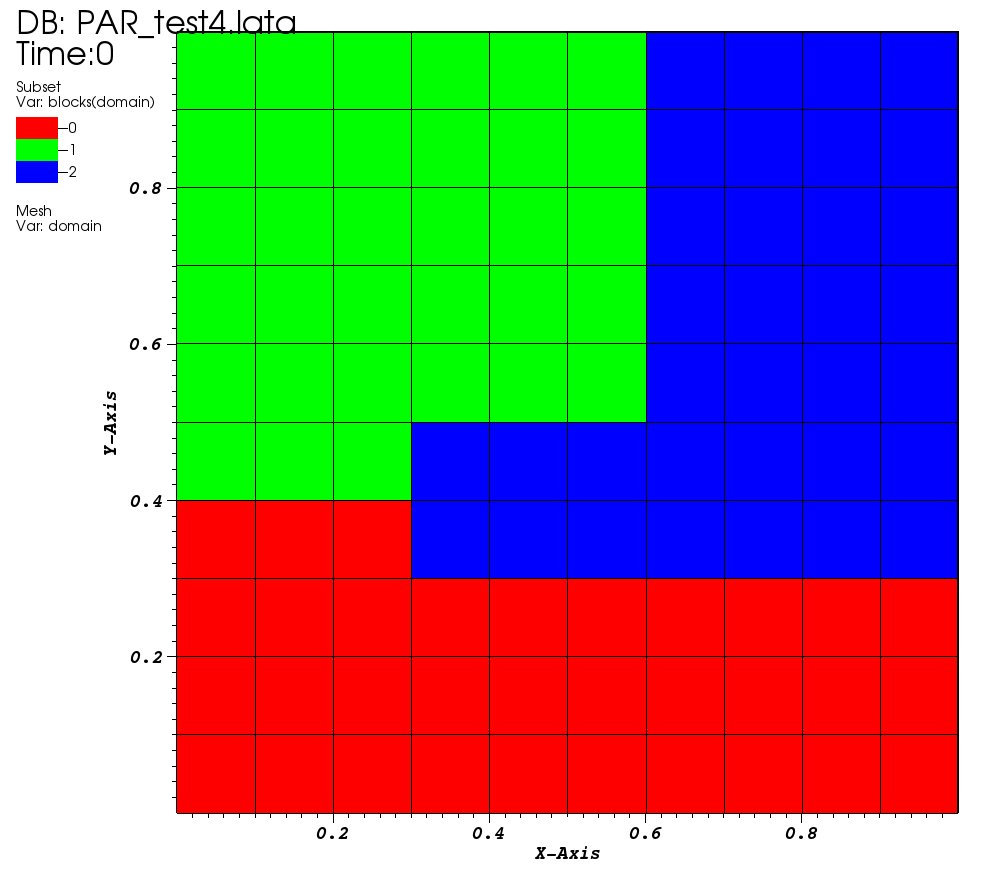
\includegraphics[width=0.45\textwidth]{partition_metis.jpeg} & & 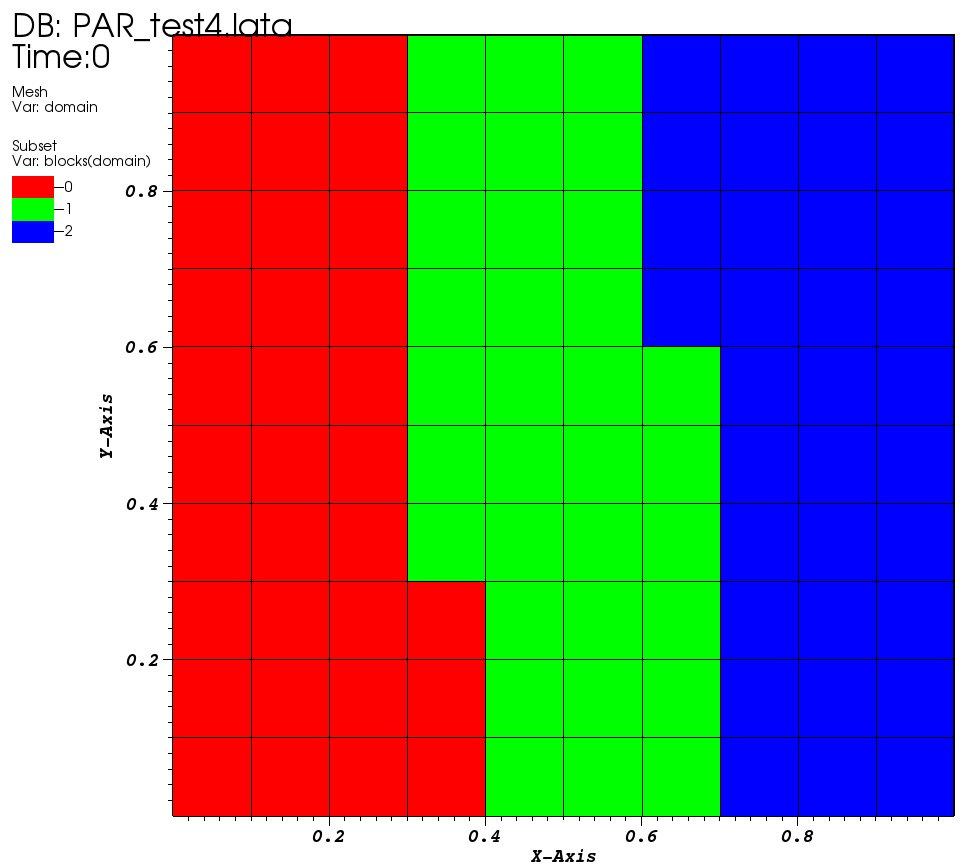
\includegraphics[width=0.45\textwidth]{partition_tranche.jpeg}\tabularnewline
METIS & & Tranche\tabularnewline
\end{tabular}
\par\end{centering}
\caption{Partitioning tools}
\label{partitioning}
\end{figure}

You can see the documentation of \href{\REFERENCEMANUAL\#partition}{this part in the \trustref Reference Manual}.



%%%%%%%%%%%%%%%%%%%%%%%%%%%%%%%%%%%%%%%%%%%%%%%%%
\subsection{Overlapping width value}
%%%%%%%%%%%%%%%%%%%%%%%%%%%%%%%%%%%%%%%%%%%%%%%%%
To make the partitioning, you will have to specify the \underline{overlapping width value}.
This value corresponds to the thickness of the virtual ghost zone (data known by one processor though not owned by it) i.e. the number of vertices or elements on the remote sub-domain known by the local sub-domain (cf Figure \ref{overlap}).

\begin{figure}[h!]
\begin{center}
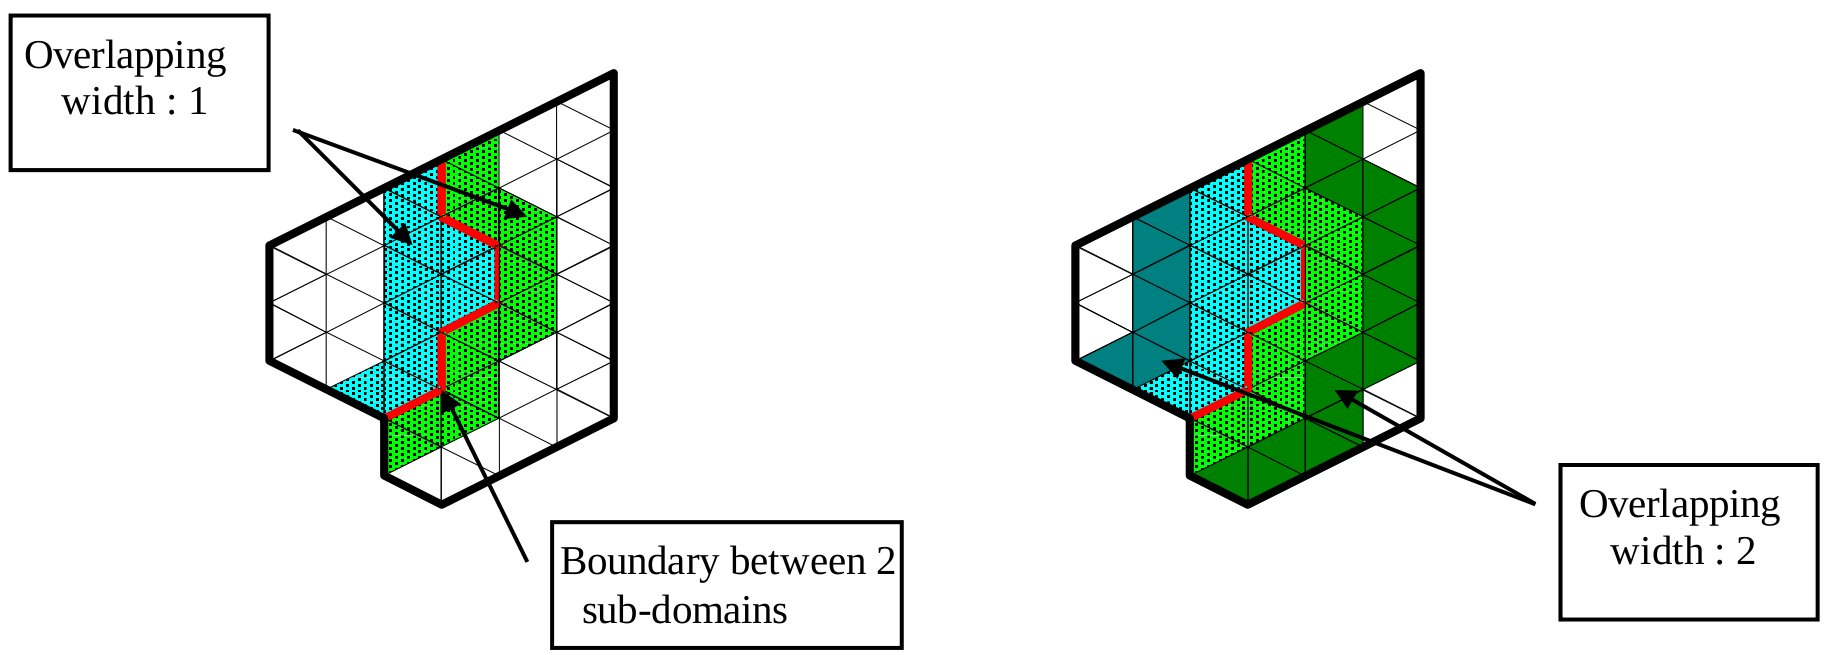
\includegraphics[width=0.96\textwidth]{overlap.jpeg}
\caption{Overlapping width}
\label{overlap}
\end{center}
\end{figure}

This value depends on the space discretization scheme orders:
\begin{itemize}
\item 1 if 1st or 2nd order,
\item 2 if 3rd or 4th order.
\end{itemize}

\Note that in general, you will use "2"!



%%%%%%%%%%%%%%%%%%%%%%%%%%%%%%%%%%%%%%%%%%%%%%%%%%%%%%%%%%%%%%%%%%%%%%%%
\section{Running a parallel calculation}
%%%%%%%%%%%%%%%%%%%%%%%%%%%%%%%%%%%%%%%%%%%%%%%%%%%%%%%%%%%%%%%%%%%%%%%%

%%%%%%%%%%%%%%%%%%%%%%%%%%%%%%%%%%%%%%%%%%%%%%%%%
\subsection{On a PC}
%%%%%%%%%%%%%%%%%%%%%%%%%%%%%%%%%%%%%%%%%%%%%%%%%
To launch the calculation, you have to run the calculation by the usual command completed by the number of processors needed:
\begin{verbatim}
> trust my_parallel_data_file procs_number
\end{verbatim}
and \textit{procs\_number} is the number of processors used. In fact it is the same as the number of sub-domains.\\

You can see the \trust \& \textbf{TrioCFD} user slides in the "Parallel calculation" section for more information and those two exercises of the \trust tutorial: \href{TRUST_tutorial.pdf\#exo_para_1}{exercise 1} and \href{TRUST_tutorial.pdf\#prm_para}{exercise 2}.

%%%%%%%%%%%%%%%%%%%%%%%%%%%%%%%%%%%%%%%%%%%%%%%%%
\subsection{On a cluster}
%%%%%%%%%%%%%%%%%%%%%%%%%%%%%%%%%%%%%%%%%%%%%%%%%
You must submit your job in a queue system.
For this, you must have a submission file.
\trust can create a submission file for you \textbf{on clusters on which the support team has done installations}.
To create this file, run:
\begin{verbatim}
> trust -create_sub_file my_parallel_data_file
\end{verbatim}

You obtain a file named \textbf{"sub\_file"}, you can open it and verify/change values(for example the name of the job, the name of the exe, ...).\\

Then you must submit you calculation with:
\begin{verbatim}
> sbatch sub_file
\end{verbatim}
or 
\begin{verbatim}
> ccc_msub sub_file
\end{verbatim}
following the queue system of the cluster.\\

%You can also run the same command as on a pc:
%\begin{verbatim}
%> trust my_parallel_data_file procs_number
%\end{verbatim}
%\trust will automatically submit your simulation.\\

You can see the \trust \& \textbf{TrioCFD} user slides in the "Parallel calculation" section for more information and \href{TRUST_tutorial.pdf\#exo_para_3}{this exercise of the \trust tutorial}.


%%%%%%%%%%%%%%%%%%%%%%%%%%%%%%%%%%%%%%%%%%%%%%%%%%%%%%%%%%%%%%%%%%%%%%%%
\section{Visualization}
%%%%%%%%%%%%%%%%%%%%%%%%%%%%%%%%%%%%%%%%%%%%%%%%%%%%%%%%%%%%%%%%%%%%%%%%
To visualize your probes, you can use the CurvePlot tool, with the command line:
\begin{verbatim}
> trust -evol my_parallel_data_file
\end{verbatim}
or use Gnuplot or any software which reads values in columns in a file.\\

There are three ways to visualize your parallel results with VisIt:
\begin{itemize}
\item HPCDrive on CCRT/TGCC clusters: opens a deported graphic session on dedicated nodes with more memory (on TGCC cluster: \href{https://visu-tgcc.ccc.cea.fr/HPCDrive/home}{HPCDrive}),
\item local mode: copy your results from the cluster to your local computer and open it with a local parallel version of VisIt with:
\begin{verbatim}
> visit -np 4 &
\end{verbatim}
\end{itemize}

You can have a look at the \trust \& \textbf{TrioCFD} user slides in the "Parallel calculation description" section.




%%%%%%%%%%%%%%%%%%%%%%%%%%%%%%%%%%%%%%%%%%%%%%%%%%%%%%%%%%%%%%%%%%%%%%%%
\section{Useful information}
%%%%%%%%%%%%%%%%%%%%%%%%%%%%%%%%%%%%%%%%%%%%%%%%%%%%%%%%%%%%%%%%%%%%%%%%
%%%%%%%%%%%%%%%%%%%%%%%%%%%%%%%%%%%%%%%%%%%%%%%%%
\subsection{Modify the mesh}
%%%%%%%%%%%%%%%%%%%%%%%%%%%%%%%%%%%%%%%%%%%%%%%%%
If you want to modify your mesh, you have two possibilities:
\begin{itemize} 
\item modify the \textit{my\_data\_file.data} file and run:
\begin{verbatim}
> trust -partition my_data_file [parts_number]
\end{verbatim}
Be carefull it will erase the \textit{SEQ\_my\_data\_file.data}, \textit{DEC\_my\_data\_file.data} and \\
\textit{PAR\_my\_data\_file.data} files and creates new ones.\\
Then it will run the new \textit{DEC\_my\_data\_file.data} file which gives your new \textit{DOM\_000n}\textbf{.Zones} files.

\item modify the meshing part of file \textit{DEC\_my\_data\_file.data} and run it with:
\begin{verbatim}
> trust DEC_my_data_file
\end{verbatim}
\end{itemize}

Then run the parallel calculation normally, on the new \textit{DOM\_000n}\textbf{.Zones} files.
\begin{verbatim}
> trust PAR_my_data_file procs_number
\end{verbatim}




%%%%%%%%%%%%%%%%%%%%%%%%%%%%%%%%%%%%%%%%%%%%%%%%%
\subsection{Modify calculation parameters}
%%%%%%%%%%%%%%%%%%%%%%%%%%%%%%%%%%%%%%%%%%%%%%%%%
If you want to modify the calculation parameters, you can modify:
\begin{itemize} 
\item the file \textit{my\_data\_file.data} and run:
\begin{verbatim}
> trust -partition data_file_name [parts_number]
\end{verbatim}
But it will erase the \textit{SEQ\_my\_data\_file.data}, \textit{DEC\_my\_data\_file.data} and \\
\textit{PAR\_my\_data\_file.data} files and create new ones.\\
Then it will run the new \textit{DEC\_my\_data\_file.data} file which gives your new \textit{DOM\_000n}\textbf{.Zones} files.\\
\Note that in that case, you don't need to re-create the mesh so you can use the second point below:
\item modify the \textit{PAR\_my\_data\_file.data} file \underline{without} running "trust -partition datafile" command line.
\end{itemize}
Then run the \textit{PAR\_my\_data\_file.data} file with:
\begin{verbatim}
> trust PAR_my_data_file procs_number
\end{verbatim}

\Note that if after a certain time, you want to reopen an old case and understand want you did in it without any doubts, you may create two files by hands:
\begin{itemize} 
\item one "BuildMeshes.data" file only for the mesh and the cut of the mesh, and
\item one "calculation.data" file for the parallel calculation. 
\end{itemize}
You will run it like:
\begin{verbatim}
> trust BuildMeshes
> trust calculation processors_number
\end{verbatim}

For this point, you can have a look at \href{TRUST_tutorial.pdf\#prm_para}{this exercise of the \trust tutorial}.






%%%%%%%%%%%%%%%%%%%%%%%%%%%%%%%%%%%%%%%%%%%%%%%%%%%%%%%%%%%%%%%%%%%%%%%%



%%%%%%%%%%%%%%%%%%%%%%%%%%%%%%%%%%%%%%%%%%%%%%%%%%%%%%%%%%%%%%%%%%%%%%%%%%
%%%
%%\chapter{Automatic validation form}
%%%
%%%%%%%%%%%%%%%%%%%%%%%%%%%%%%%%%%%%%%%%%%%%%%%%%%%%%%%%%%%%%%%%%%%%%%%%%%
%%%\input{chap8_prm.tex}
%%%%%%%%%%%%%%%%%%%%%%%%%%%%%%%%%%%%%%%%%%%%%%%%%%%%%%%%%%%%%%%%%%%%%%%%%%



\end{document}

